\documentclass[11pt, a4paper, titlepage]{report}
\title{ZIWM - Sprawozdanie}
\usepackage{comment}
\usepackage[utf8]{inputenc} 
\usepackage[T1]{fontenc}
\linespread{1.2}
\usepackage[polish]{babel}
\usepackage{polski}
\usepackage{graphicx} 
\usepackage{enumitem}
\usepackage{float}
\usepackage[hidelinks]{hyperref}
\usepackage{afterpage}
\usepackage{listings}
\usepackage{color}
\usepackage{courier}
\usepackage{listings}
\usepackage[most]{tcolorbox}
\usepackage{mdframed}

\addtolength{\textwidth}{3.5cm}
\addtolength{\hoffset}{-2cm}
\addtolength{\textheight}{3.5cm}
\addtolength{\voffset}{-2cm}
\usepackage{indentfirst}
\usepackage{caption}
\usepackage{graphicx}
\usepackage[rightcaption]{sidecap}
\graphicspath{ {images/} }
\definecolor{mygreen}{rgb}{0,0.6,0}
\definecolor{mygray}{rgb}{0.5,0.5,0.5}
\definecolor{mymauve}{rgb}{0.58,0,0.82} 
\definecolor{codegreen}{rgb}{0,0.6,0}
\definecolor{gray}{rgb}{0.5,0.5,0.5}
\definecolor{numcolour}{rgb}{0.75,0.75,0.75}
\definecolor{codepurple}{rgb}{0.58,0,0.82}
\definecolor{backcolour}{rgb}{0.97,0.97,0.97}

\renewcommand\lstlistlistingname{Spis listingów}
\lstset{ %
	backgroundcolor=\color{backcolour}, 
	rulecolor=\color{gray},  
    commentstyle=\color{gray},
    keywordstyle=\color{magenta},
    basicstyle=\footnotesize\ttfamily\small,
    numberstyle=\footnotesize\ttfamily\small\color{numcolour},
    stringstyle=\color{codepurple},
    breakatwhitespace=false,         
    breaklines=true,                 
    captionpos=b,                    
    keepspaces=true,                 
    numbers=left,                    
    numbersep=10pt,                  
    showspaces=false,                
    showstringspaces=false,
    showtabs=false,                  
    tabsize=1,
    framexleftmargin=22pt,
    framexbottommargin=5pt,
    framextopmargin=5pt,
    frame=single
}

\date{Wrocław, 1.06.2016}
\makeatletter
\renewcommand{\maketitle}{\begin{titlepage}
		\begin{center}\small
			Politechnika Wrocławska\\
			Wydział Elektroniki\\
			Rok akad. 2015/2016\\
			Kierunek Informatyka\\
			\vspace{3cm}
			\rule{\linewidth}{0.4pt}
				\huge \textsc{\textbf{Zastosowania Informatyki w Medycynie}}
				\vspace{0.5cm} \\
				\normalsize \textit{Projekt - "Badanie różnych typów komitetów klasyfikatorów"}  
			\rule{\linewidth}{0.4pt}           
		\end{center}
		
		\vspace{3cm}
		\begin{flushleft}
			\textbf{\textit{Grupa projektowa:}} \hspace{8.0cm} \textbf{\textit{Prowadzący:}} \\
			Grzegorz Zając, 200664 \hfill{dr inż. Bartosz Krawczyk} \\	
            Sebastian Bujwid, 200736\\
            Jakub Wężykowski, 200813\\
			\vspace{0.5cm}
			\textbf{\textit{Termin:}}\\ Czwartek 11:15\\
			\vspace{2cm}		
		\end{flushleft}
		\vspace*{\stretch{6}}
		\begin{center}
			\@date
		\end{center}
	\end{titlepage}%
}
\makeatother
\begin{document}
\maketitle
\tableofcontents
\cleardoublepage
\phantomsection
\addcontentsline{toc}{chapter}{\listfigurename}


\chapter{Wstęp}
\section{Cel projektu}
Celem projektu było przetestowanie następujących algorytmów:

\begin{itemize}
\item pojedyncza sieć neuronowa ze wsteczną propagacją błędu (BPNN - \textit{Back Propagation Neural Network})
\item pojedyncza sieć neuronowa typu Extreme Learning Machine (ELM) \cite{ELM}
\item komitet ELM wykorzystujący losowe generowanie sieci i głosowanie większościowe \cite{ELM_Random}
\item komitet ELM bazujący na \textit{Bagging} (różne obiekty uczące)
\item komitet ELM bazujący na \textit{Random Subspace} (różne cechy)
\end{itemize}

Zbadanie działania algorytmów należało przeprowadzić na co najmniej 15 różnorodnych bazach danych z \textit{UCI ML Repository}\cite{UCI_ML_Repo}.

Dodatkowo, w ramach projektu trzy typy komitetów klasyfikatorów (\textit{Bagging}, \textit{Random Subspace}, Randomizacja) zostały zbadane z użyciem dwóch dodatkowych klasyfikatorów (Śeć neuronowa z propagacją wsteczną oraz Support Vector Machine). 

Co więcej, wszystkie kombinacje typów komitetów oraz ich członków zostały zasymulowane przy użyciu dwóch różnych wersji modułu decyzyjnego komitetu - kombinacja wyników częściowych poszczególnych członków komitetów została przeprowadzona za pomocą głosowania większościowego i przy użyciu średniej arytmetycznej (wyliczanej ze wsparć dla każdej z klas).

\section{Zakres projektu}
\textbf{W zakres projektu wchodziło: }
\begin{enumerate}


\item Zaprojektowanie systemu pozwalającego na przeprowadzenie kompleksowych badań.
\item Wykorzystanie gotowych implementacji dwóch typów klasyfikatorów bazowych:
\begin{itemize}
\item sieć neuronowa ze wsteczną propagacją błędów
\item Extreme Learning Machine
\end{itemize}
\item Implementacja trzech typów komitetów:
\begin{itemize}
\item \textit{Random Networks}
\item \textit{Bagging}
\item \textit{Random Subspace}
\end{itemize}
\item Przeprowadzenie badań wyznaczających skuteczność zaimplementowanych rozwiązań
\item Zbadanie wpływu liczby członków komitetu na jego działanie
\item Interpretacja wyników i wywnioskowanie zależności pomiędzy skutecznością, a badanym zestawem klasyfikującym
\item Porównanie czasów uczenia Sieci Neuronowej z Wsteczną Propagacją oraz Extreme Learning Machine
\end{enumerate}

\textbf{Zakres podstawowy został rozszerzony o:}
\begin{enumerate}
\item Implementacja dwóch typów modułu decyzyjnego wewnątrz każdego komitetu:
\begin{itemize}
\item głosowanie większościowe
\item głosowanie wykorzystujące średnią arytmetyczną
\end{itemize}
\item Zbadanie wpływu metody kombinowania rozwiązań częściowych w komitecie
\item Zbudowanie komitetów homogenicznych składających się Sieci Neuronowych z Wsteczną Propagacją oraz Support Vector Machine
\item Zbadanie wpływu typu członków na działanie komitetu
\item Wykorzystanie dwóch różnych implementacji sieci neuronowych ze wsteczną propagacją (PyBrain, NeuroLab) oraz dwóch różnych implementacji ELM (HPELM, Python Extreme Learning Machine) w celu wyboru odpowiedniejszych.
\end{enumerate}


\chapter{Opis zaimplementowanego systemu}
\section{Architektura systemu}
System został zaprojektowany oraz zaimplementowany w taki sposób, aby mógł być w łatwy sposób rozszerzalny. Dzięki zastosowaniu obiektowego paradygmatu programowania system ma strukturę niezależnych modułów. Możliwe jest zastosowanie dowolnego typu klasyfikatora niezależnie od użytego typu komitetu. Dodatkowo, tak samo można użyć dowolny moduł decyzyjny w każdym typie komitetu. Konieczne jest jedynie implementowanie określonego interfejsu klasyfikatora, komitetu oraz modułu decyzyjnego - odbywa się to poprzez dziedziczenie po utworzonych klasach. Powstało także wiele narzędzi, dzięki którym zaimplementowany system stanowi środowisko 

Infrastruktura systemu pozwala na:
\begin{itemize}
\item wczytywanie wszystkich zestawów danych z zadanych katalogów
\item odpowiednie przetwarzanie zestawów w automatyczny sposób - skalowanie, normalizacja lub kodowanie w systemie OHE atrybutów
\item zautomatyzowane rysowanie wykresów za pomocą zaimplementowanych skryptów
\item wyznaczenie skuteczności modeli
\item uruchomienie automatycznych testów uwzględniających wszystkie dostępne zbiory danych, modele, komitety i systemy głosowania.
\end{itemize}

Zaimplementowany system stanowi wygodne środowisko do badania skuteczności komitetów w zależności od typu i liczby członków, modułu decyzyjnego oraz zbioru danych ze względu na fakt, że wszystkie te elementy mogą być łatwo wymieniane oraz rozszerzane.

\section{Klasyfikatory}
\subsection{Sieć neuronowa ze wsteczną propagacją}
Podstawowym klasyfikatorem bazowym użytym w projekcie była sieć neuronowa uczona przy użyciu wstecznej propagacji błędu. Wykorzystano implementację tego typu sieci z biblioteki PyBrain. Biblioteka ta posiada także algorytm trenujący wykorzystujący wsteczną propagację.

Użyta biblioteka pozwala na zbudowanie sieci neuronowej z gotowych modułów, jednak istnieją również metody pozwalające skrócić proces konfiguracji sieci. Najpierw określa się liczbę i rozmiar warstw sieci. W opisywanym rozwiązaniu użyto trzech warstw: wejściowa o rozmiarze równym liczbie cech, wyjściowa o rozmiarze równym liczbie klas oraz ukryta warstwa o rozmiarze równym średniej arytmetycznej rozmiarów pozostałych warstw. Jako funkcja aktywacji wykorzystano Sigmoid. W warstwie wejściowej oraz ukrytej dodane zostało obciążenie w postaci neuronów o stałej wadze równej 1 (ang. \textit{bias}).
Po utworzeniu sieci następuje jej trenowanie przy użyciu propagacji wstecznej błędu.

\subsection{Extreme Learning Machine}
ELM jako klasyfikator bazowy był oparty na gotowej implementacji z biblioteki \textit{HPELM - High-Performance implementation of an Extreme Learning Machine} \ref{HPELM}. Nie wymagała ona od nas ręcznej konstrukcji sieci, ani implementacji procesu uczenia. Twórcy biblioteki mówią o niej, że ma ona wysoką wydajność.

\subsection{Support Vector Machine}
Jako punkt odniesienia do klasyfikatorów opartych na sieciach neuronowych, został użyty również SVM. On również opierał się na gotowej implementacji z biblioteki \textit{scikit-learn} \ref{scikit-learn}. Problem klasyfikacji wieloklasowej został zrealizowany poprzez rozwiązanie wielu problemów klasyfikacji binarnej oraz agregacje wyników zgodnie z ideą \textit{One vs all}.

\section{Komitety}
\subsection{Random Networks}
Pierwszym typem komitetu klasyfikatorów utworzonym na potrzeby projektu jest komitet składający się z losowych sieci. Klasyfikatory w tym komitecie uczą się na tych samych danych, jednak różnią się początkowym stanem (losowe wagi początkowe w neuronach sieci). Pozwala to wyeliminować efekt osiągnięcia przez pojedynczy klasyfikator minimum lokalnego. 
\subsection{Bagging}
Kolejny typ komitetu bazuje na idei uczenia pojedynczych klasyfikatorów na różnych danych. Najpierw dla każdego klasyfikatora losowana jest próbka danych ze zwracaniem (ang. \textit{bootstrap sample}) i dany klasyfikator uczony jest na tej próbce. Następnie podczas rozpoznawania wyniki poszczególnych klasyfikatorów są agregowane, stąd nazwa \textit{bagging} (ang. \textit{bootstrap aggregating}).
\subsection{Random Subspace}
Ostatnim zaimplementowanym typem komitetu jest komitet klasyfikatorów uczonym na różnych podprzestrzeniach cech. Metoda podobnie jak \textit{Bagging} dzieli zbiór danych na różne podzbiory, jednak w przypadku \textit{Random Subspace} klasyfikatory uczą się tu na wybranych losowo podzbiorach cech, wykorzystując do tego wszystkie obiekty należące do zestawu uczącego.

Podczas treningu klasyfikatorów, dla każdego z nich generowany jest oddzielny zestaw uczący zawierający losowo wybrane 50\% wszystkich cech. Przy implementacji metody uczącej należało zwrócić uwagę na dwie kwestie. Po pierwsze, należy zapisać indeksy cech wykorzystanych do nauki każdego z klasyfikatorów, ponieważ są one potrzebne przy rozpoznawaniu obiektów ze zbioru testującego. Po drugie, niektóre cechy, określające kategorię a nie wartość rzeczywistą, zostały przekonwertowane do kodu 1 z n, przez co zostały zapisane na kilku kolumnach macierzy uczącej. Wymusiło to wprowadzenie metadanych określających, które kolumny macierzy odpowiadają której cesze, a następnie podczas losowania podzbioru wybranie wszystkich kolumn danej cechy. Dzięki temu klasyfikatory otrzymywały pełną informację o danej cesze określającej kategorię.


\section{Systemy głosowania}
\subsection{Głosowanie większościowe}
Jednym z wykorzystanych typów głosowania wewnątrz komitetu jest głosowanie większościowe. Najpierw dla każdego klasyfikatora bazowego określana jest klasa o najwyższym wsparciu w danym klasyfikatorze. Następnie sumowane są wyniki dla każdej z klas i klasa z największą liczbą wspierających klasyfikatorów jest wybierana.
\subsection{Ciągłe odpowiedzi}
Ze względu na to, że agregacja wyników cząstkowych poprzez \textit{głosowanie większościowe} w żaden sposób nie uwzględnia pewności podejmowanych decyzji, zaimplementowany został inny sposób agregacji wyników poprzez łączenie ciągłych odpowiedzi w postaci wektorów wsparć od poszczególnych klasyfikatorów.

\section{Zestawy danych}
\subsection{Wykorzystane zestawy danych}

Do przeprowadzenia badań wykorzystane zostało 15 różnorodnych baz danych z UCI ML Repository \cite{UCI_ML_Repo}.	

Zestawy danych zostały dobrane w taki sposób, aby przeprowadzić pomiary skuteczności działania zastosowanych modeli w zróżnicowanych środowiskach.

Wybrane zostały zestawy zarówno o dużej jak i małej liczbie obiektów uczących - od kilkudziesięciu do kilkuset. Podobnie w przypadku liczby cech - dobrane zostały zestawy od kilku cech do prawie stu pięćdziesięciu. Została także zwrócona uwaga na typ cech - uwzględniono zestawy o wyłącznie danych o wartościach rzeczywistych, wyłącznie danych o wartościach dyskretnych oraz zestawy mieszane. Bazy danych, które zostały wykorzystane, dotyczą różnych dziedzin techniki oraz nauki.

Ponadto zadbano o wyszukanie zbiorów danych o stosunkowo równomiernym rozkładzie klas, co okazało się istotne z powodu wykorzystania do walidacji metody k-fold.

Zbiory danych zostały poddane dodatkowemu przetworzeniu przed wykorzystaniem do badań. Cechy o charakterze przynależności do kategorii były poddawane systemowi kodowania OHE. Natomiast cechy o charakterze ciągłym były poddane skalowaniu do zakresu od $0.0$ do $1.0$.

Podstawowe informacje o użytych zestawach danych zostały przedstawione w tabeli \ref{tbl:datasets}.

\begin{center}
\begin{table}
\caption{Wykorzystane zestawy danych}
\centering
\begin{tabular}{c || c | c}
Nazwa zbioru & liczba cech & liczba obiektów \\ \hline
\textit{breast\_cancer} 		& 89 	& 286 \\
\textit{crx} 					& 15	& 653 \\
\textit{dermatology}			& 34	& 358 \\
\textit{house\_votes}			& 16	& 435 \\
\textit{inosphere}				& 34	& 352 \\
\textit{iris}					& 4		& 150 \\
\textit{soybean\_small}			& 35	& 47  \\
\textit{spect}					& 22	& 267 \\
\textit{thyroid}				& 5		& 215 \\
\textit{tic\_tac\_toe}			& 9		& 958 \\
\textit{urban\_land\_cover}		& 147	& 675 \\
\textit{wine}					& 13	& 178 \\
\textit{yeast}					& 8		& 1147
\label{tbl:datasets}
\end{tabular}
\end{table}
\end{center}

\iffalse
\begin{enumerate}
\item Breast Cancer
\item Iris
\item Dermatology
\item Wine
\item Soybean Small
\item Glass
\item Ionosphere
\item Congresional Votes
\item Thyroid
\item Heart SPECT (Single Proton Emission Computed Tomography)
\item Credit Approval
\item Tic-Tac-Toe end game
\item Urban land cover
\item Yeast
\item Soybean large
\end{enumerate}
\fi

\subsection{Problem wartości brakujących}
W niektórych zestawach danych wykorzystanych do przeprowadzenia badań pojawiał się problem wartości brakujących (np. w zbiorach dotyczących danych medycznych wynikający z niemożności przeprowadzenia wszystkich badań u szczególnych pacjentów). Niestety, ciężko nam było przewidzieć zachowanie wykorzystywanych metod klasyfikacji w przypadku niepełnego zbioru danych. 

W przypadku, gdy liczba brakujących danych jest stosunkowo niewielka możliwe jest zastosowanie najprostszej metody polegającej na usunięciu niewielkich grup obiektów posiadających niepełny zestaw wartości atrybutów. 

Jednakże w innych sytuacjach nie warto usuwać obiektów lub atrybutów z takimi wartościami, lecz zastosować metody ich uzupełniania. Jedną z metod jest uzupełnianie niewiadomych średnimi pojedynczej cechy. Kolejna metoda zakłada wykorzystanie mediany pojedynczej cechy. W przypadku dużej liczby brakujących danych oraz założeniu całkowitej losowości braków danych (MCAR ang. missing completely at random) warto wykonywać uzupełnienia specjalnymi metodami takimi jak: metody regresyjne, metoda estymacji i maksymalizacji oraz wielokrotna imputacja.

Ostatecznie założyliśmy, że brakujące wartości nie były związane ze strukturą informacji o różnicowaniu grup i usunęliśmy niewielkie grupy obiektów dotknięte zjawiskiem brakujących wartości atrybutów.
Zgodnie z uzyskanymi informacjami, w przypadku dużych zbiorów danych i stosunkowo niewielkich strat taka procedura nie stwarza problemu.

\section{Metodologia wykonywania badań}

W przeprowadzonych badaniach komitetów mierzoną metryką było skuteczność klasyfikacji (ang. \textit{accuracy}), czyli iloraz liczby poprawnie rozpoznanych obiektów przez całkowitą ich liczbę.
Przedstawione wartości są średnimi wynikami z 10-krotnej warstwowej walidacji krzyżowej z zachowaniem rozkładu klasy (ang. \textit{stratified 10-fold cross validation}). Zbiory danych zostały indywidualnie podzielone na 10 podzbiorów (ang. \textit{fold}). Następnie wykonano iteracje w których modele były uczone na każdej parze 9 podzbiorów, a testowane na 1 pozostałym.

Wykonane zostały również badania skuteczności pojedynczych klasyfikatorów oraz ich czasu uczenia liczonego dla poszczególnych zbiorów danych jako suma 10 czasów uczenia z poszczególnych iteracji walidacji krzyżowej.

\chapter{Analiza wyników przeprowadzonych badań}

\section{Klasyfikatory bazowe}
\subsection{Skuteczność}
Wartość skuteczności pojedynczego klasyfikatora bazowego waha się w przedziale od 55\% do 98\% w zależności od rozpatrywanego zbioru danych. Parametry sieci neuronowych zostały dobrane w taki sposób, aby osiągnąć wysoką skuteczność w jak największej liczbie zbiorów danych z zachowaniem rozsądnego czasu uczenia sieci. Z tego powodu w niektórych zbiorach skuteczność pojedynczego klasyfikatora jest niska. Pozwala to jednak dostrzec przewagę niektórych typów komitetu nad pojedynczą siecią neuronową.
\subsection{Czasy uczenia}
Jednym z aspektów projektu było porównanie sieci ELM ze zwykłymi sieciami neuronowymi. W szczególności należało zwrócić uwagę na czas nauki każdego klasyfikatora. Przeprowadzenie badań dla klasyfikatora ELM zajęło około 2 godzin na jednym komputerze posiadającym 4-rdzeniowy procesor. W przypadku zwykłych sieci neuronowych do przeprowadzenia badań użyto dwóch 36-rdzeniowych maszyn, aby jak najlepiej zrównoleglić obliczenia. Mimo maszyn o tak dużej mocy obliczeniowej, przeprowadzenie pełnych badań dla sieci neuronowych zajęło około 20 godzin. Wynika z tego, iż klasyfikatory ELM potrzebowały o dwa rzędy wielkości mniej czasu niż zwykłe sieci neuronowe, osiągając tym samym bardzo zbliżoną skuteczność.

\begin{figure}[H]
	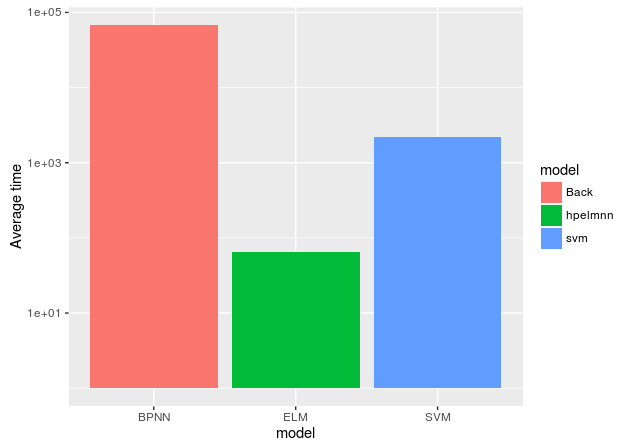
\includegraphics[width=0.6\textwidth]{base_classifier_time}
    \centering
    \caption{Czasy uczenia pojedynczych klasyfikatorów - skala logarytmiczna}
    \label{fig:base_classifiers_time}
\end{figure}

\begin{figure}[H]
	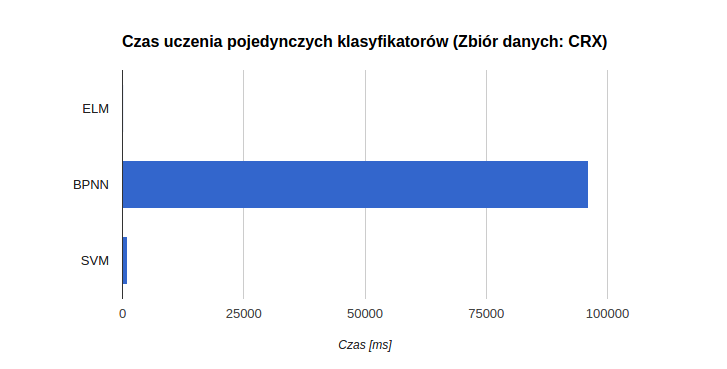
\includegraphics[width=1.0\textwidth]{wykres-czas}
    \centering
    \caption{Porównanie czasów uczenia pojedynczych klasyfikatorów - skala liniowa}
    \label{fig:time}
\end{figure}

\section{Wyniki komitetów}

W ramach badań sprawdzona została skuteczność działania komitetów typu: 
\begin{itemize}
\item \textit{Bagging}
\item \textit{Random Subspace}
\item \textit{Random Networks} 
\end{itemize}
składających się z 3 typów modeli: 
\begin{itemize}
\item Sieć neuronowa z propagacją wsteczną
\item Extreme Learning Machine
\item Support Vector Machine
\end{itemize}
dla dwóch typów modułów decyzyjnych:
\begin{itemize}
\item głosowanie większościowe
\item średnia arytmetyczna wsparć dla poszczególnych klas.
\end{itemize}

Wyniki wszystkich przeprowadzonych symulacji zostały przedstawione na zbiorczym wykresie \ref{fig:overall}.

\begin{figure}[h]
	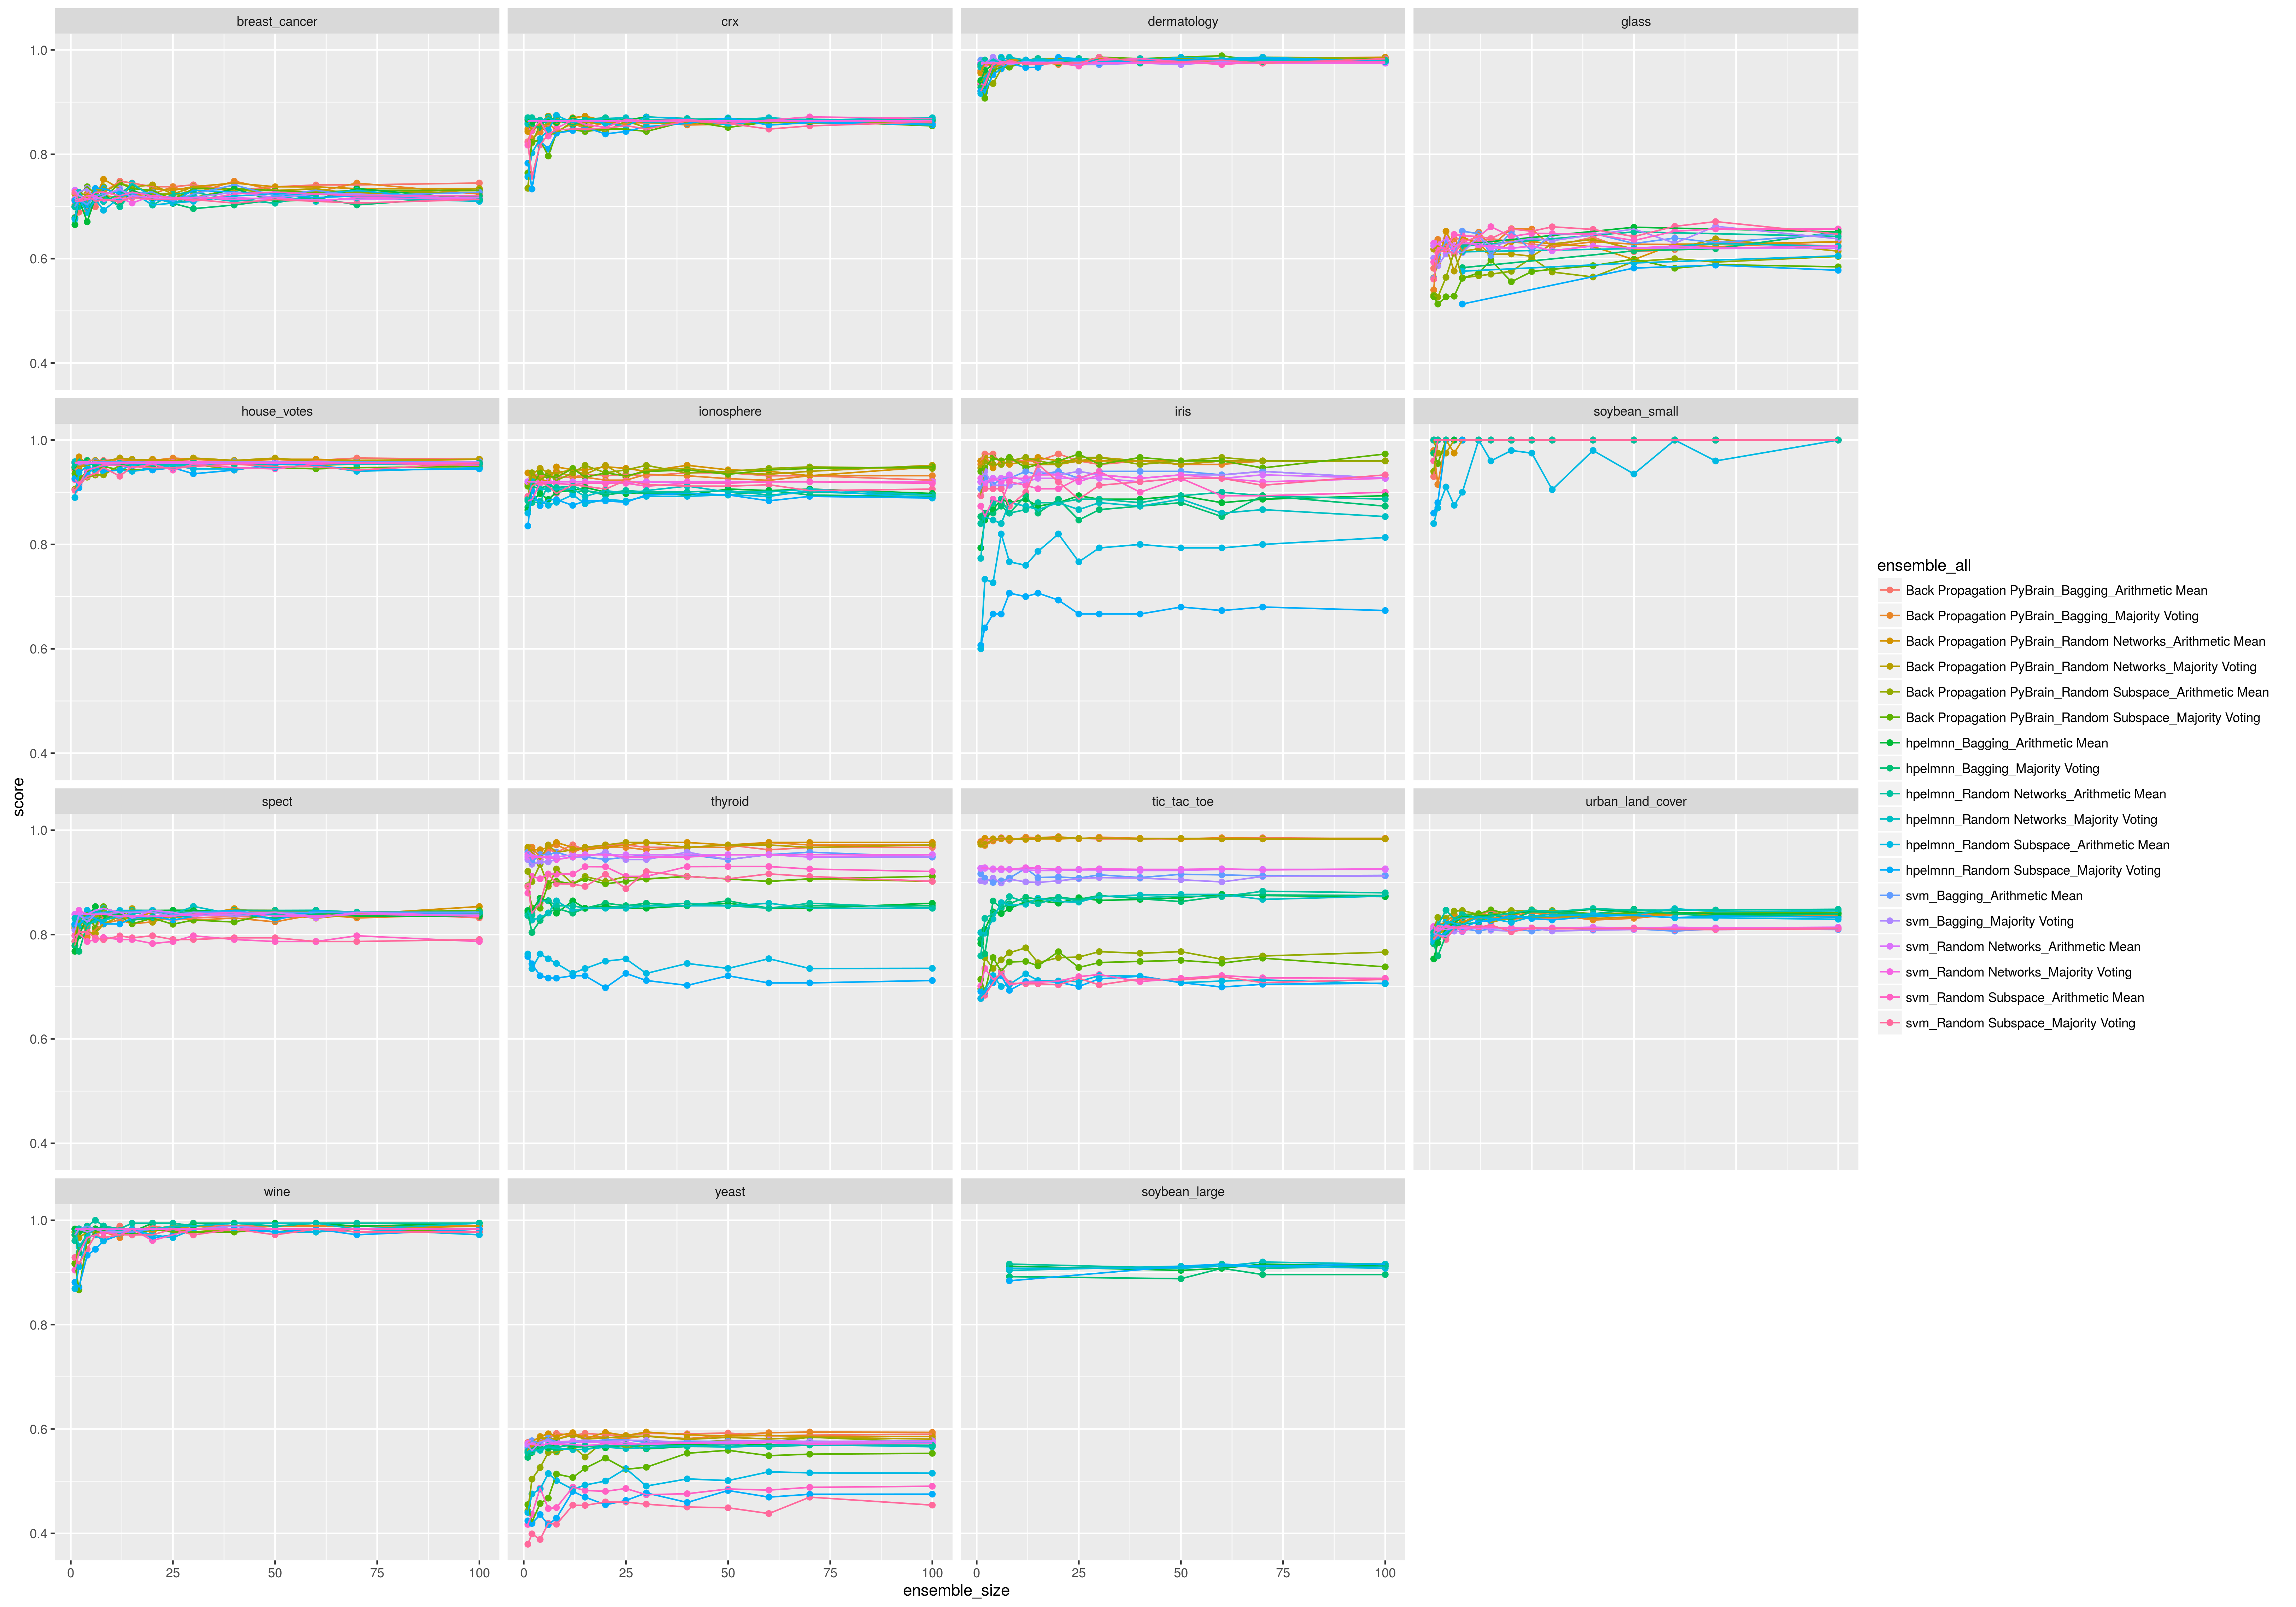
\includegraphics[height=1.0\textwidth,keepaspectratio, angle=90]{overall}
    \centering
    \caption{Zbiorowe wyniki wszystkich przeprowadzonych symulacji na wszystkich zbiorach danych}
    \label{fig:overall}
\end{figure}

Na rysunku \ref{fig:type2_breast} przedstawione zostały przykładowe wyniki badań - w tym wypadku dla zbioru \textit{breast\_cancer}, natomiast na rysunku \ref{fig:type2_spect} ze zbioru \textit{spect}.

\begin{figure}[H]
	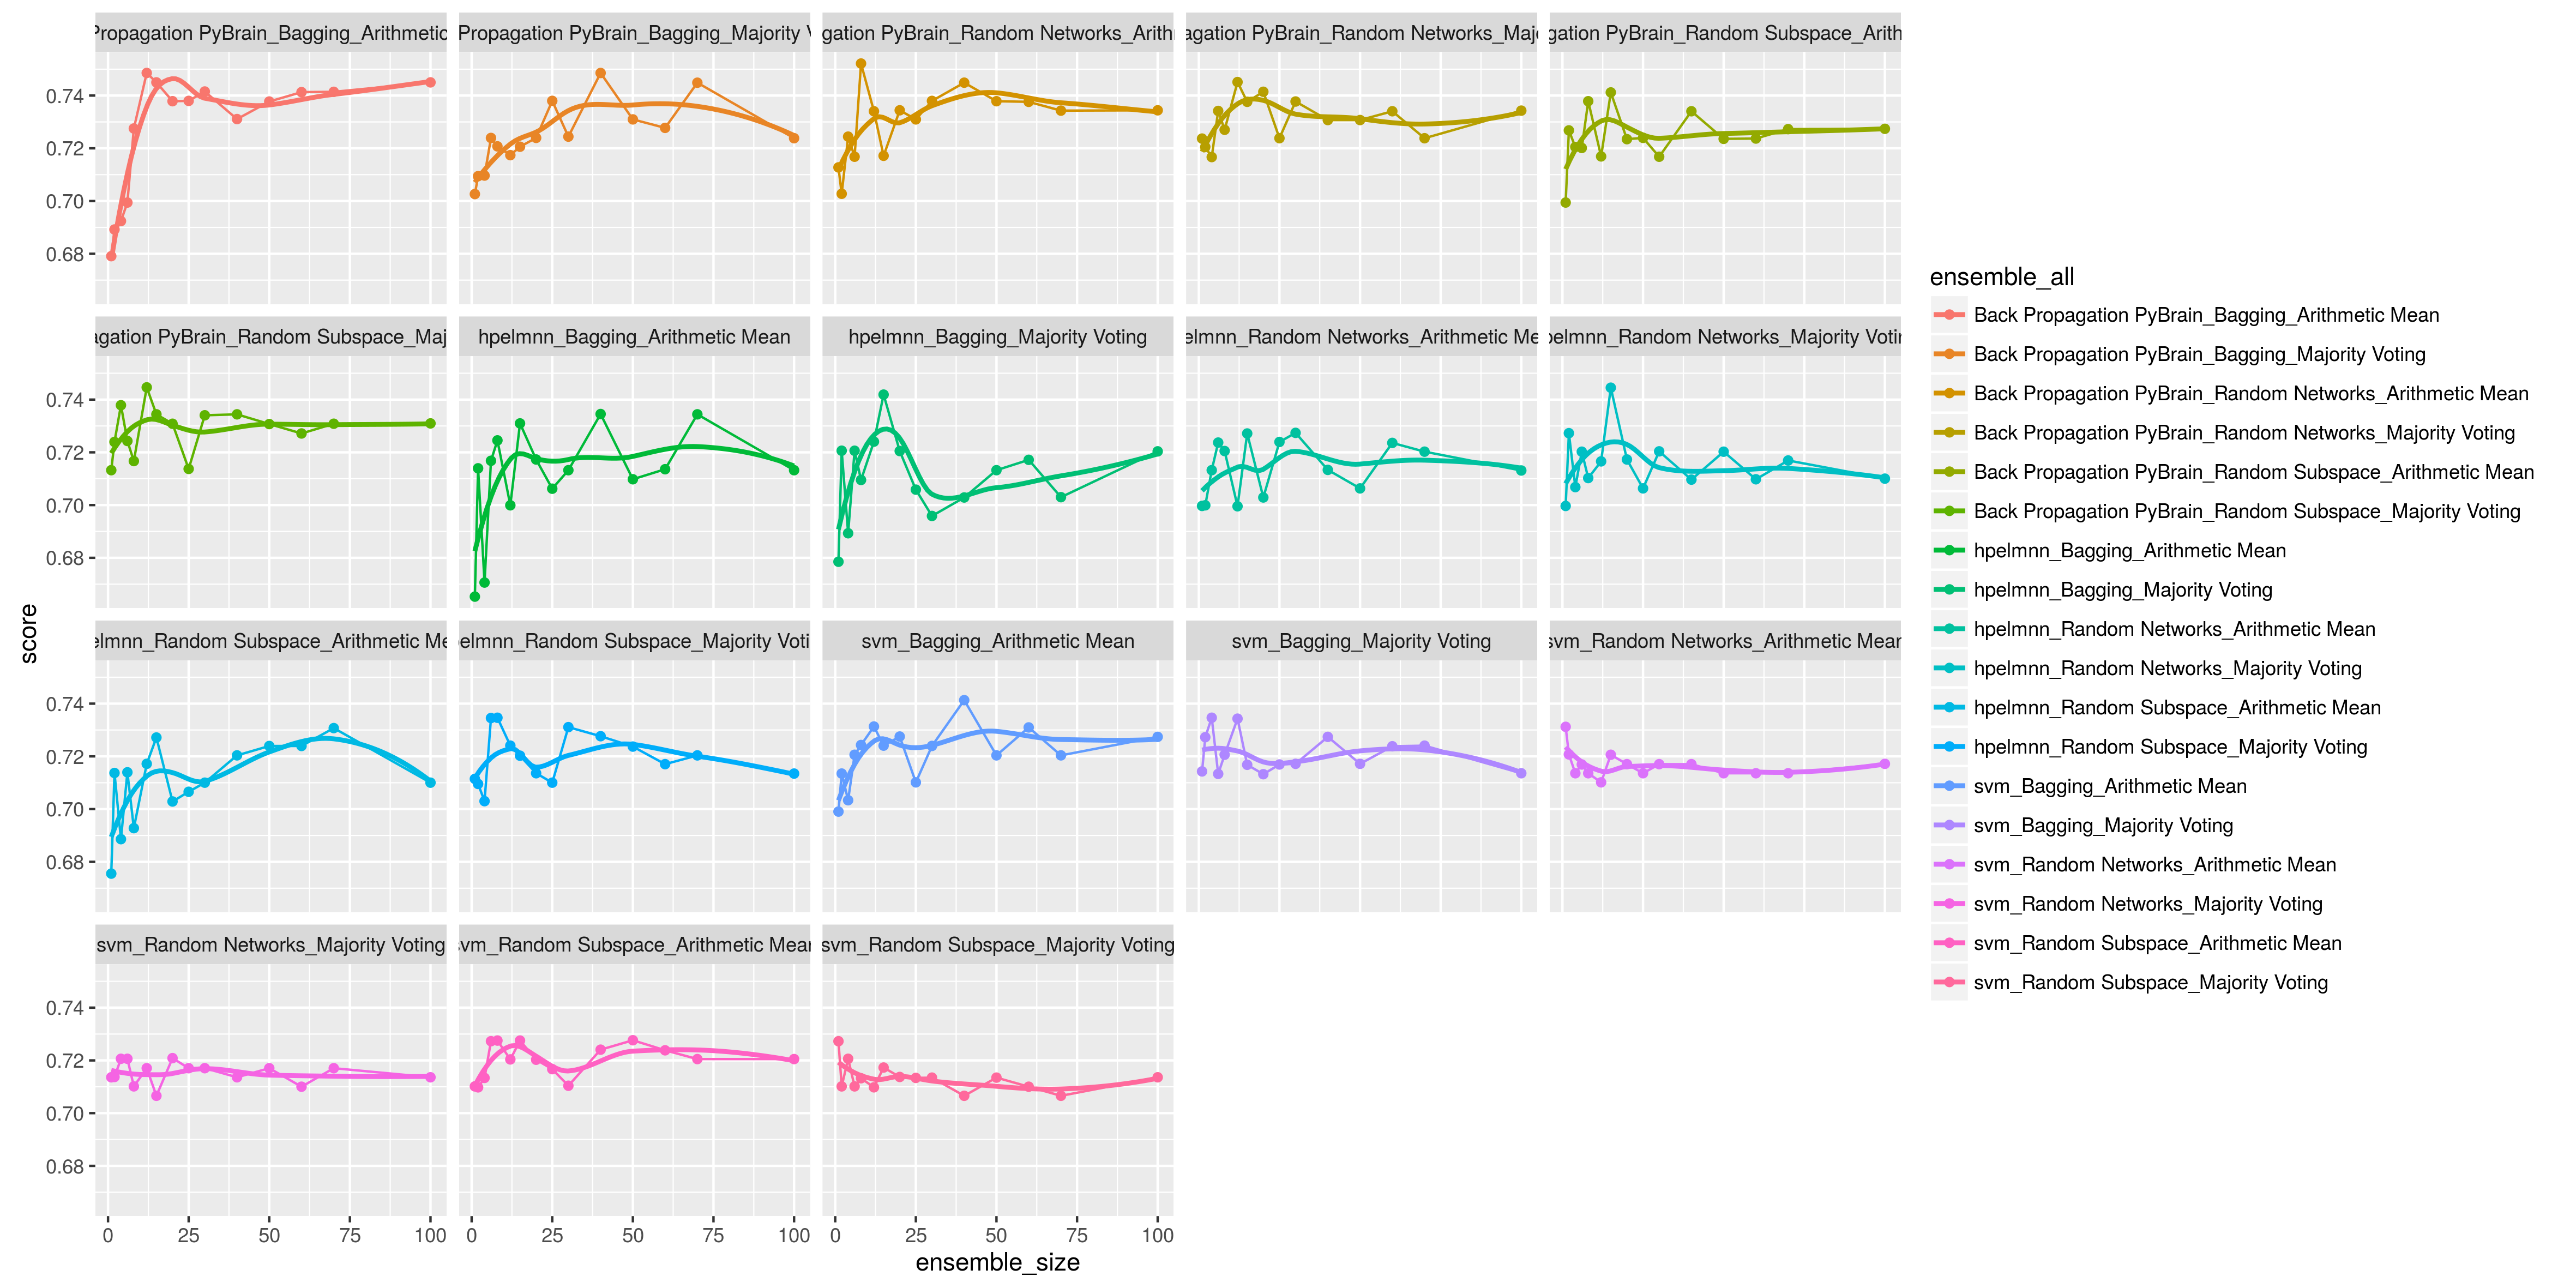
\includegraphics[width=1.0\textwidth]{type2_score_size_model_breast_cancer}
    \centering
    \caption{Skuteczność komitetów, \textit{breast\_cancer} - 89 cech, 286 obiektów}
    \label{fig:type2_breast}
\end{figure}

\begin{figure}[H]
	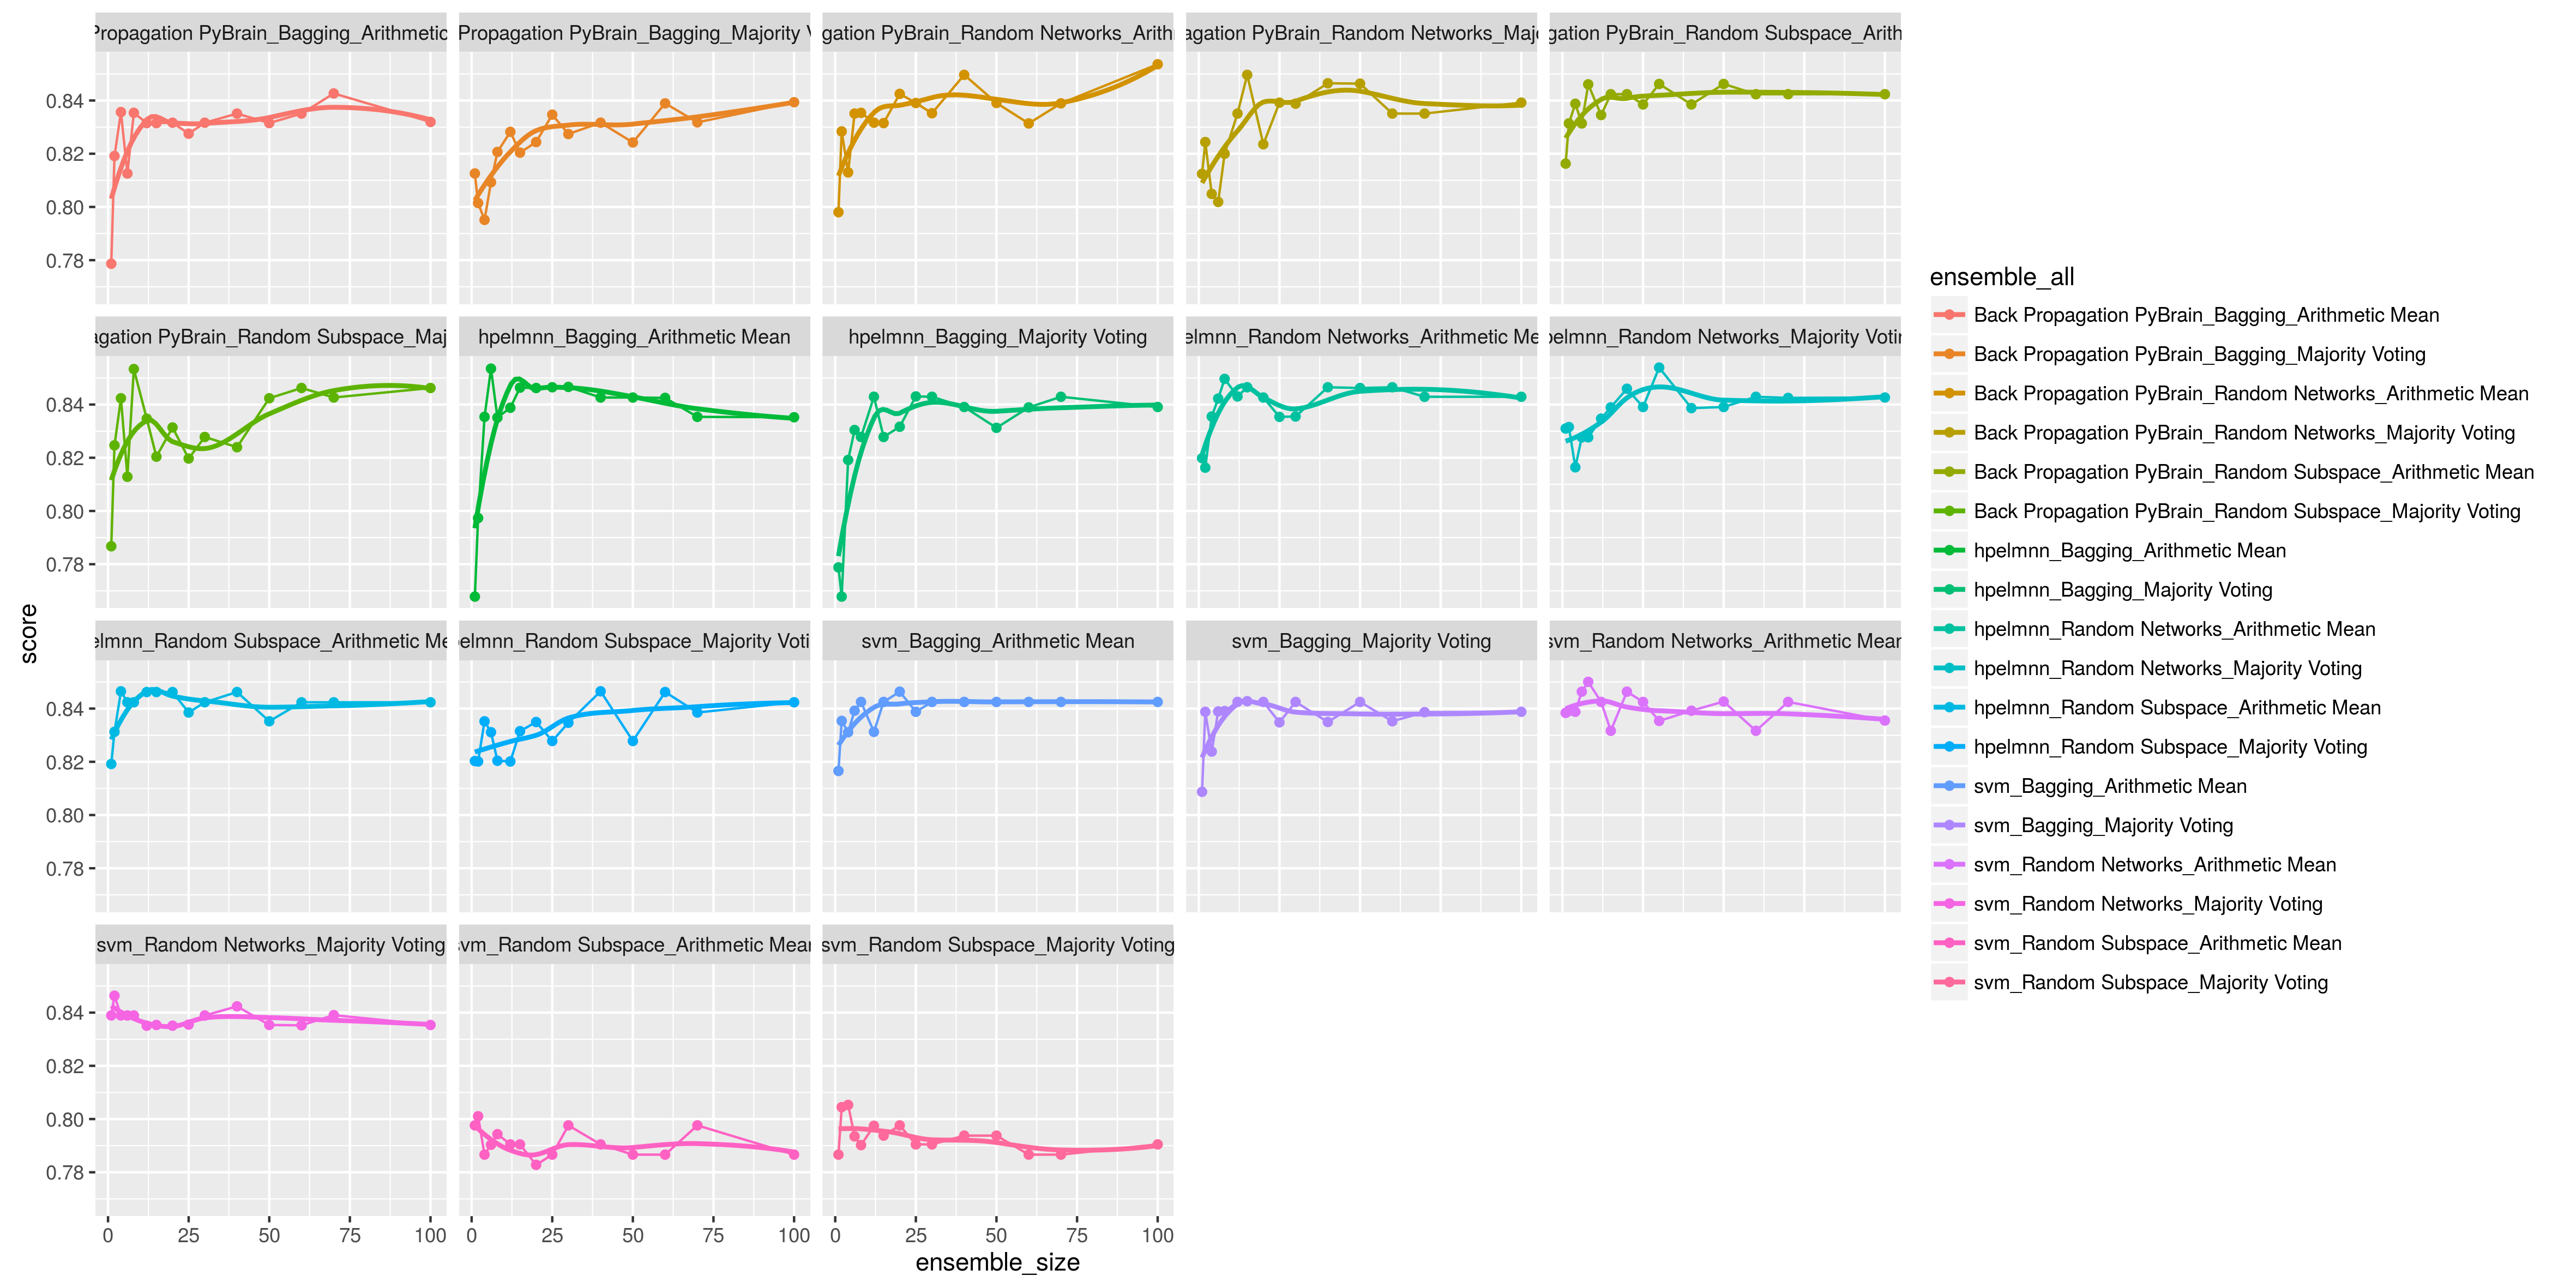
\includegraphics[width=1.0\textwidth]{type2_score_size_model_spect}
    \centering
    \caption{Skuteczność komitetów, \textit{spect} - 22 cechy, 267 obiektów}
    \label{fig:type2_spect}
\end{figure}

\begin{figure}[H]
	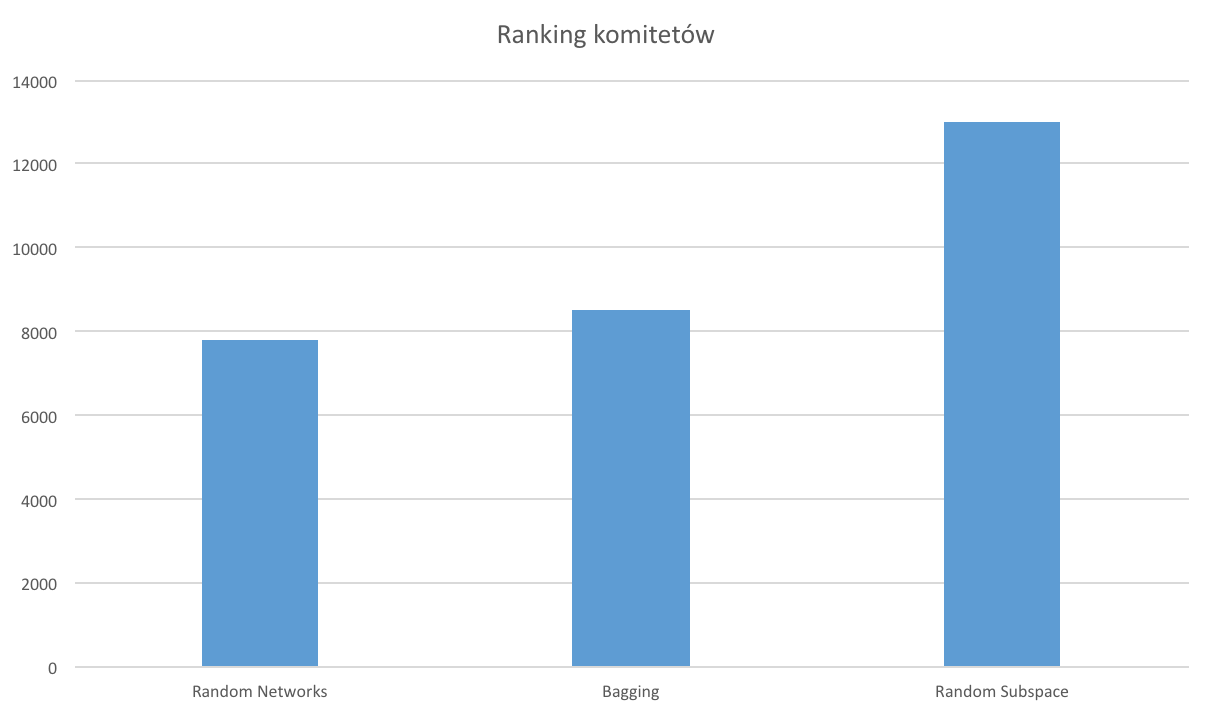
\includegraphics[width=1.0\textwidth]{aggregated_rank_ensemble}
    \centering
    \caption{Wyniki według typu komitetu}
    \label{fig:ensemble_type}
\end{figure}

Na rysunku \ref{fig:ensemble_type} przedstawione zostały zagregowane wyniki uzyskiwane przez poszczególne typy komitetów. Łatwo zauważyć, że w ogólności najlepsze okazało się \textit{Random Networks}, \textit{Bagging} wypadł niewiele gorzej, natomiast \textit{\textit{Random Subspace}} wypadło najgorzej.

\subsection{Random Subspace}
Po przeanalizowaniu wyników komitetu typu \textit{Random Subspace} można stwierdzić, że typ ten nie daje przewagi nad pojedynczą siecią neuronową dla zbiorów obiektów opisanych małą liczbą cech (poniżej 10). Przykłady takich wyników przedstawiono na rysunkach \ref{fig:randomsub_yeast} oraz \ref{fig:randomsub_thyroid}.

\begin{figure}[H]
	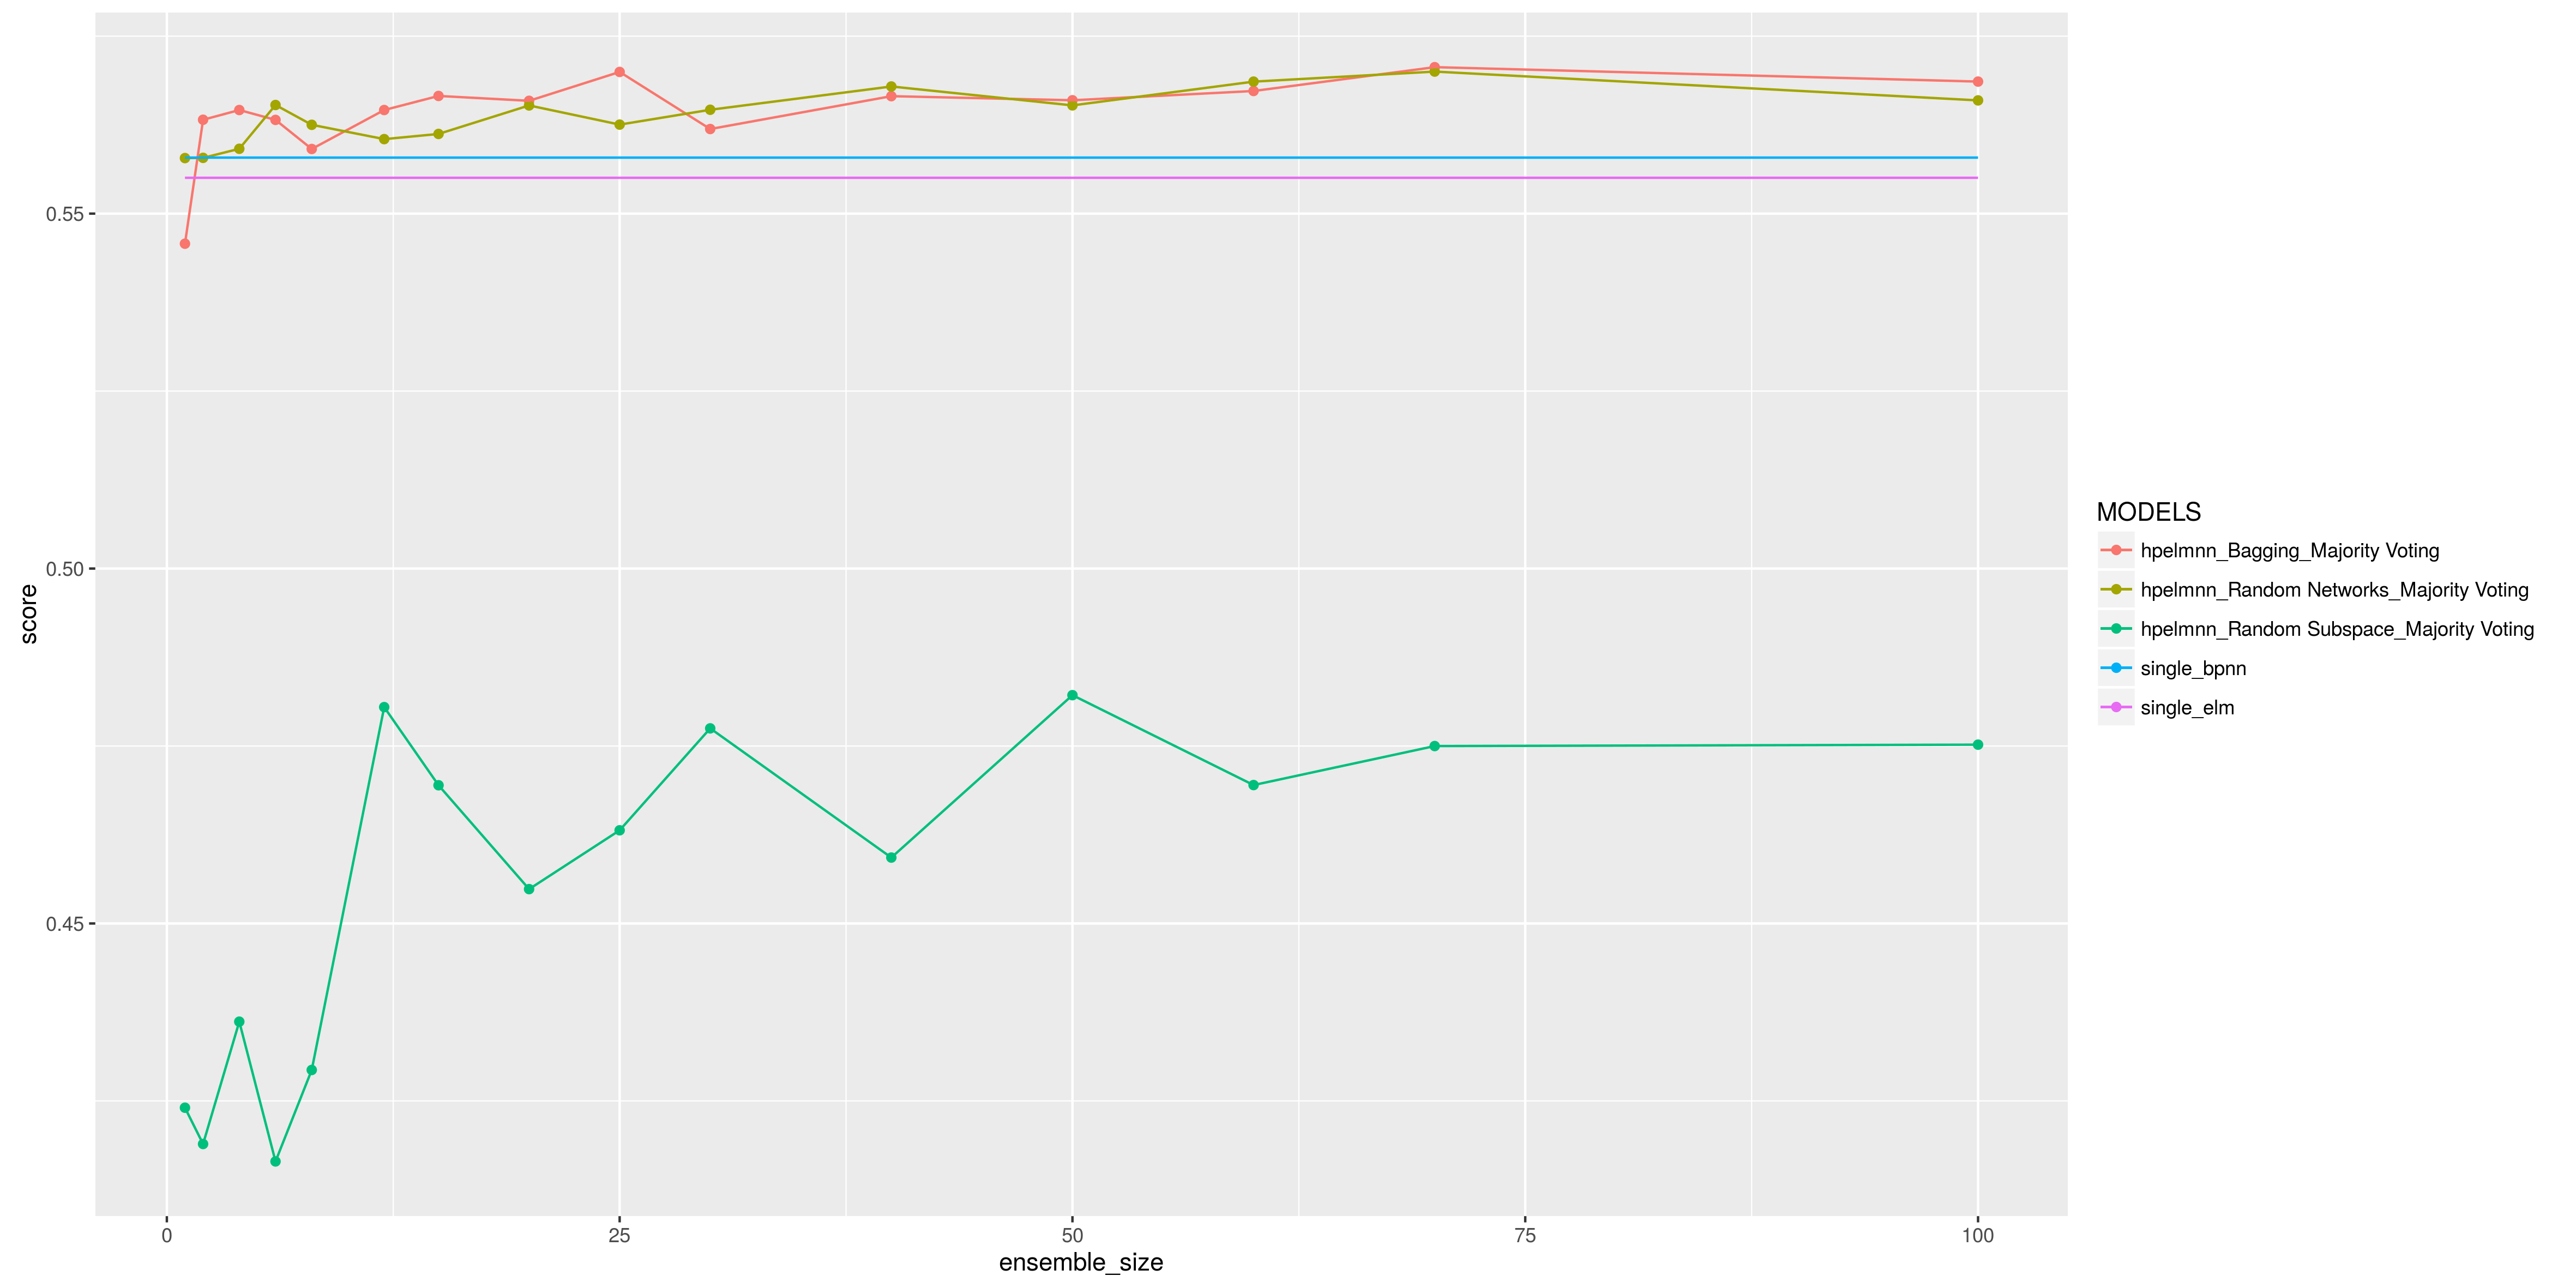
\includegraphics[width=1.0\textwidth]{type4_primary_task_dataset_yeast}
    \centering
    \caption{\textit{yeast} - 8 cech, 1479 obiektów}
    \label{fig:randomsub_yeast}
\end{figure}

\begin{figure}[H]
	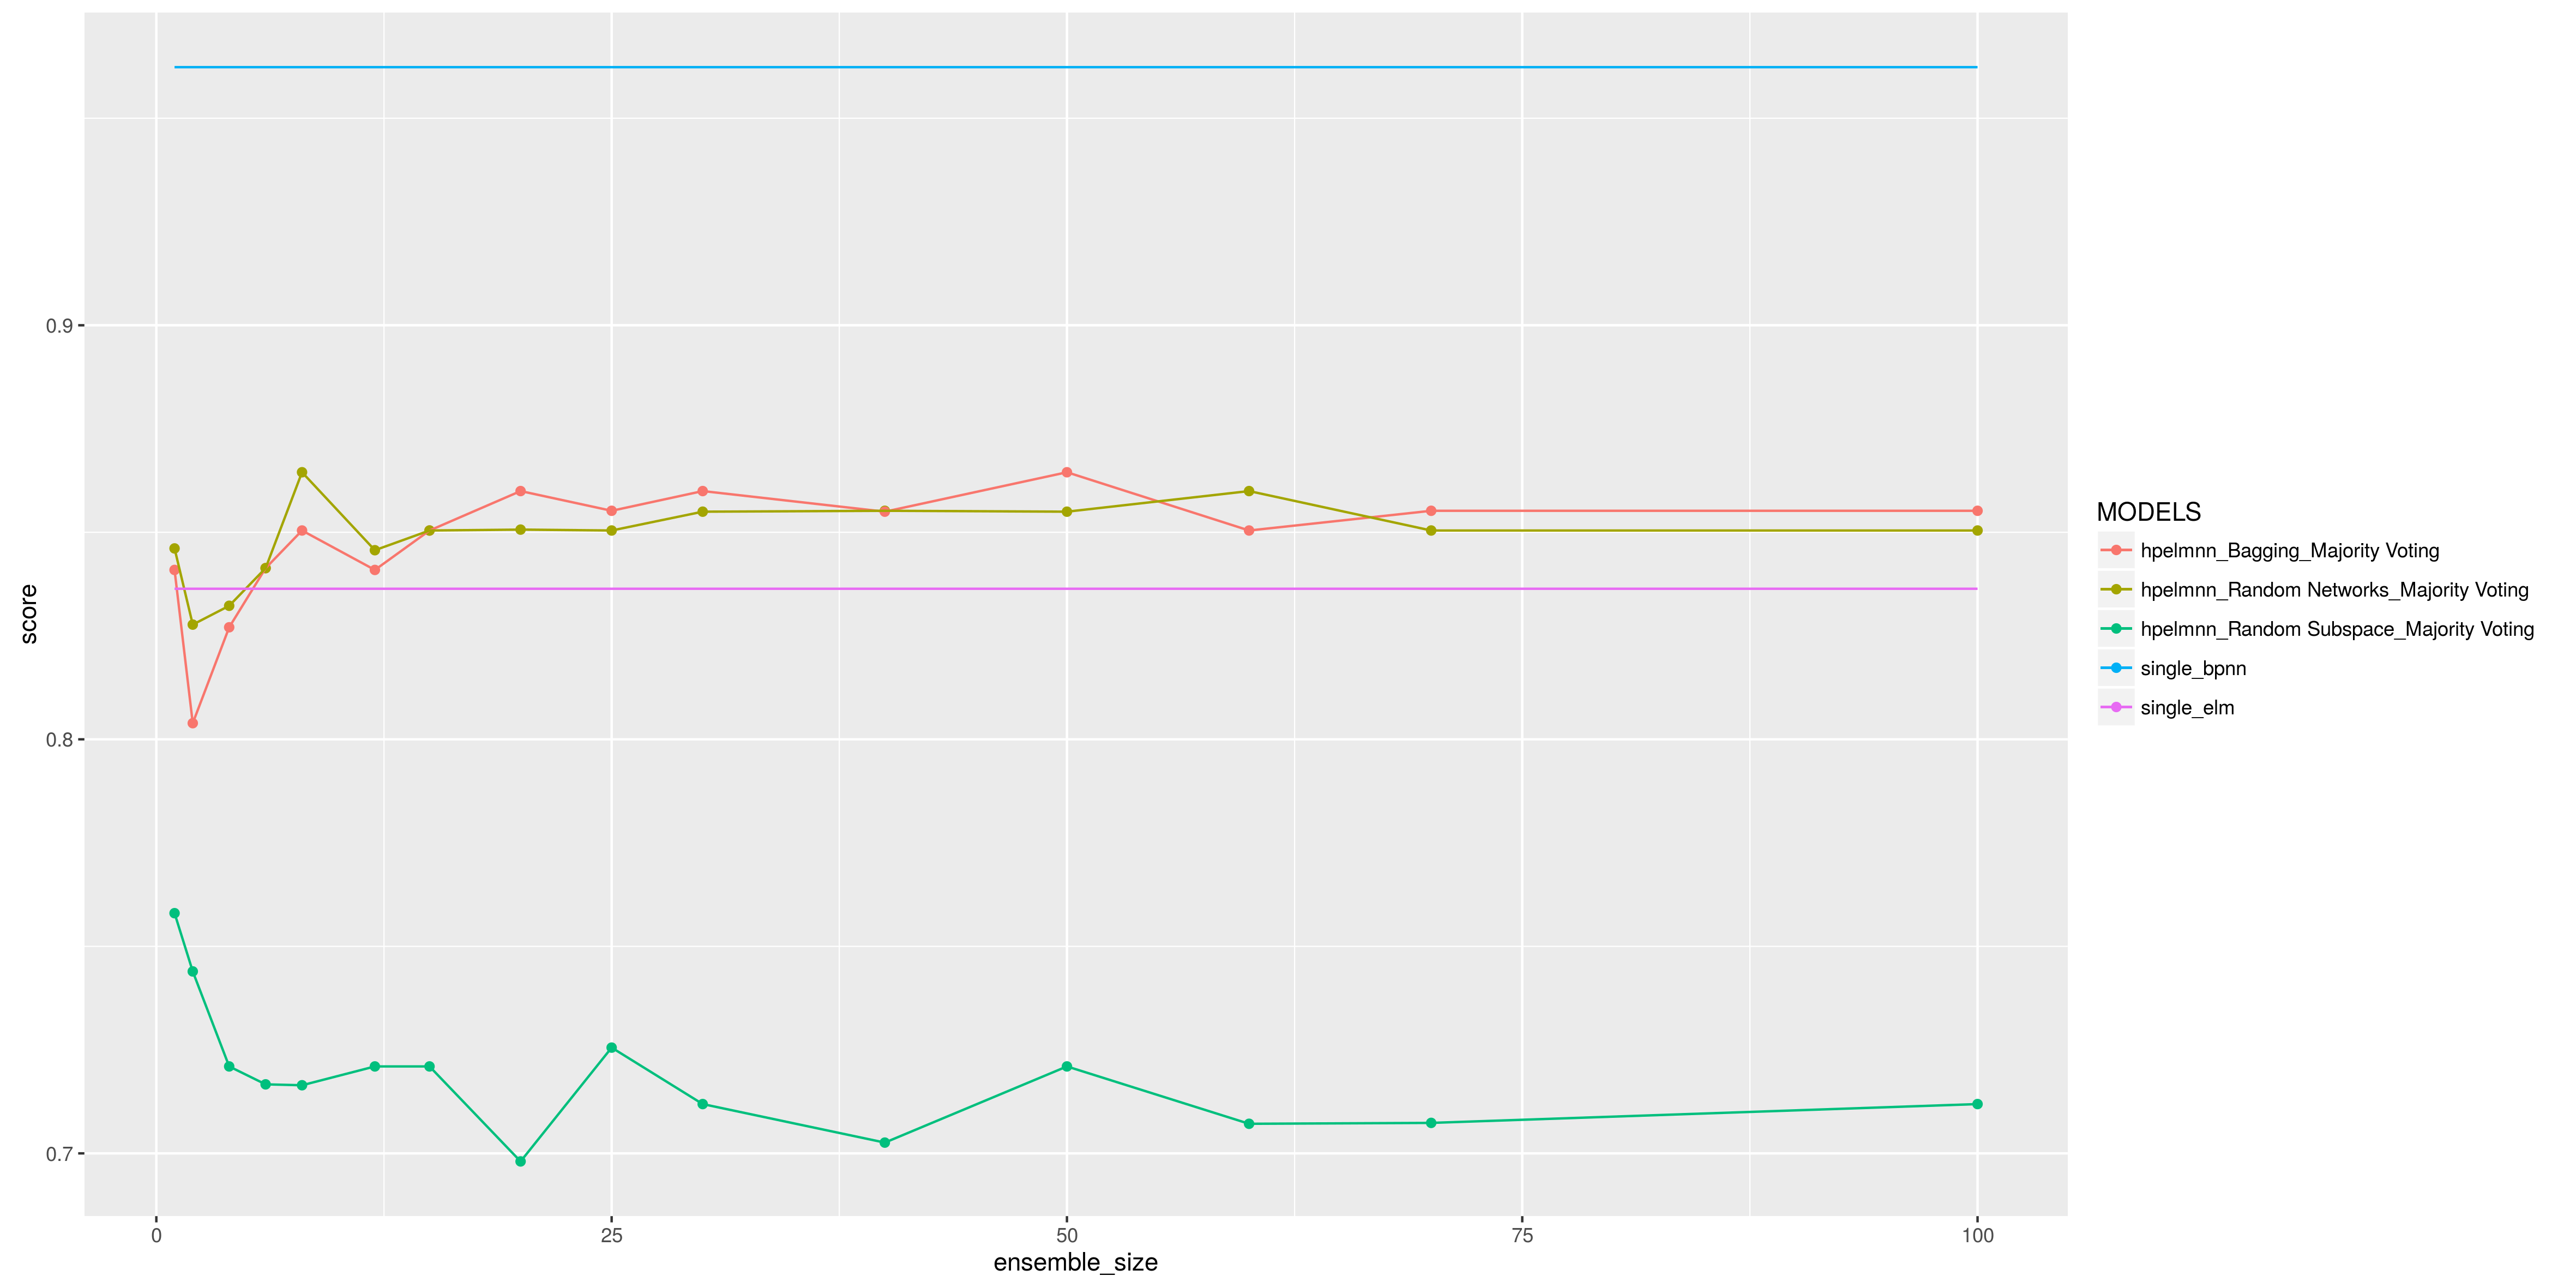
\includegraphics[width=1.0\textwidth]{type4_primary_task_dataset_thyroid}
    \centering
    \caption{\textit{thyroid} - 5 cech, 215 obiektów}
    \label{fig:randomsub_thyroid}
\end{figure}

W przypadku zbiorów danych opisanych większą liczbą cech (w badanych zbiorach wystarczyło już kilkanaście cech) oraz rozmiaru komitetu większego niż 10, komitet ten był porównywalny z innymi typami komitetów, a także okazał się lepszy od pojedynczego klasyfikatora. Przykłady wyników dla takich zbiorów przedstawiają rysunki \ref{fig:randomsub_dermatology} i \ref{fig:randomsub_urban_land_cover}.

Taki wynik badań był łatwy do przewidzenia. W przypadku małej liczby cech, podzbiór wylosowany do trenowania klasyfikatorów bazowych jest niewystarczający do poprawnego klasyfikowania obiektów testowych. W przypadku dużej liczby cech sytuacja zmienia się i zróżnicowanie znanych przez modele bazowe cech zwiększa generalizację sieci poprawiając tym samym jej skuteczność.

\begin{figure}[H]
	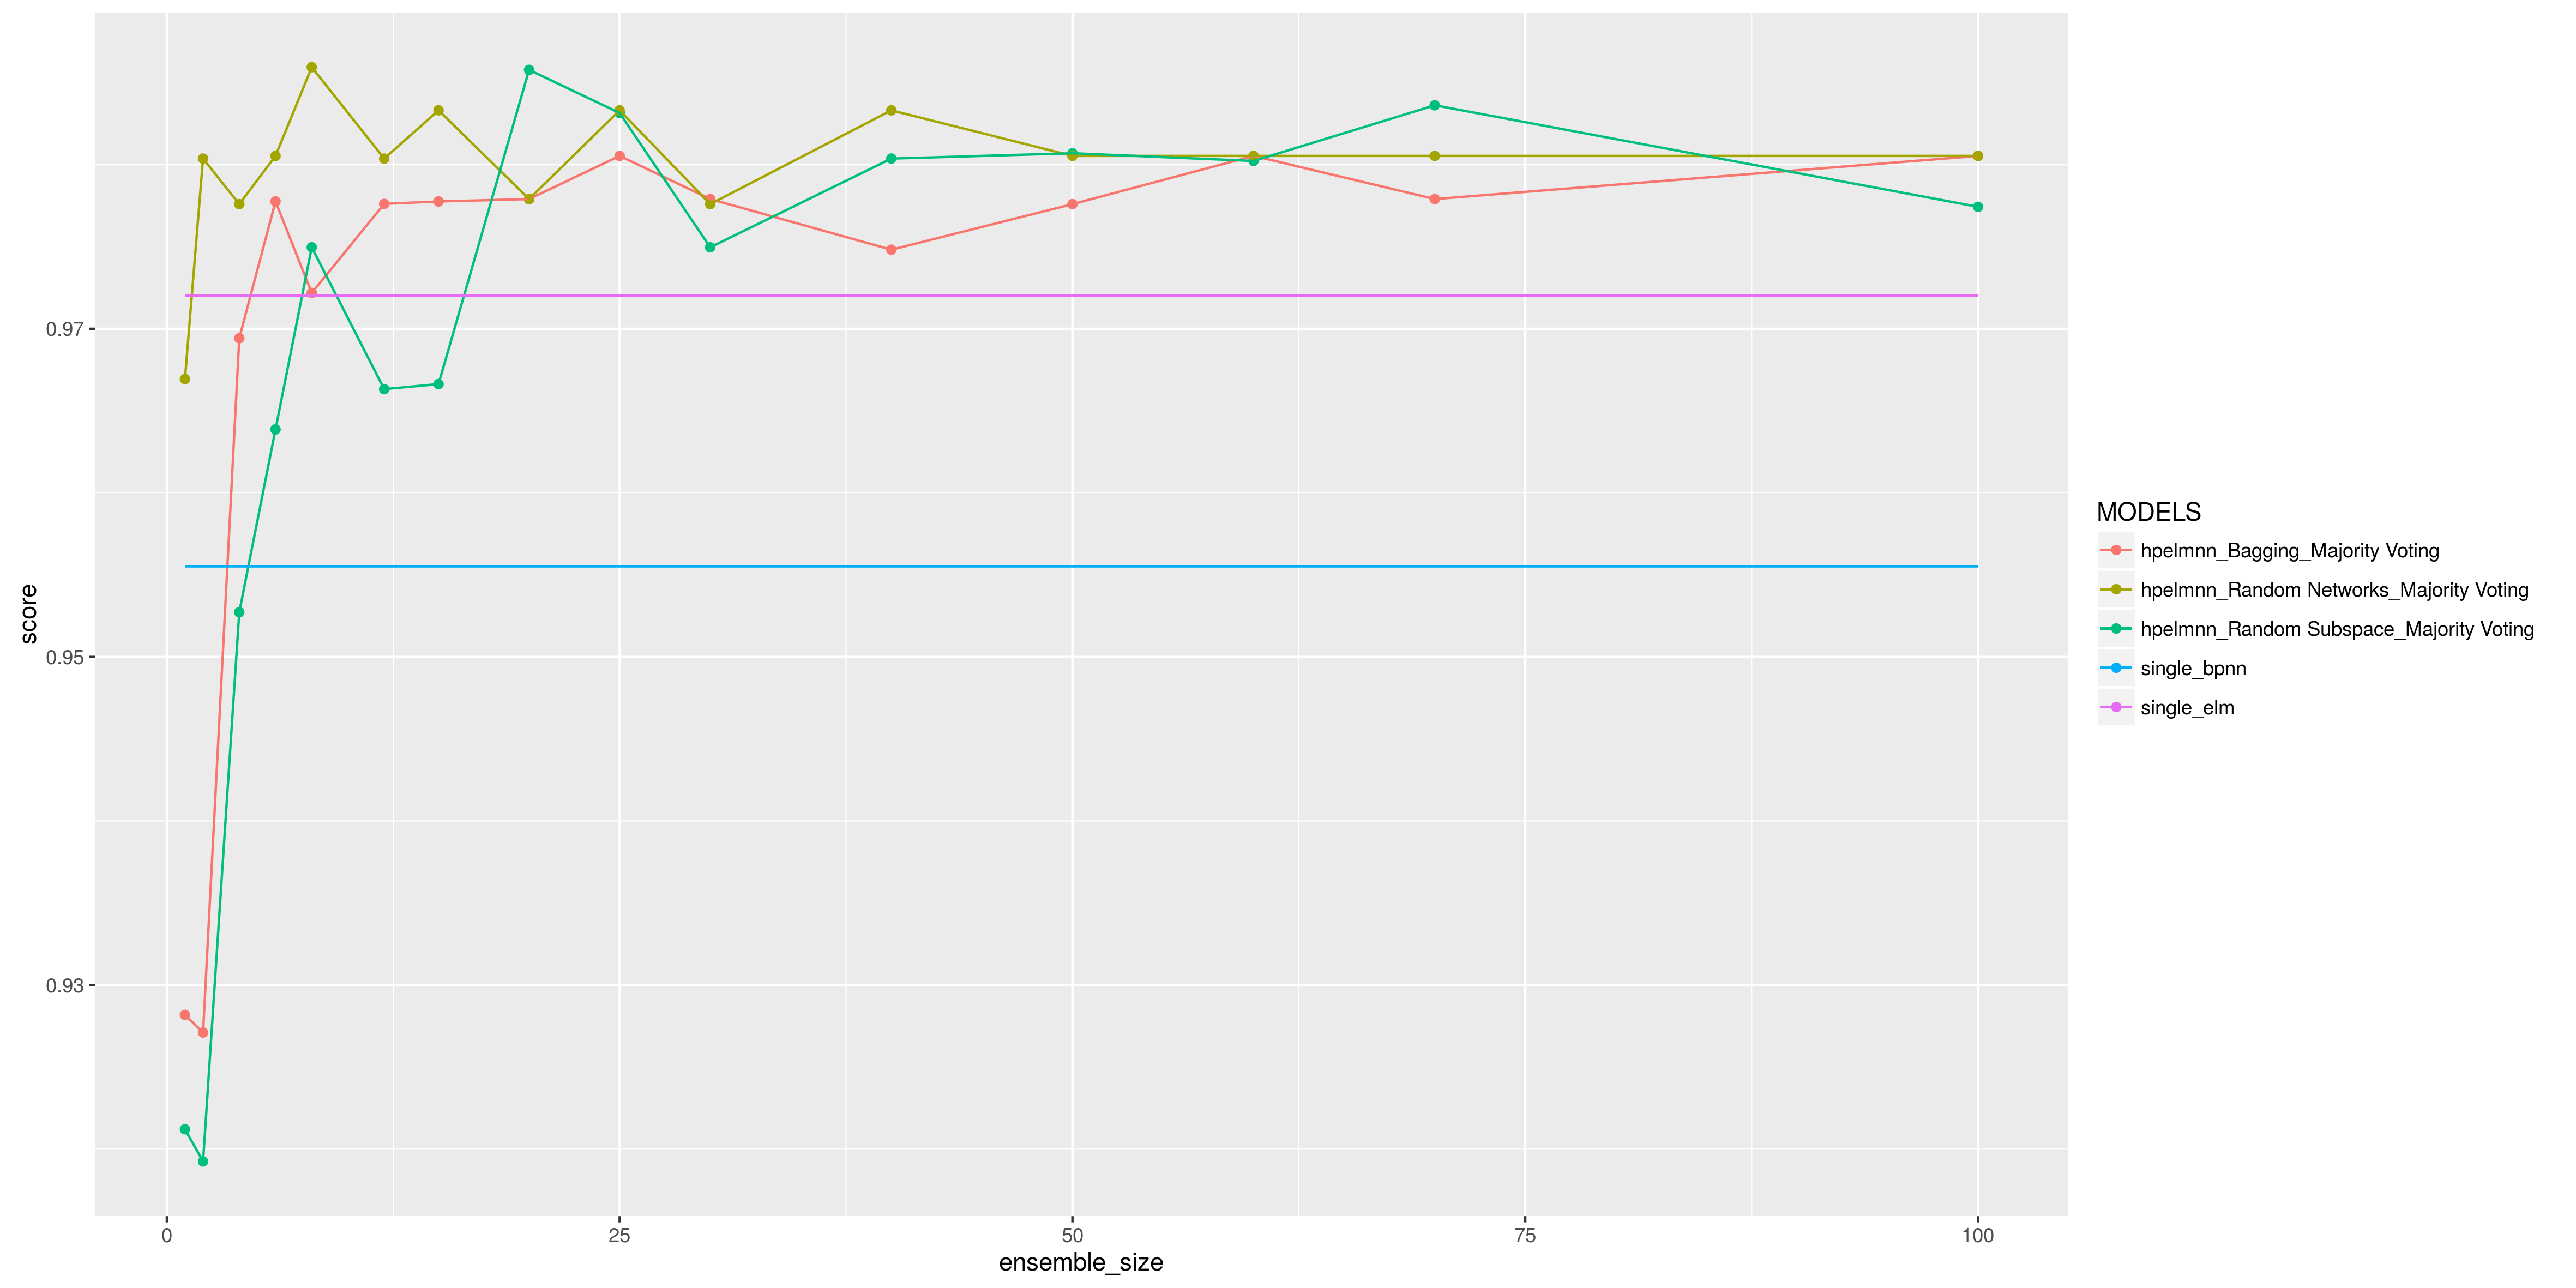
\includegraphics[width=1.0\textwidth]{type4_primary_task_dataset_dermatology}
    \centering
    \caption{\textit{dermatology} - 34 cechy, 358 obiektów}
    \label{fig:randomsub_dermatology}
\end{figure}

\begin{figure}[H]
	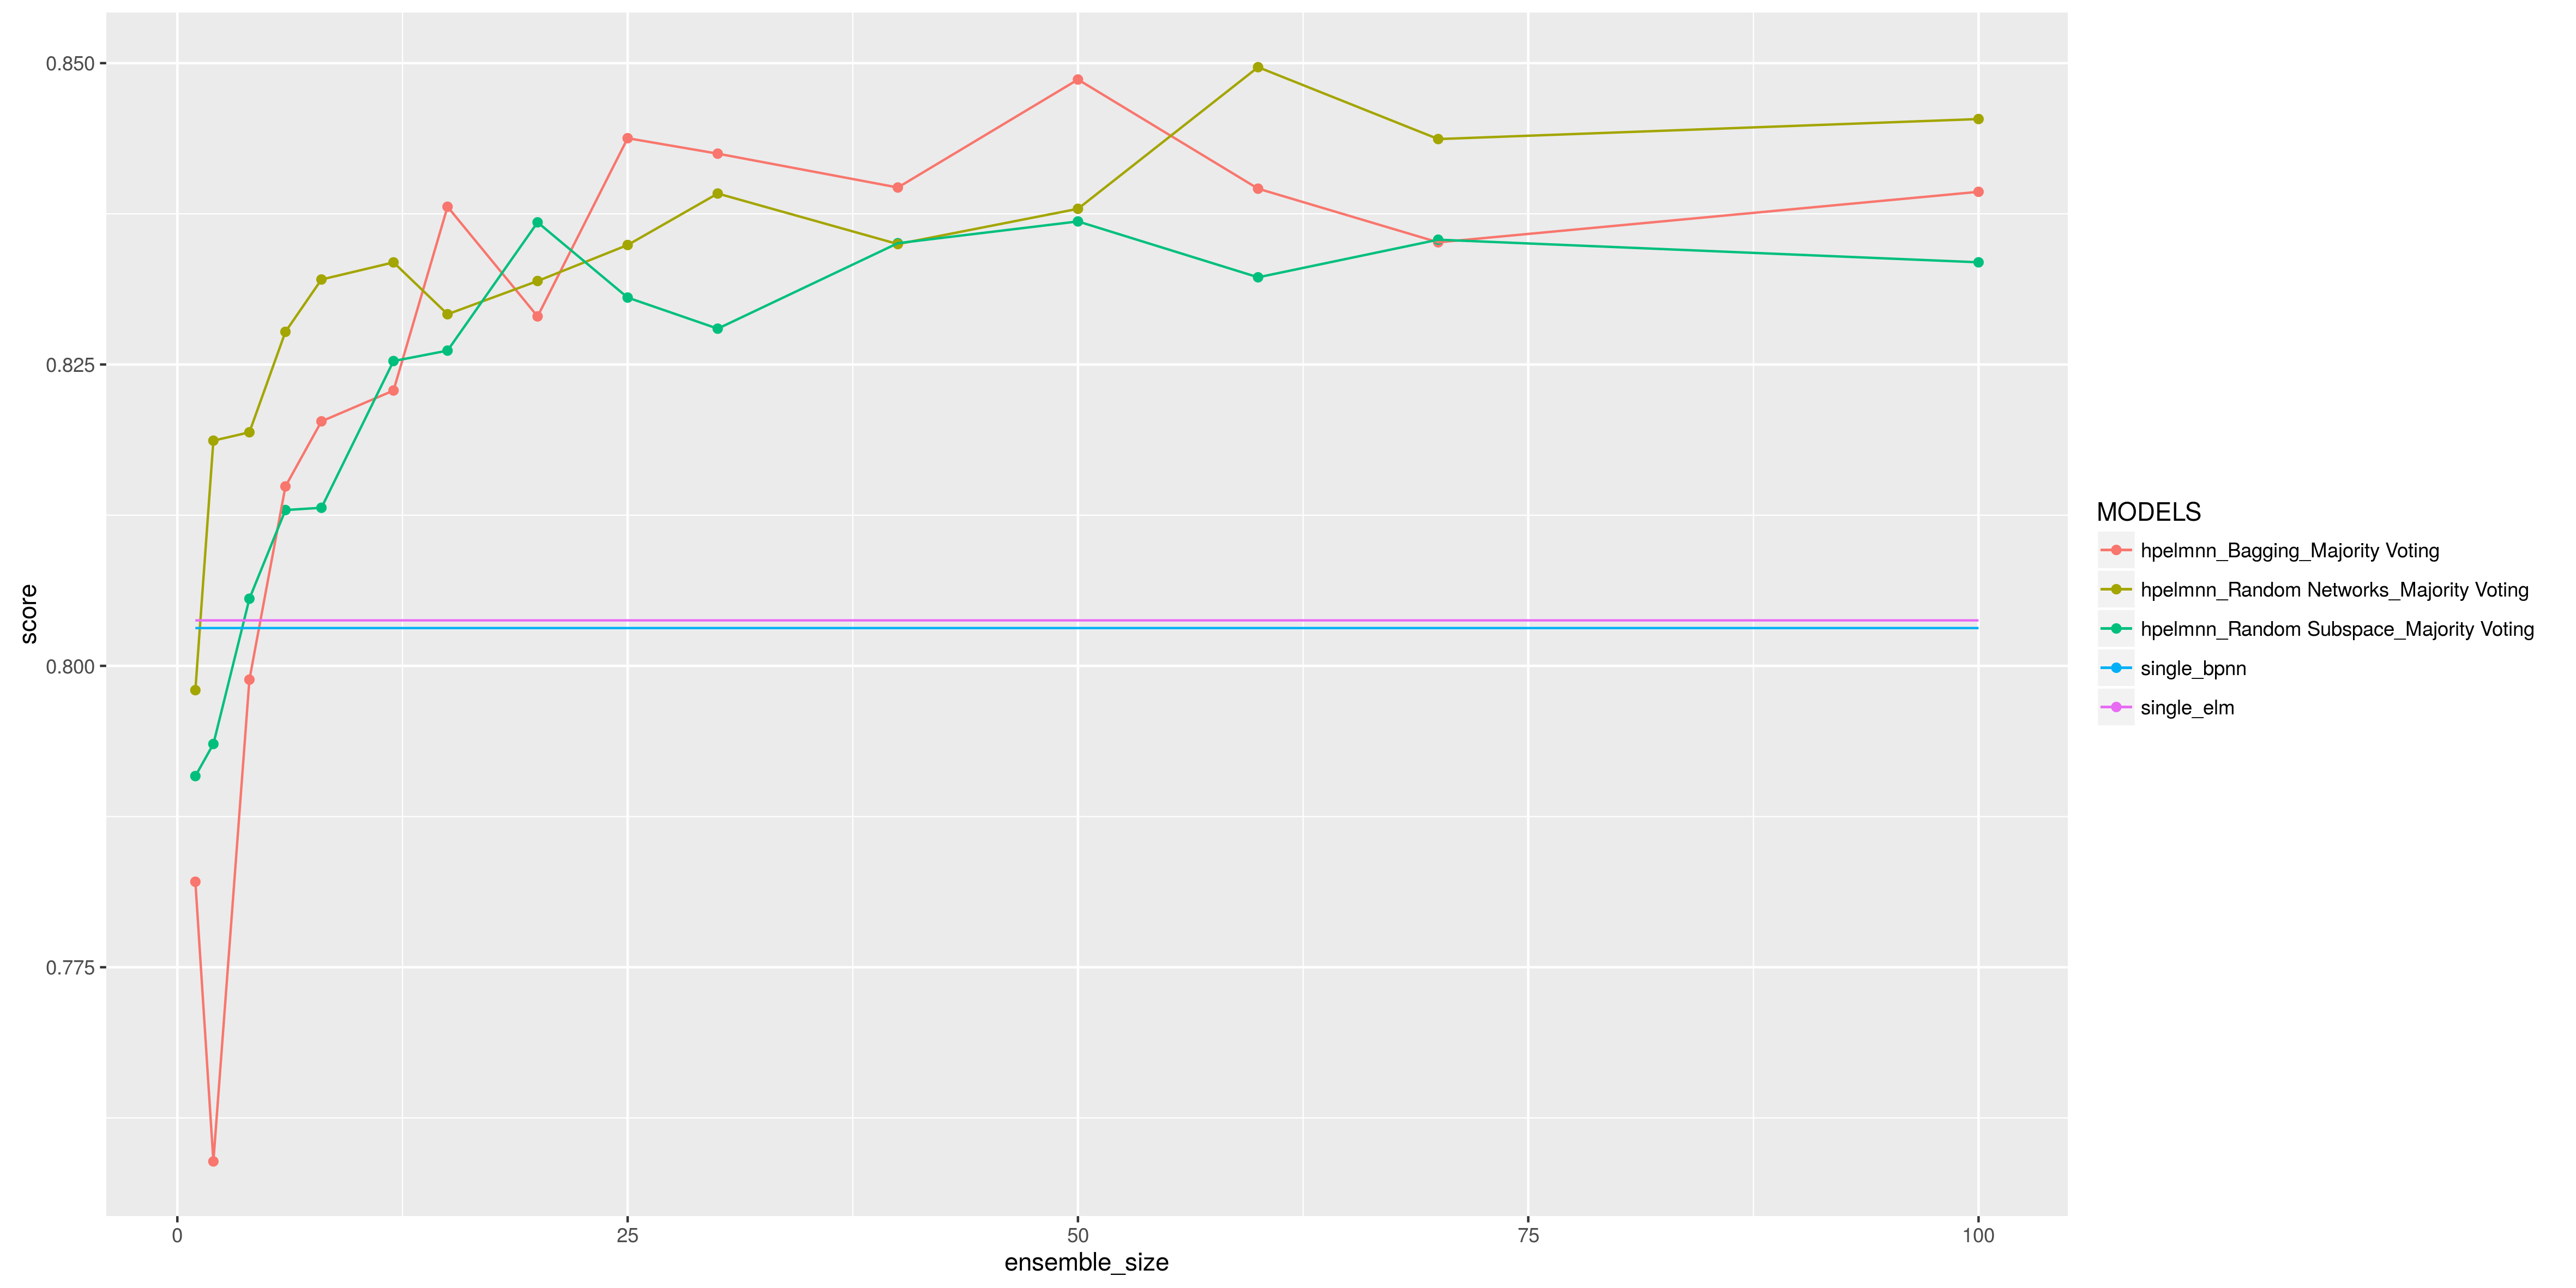
\includegraphics[width=1.0\textwidth]{type4_primary_task_dataset_urban_land_cover}
    \centering
    \caption{\textit{urban\_land} - 147 cech, 675 obiektów}
    \label{fig:randomsub_urban_land_cover}
\end{figure}

\subsection{Bagging}

Skuteczności uzyskiwane przez \textit{Bagging} (rysunek \ref{fig:ensemble_type}) są stosunkowo dobre. Nie został zaobserwowany żaden szczególny wpływ liczby cech lub obiektów uczących na rezultaty.

\begin{figure}[H]
	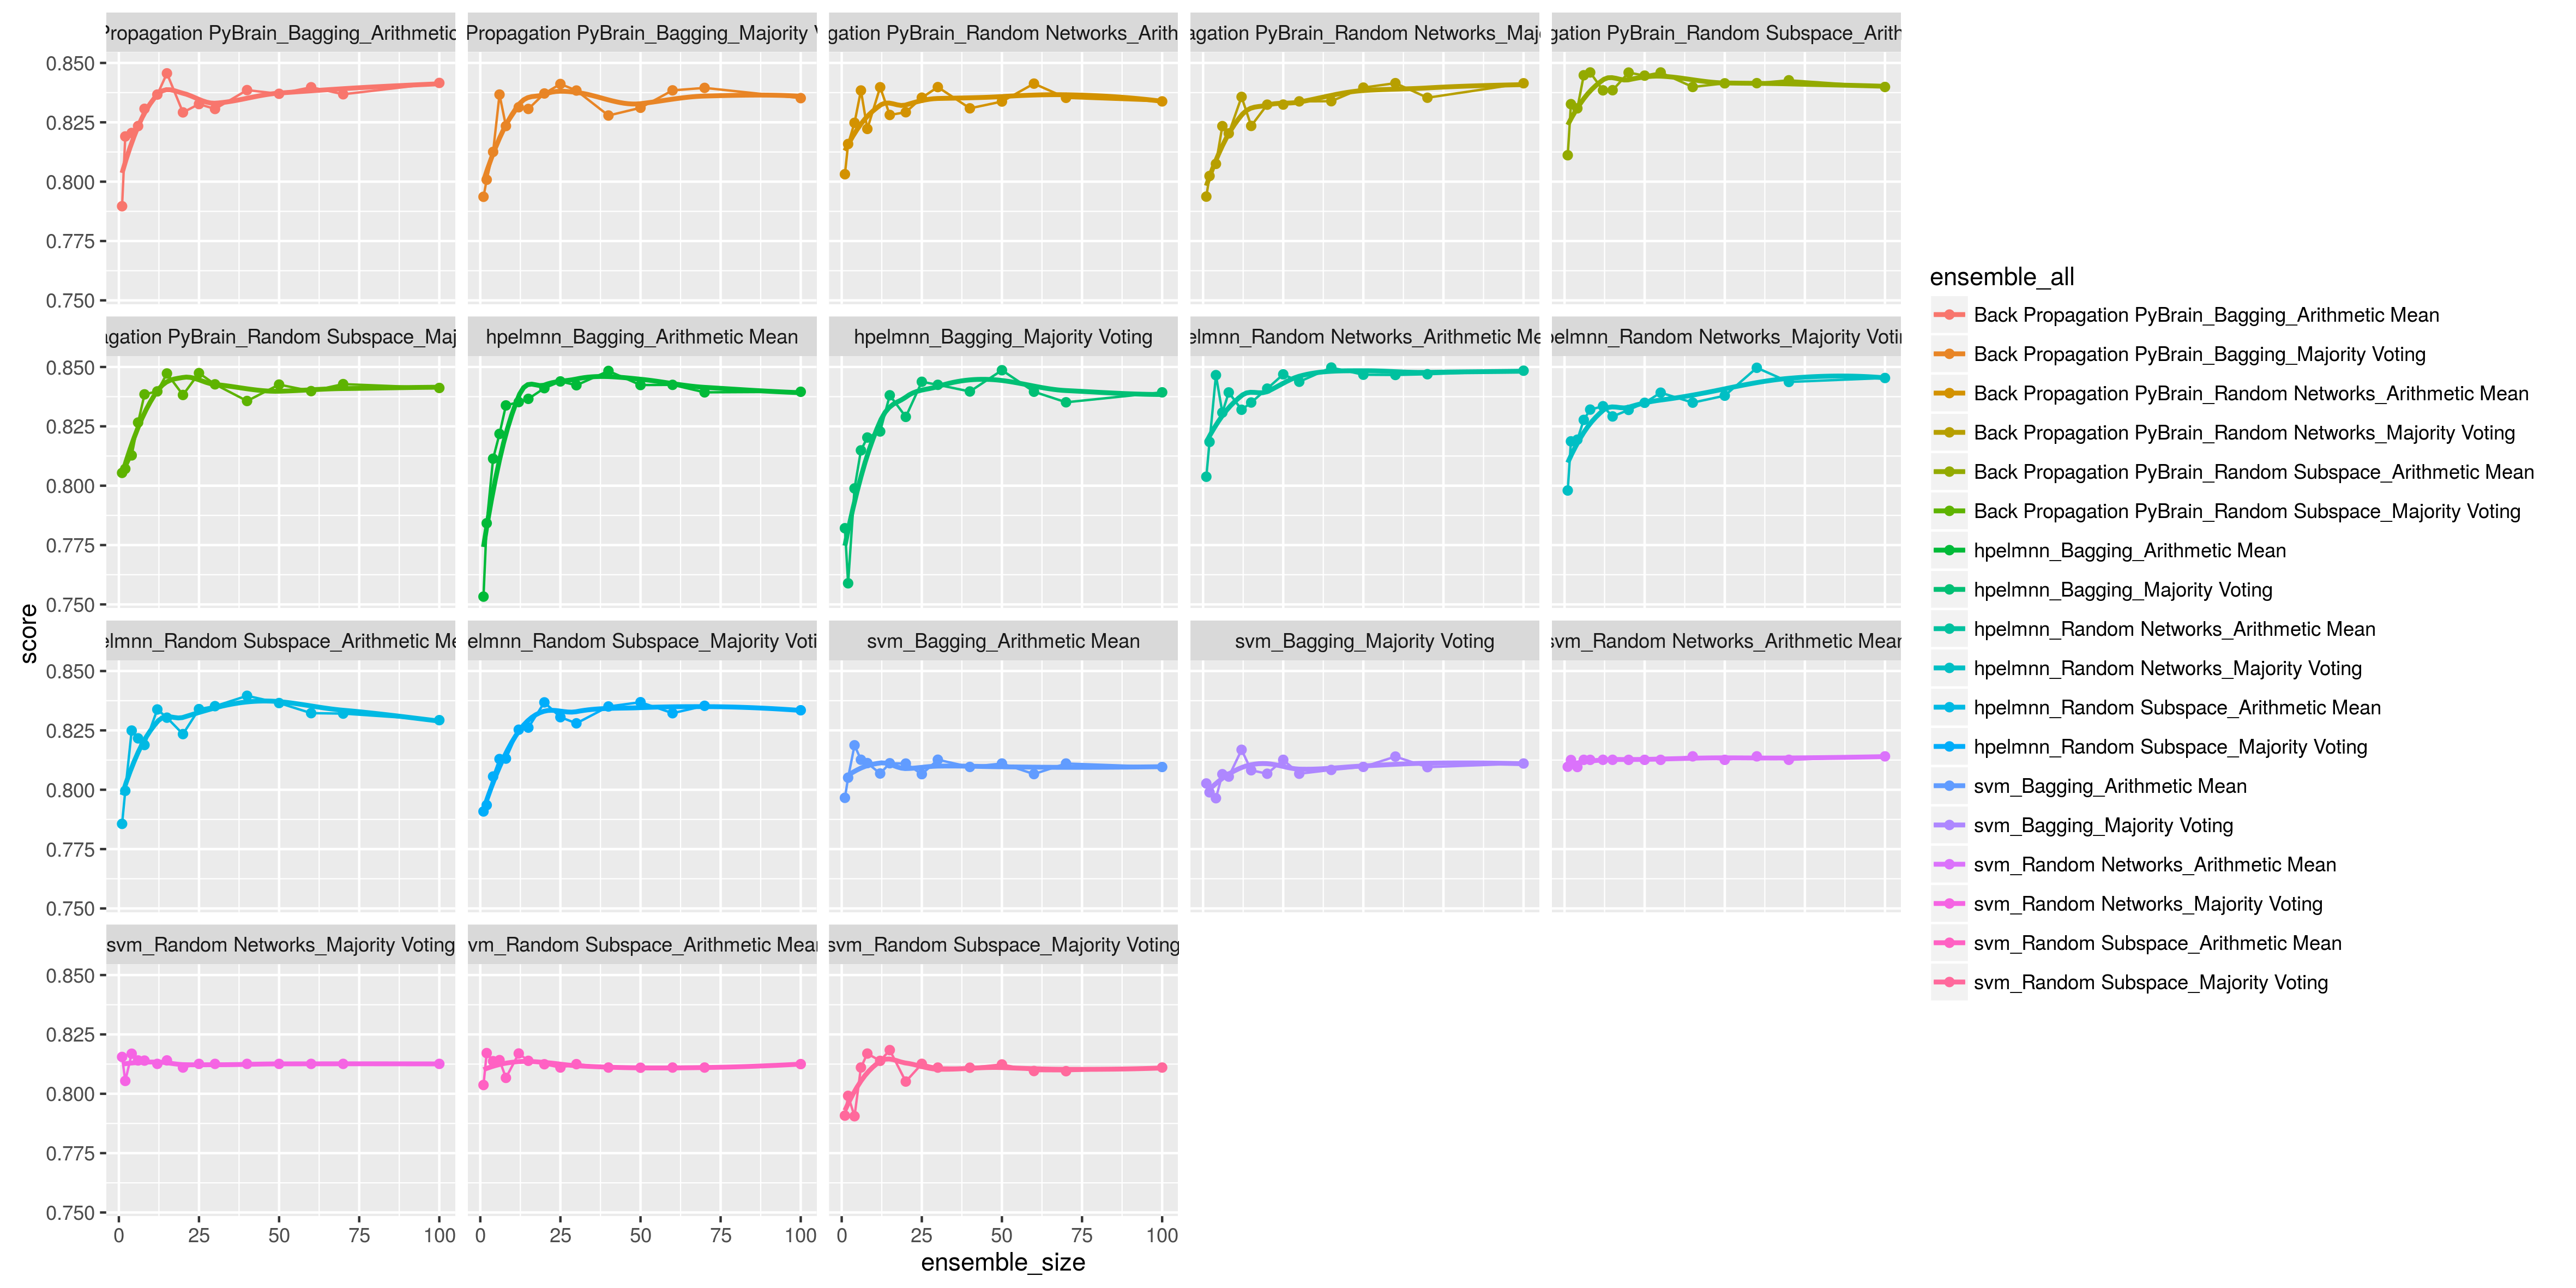
\includegraphics[width=1.0\textwidth]{type2_score_size_model_urban_land_cover}
    \centering
    \caption{\textit{urban\_land} - 147 cech, 675 obiektów}
    \label{fig:type2_urban_land_cover}
\end{figure}

Na rysunku \ref{fig:type2_urban_land_cover} można zaobserwować,jak zmieniała się skuteczność wraz ze zmianą liczby członków. Na początku jakość klasyfikacji zwiększa się szybko, osiąga ekstremum najczęściej w okolicach rozmiaru 15-25. Następnie stabilizuje się i dalsze dodawanie klasyfikatorów nie wpływa już znacząco na wyniki.

\subsection{Random Networks}

W naszych badaniach komitety typu \textit{Random Networks} okazały się najskuteczniejsze. Zjawisko to można próbować tłumaczyć tym, że ten sposób budowy komitetów w żaden sposób nie zmniejsza skuteczności działania indywidualnych klasyfikatorów. W przypadku podziału zbioru danych tak jak w \textit{Random Subspace} czy \textit{Bagging}u, część danych jest faktycznie przed pojedynczym klasyfikatorem ukrywana. Można więc stwierdzić, że w zastosowanych przez nas zbiorach danych i komitetach czynnikiem istotniejszym od różnorodności pojedynczego klasyfikatora okazała się skuteczność.

Warto także zwrócić uwagę na fakt, że skuteczność komitetów typu \textit{Random Networks} w mniejszym stopniu zależy od rozmiaru badanych komitetów. Sytuacja została zobrazowana na wykresie \ref{fig:type2_yeast}. Wpływ na takie zjawisko ma fakt, że poszczególne elementy komitetu Random Networks są uczone na całym zbiorze uczącym, przez co pojedynczy klasyfikator powinien byc bardziej skuteczny niż w metodach Random Subspace i Bagging.

\begin{figure}[H]
	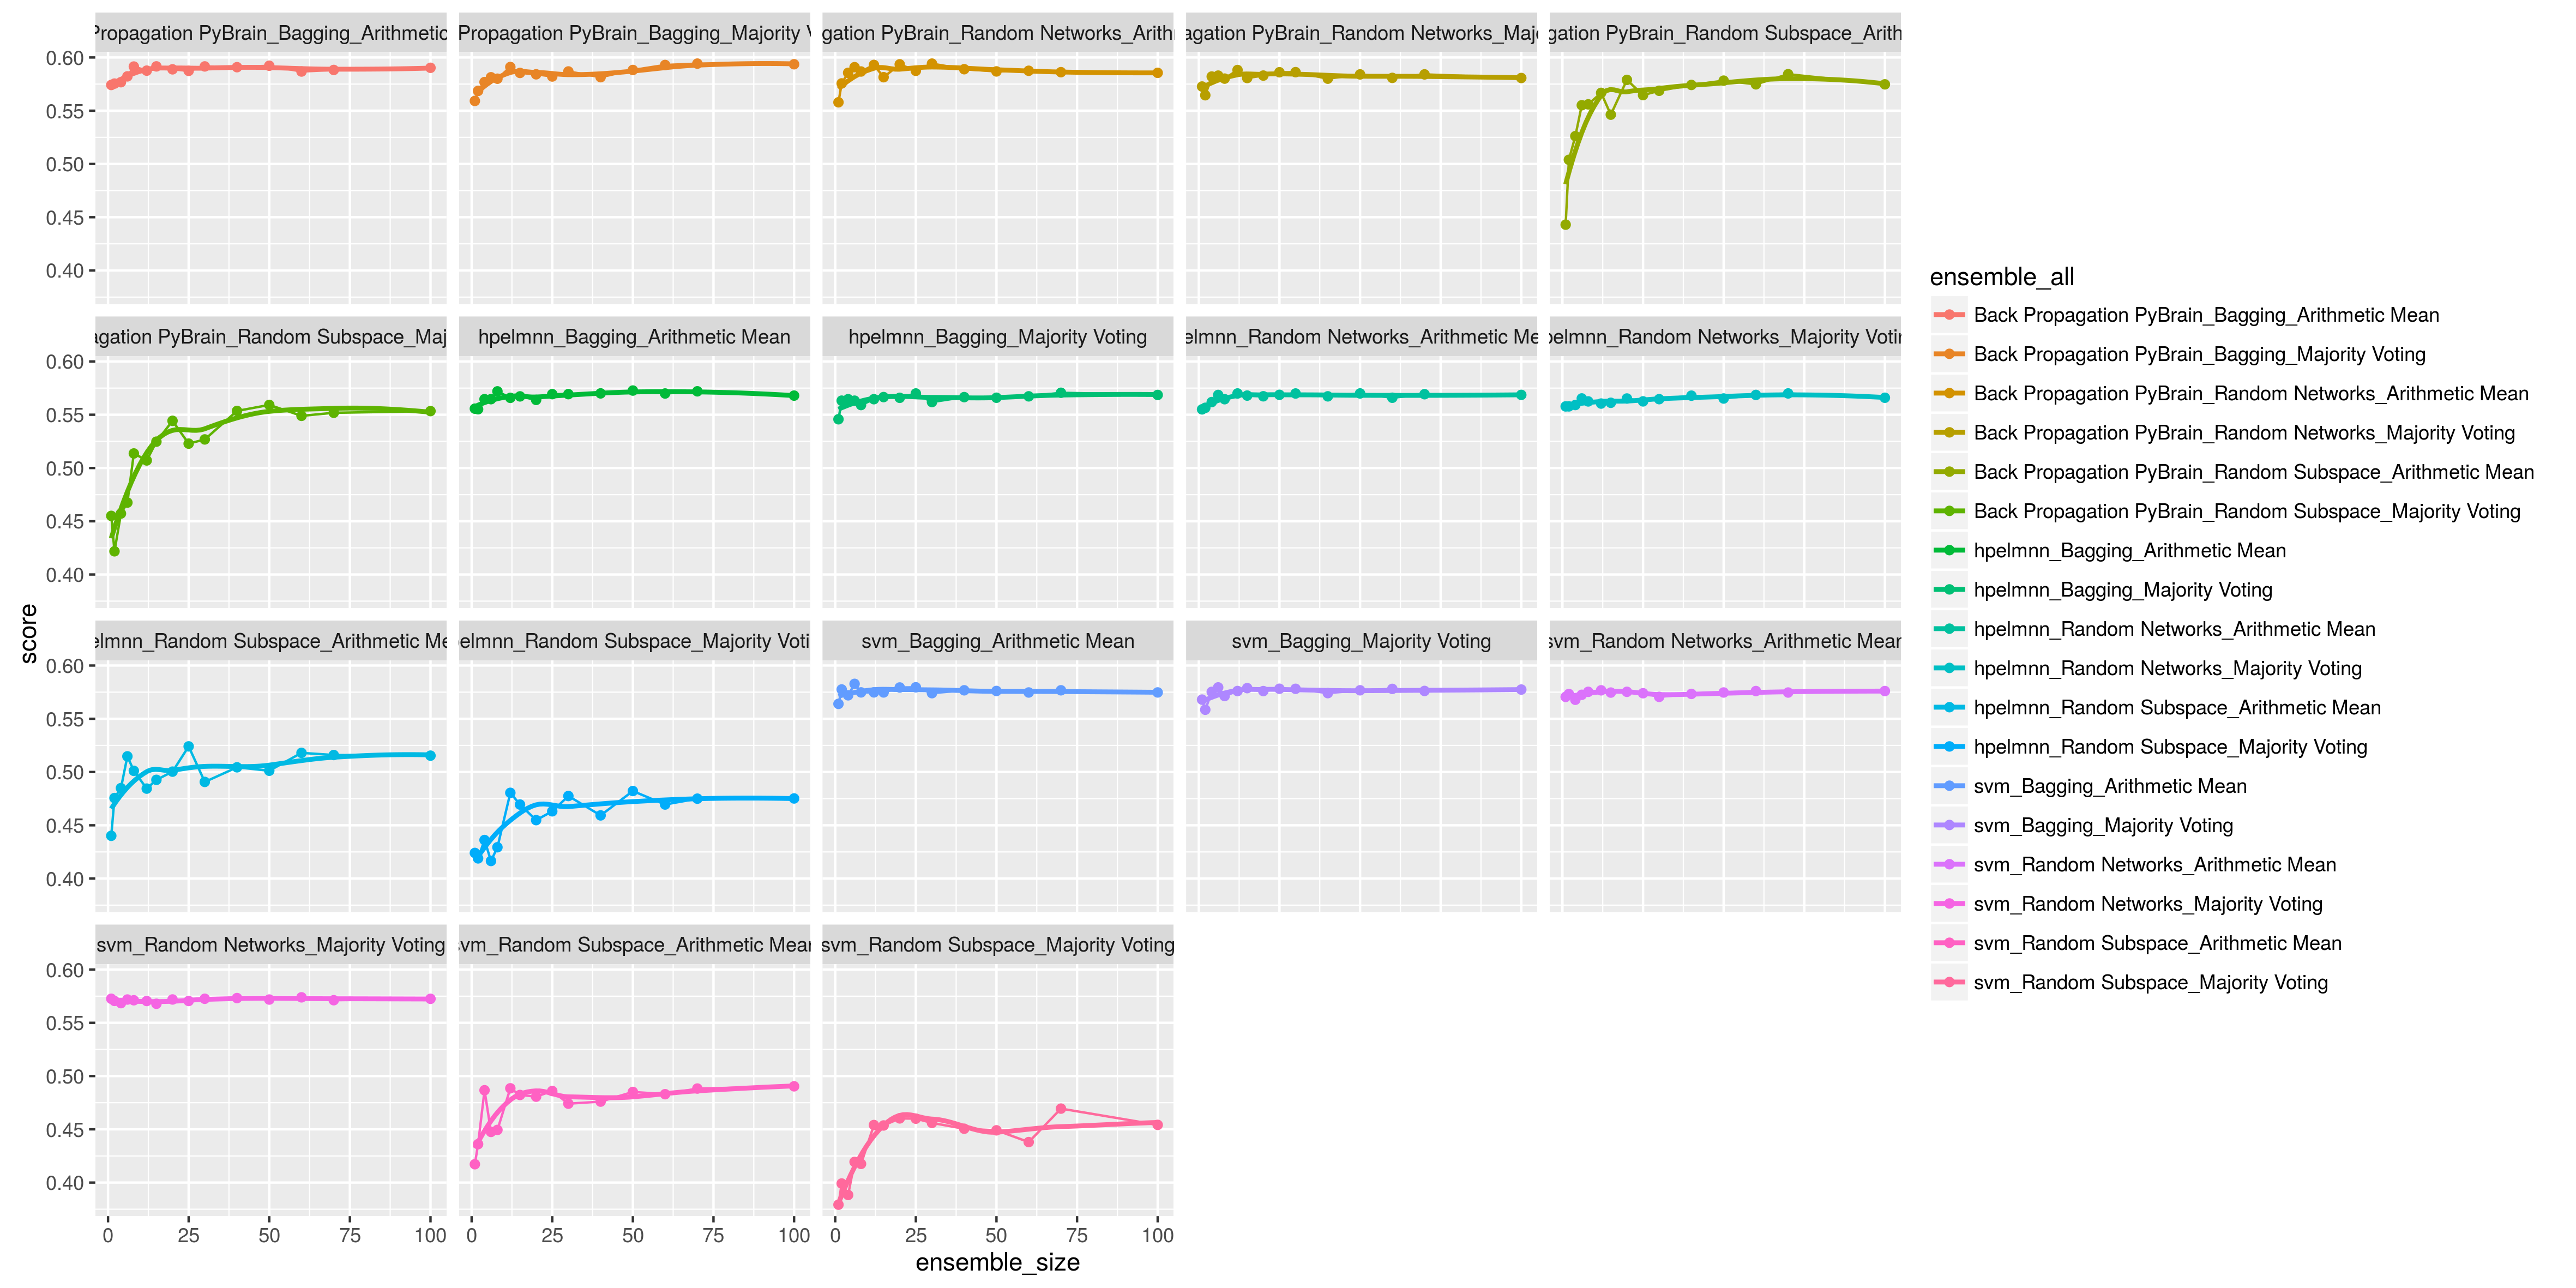
\includegraphics[width=1.0\textwidth]{type2_score_size_model_yeast}
    \centering
    \caption{Wyniki skuteczności wszystkich typów komitetów na zbiorze \textit{yeast}}
    \label{fig:type2_yeast}
\end{figure}

W większości przeanalizowanych zestawów danych maksymalna skuteczność komitetu Random Networks jest osiągana przy rozmiarze 8-12 modeli. Przy zwiększeniu liczby członków powyżej 12 nie ma już zauważalnego wzrostu skuteczności, co zostało zobrazowane na wykresie \ref{fig:type2_dermatology}. 

\begin{figure}[H]
	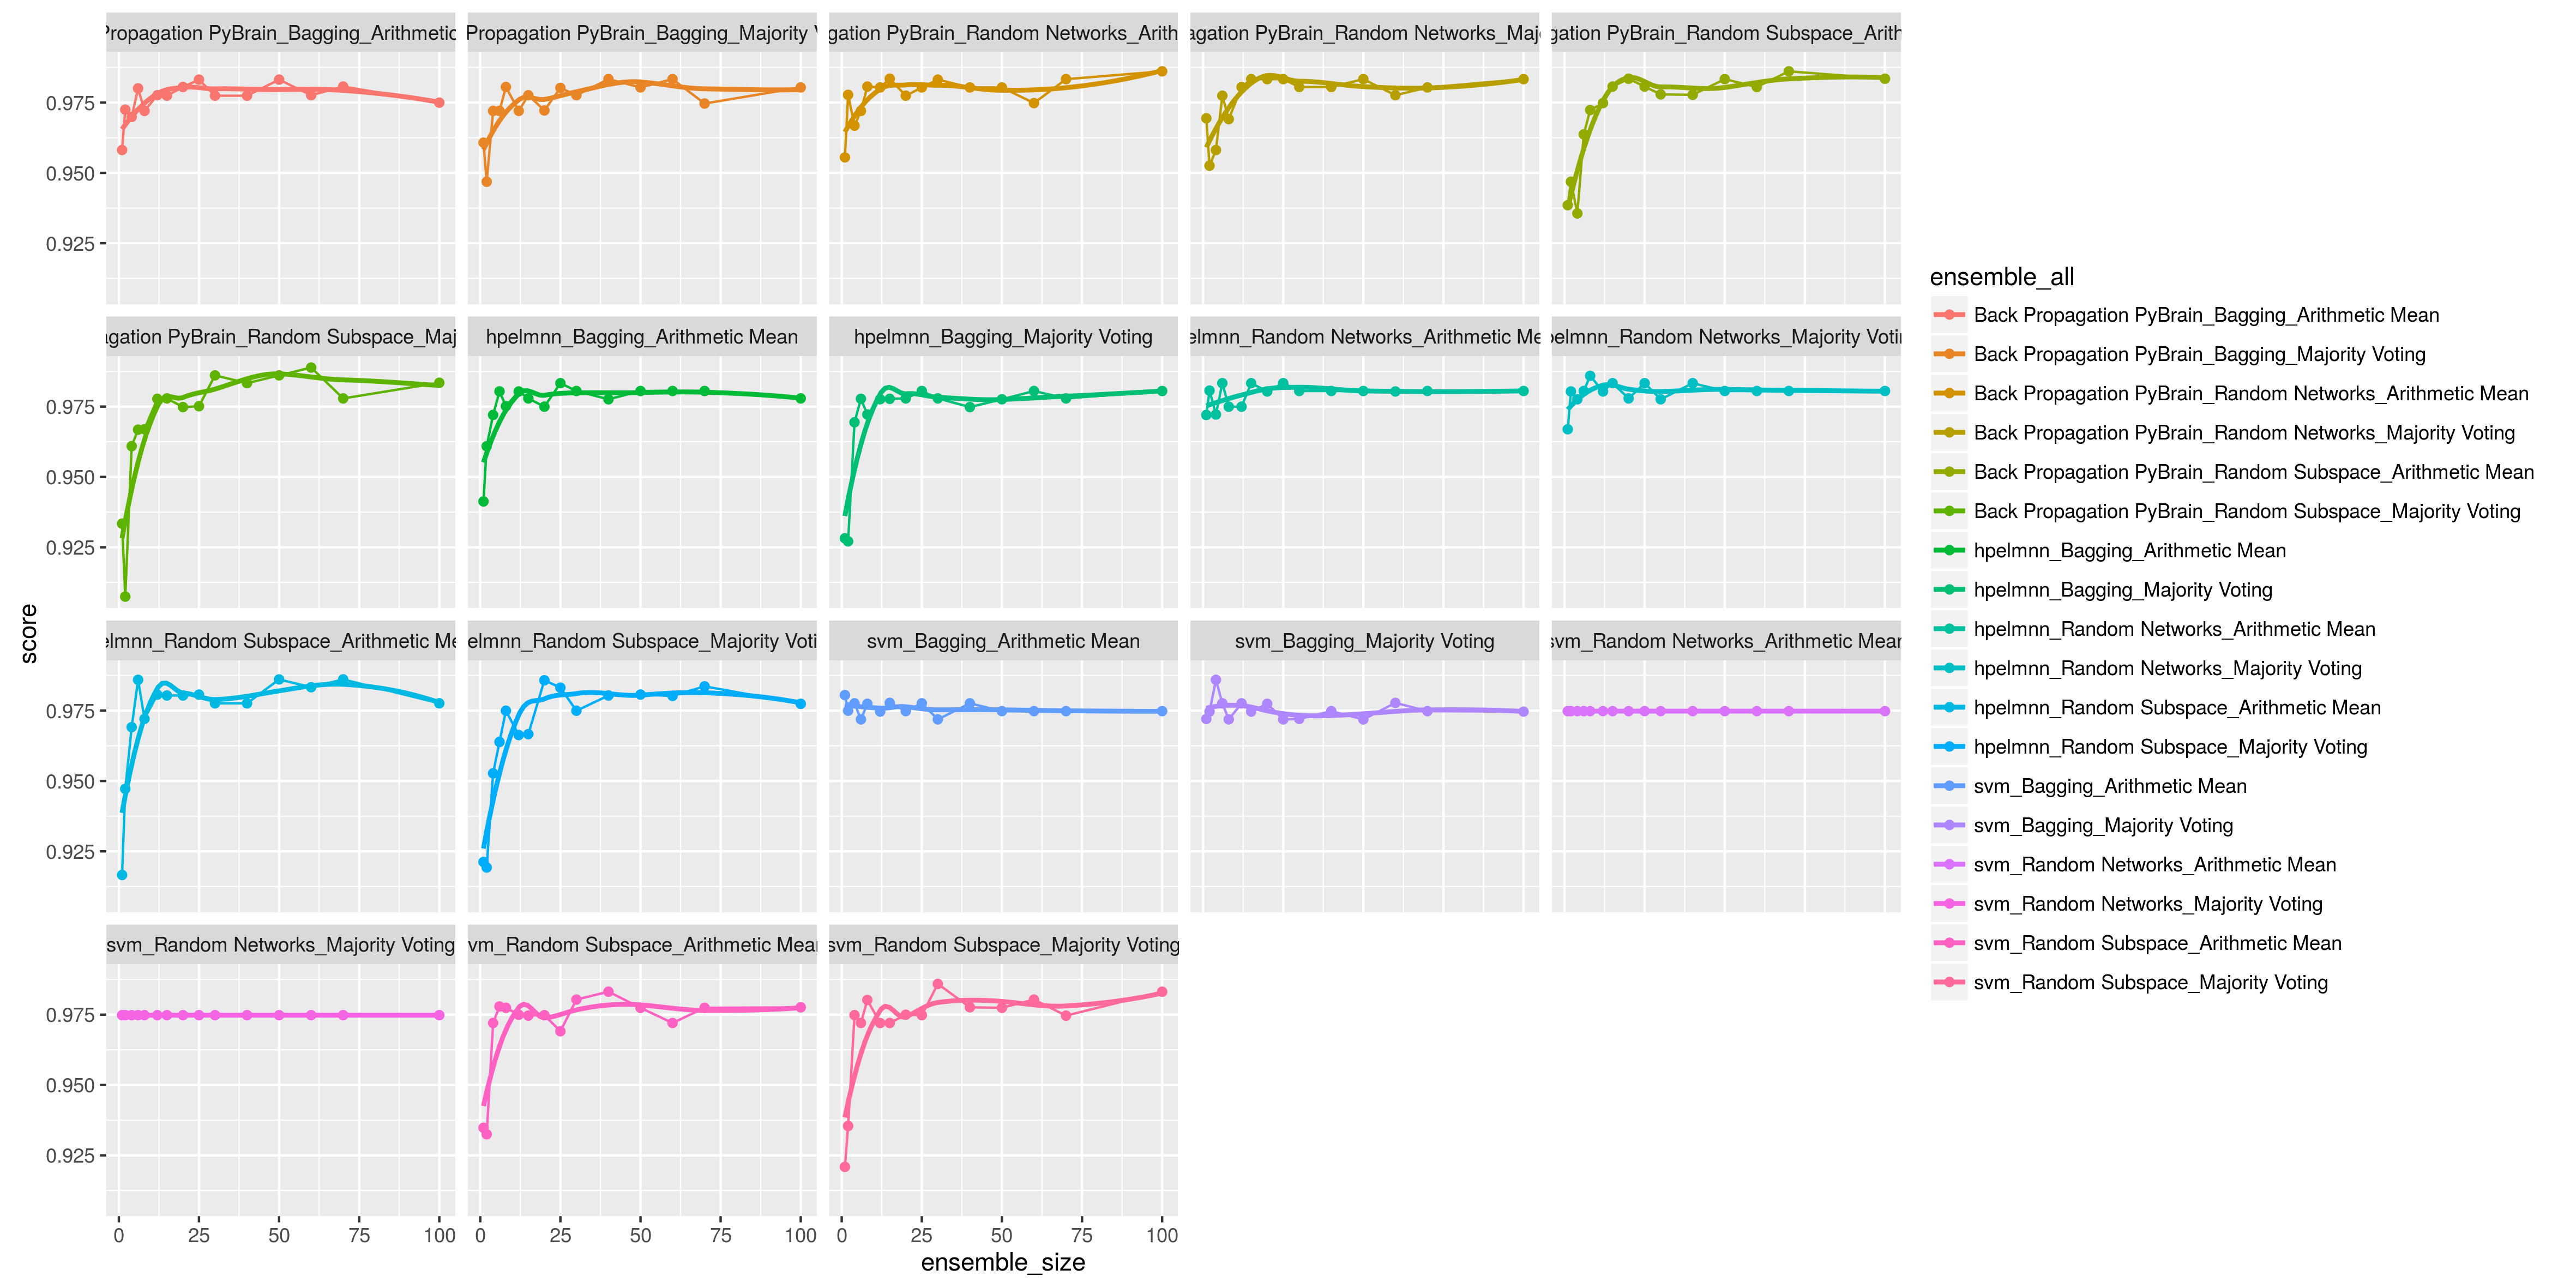
\includegraphics[width=1.0\textwidth]{type2_score_size_model_dermatology}
    \centering
    \caption{Wyniki skuteczności wszystkich typów komitetów na zbiorze \textit{dermatology}}
    \label{fig:type2_dermatology}
\end{figure}

Na wynikach badań przeprowadzonych na częsci zestawów danych zwiększenie liczby członków komitetu powyżej dwudziestu skutkowało ustabilizowaniem otrzymywanych skuteczności. Zjawisko to przedstawia wykres \ref{fig:type2_breast_cancer}.

\begin{figure}[H]
	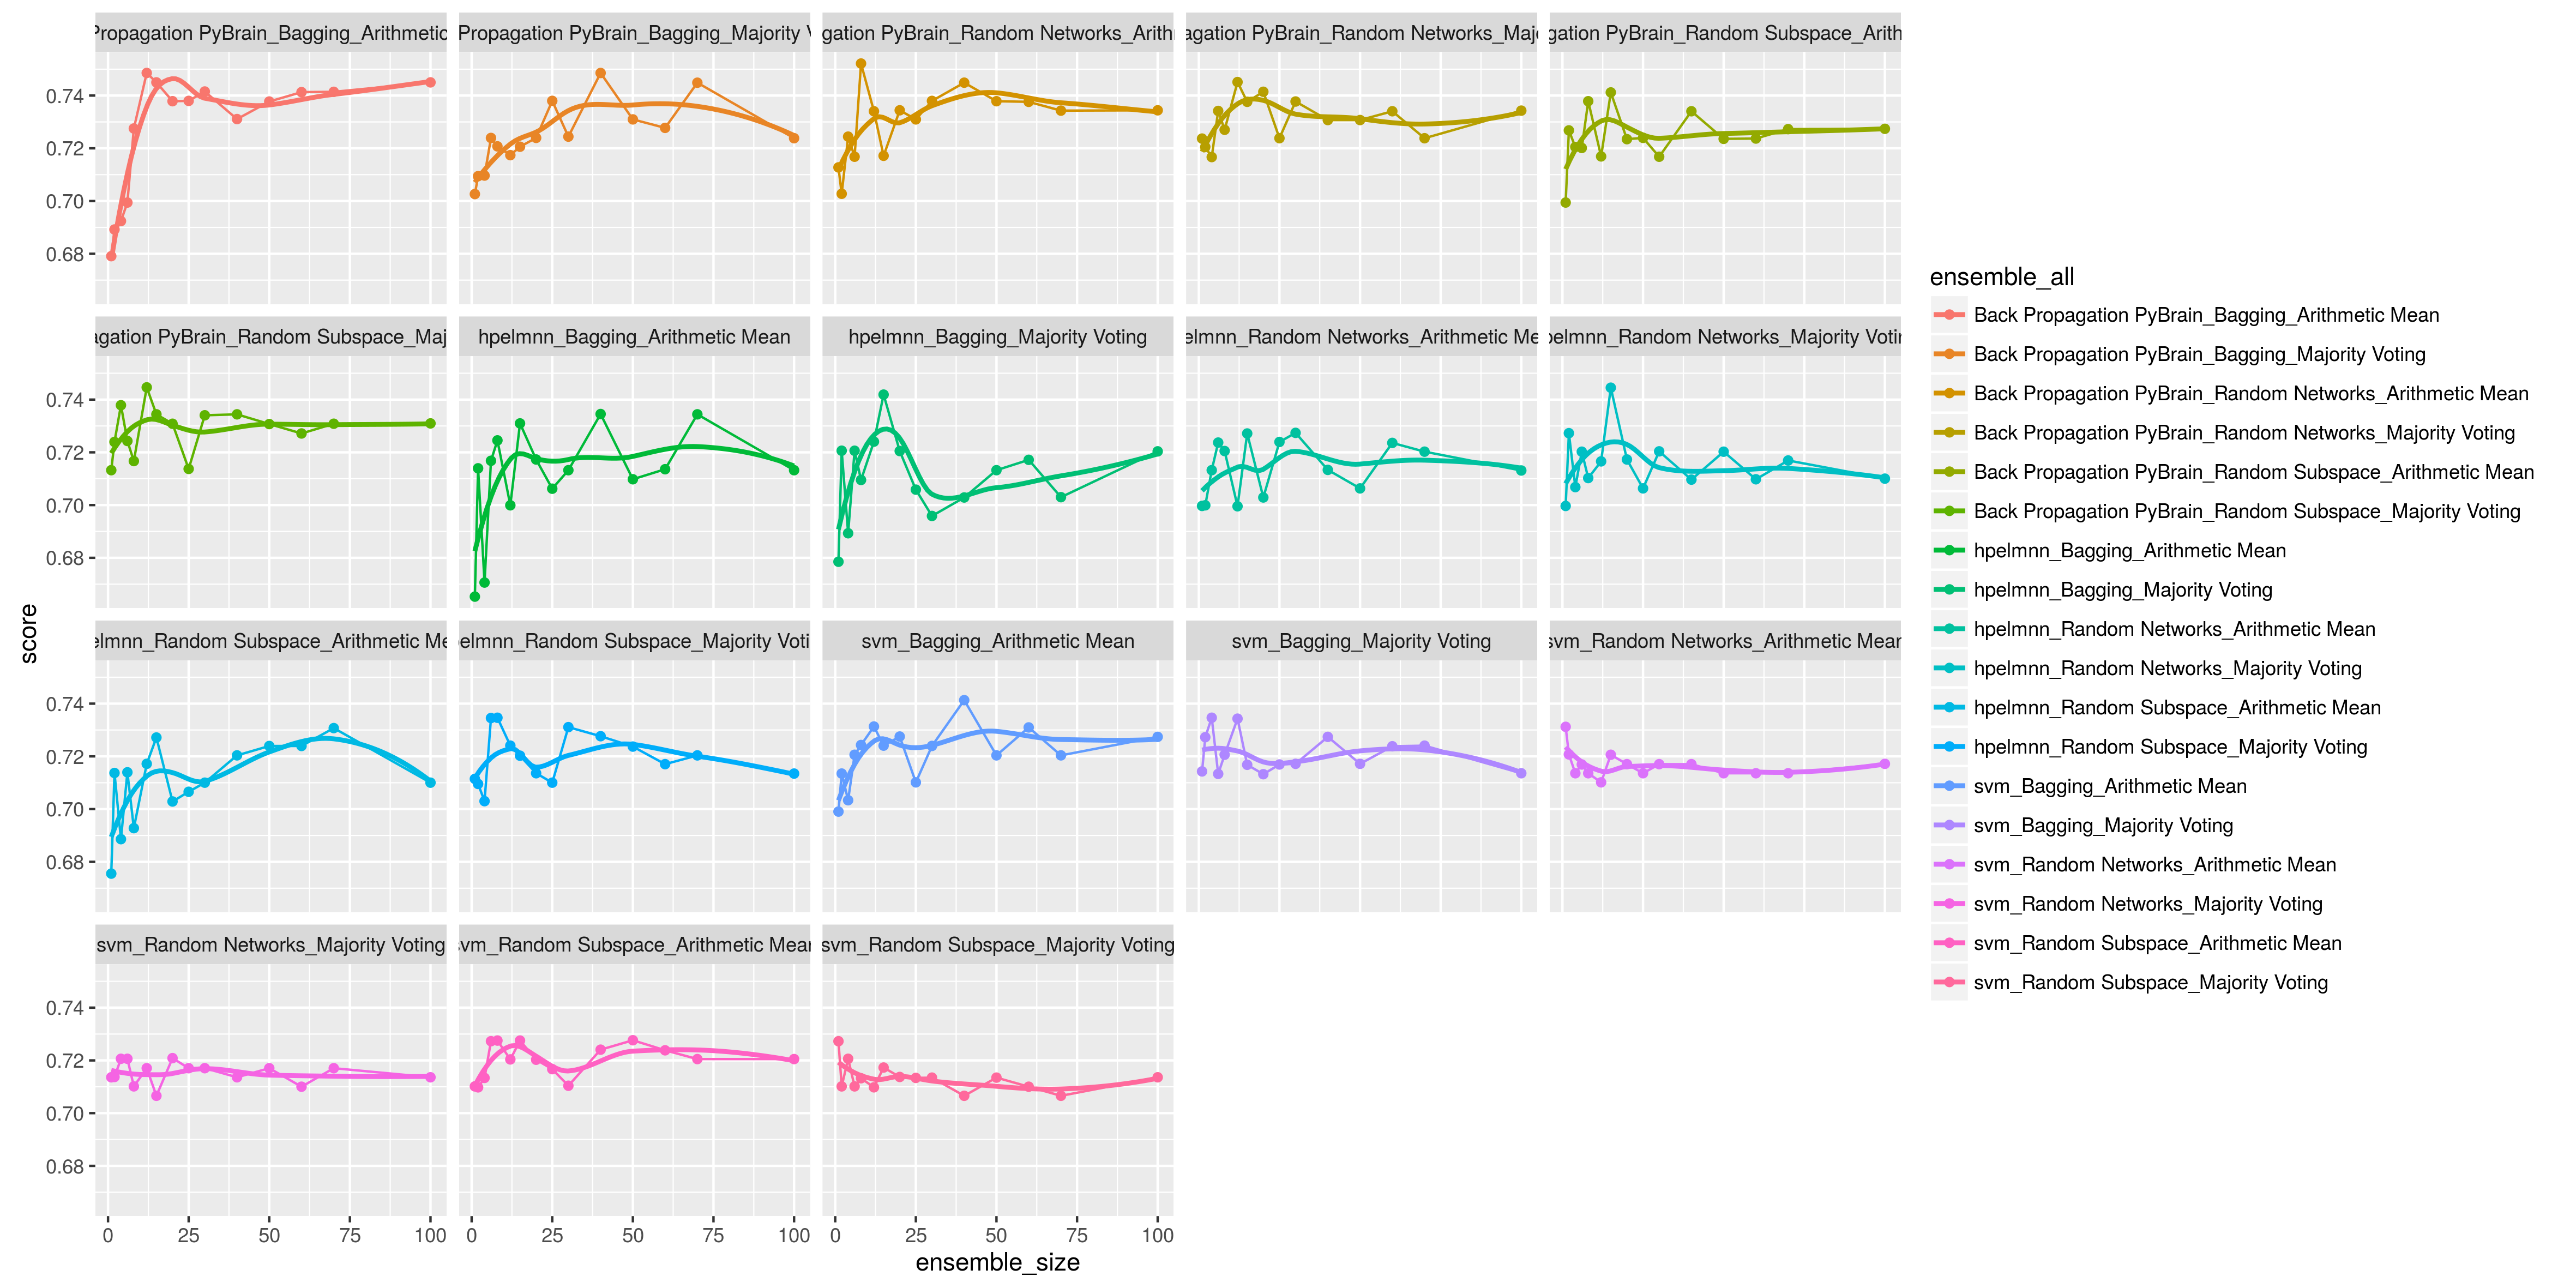
\includegraphics[width=1.0\textwidth]{type2_score_size_model_breast_cancer}
    \centering
    \caption{Wyniki skuteczności wszystkich typów komitetów na zbiorze \textit{breast\_cancer}}
    \label{fig:type2_breast_cancer}
\end{figure}

\section{Skuteczność komitetów w zależności od zastosowanego modułu decyzyjnego}

Na rysunku \ref{fig:aggr_rank_voting} przedstawiono ranking komitetów według typów głosowania. Jak widać \textit{Arithmetic Mean} uzyskał nieco lepszy wynik. Prawdopodobnie jest to związane z tym, że metoda ta bierze pod uwagę pełną informacje o cząstkowych decyzjach podejmowanych przez klasyfikatory bazowe, w tym wypadku są to wektory wsparć dla poszczególnych klas.

\begin{figure}[H]
	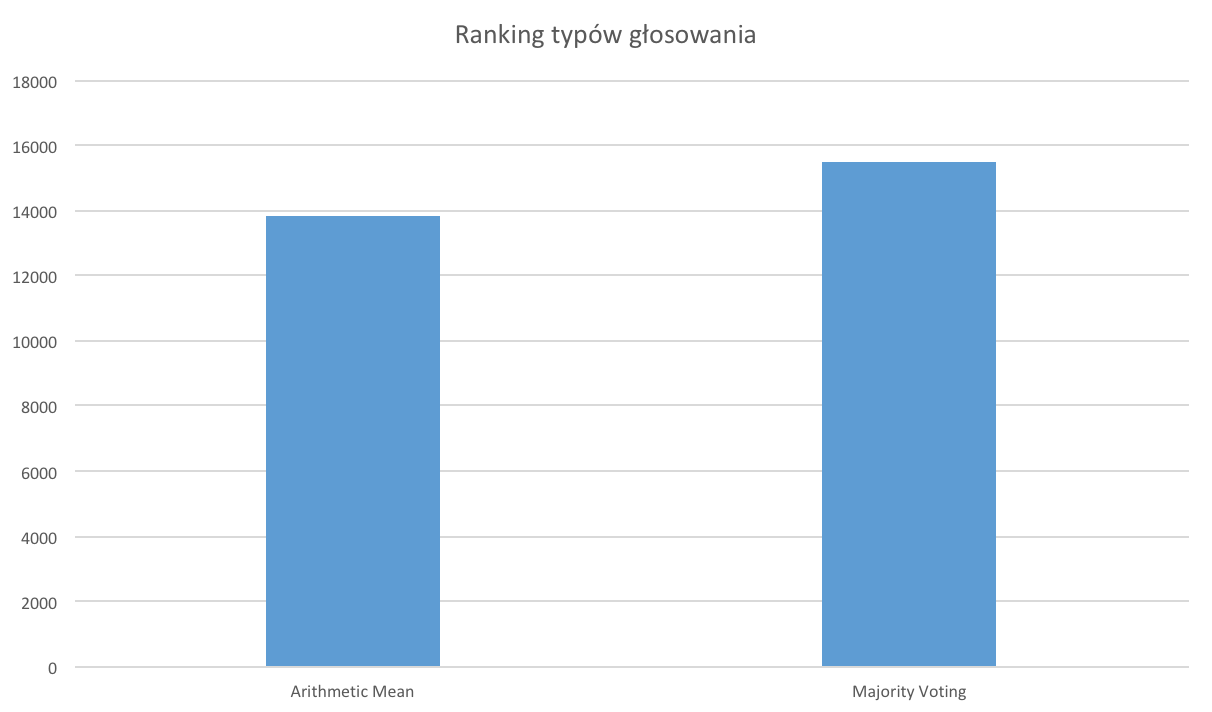
\includegraphics[width=0.5\textwidth]{aggregated_rank_voting}
    \centering
    \caption{Zagregowany ranking systemów głosowania}
    \label{fig:aggr_rank_voting}
\end{figure}

\section{Wyniki badanych modeli zagregowane ze wszystkich zestawów danych}
Otrzymane w badaniach wyniki ukazują, który model klasyfikujący najlepiej radzi sobie z opisanym przez określony zbiór danych problemem. Jednak aby uzyskać ranking modeli w ogólnym przypadku należy pośrednie wyniki ze wszystkich zbiorów danych zagregować. Użyto do tego metody polegającej na przypisaniu każdemu modelowi rang oznaczających jego skuteczność względem innych modeli w każdym problemie osobno. Im mniejsza jest wartość rangi, tym model miał wyższą skuteczność dla danego zbioru obiektów. Następnie zsumowano wszystkie rangi każdego modelu. Model z najniższą sumą traktowany jest jako najlepszy. Powyższą procedurę powtórzono dla wszystkich zbadanych rozmiarów komitetów. Otrzymano więc zależność ogólnego wyniku modelu od rozmiaru komitetu. Wykres tych zależności przedstawia rysunek \ref{fig:aggr_rank}.

\begin{figure}[H]
	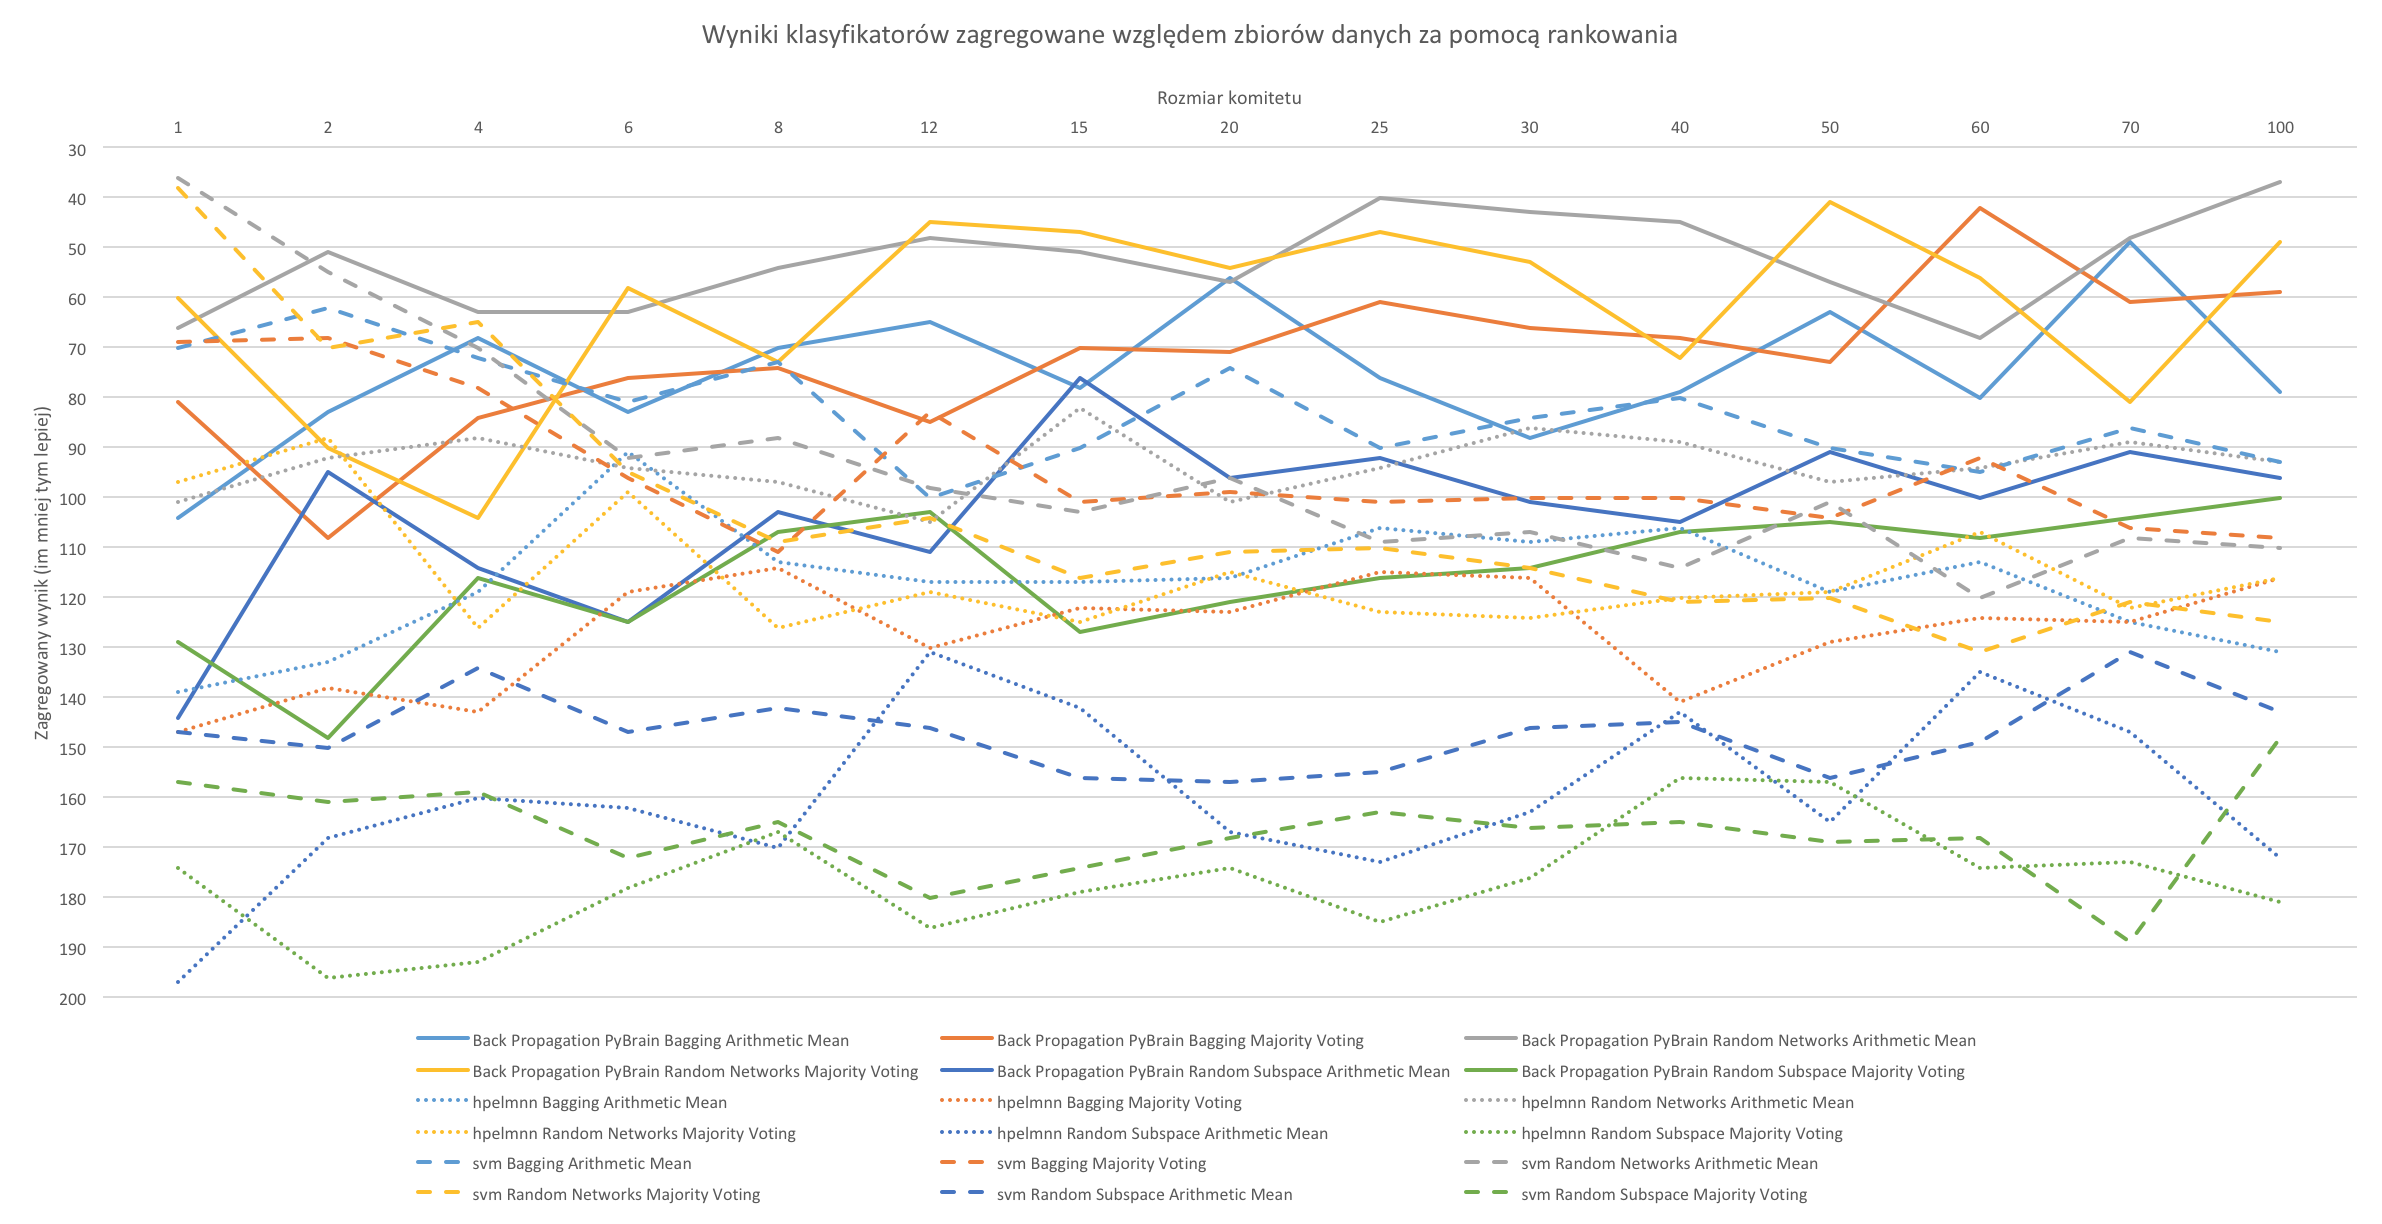
\includegraphics[width=1.0\textwidth]{aggregated_rank}
    \centering
    \caption{Zagregowany ranking badanych modeli klasyfikujących}
    \label{fig:aggr_rank}
\end{figure}


\chapter{Podsumowanie}
Analiza otrzymanych wyników pozwoliła na wysunięcie kilku wniosków dotyczących badań przeprowadzonych podczas realizacji projektu.

Ważnym aspektem badania skuteczności modeli jest wcześniejsze przygotowanie danych. Należy dobierać zróżnicowane zbiory tak, aby otrzymać jak najszerszy obraz skuteczności każdego z modelu. Istotne jest również przetworzenie danych, ponieważ implementacje sieci neuronowych zwykle oczekują sygnałów wejściowych w postaci liczb rzeczywistych z zakresu $\{0, 1\}$. Podczas realizacji projektu przygotowano narzędzia ułatwiające przystosowanie nowych zbiorów danych do istniejącego systemu.

W przypadku badania różnych typów klasyfikatorów nie jest kluczowe uzyskanie jak najlepszej skuteczności pojedynczego klasyfikatora, natomiast ważny jest krótki czas potrzebny na naukę sieci, z uwagi na duże rozmiary komitetów w badaniach. Znalezienie dobrego stosunku skuteczności pojedynczego klasyfikatora bazowego do czasu potrzebnego na  przeprowadzanie dla niego pełnych badań może być trudnym zadaniem.

Jednym z celów projektu było wyznaczenie zależności skuteczności komitetu od jego rozmiaru. Wybranie odpowiednich wartości okazało się istotne z punktu widzenia czasu przeprowadzania badań. Różnice w skuteczności pomiędzy dużymi wartościami rozmiaru dla danego modelu są mniejsze niż dla małych rozmiarów, dlatego warto zmniejszać zagęszczenie próbek rozmiaru wraz z jego wzrostem. Pozwala to zmniejszyć czas badań przy zachowaniu ogólnej zależności skuteczności od rozmiaru.

\appendix
\chapter{Graficzna reprezentacja wyników}

\begin{figure}[H]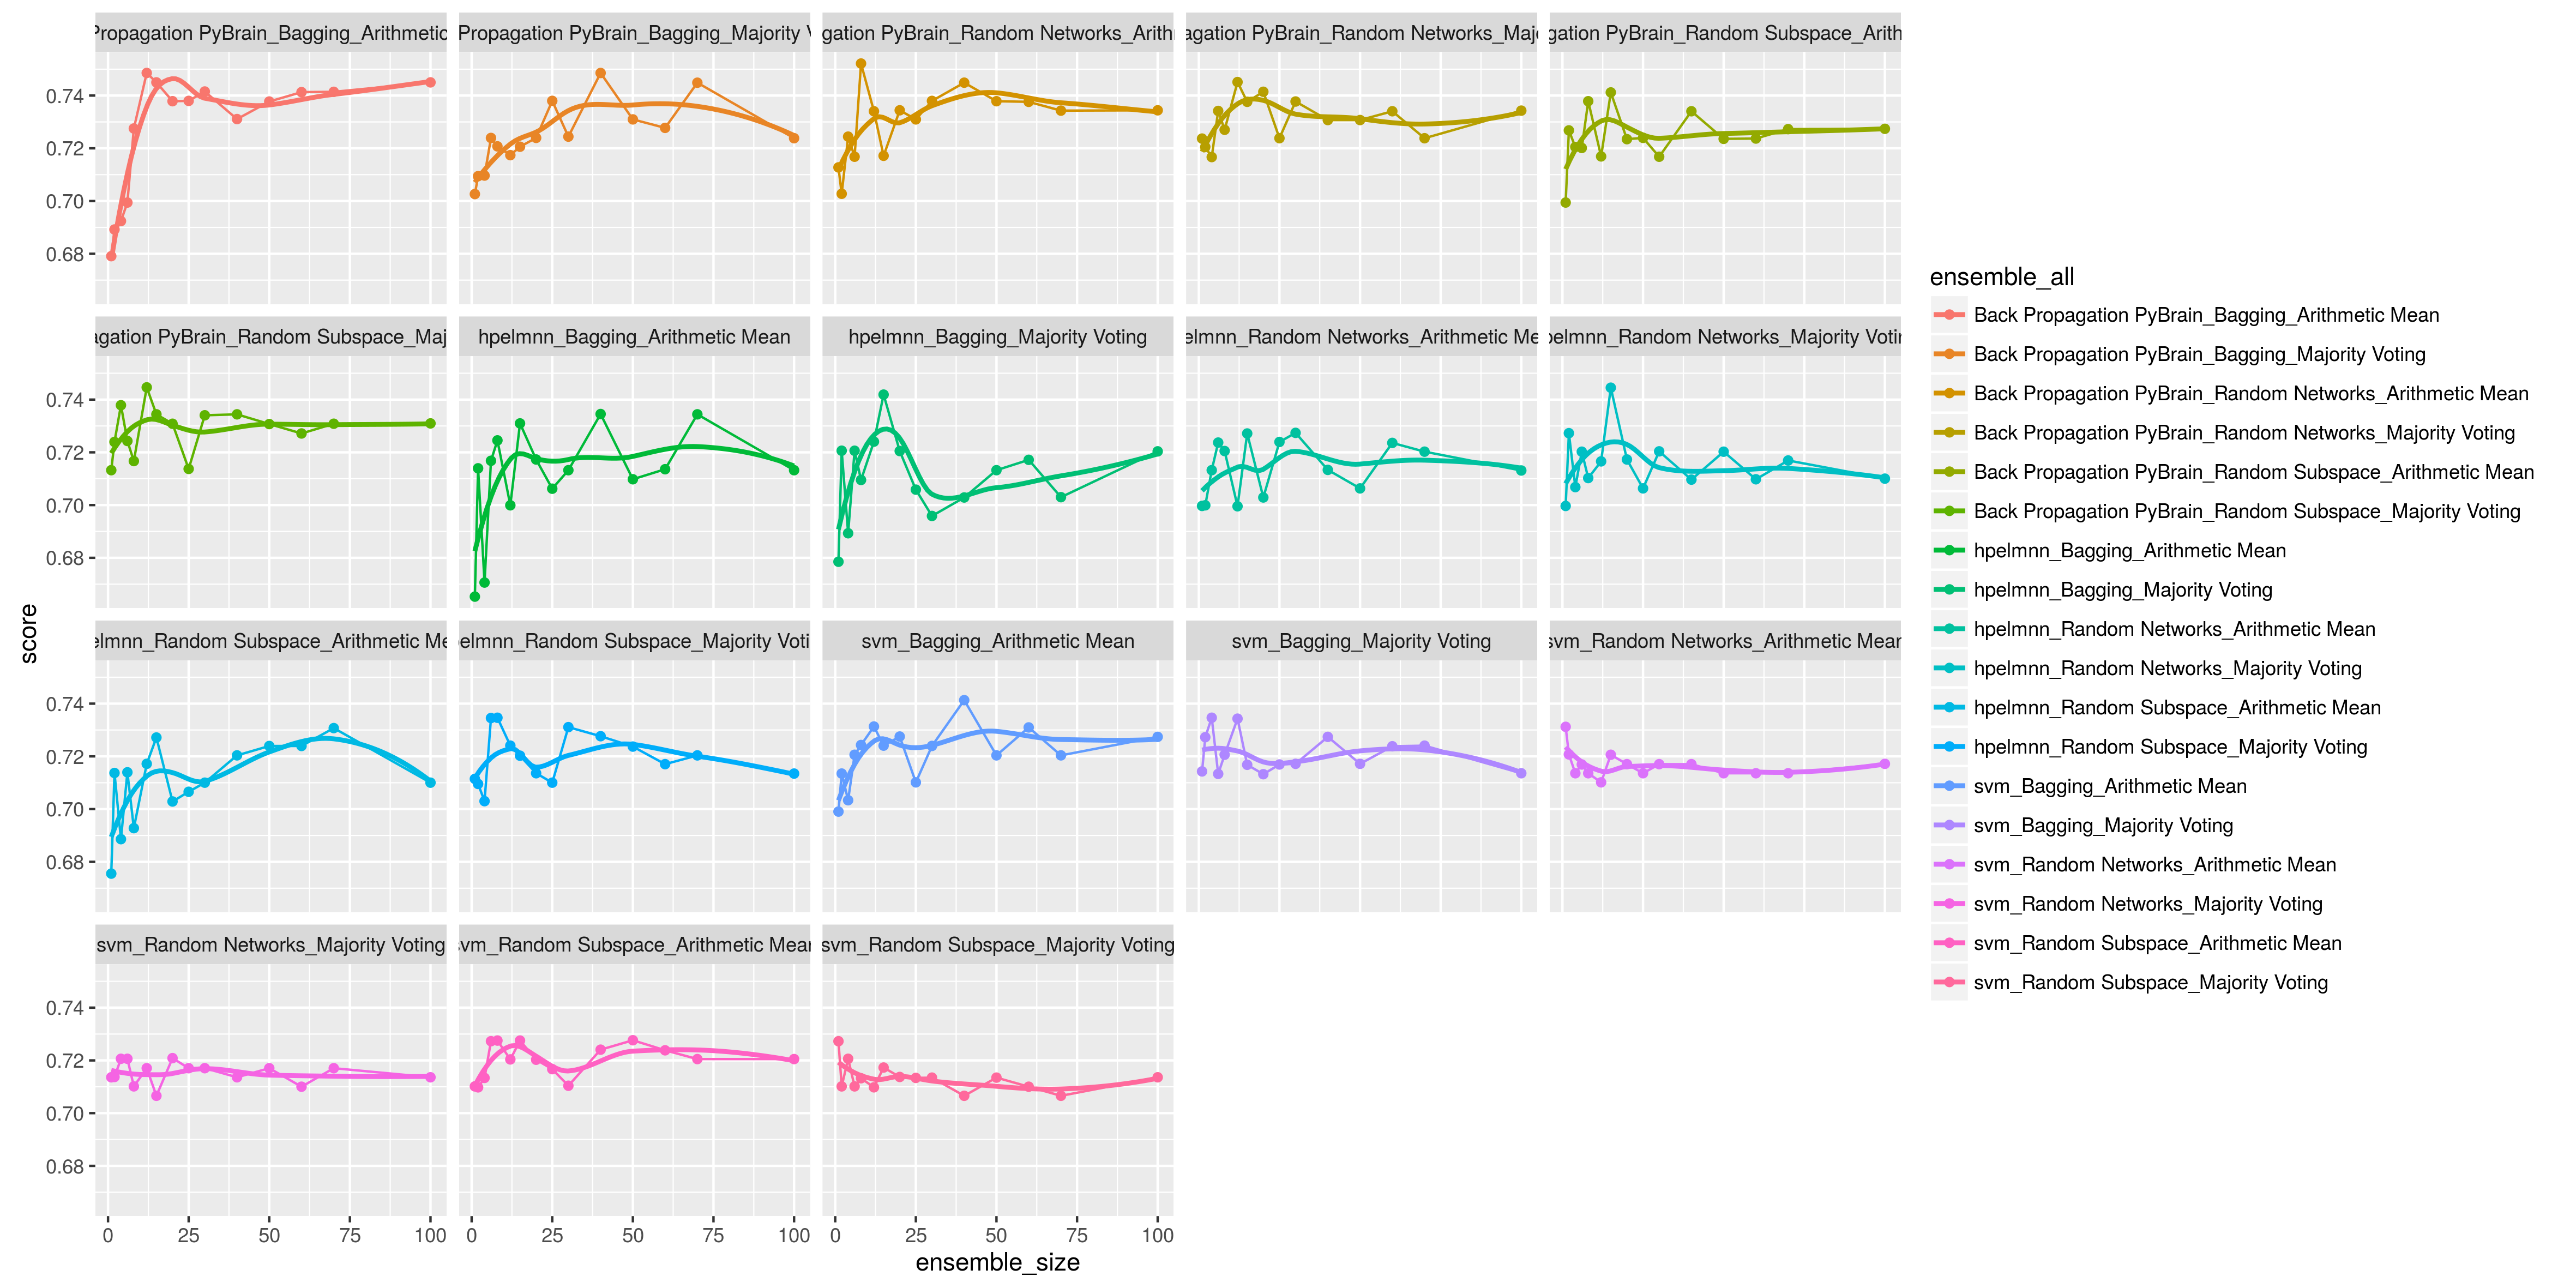
\includegraphics[width=1.0\textwidth]{type2_score_size_model_breast_cancer}\centering\caption{breast\_cancer}\end{figure}
\begin{figure}[H]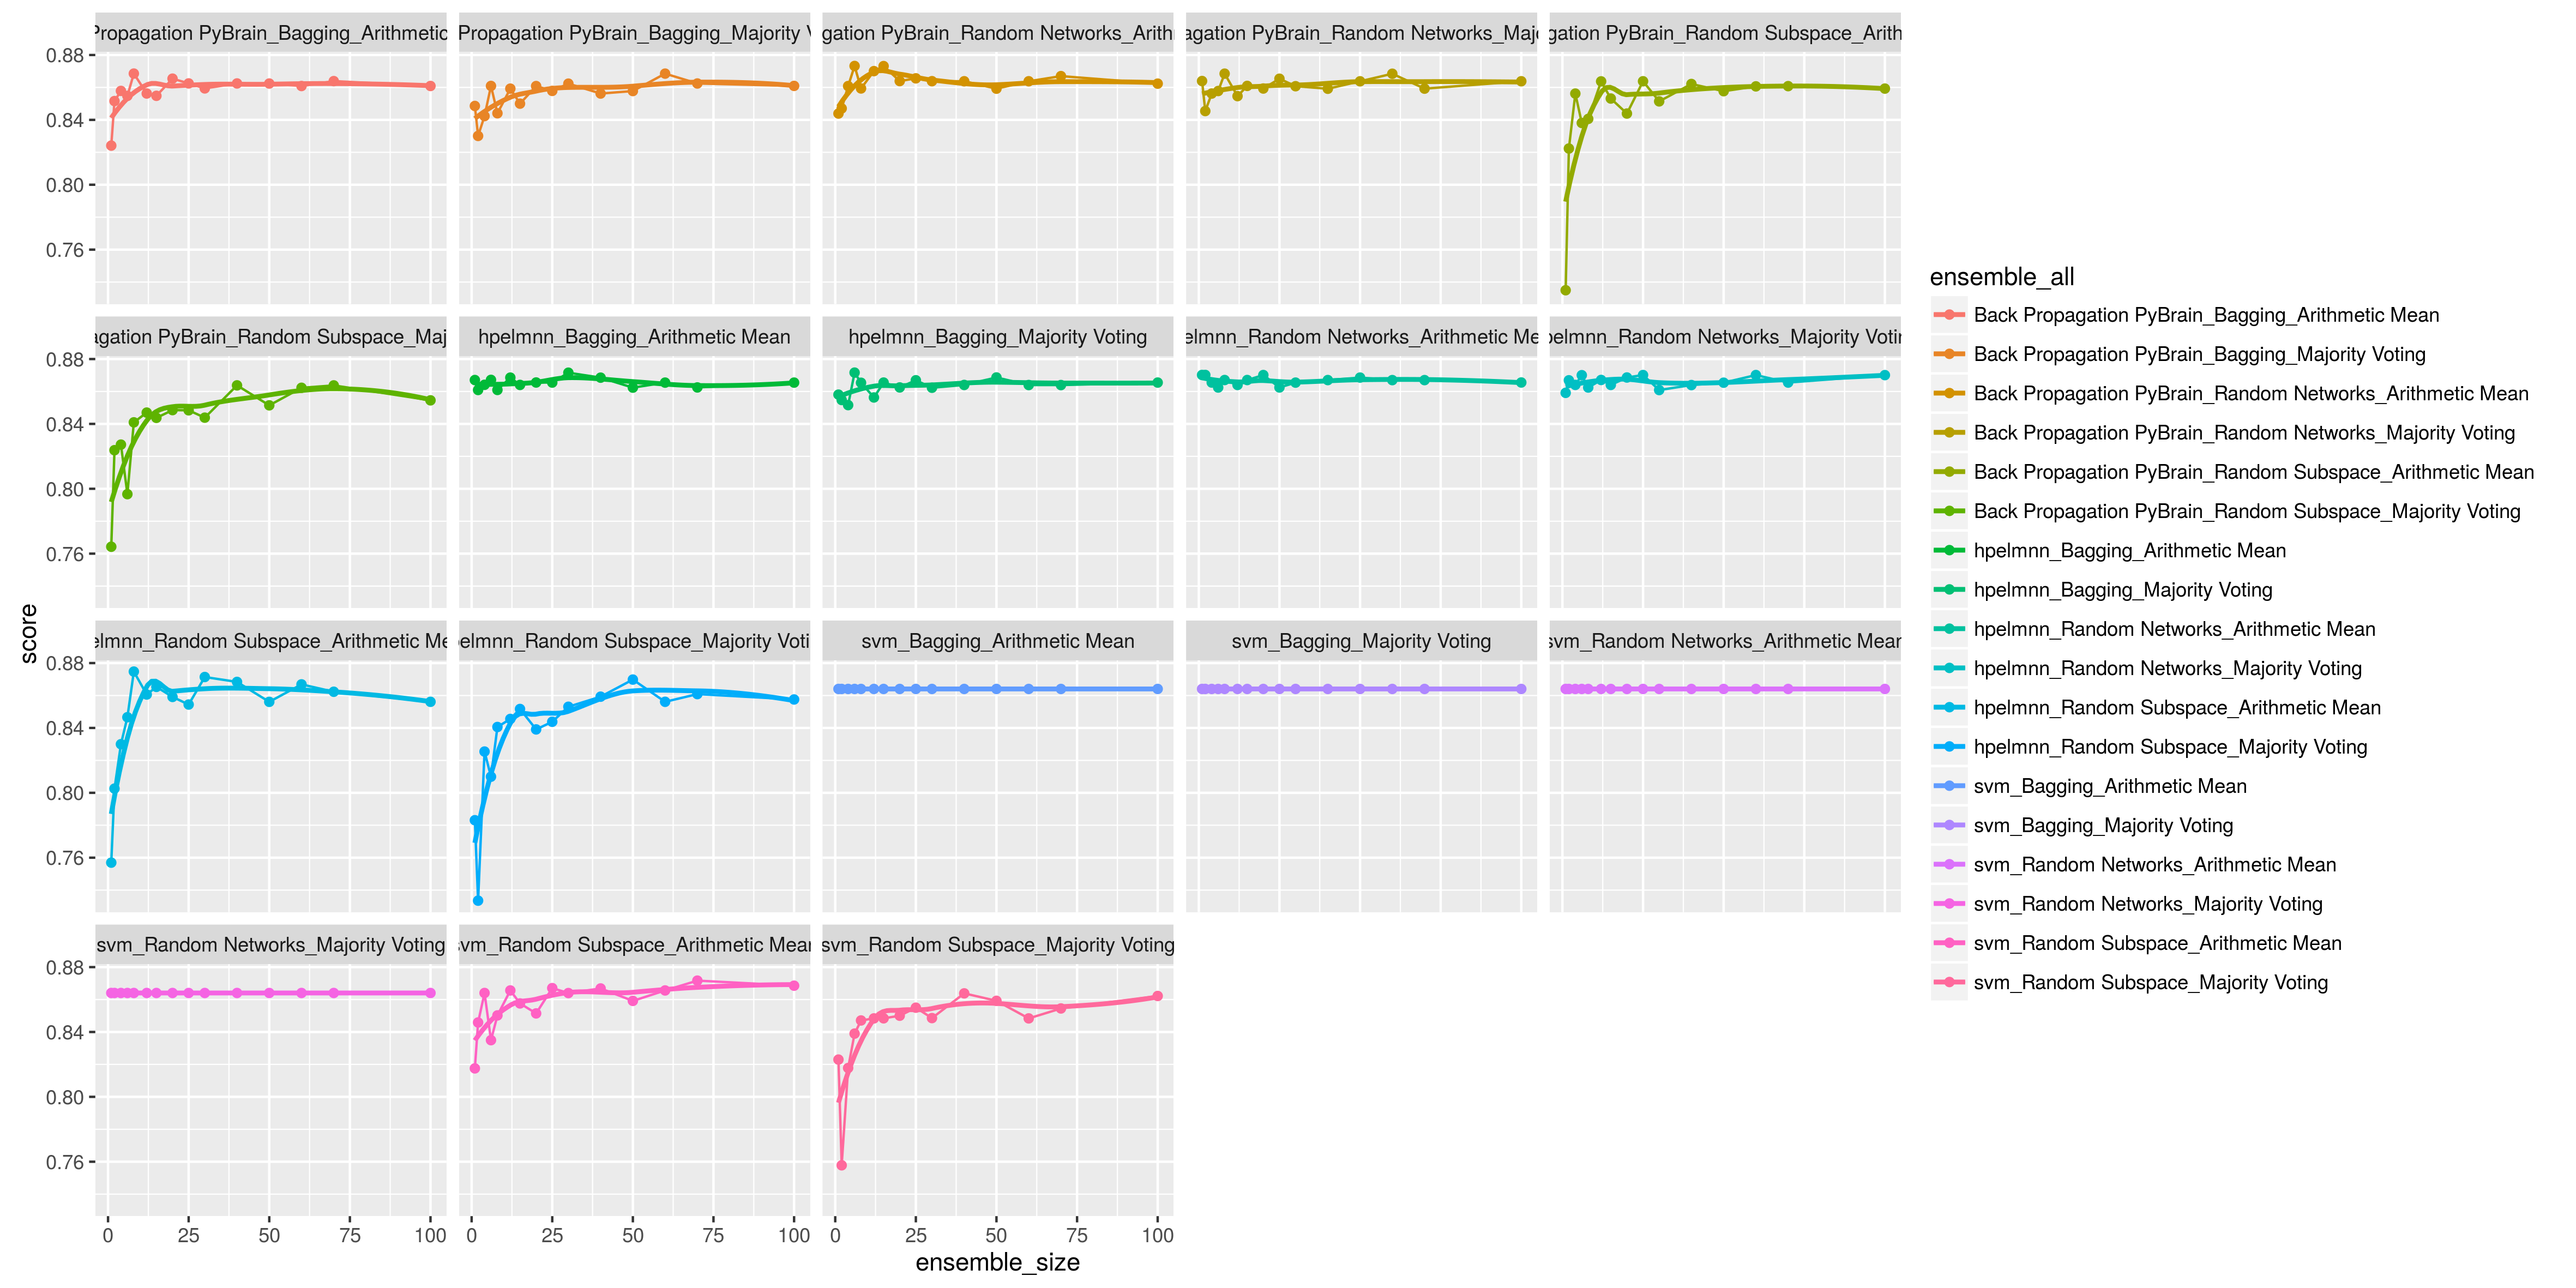
\includegraphics[width=1.0\textwidth]{type2_score_size_model_crx}\centering\caption{crx}\end{figure}
\begin{figure}[H]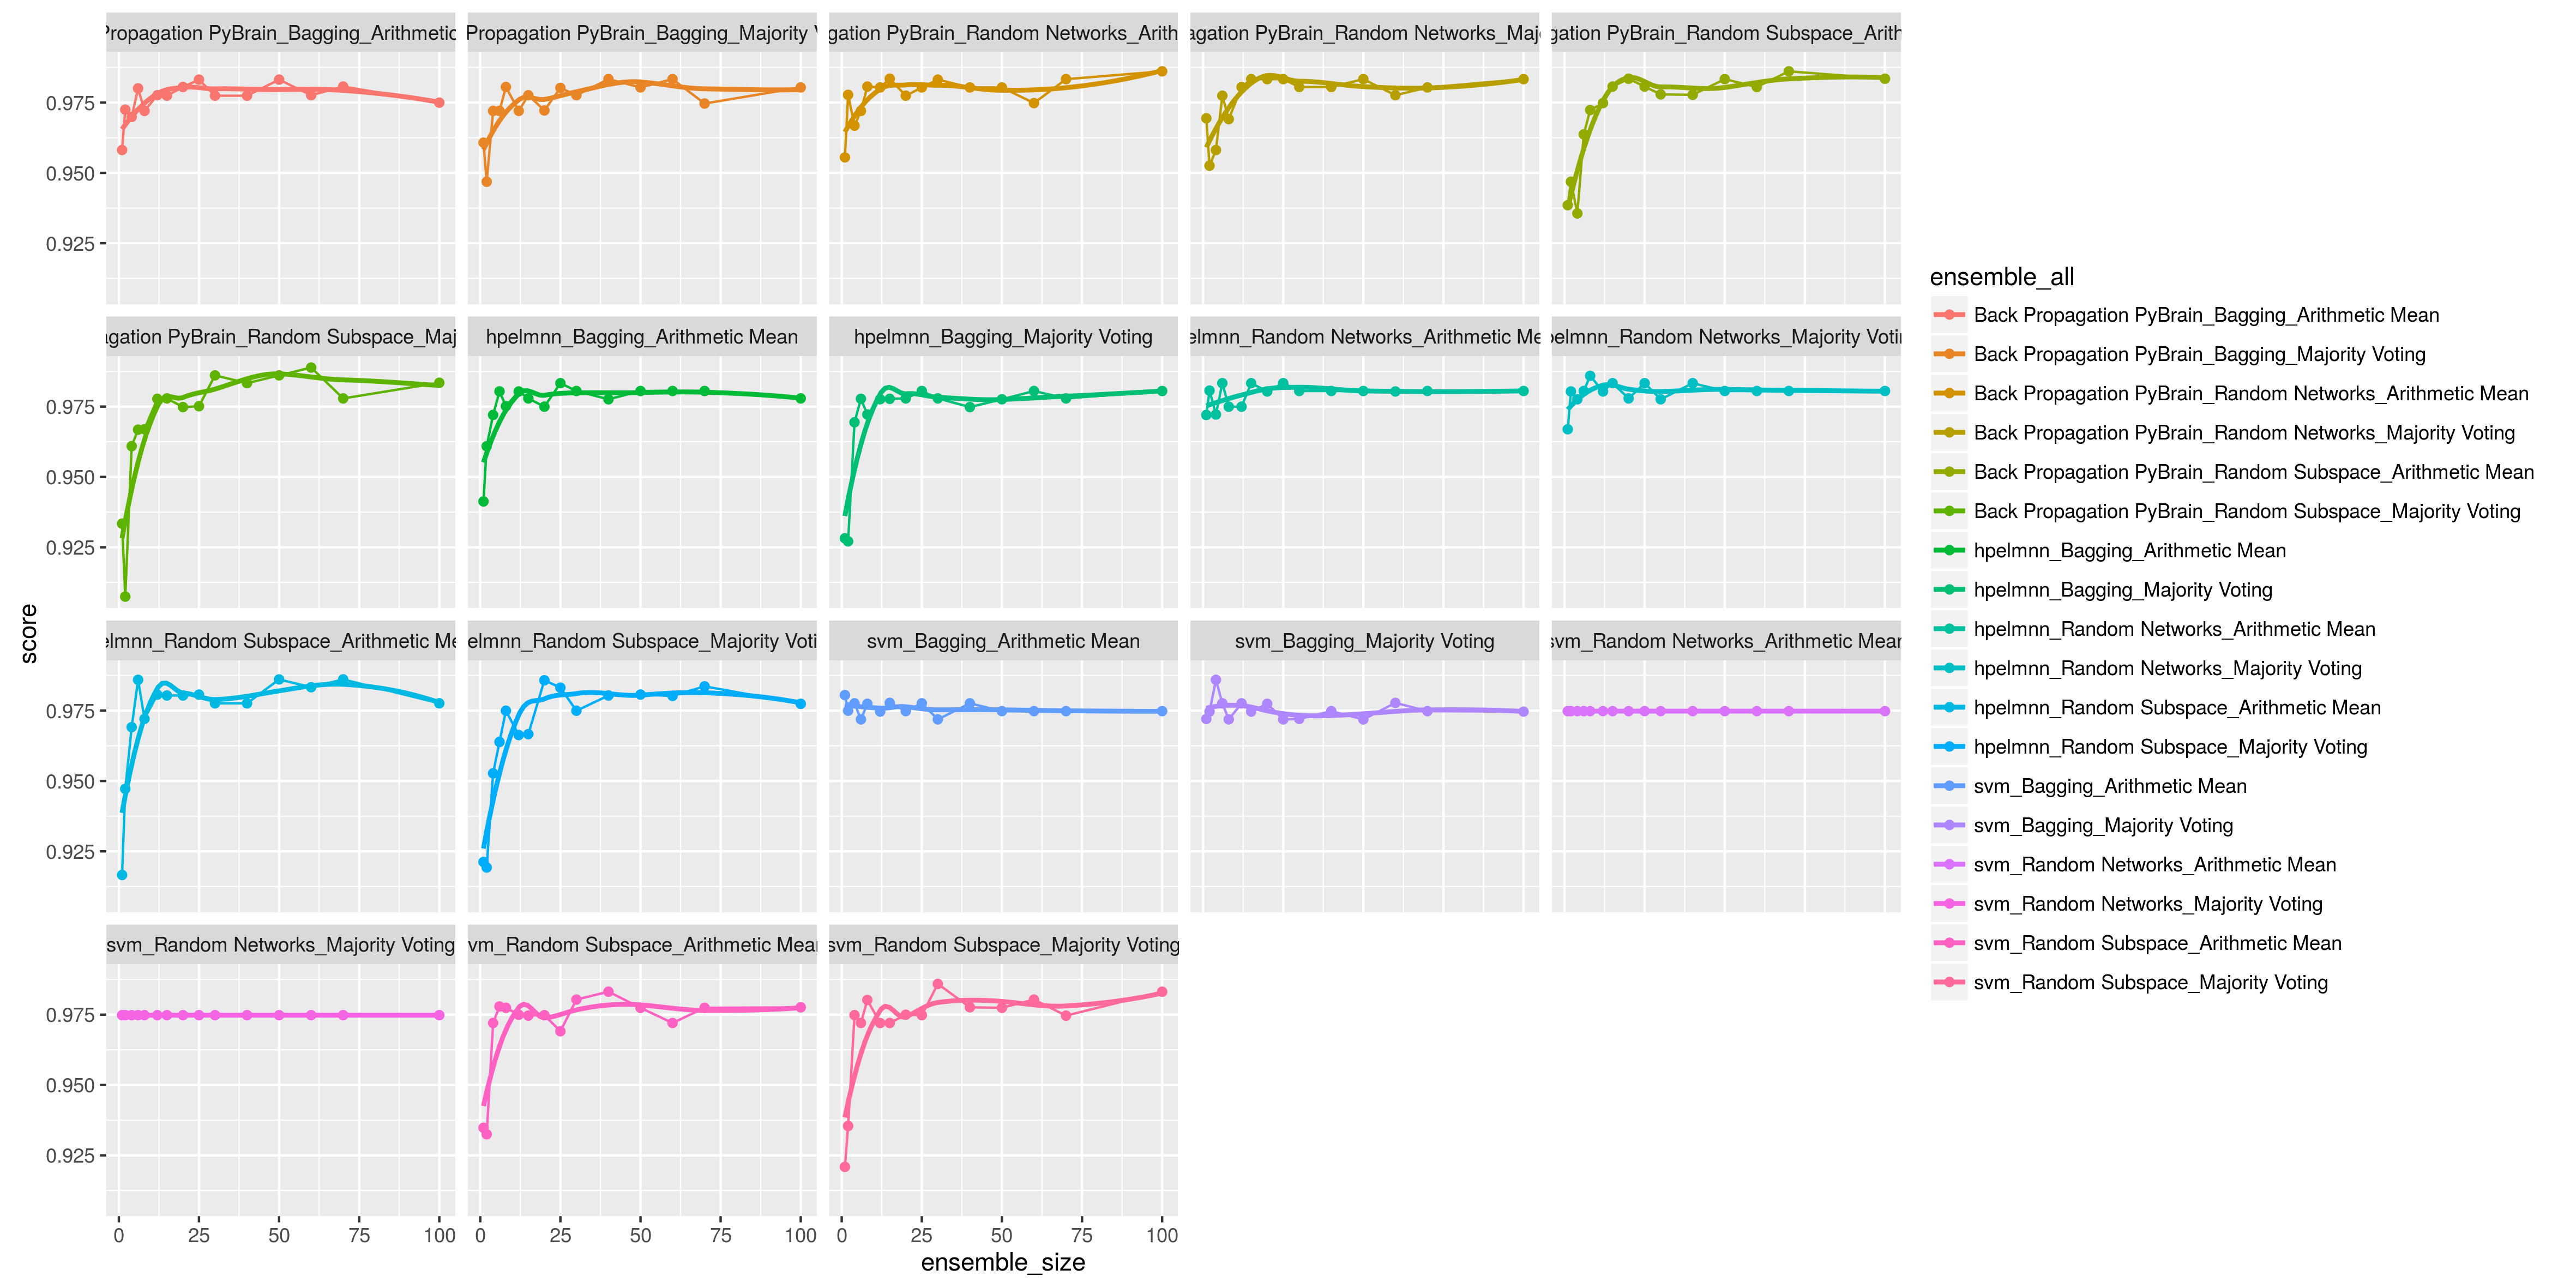
\includegraphics[width=1.0\textwidth]{type2_score_size_model_dermatology}\centering\caption{dermatology}\end{figure}
\begin{figure}[H]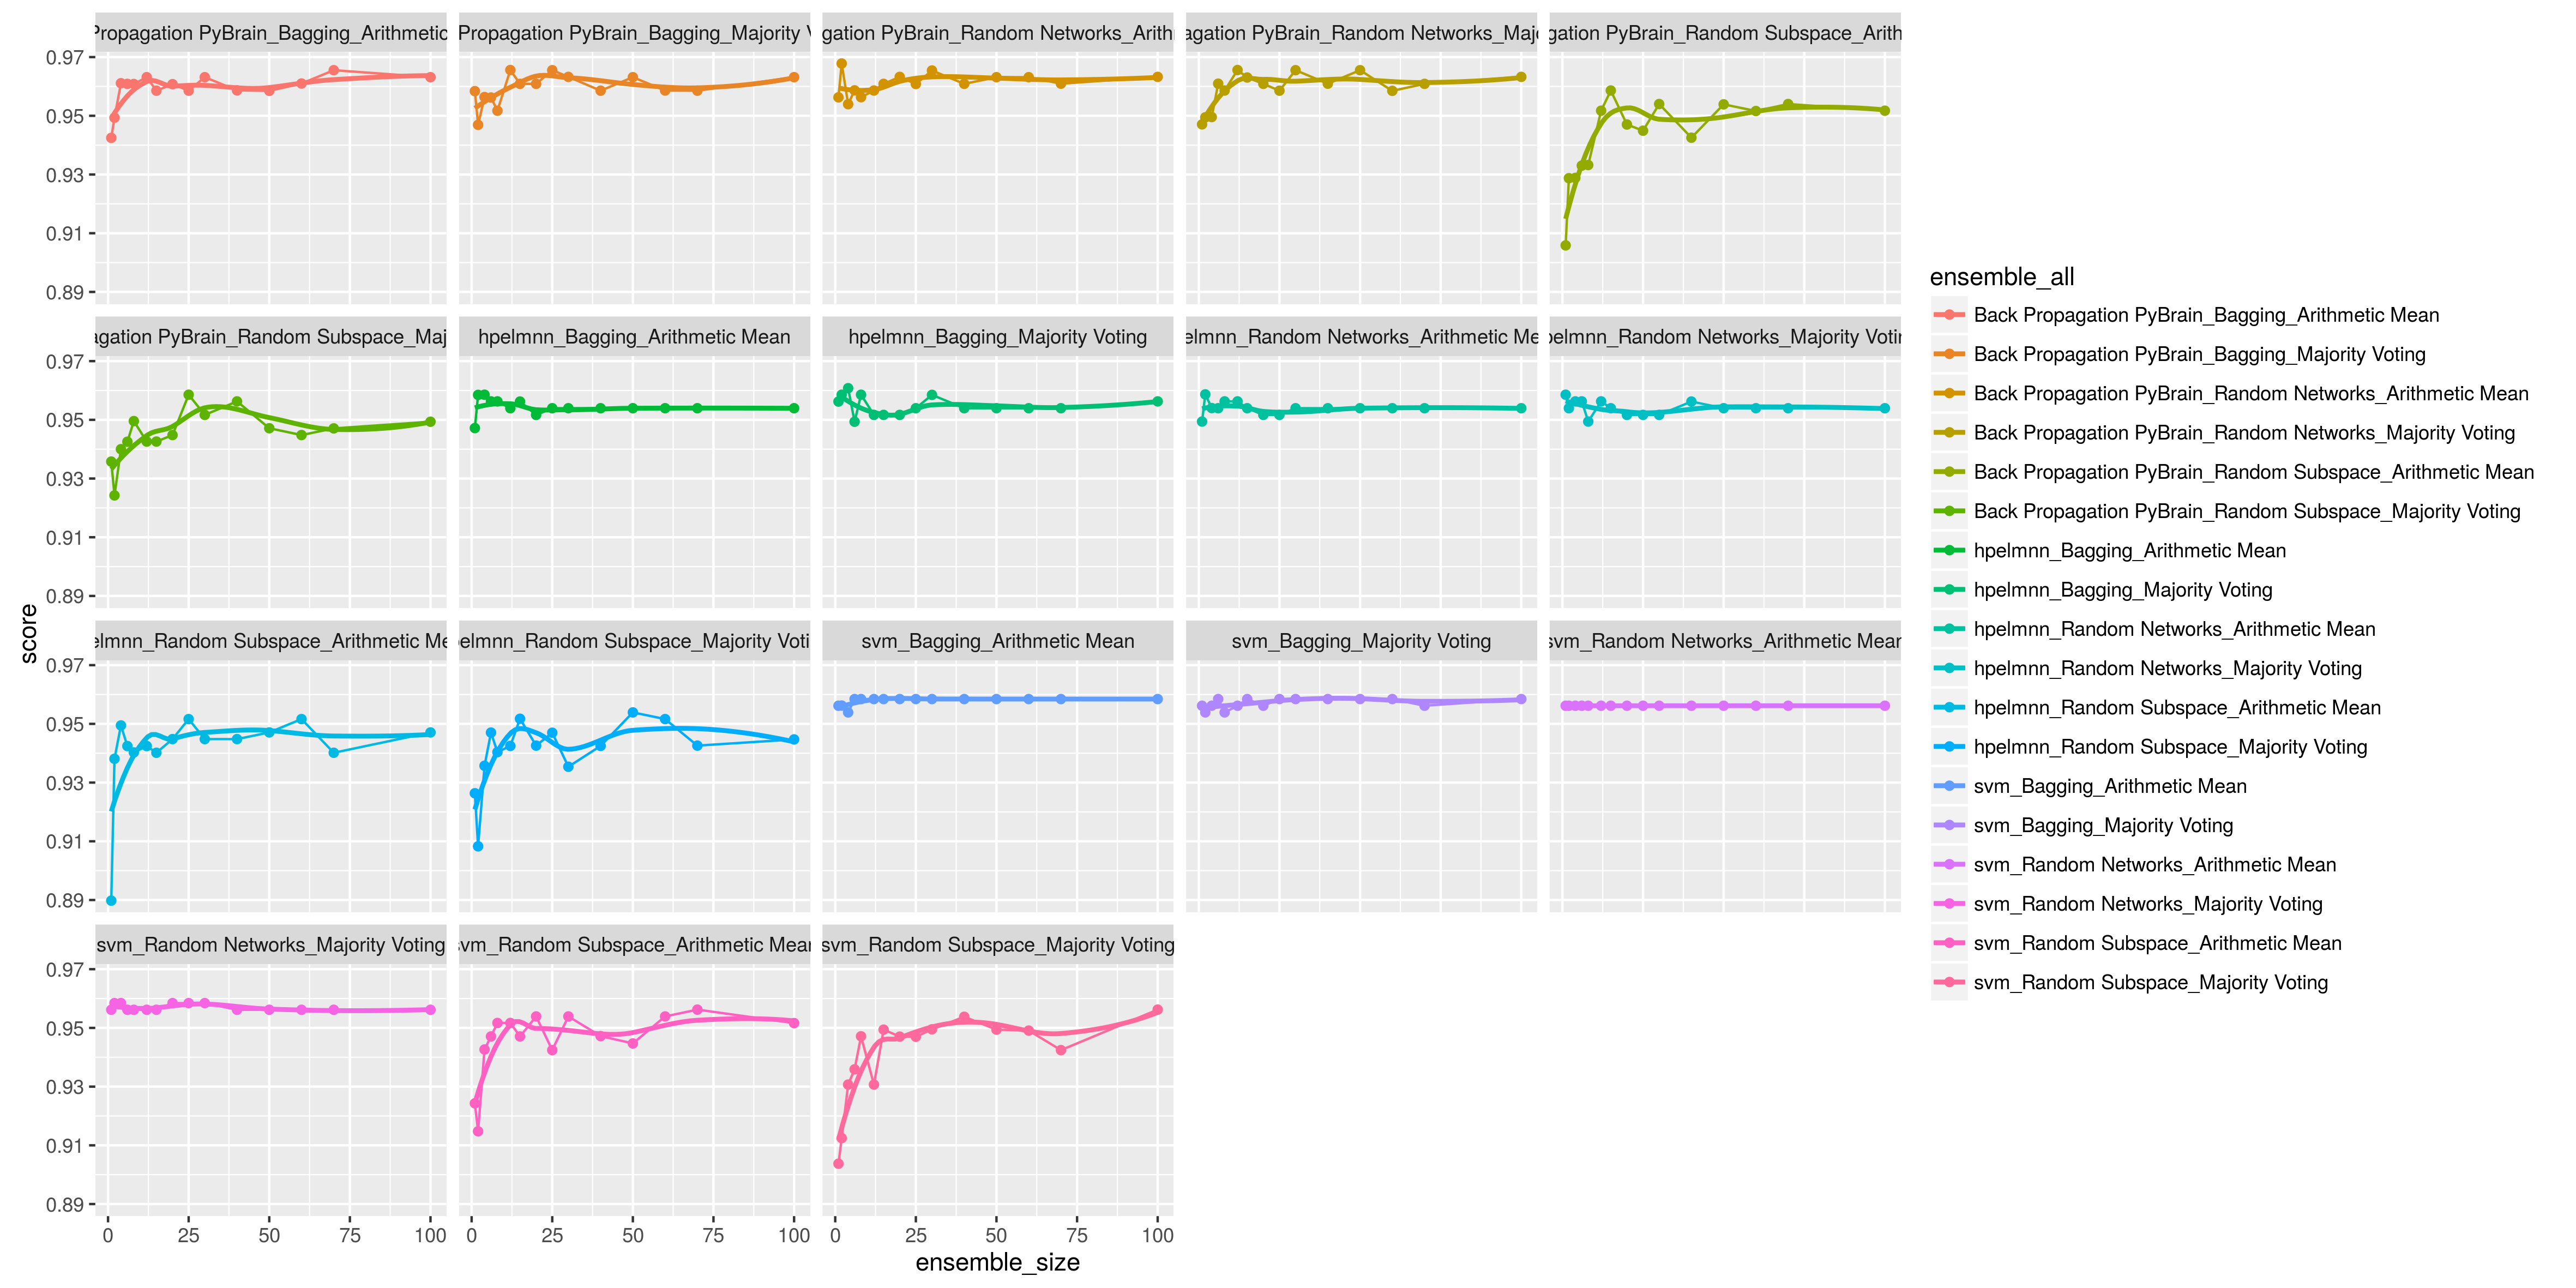
\includegraphics[width=1.0\textwidth]{type2_score_size_model_house_votes}\centering\caption{house\_votes}\end{figure}
\begin{figure}[H]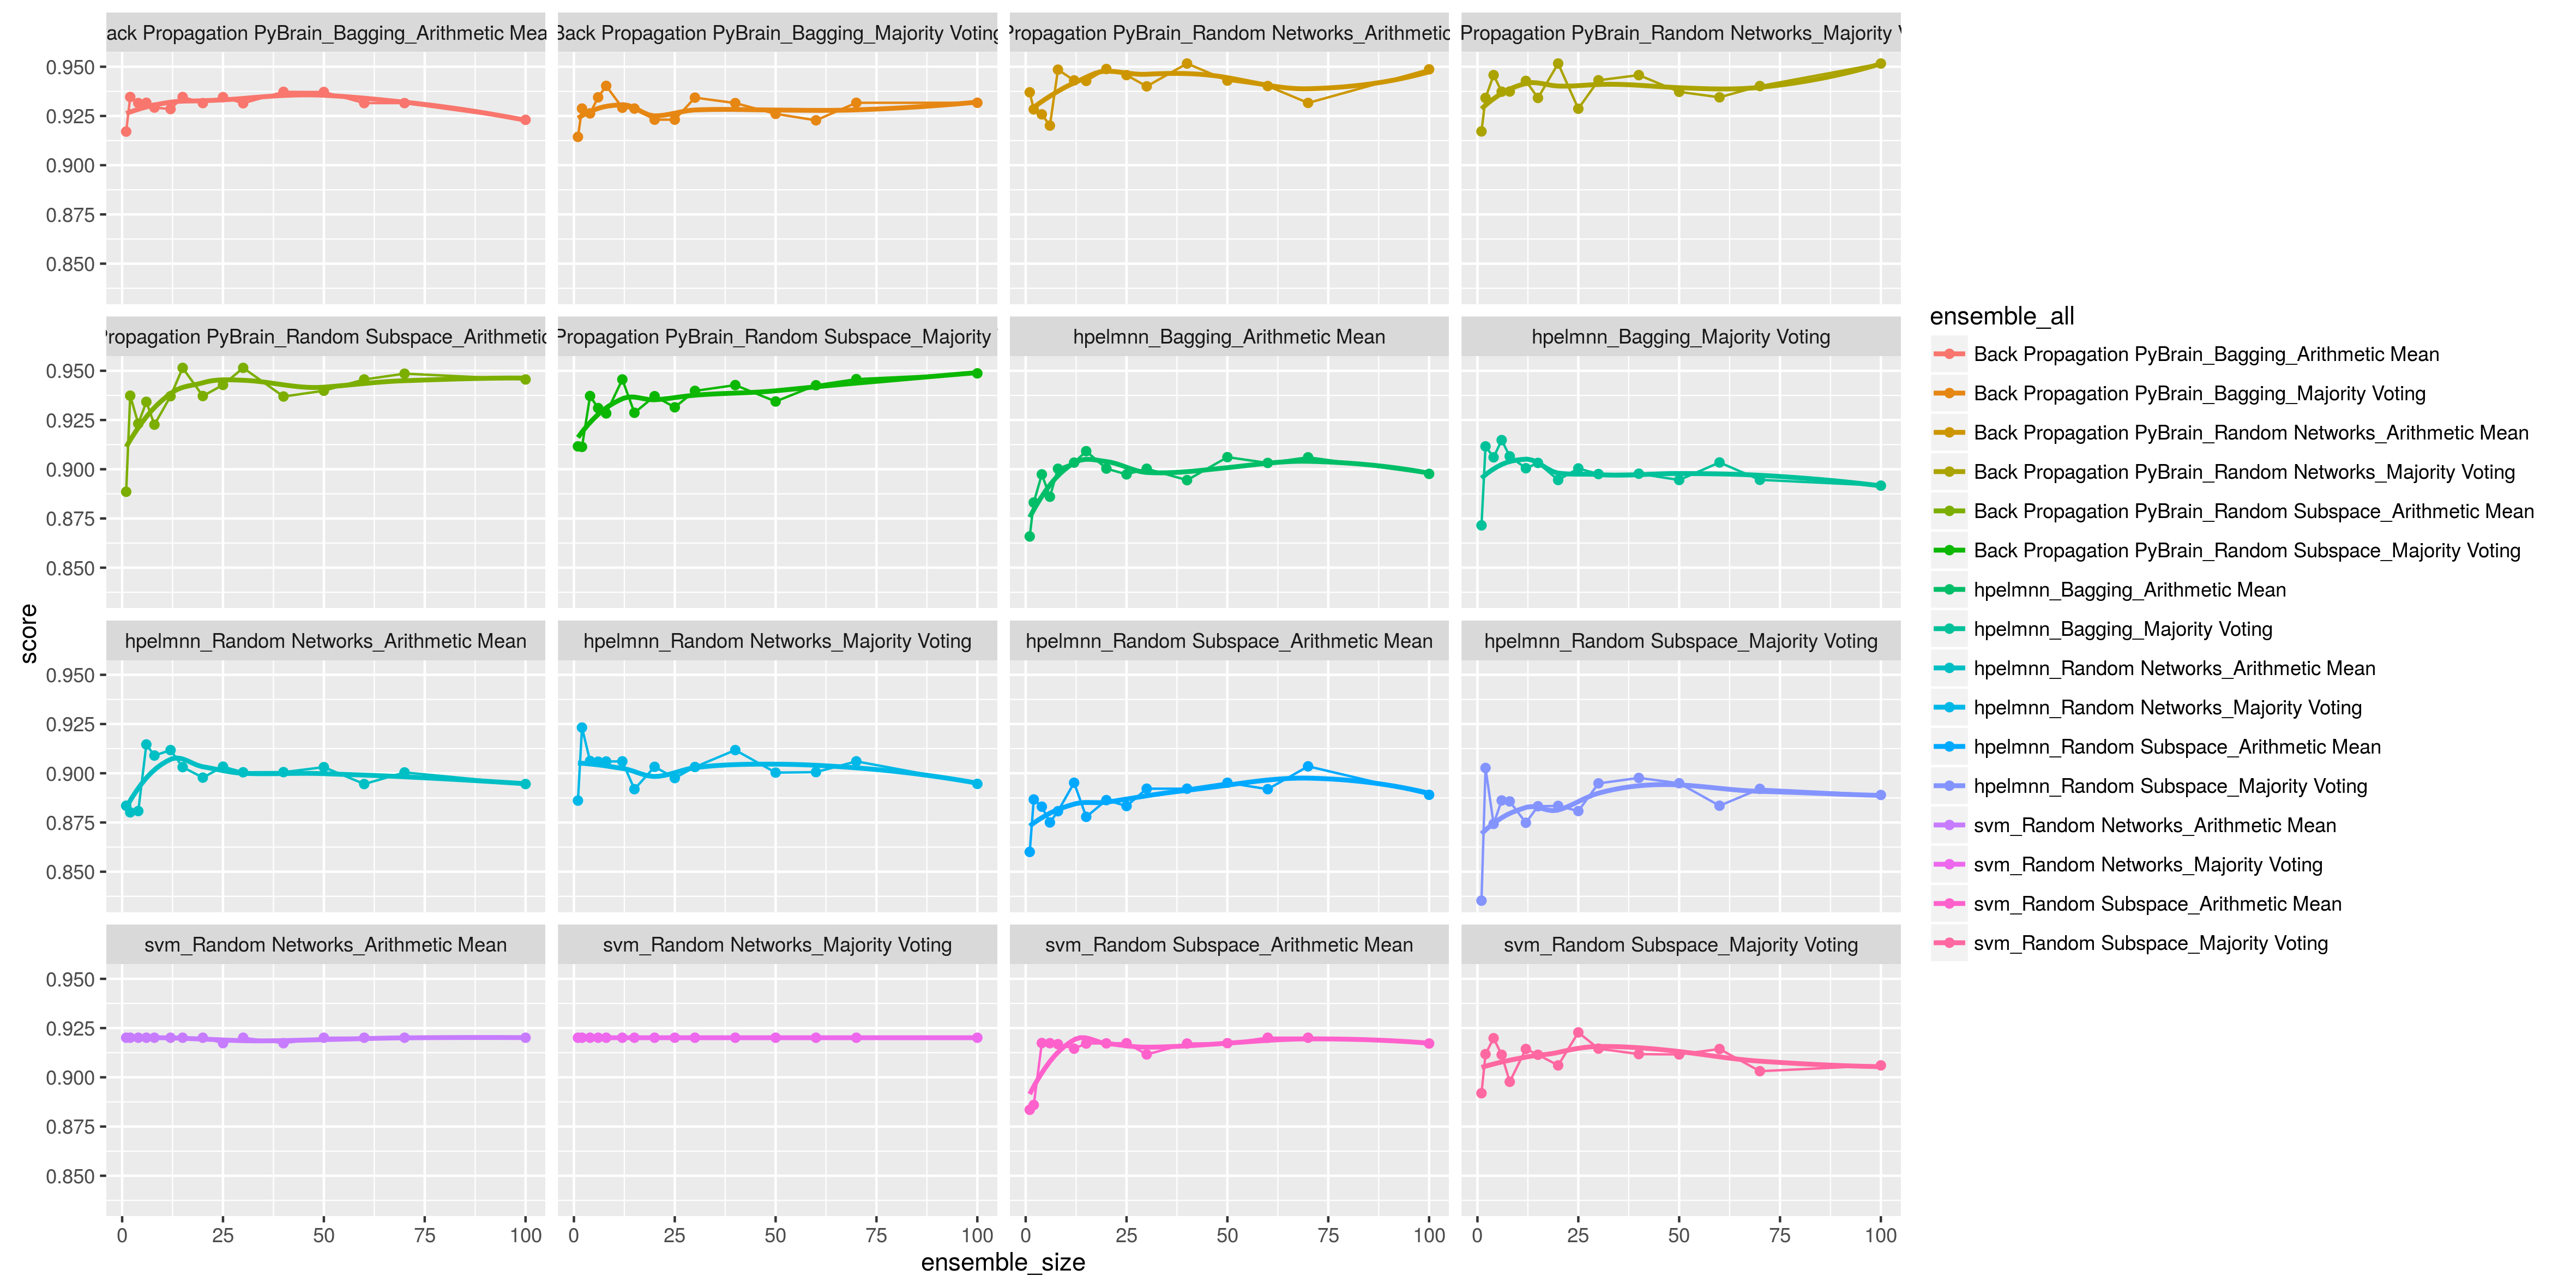
\includegraphics[width=1.0\textwidth]{type2_score_size_model_ionosphere}\centering\caption{ionosphere}\end{figure}
\begin{figure}[H]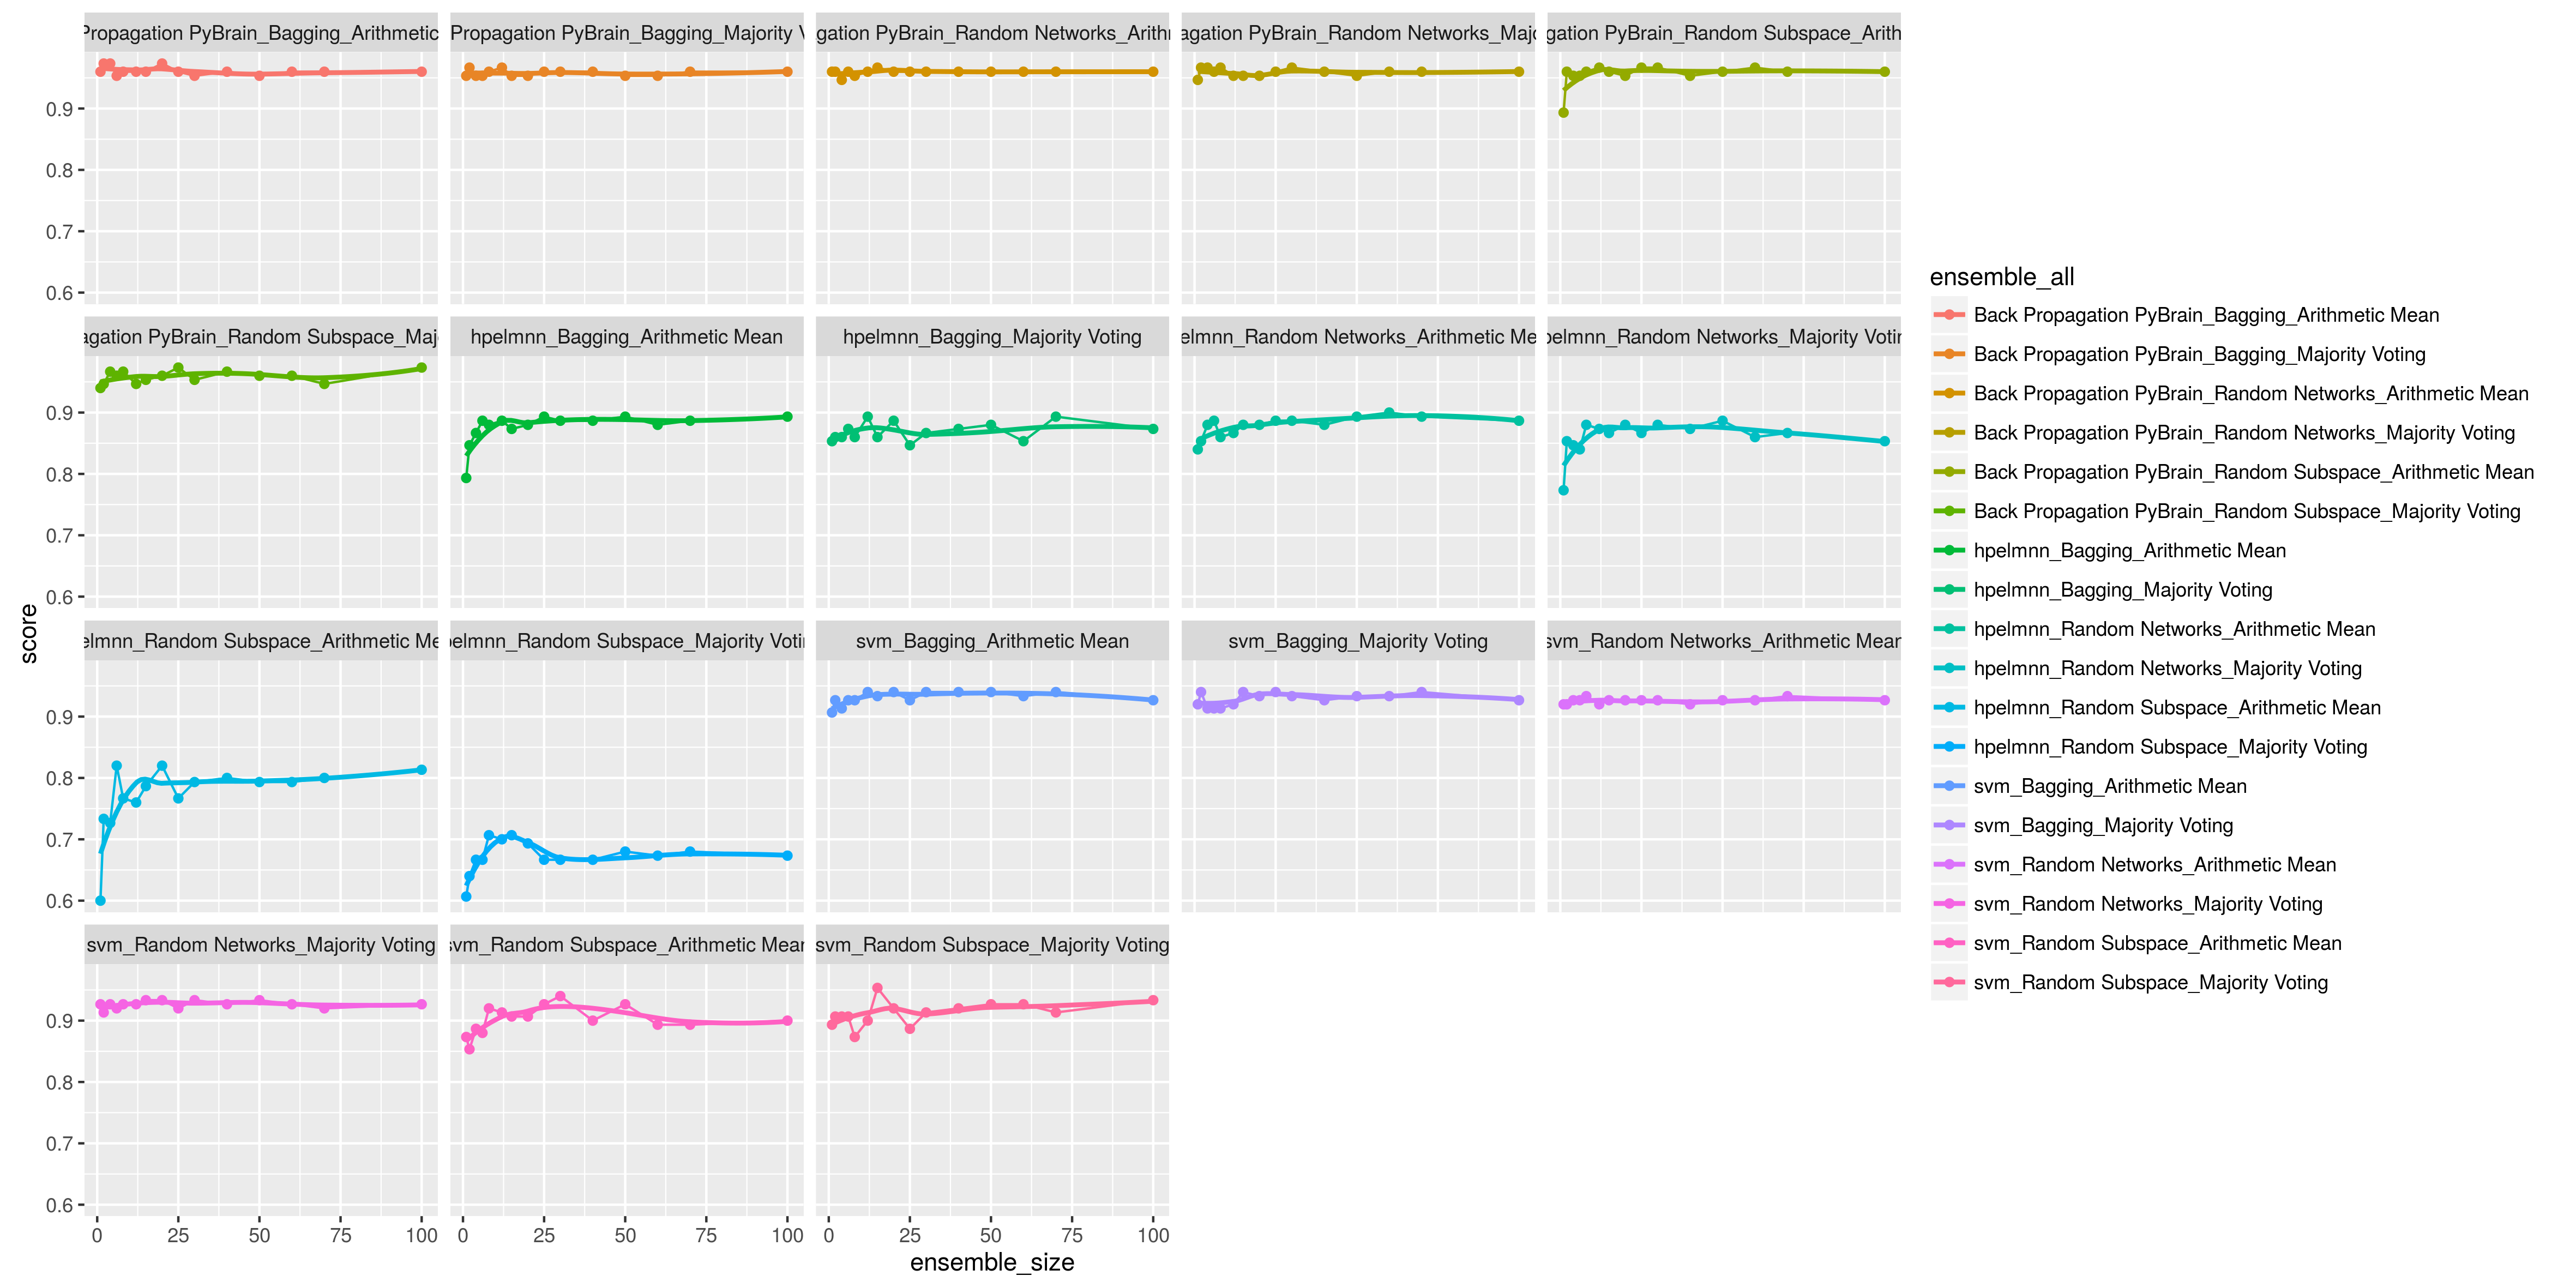
\includegraphics[width=1.0\textwidth]{type2_score_size_model_iris}\centering\caption{iris}\end{figure}
\begin{figure}[H]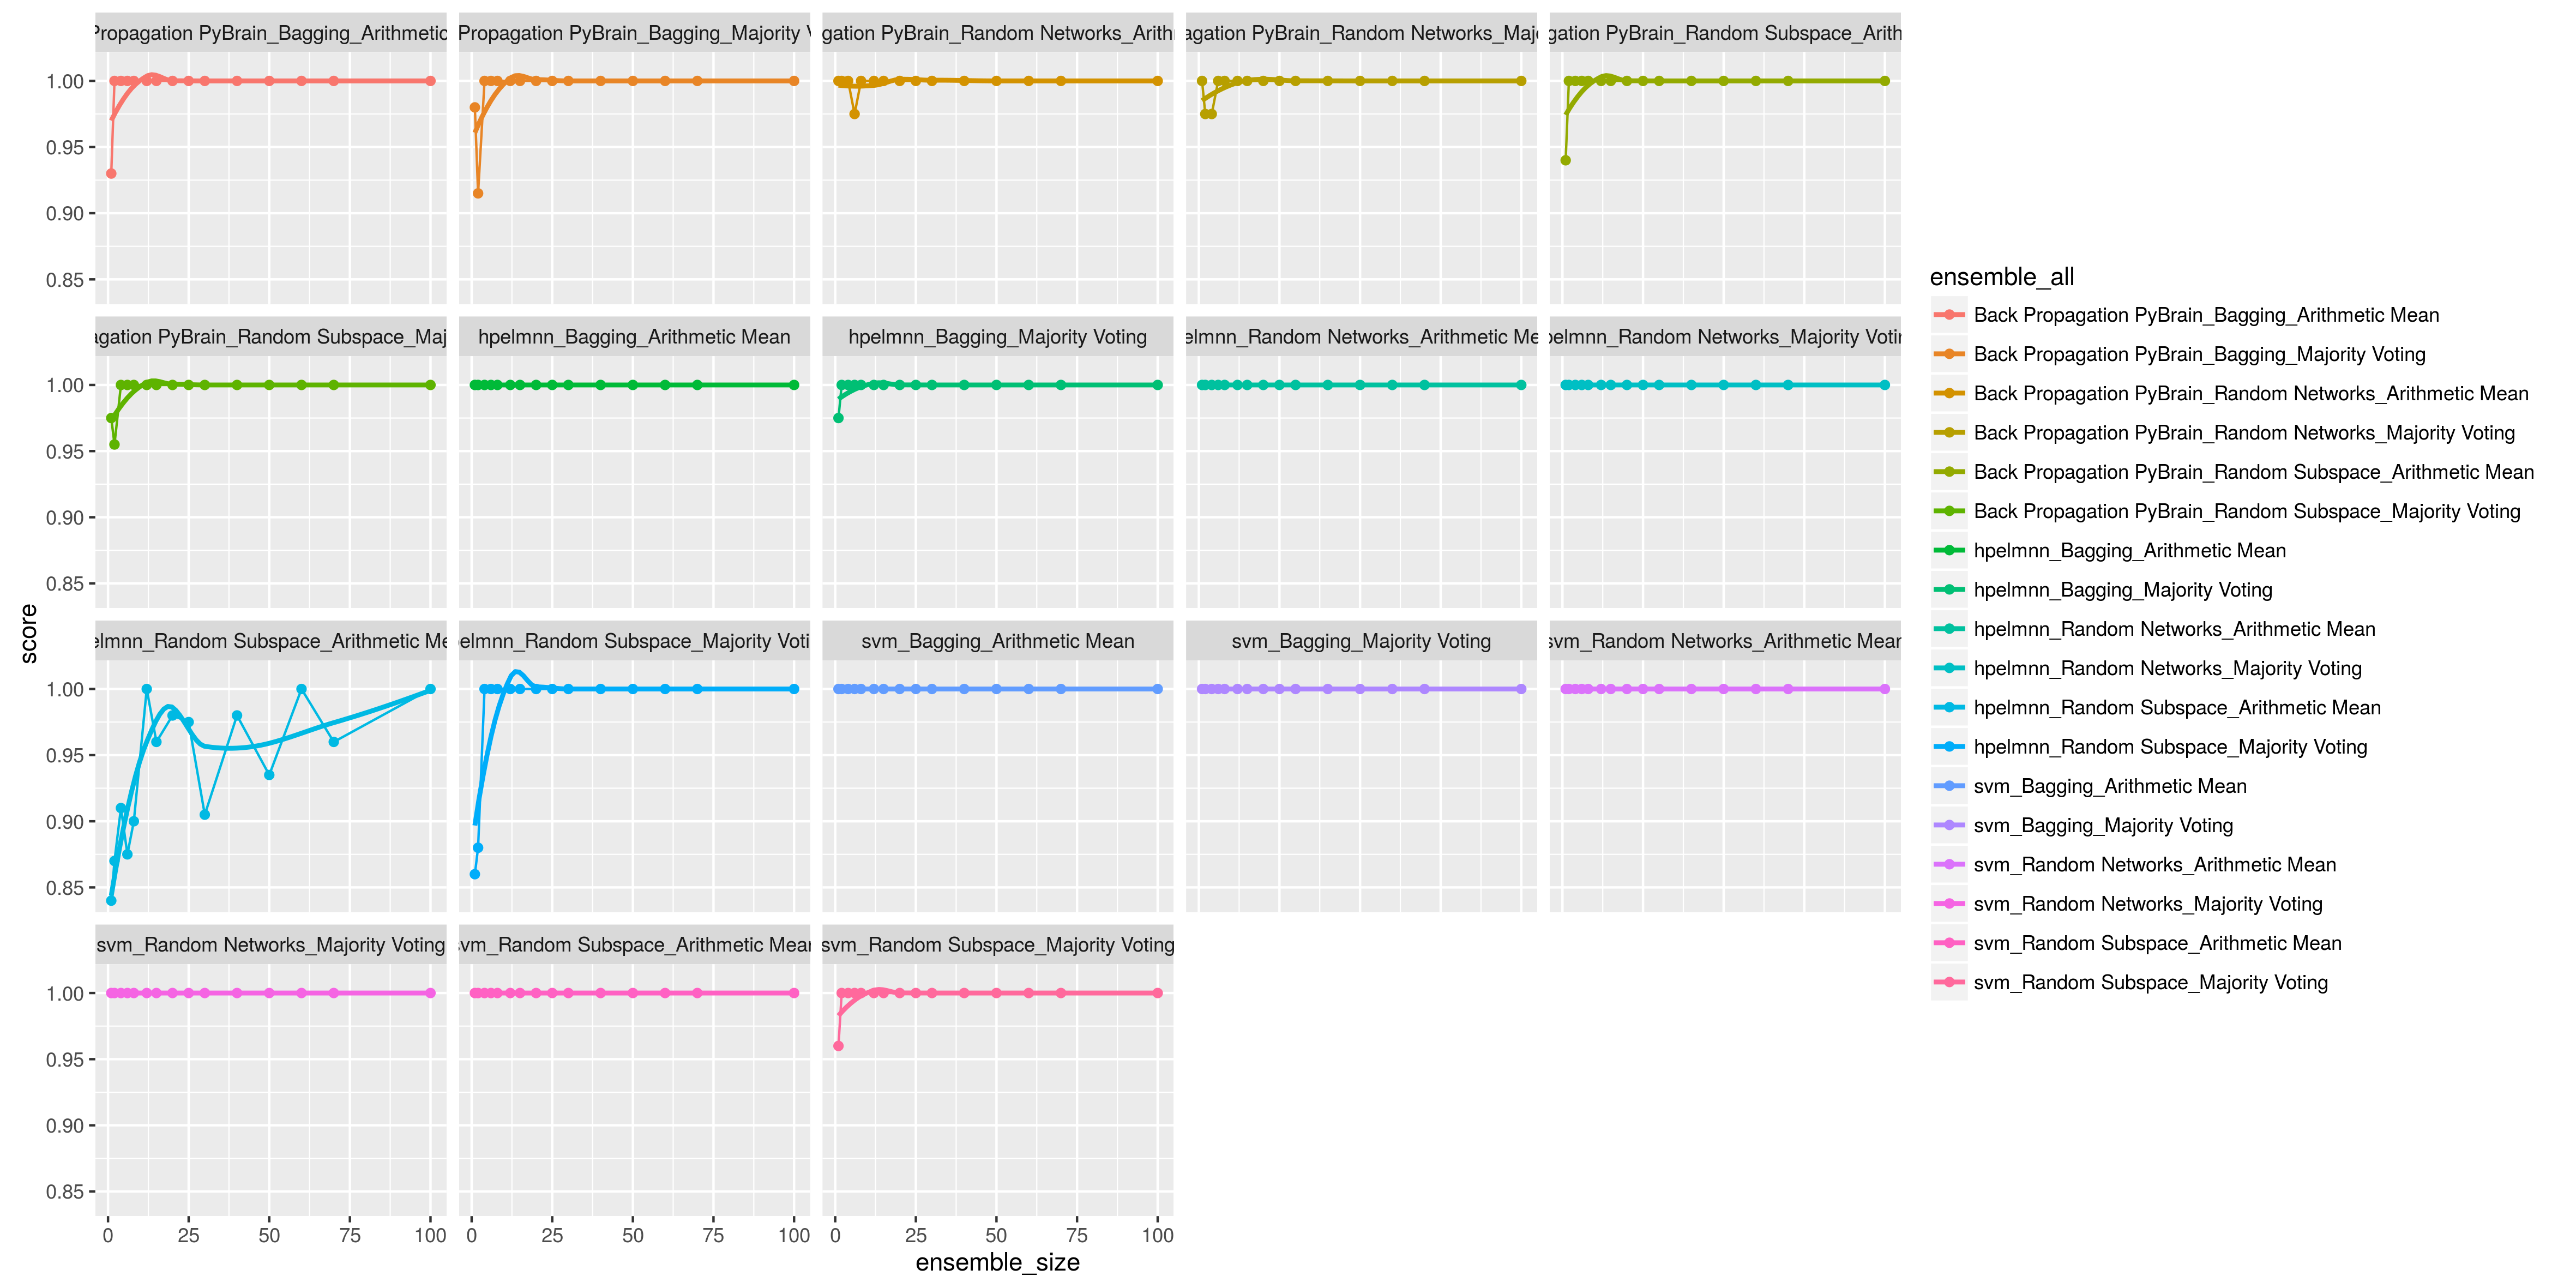
\includegraphics[width=1.0\textwidth]{type2_score_size_model_soybean_small}\centering\caption{soybean\_small}\end{figure}
\begin{figure}[H]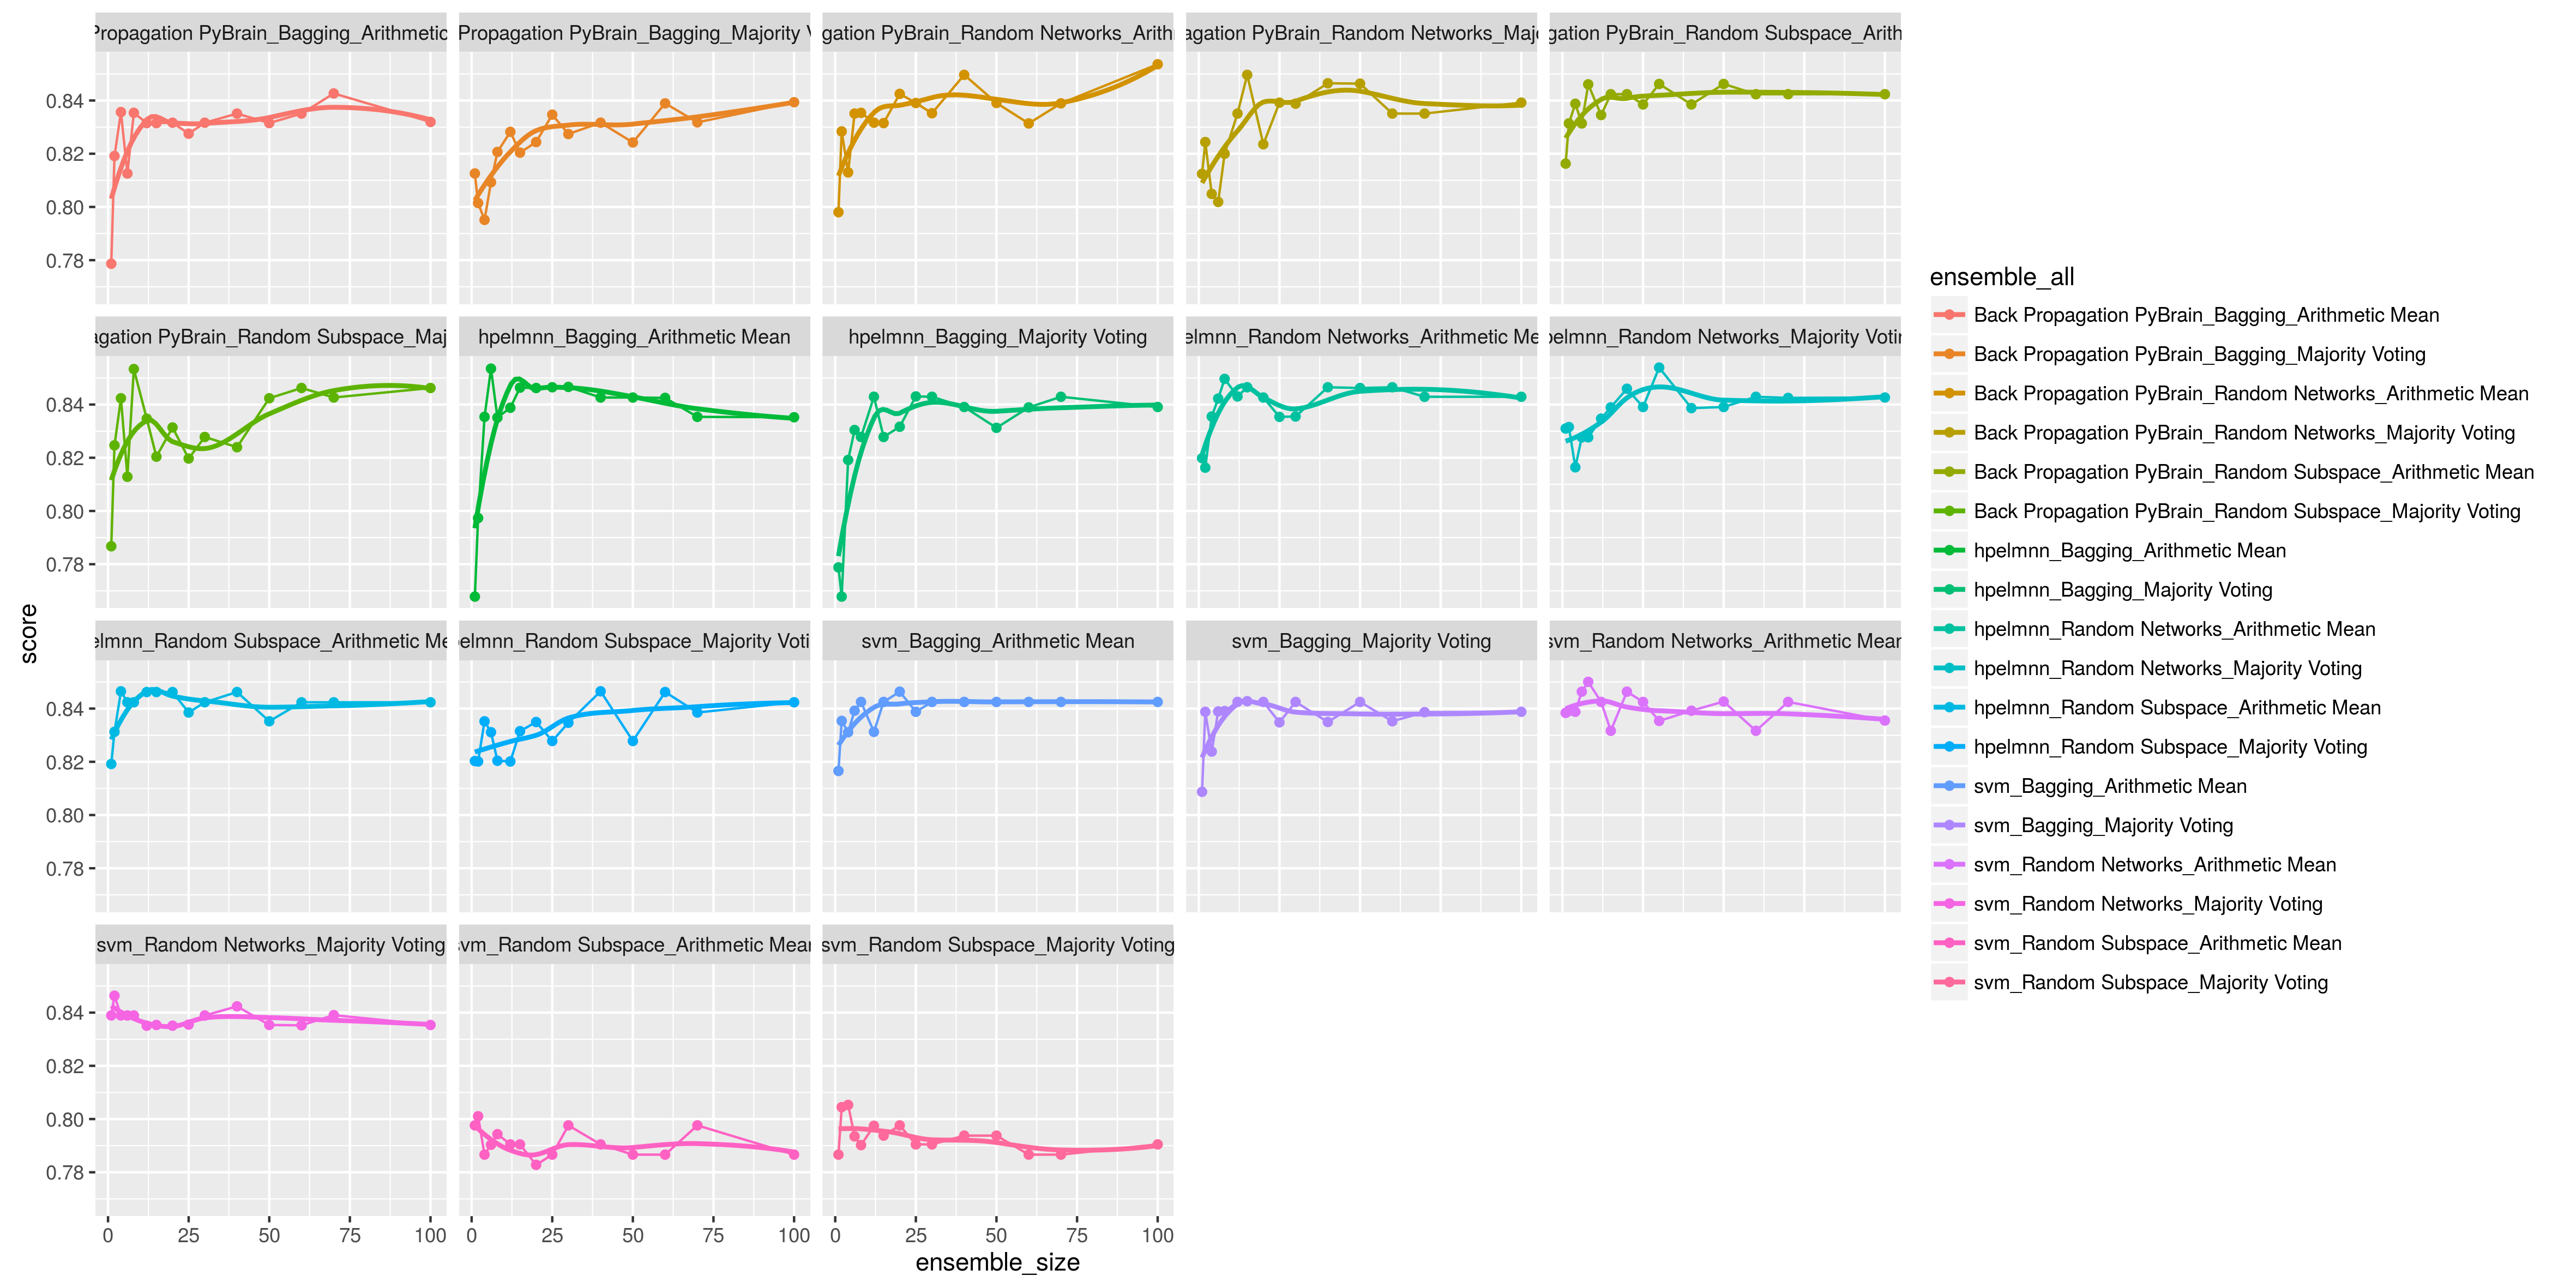
\includegraphics[width=1.0\textwidth]{type2_score_size_model_spect}\centering\caption{spect}\end{figure}
\begin{figure}[H]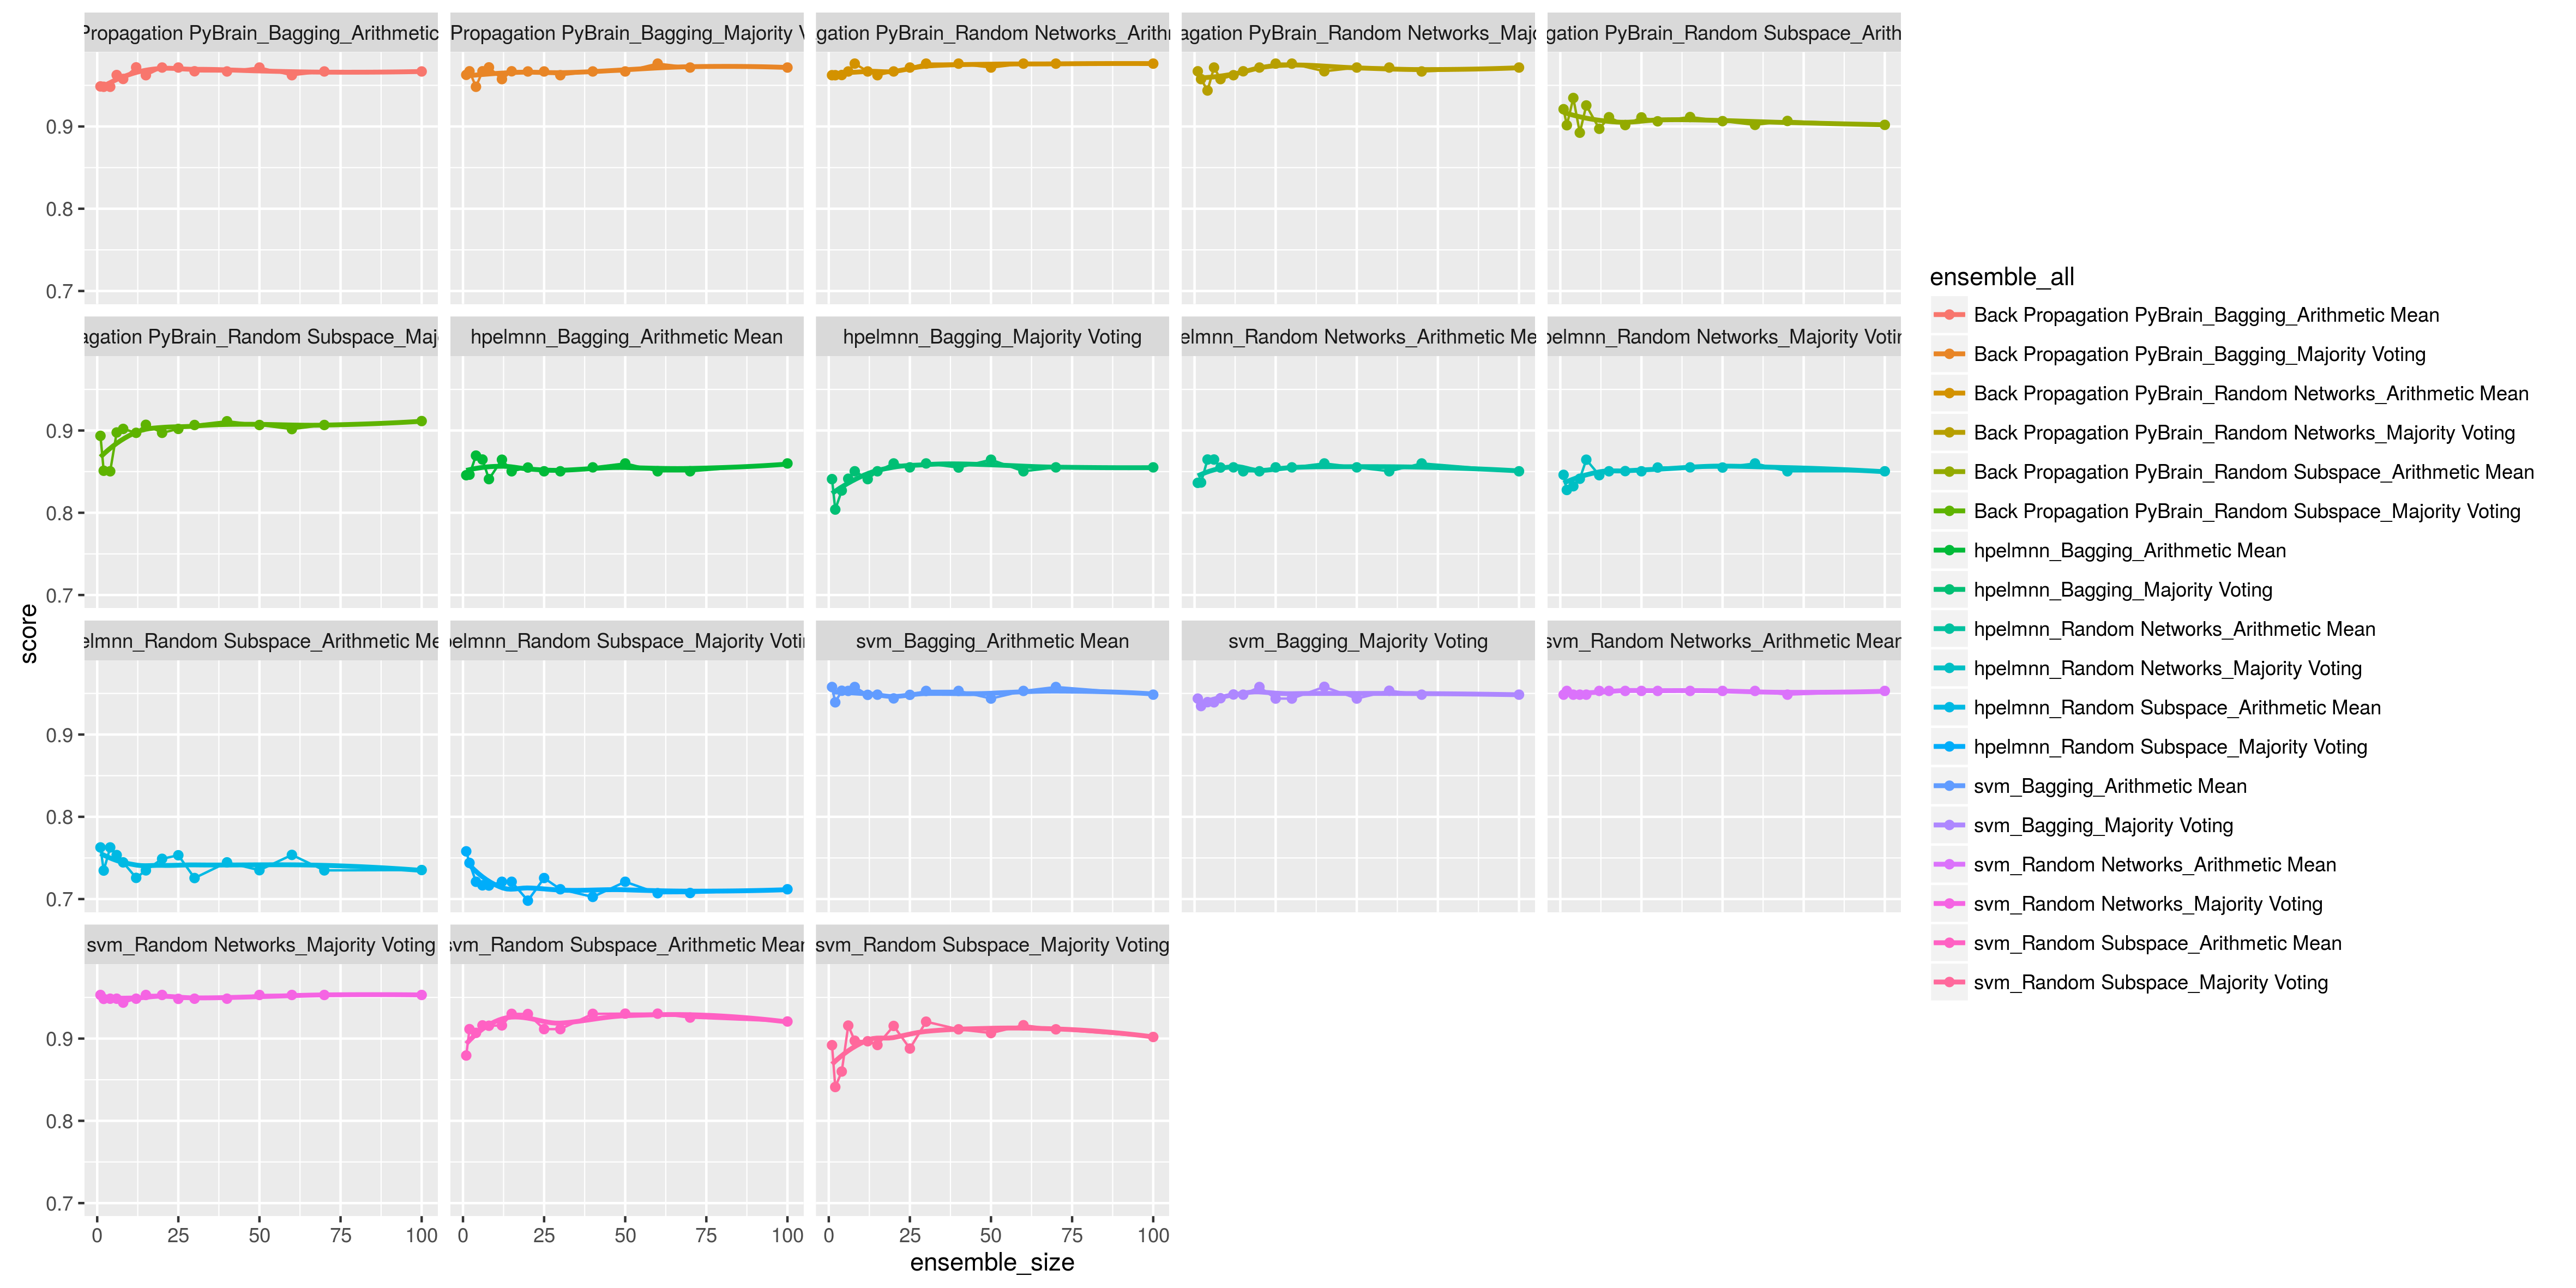
\includegraphics[width=1.0\textwidth]{type2_score_size_model_thyroid}\centering\caption{thyroid}\end{figure}
\begin{figure}[H]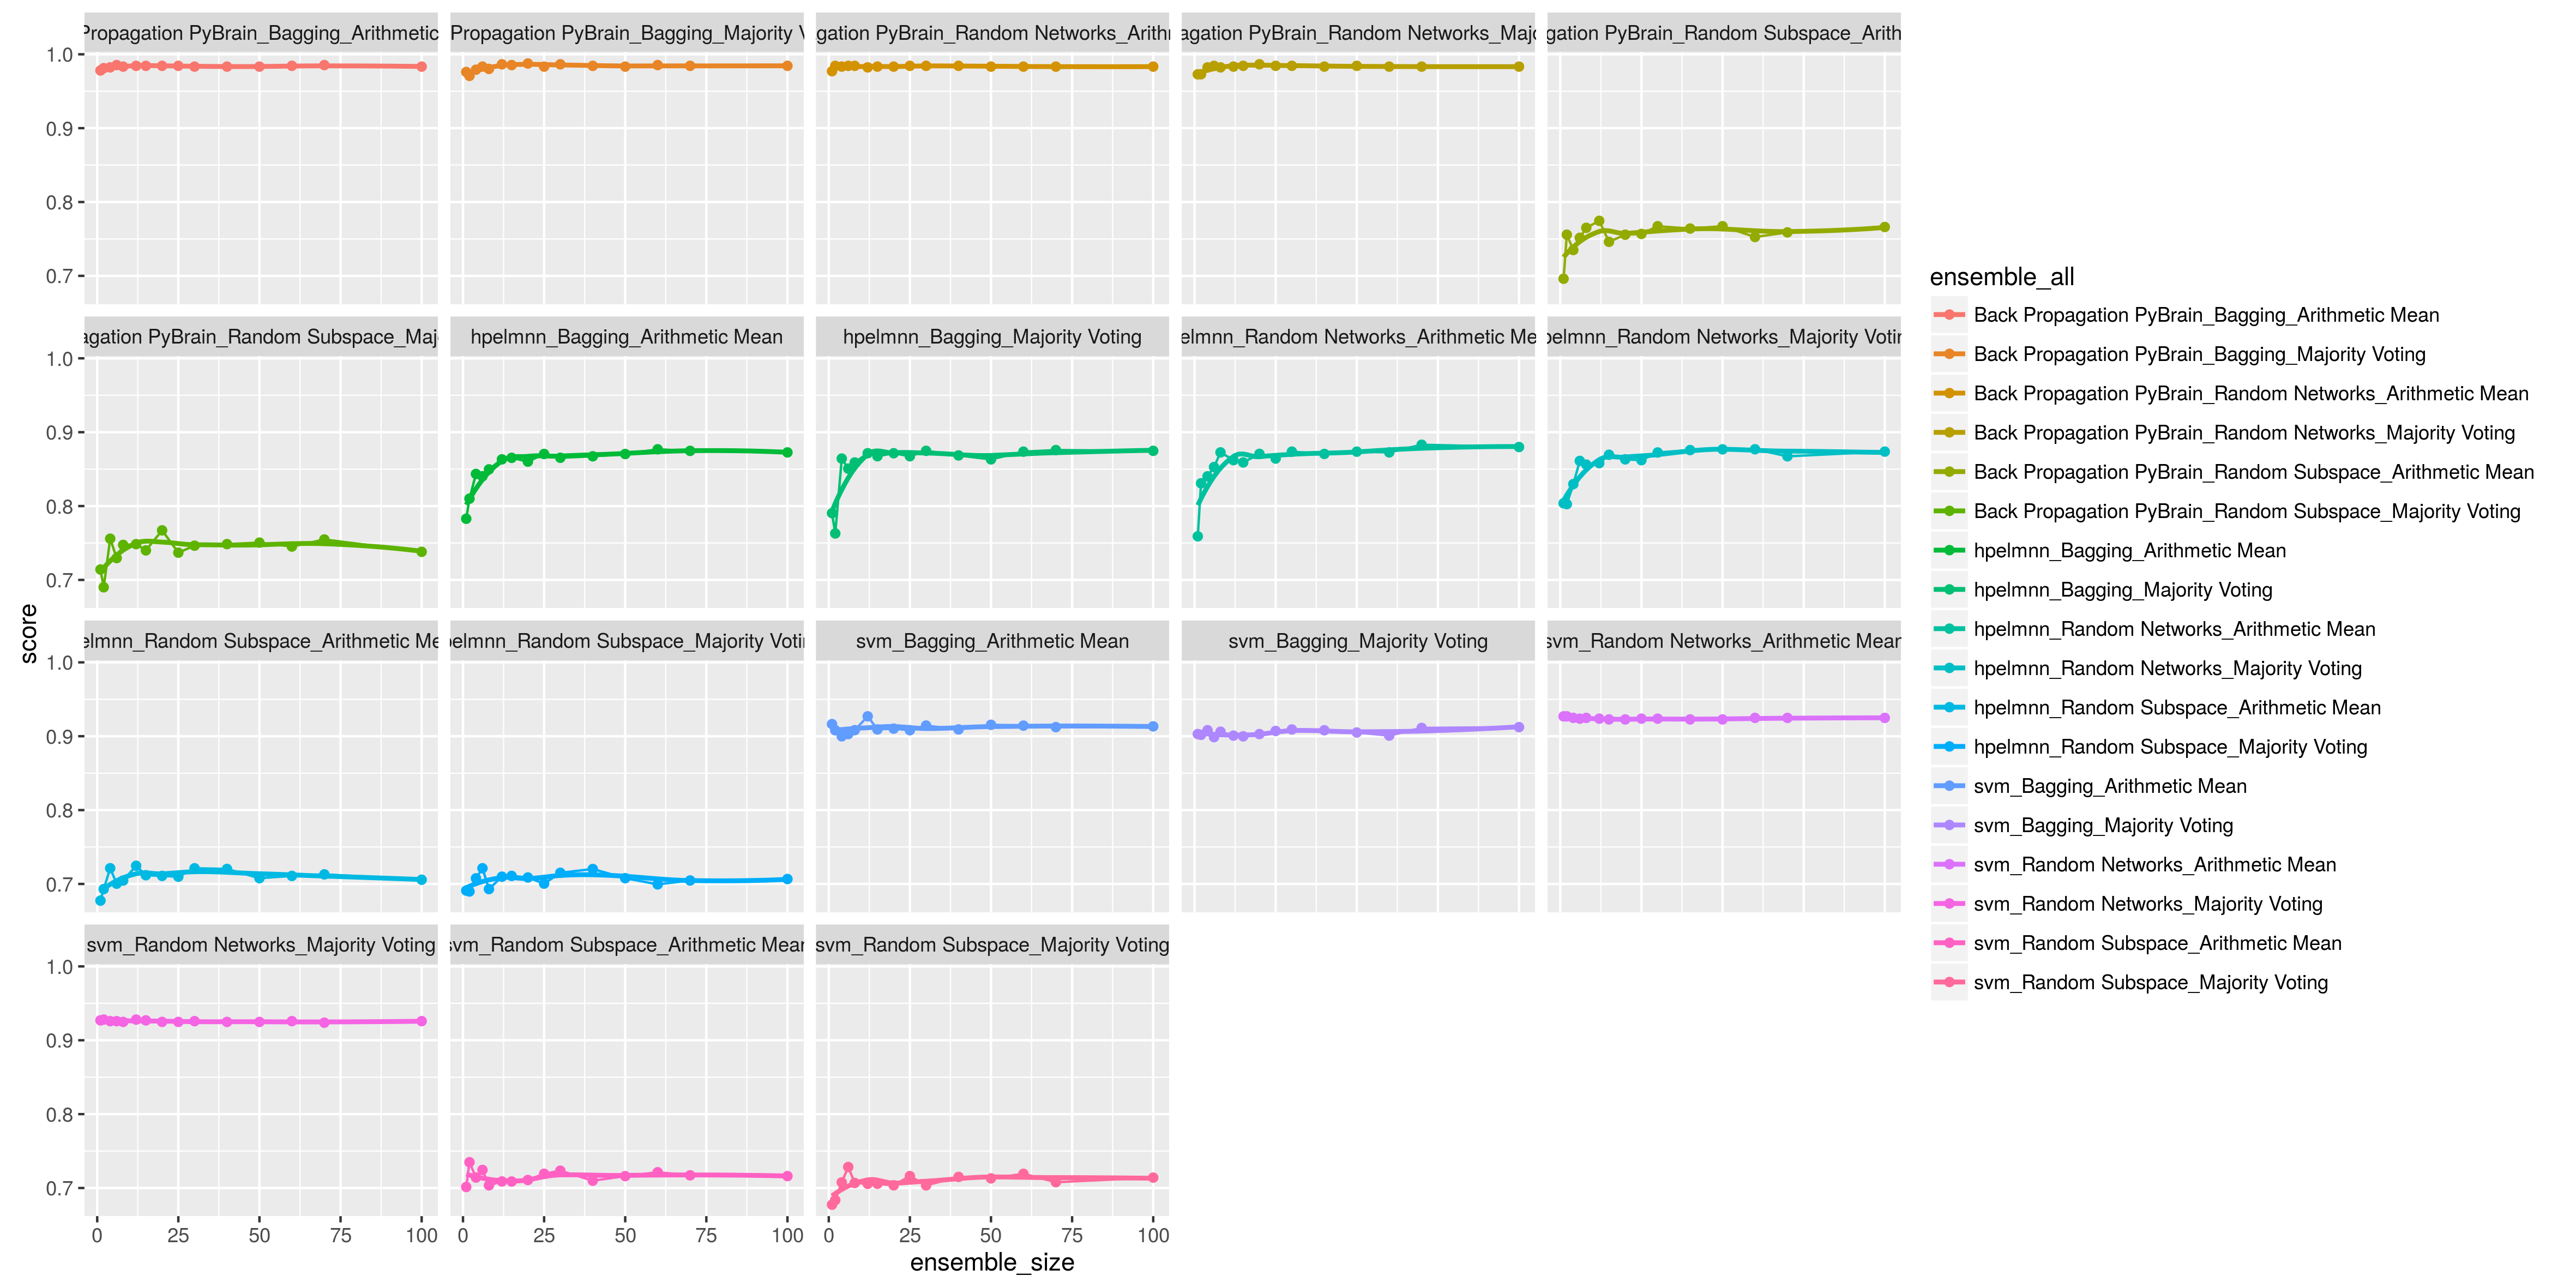
\includegraphics[width=1.0\textwidth]{type2_score_size_model_tic_tac_toe}\centering\caption{tic\_tac\_toe}\end{figure}
\begin{figure}[H]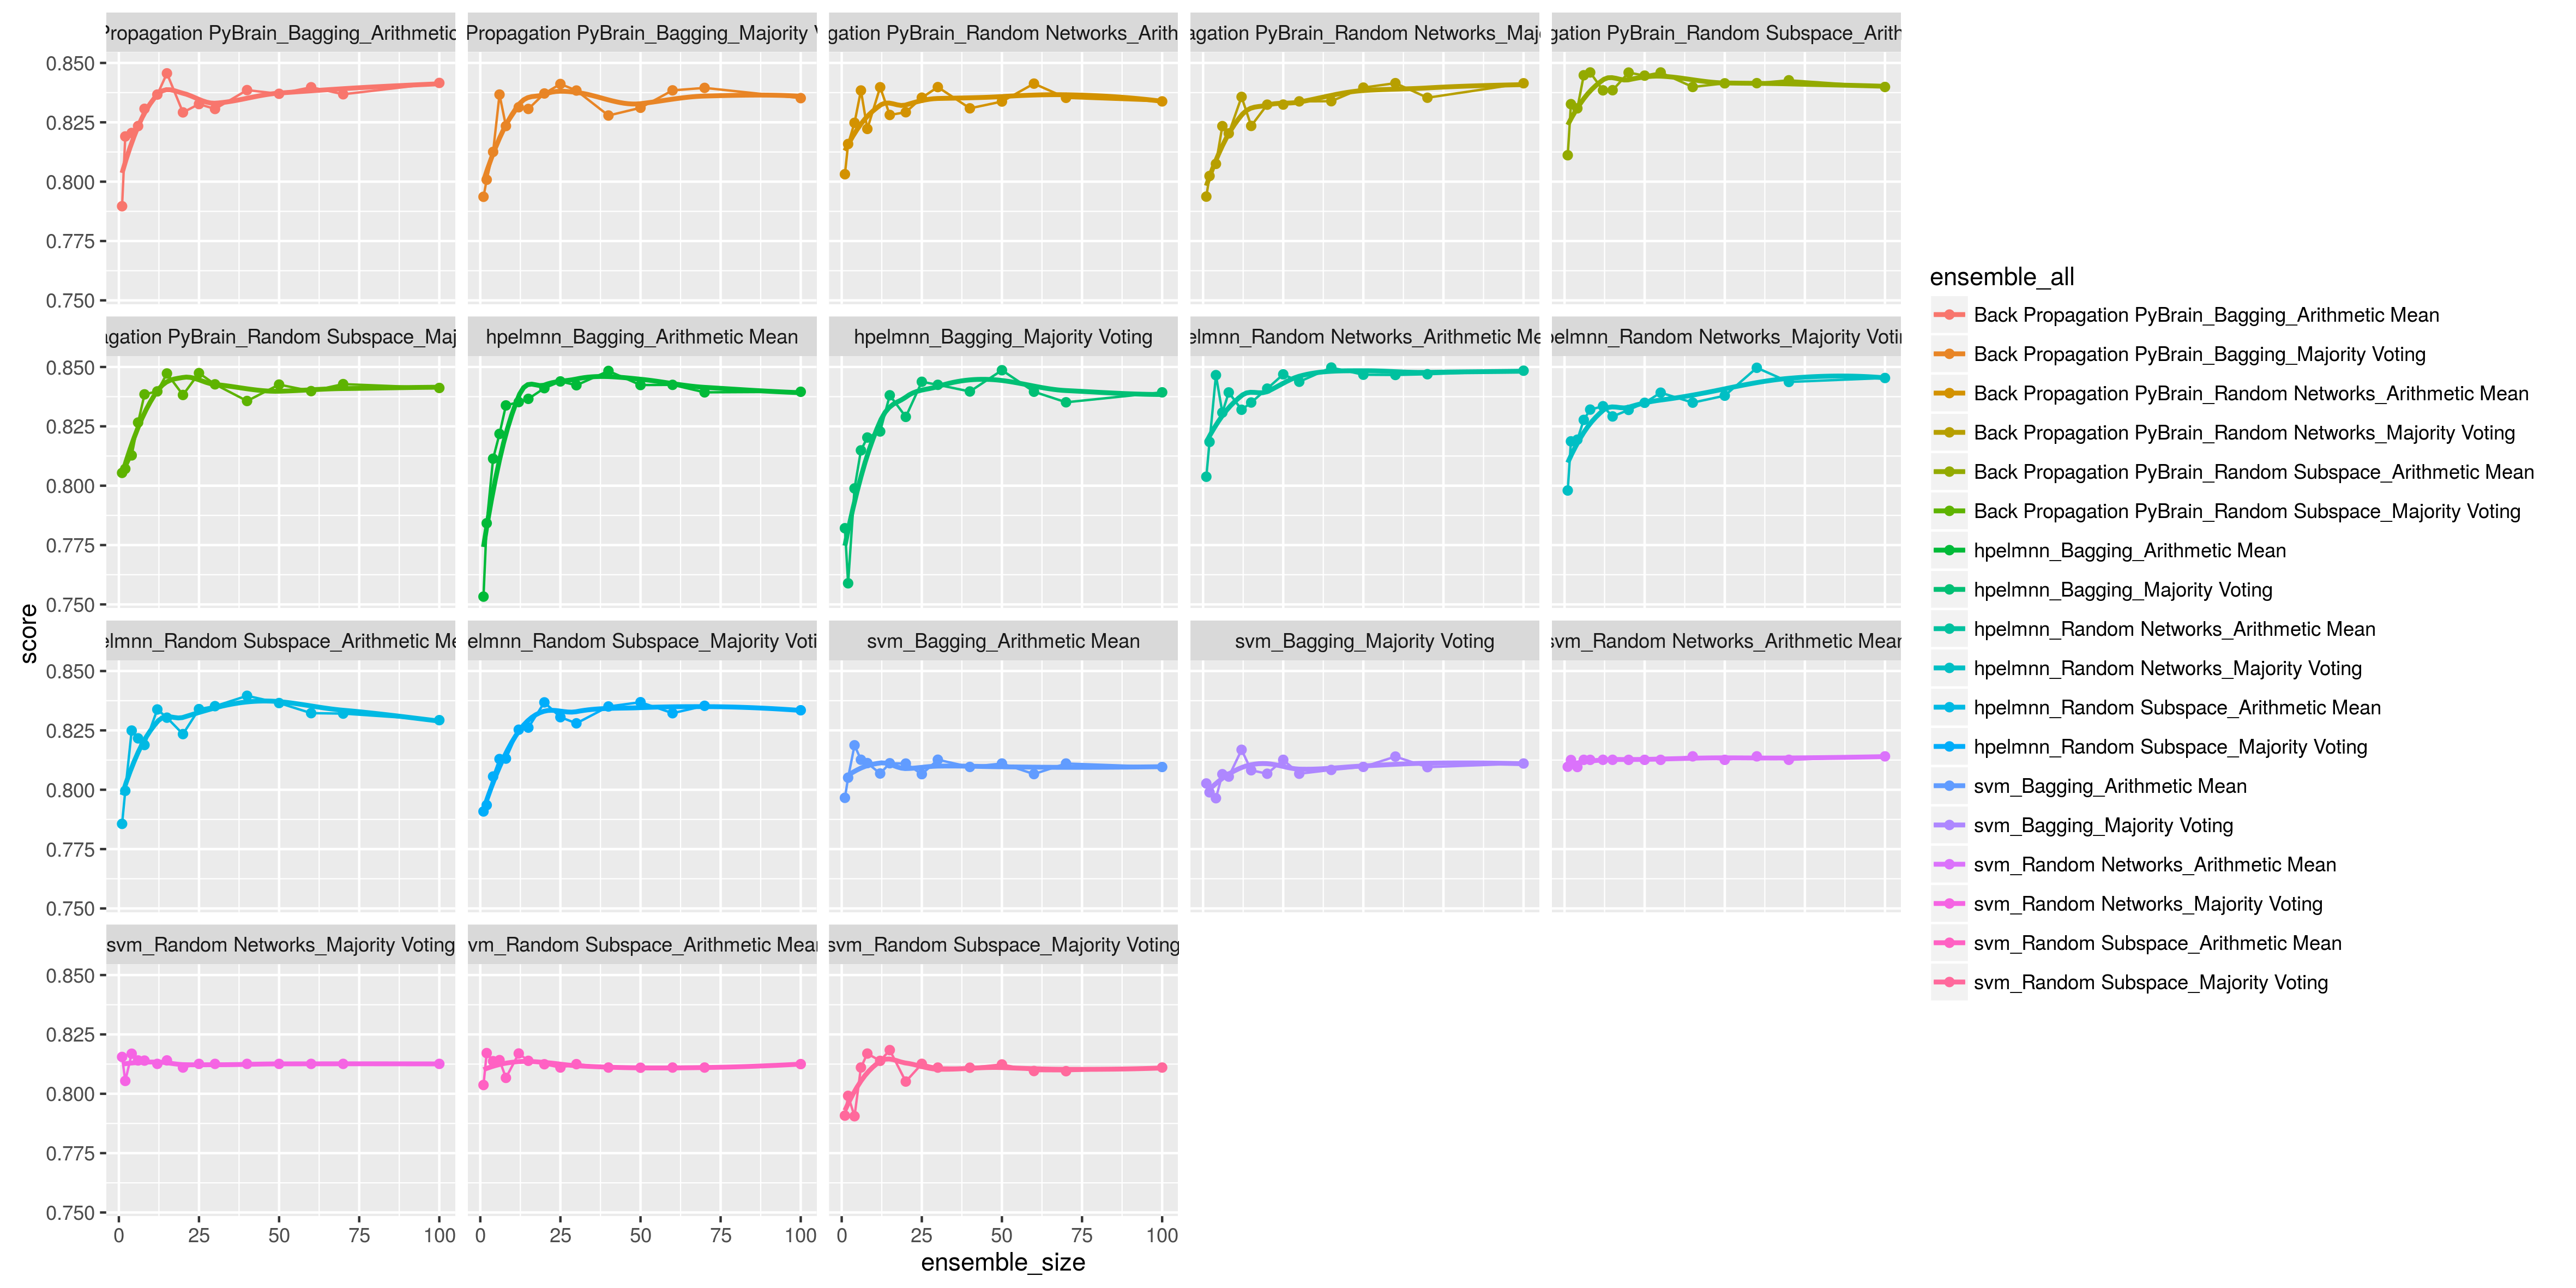
\includegraphics[width=1.0\textwidth]{type2_score_size_model_urban_land_cover}\centering\caption{urban\_land\_cover}\end{figure}
\begin{figure}[H]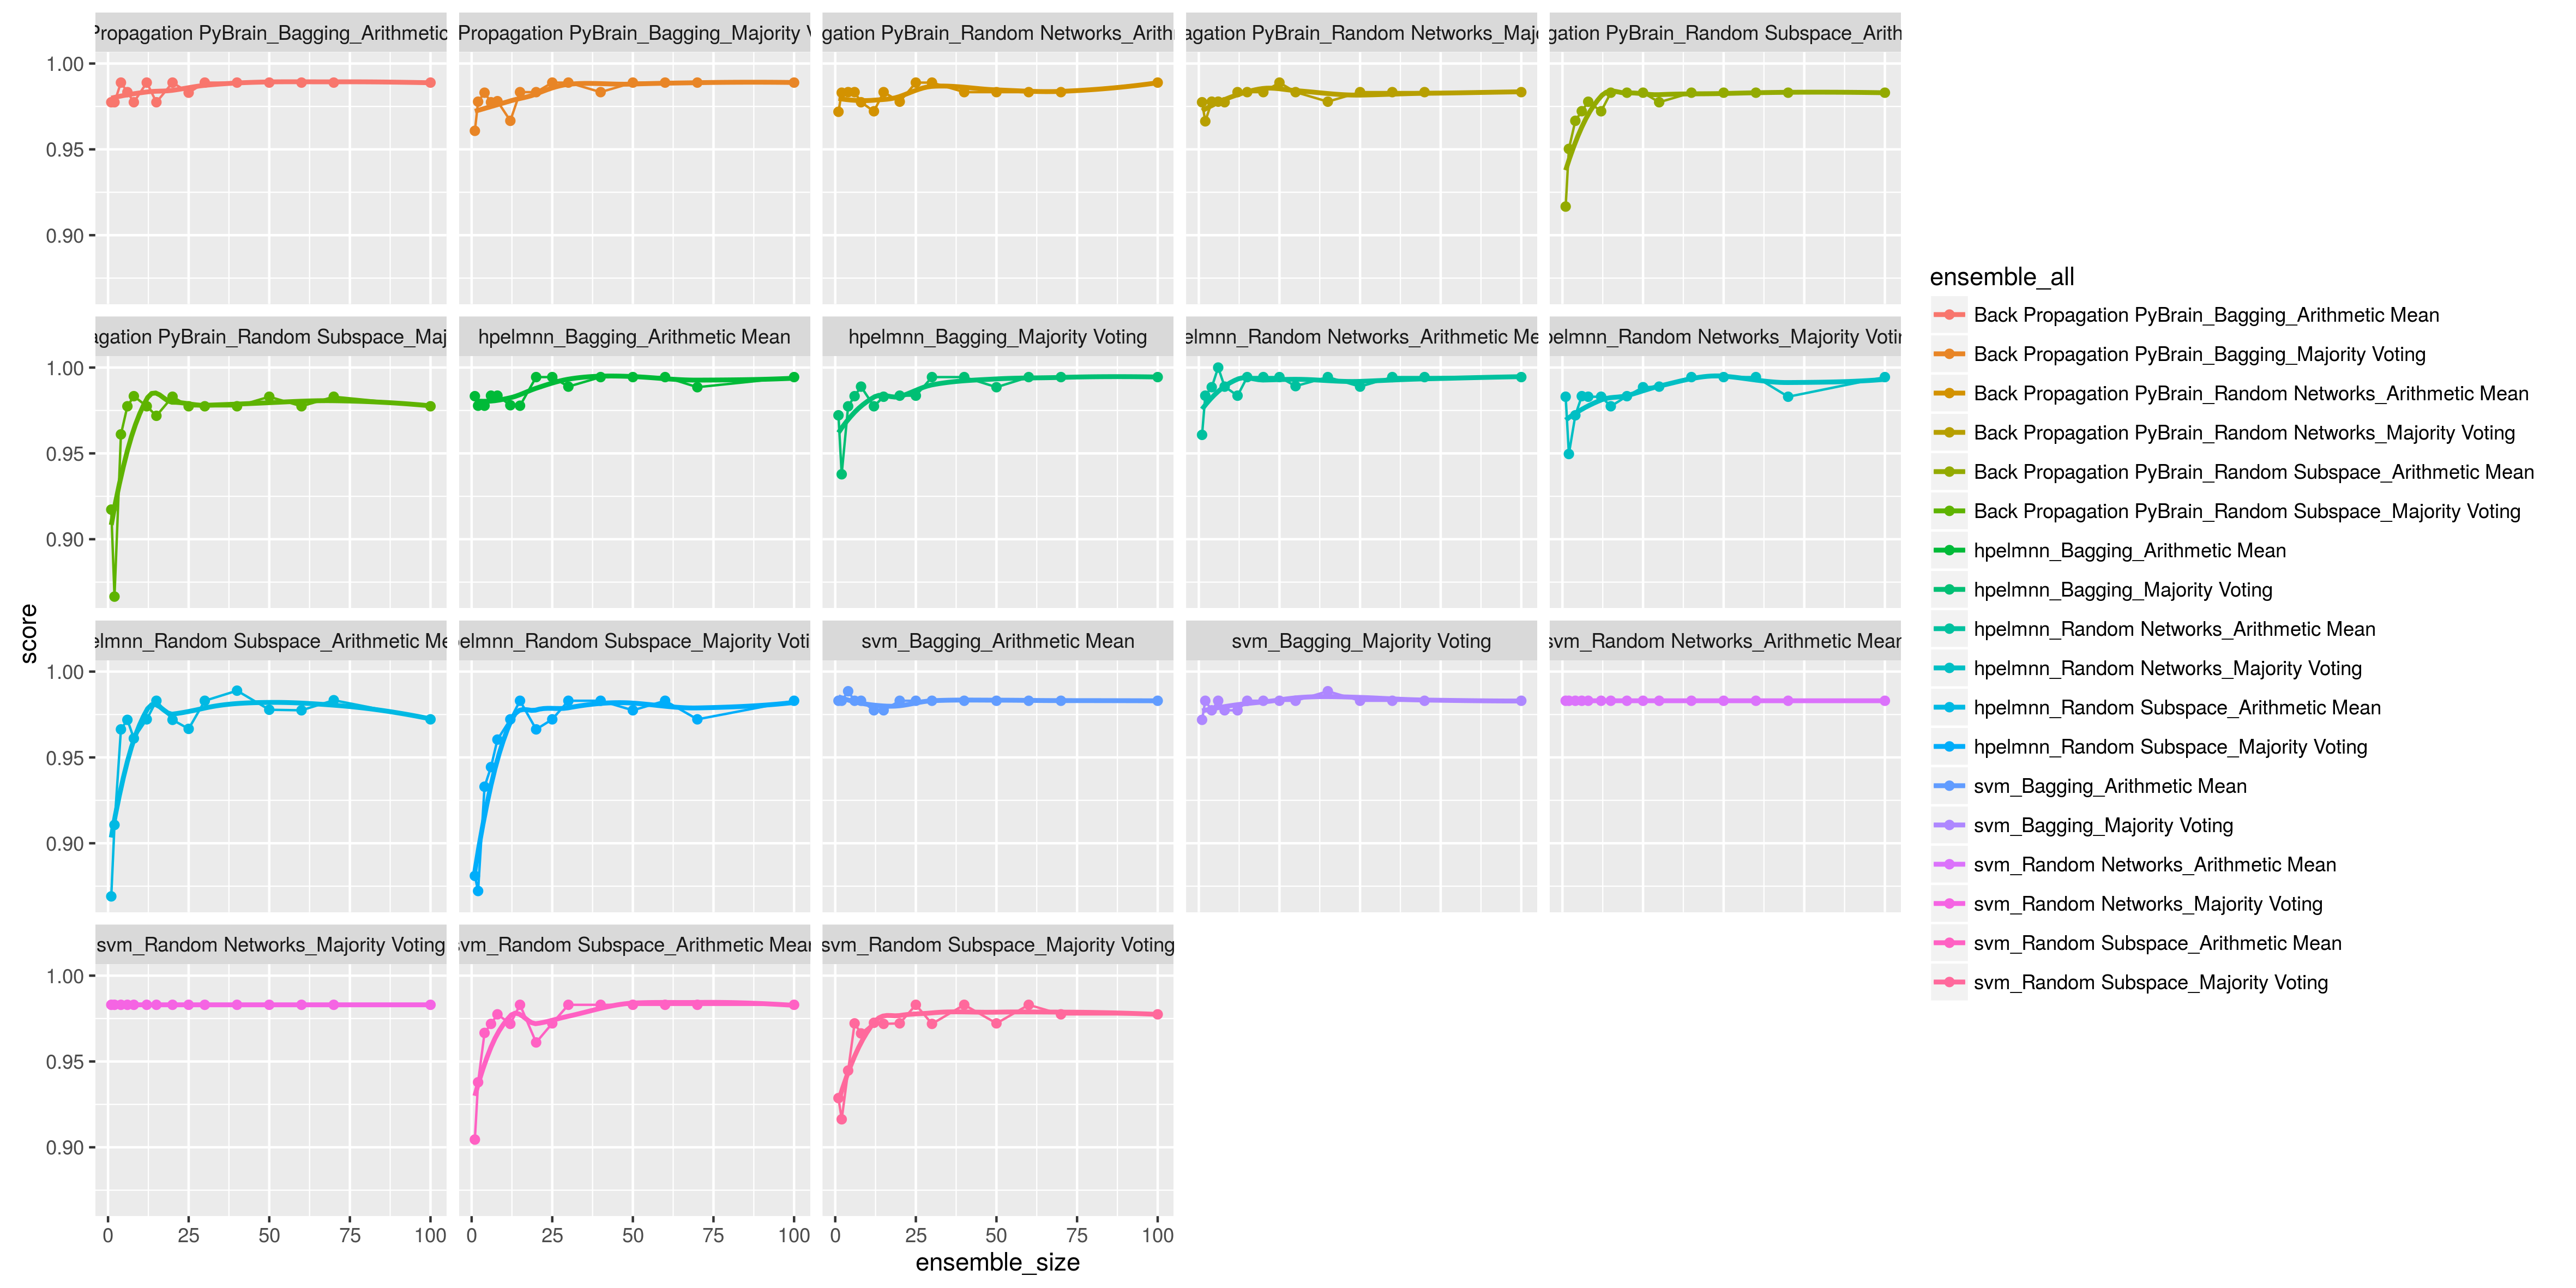
\includegraphics[width=1.0\textwidth]{type2_score_size_model_wine}\centering\caption{wine}\end{figure}
\begin{figure}[H]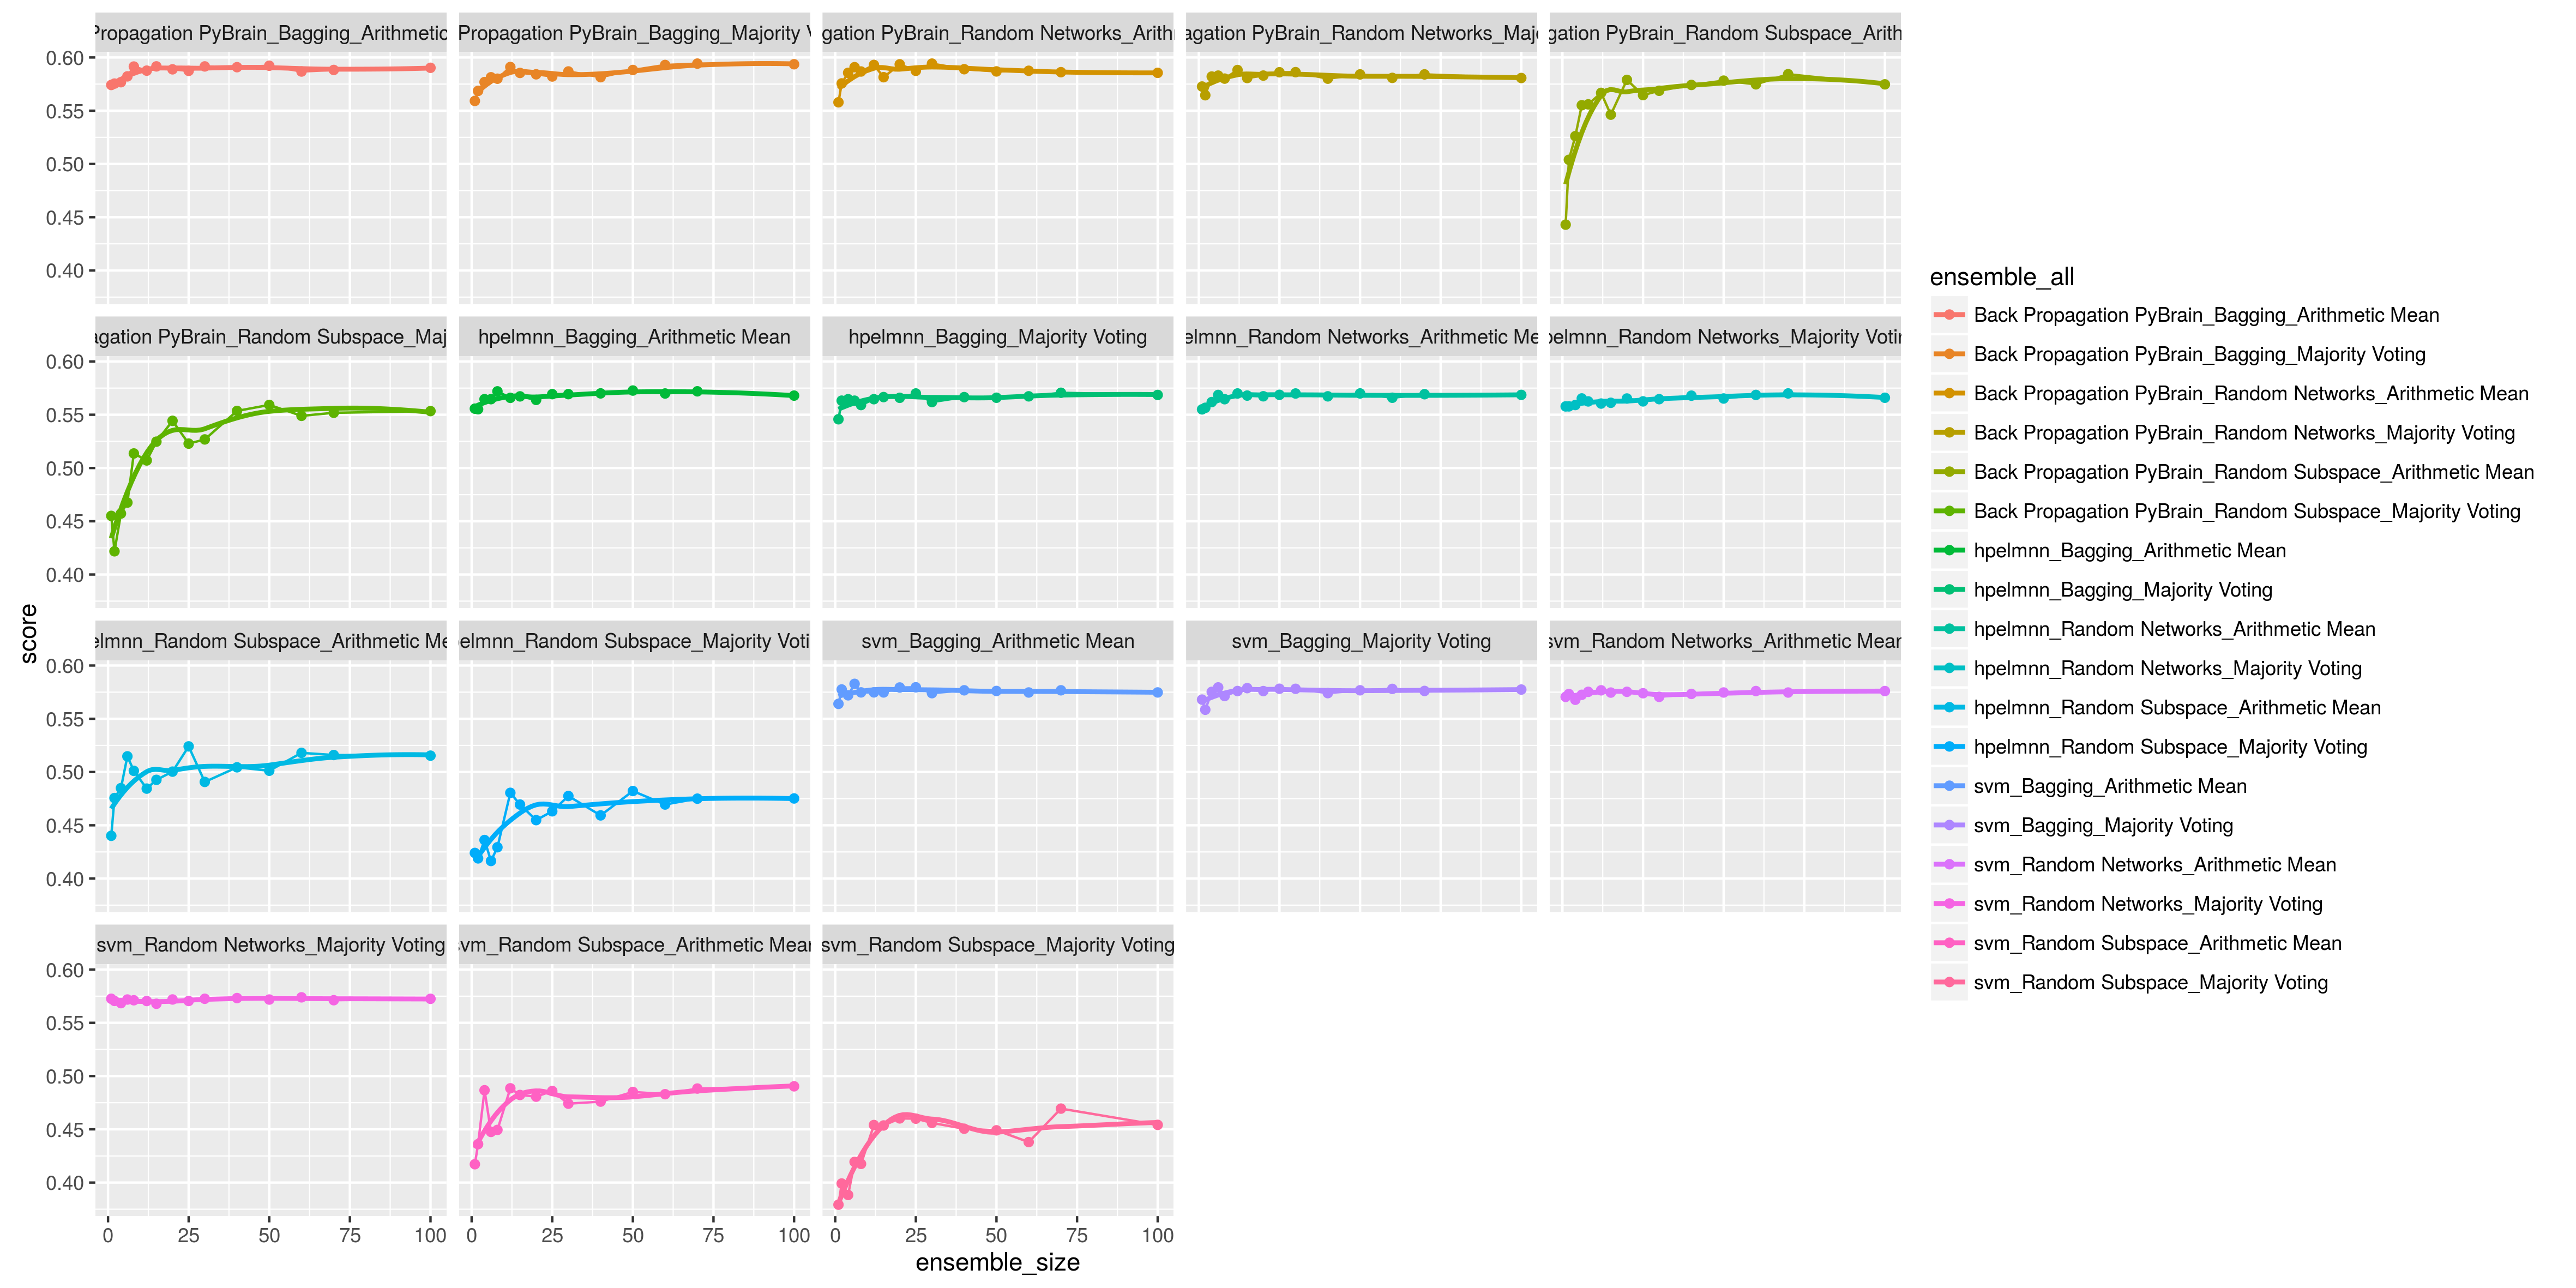
\includegraphics[width=1.0\textwidth]{type2_score_size_model_yeast}\centering\caption{yeast}\end{figure}

\begin{figure}[H]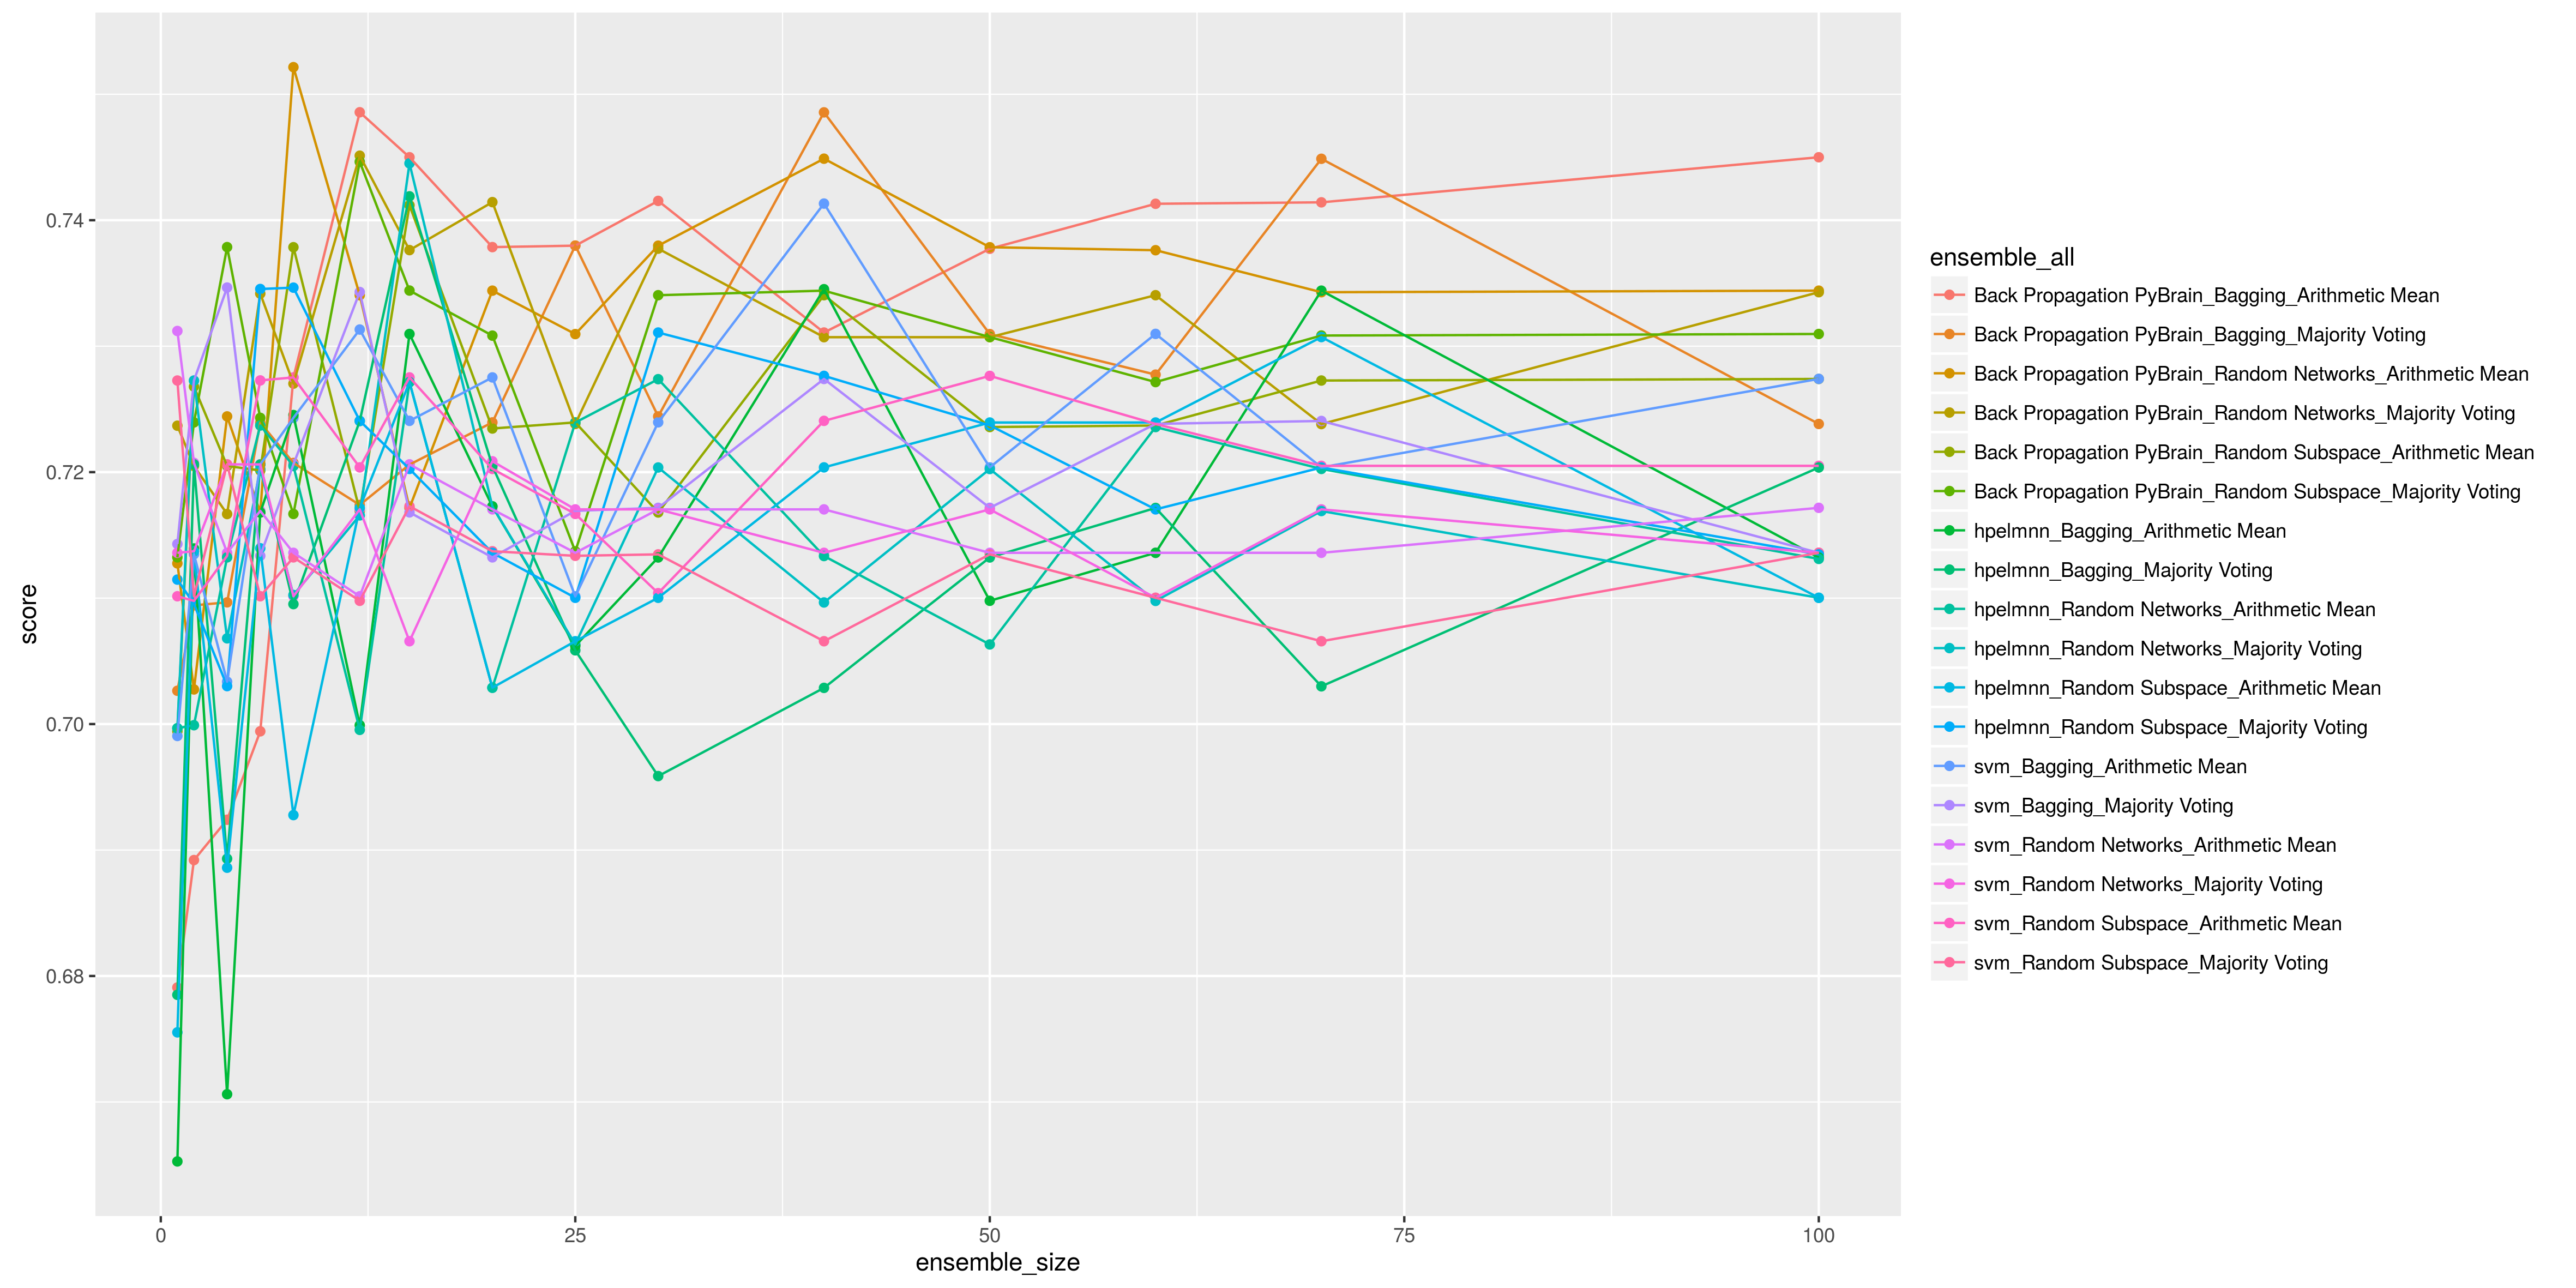
\includegraphics[width=1.0\textwidth]{type3_score_size_dataset_breast_cancer}\centering\caption{breast\_cancer}\end{figure}
\begin{figure}[H]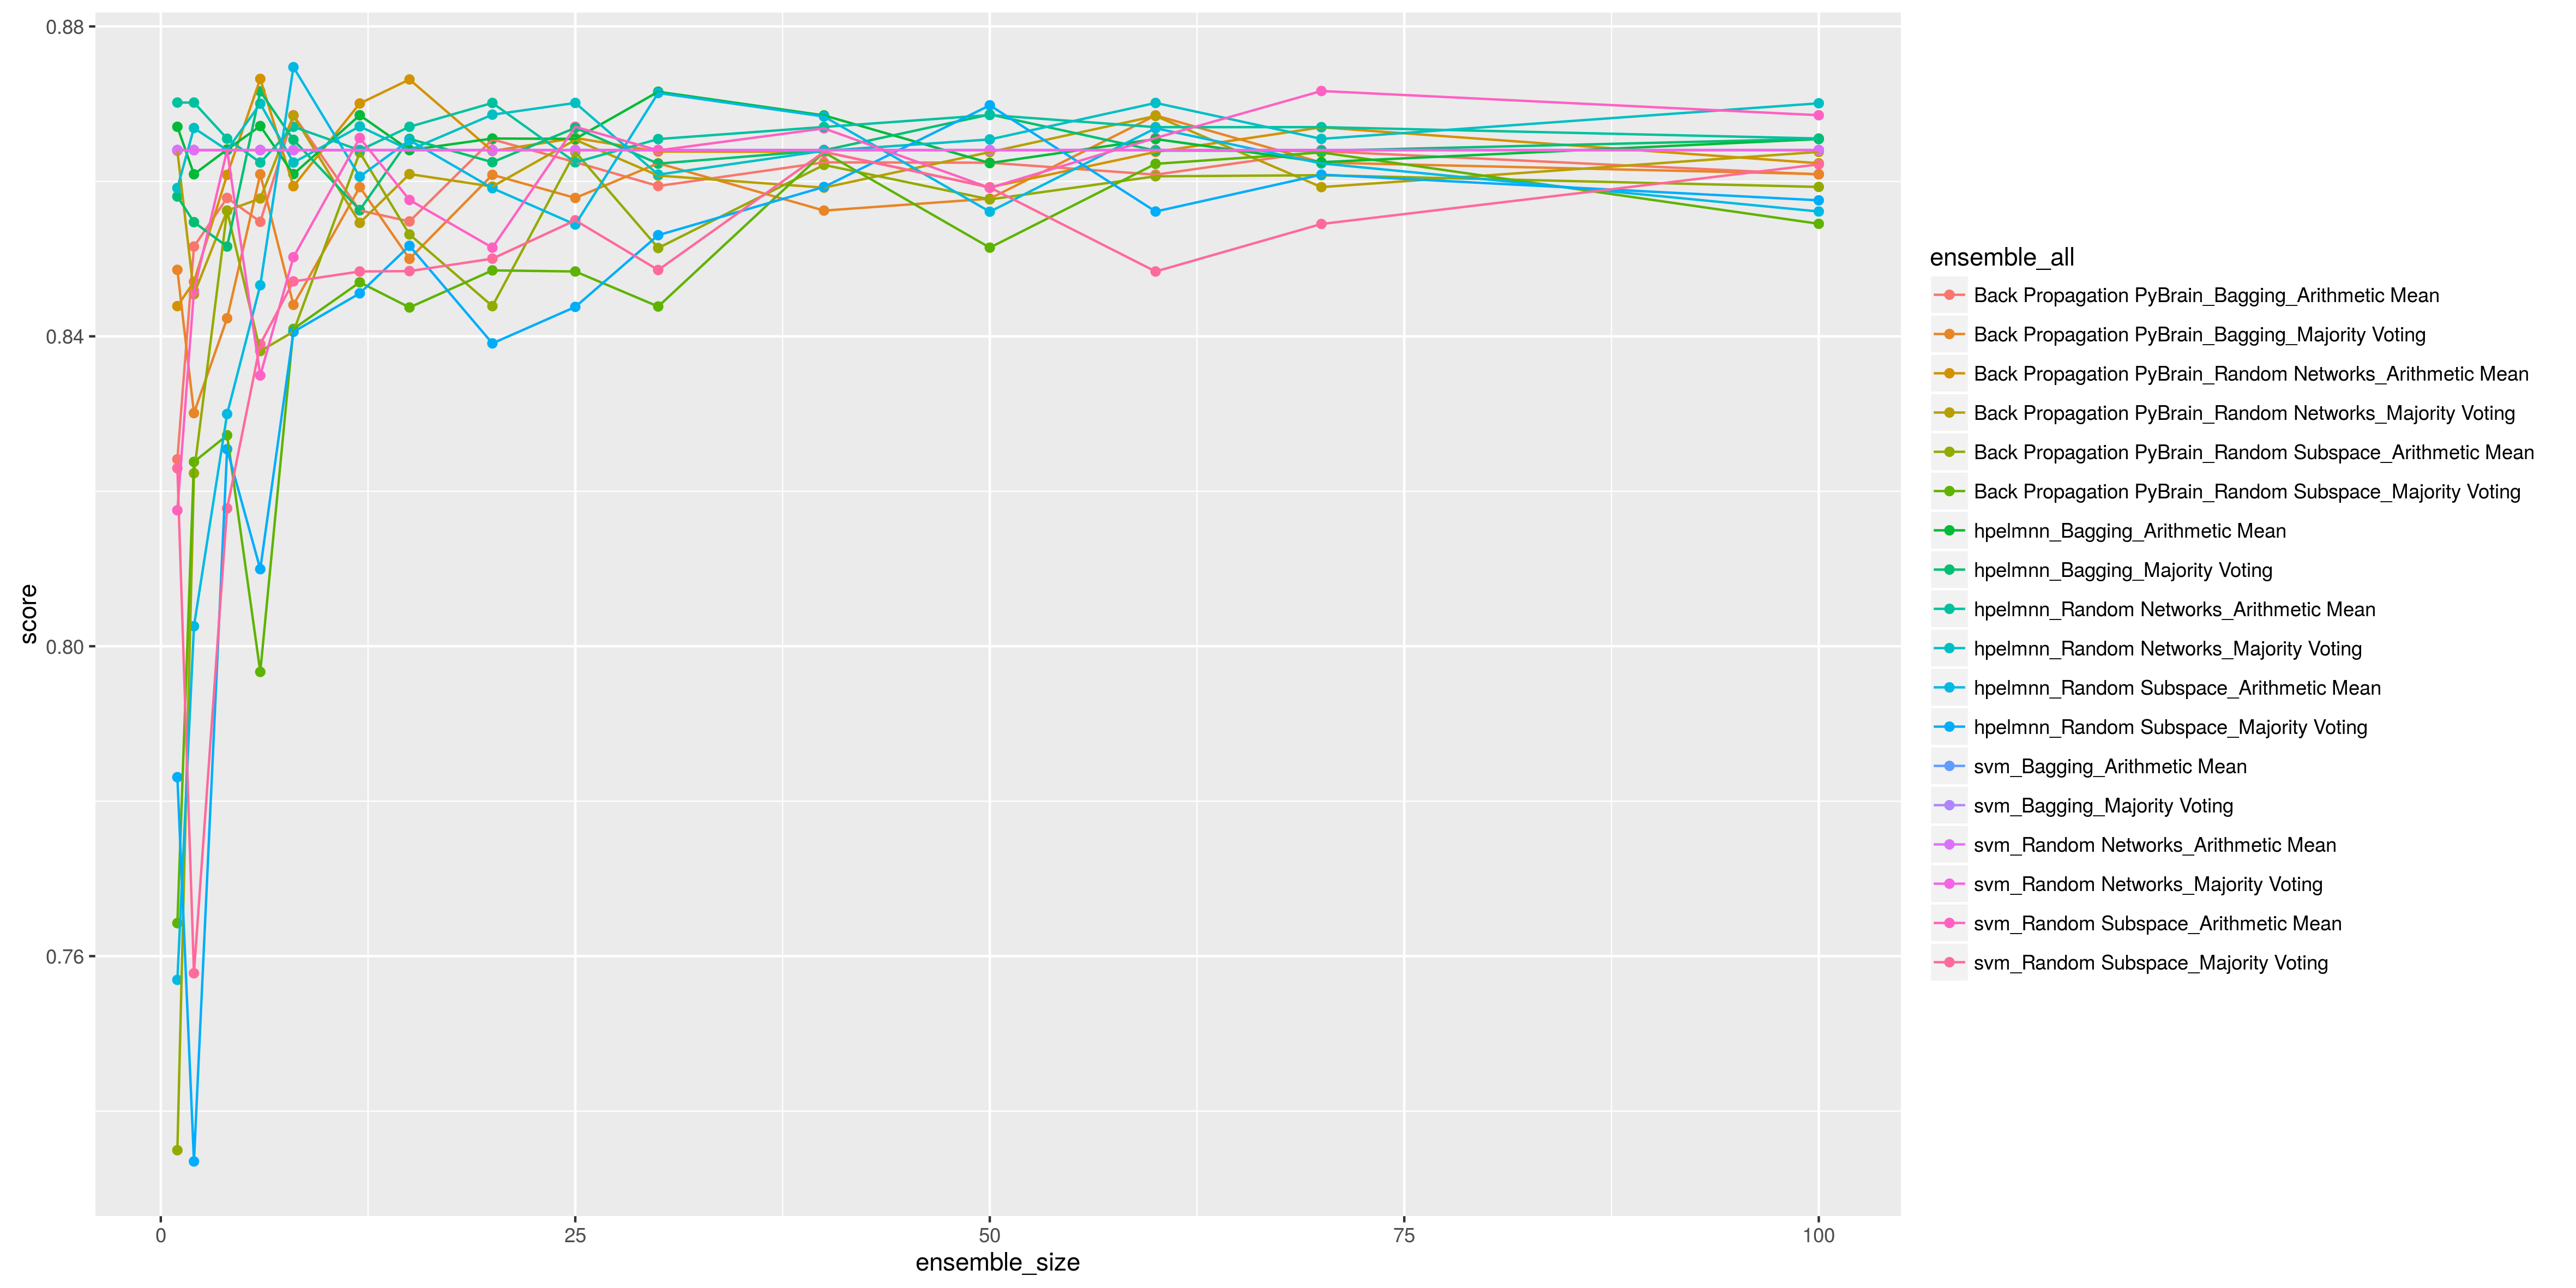
\includegraphics[width=1.0\textwidth]{type3_score_size_dataset_crx}\centering\caption{crx}\end{figure}
\begin{figure}[H]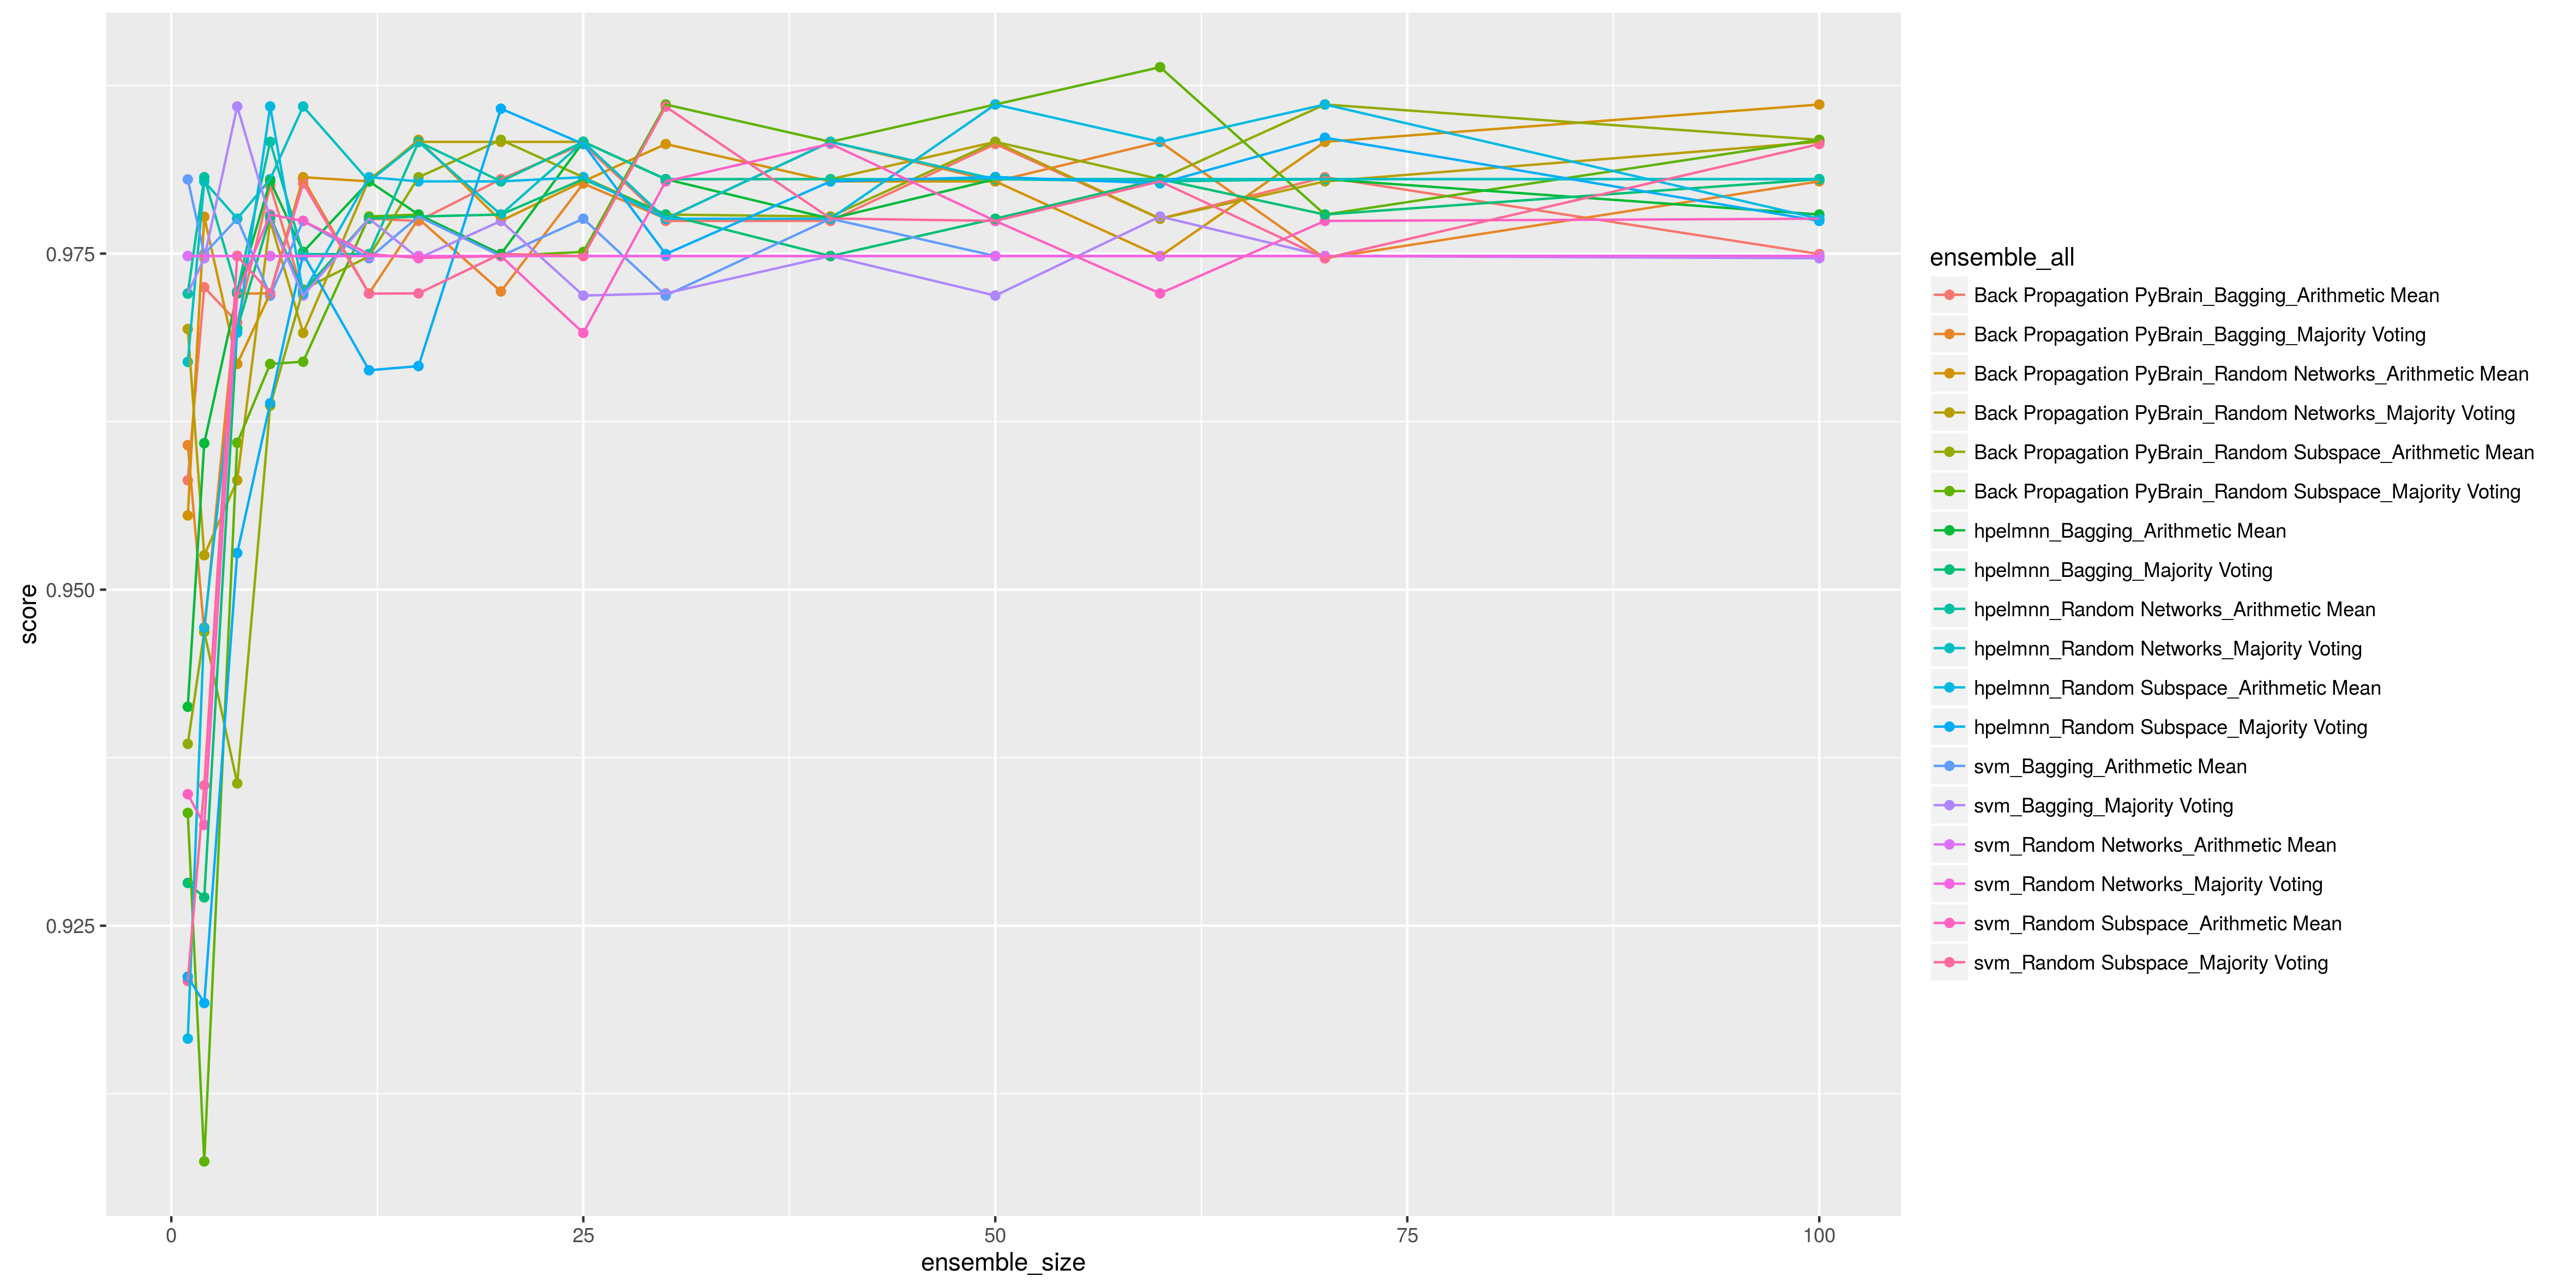
\includegraphics[width=1.0\textwidth]{type3_score_size_dataset_dermatology}\centering\caption{dermatology}\end{figure}
\begin{figure}[H]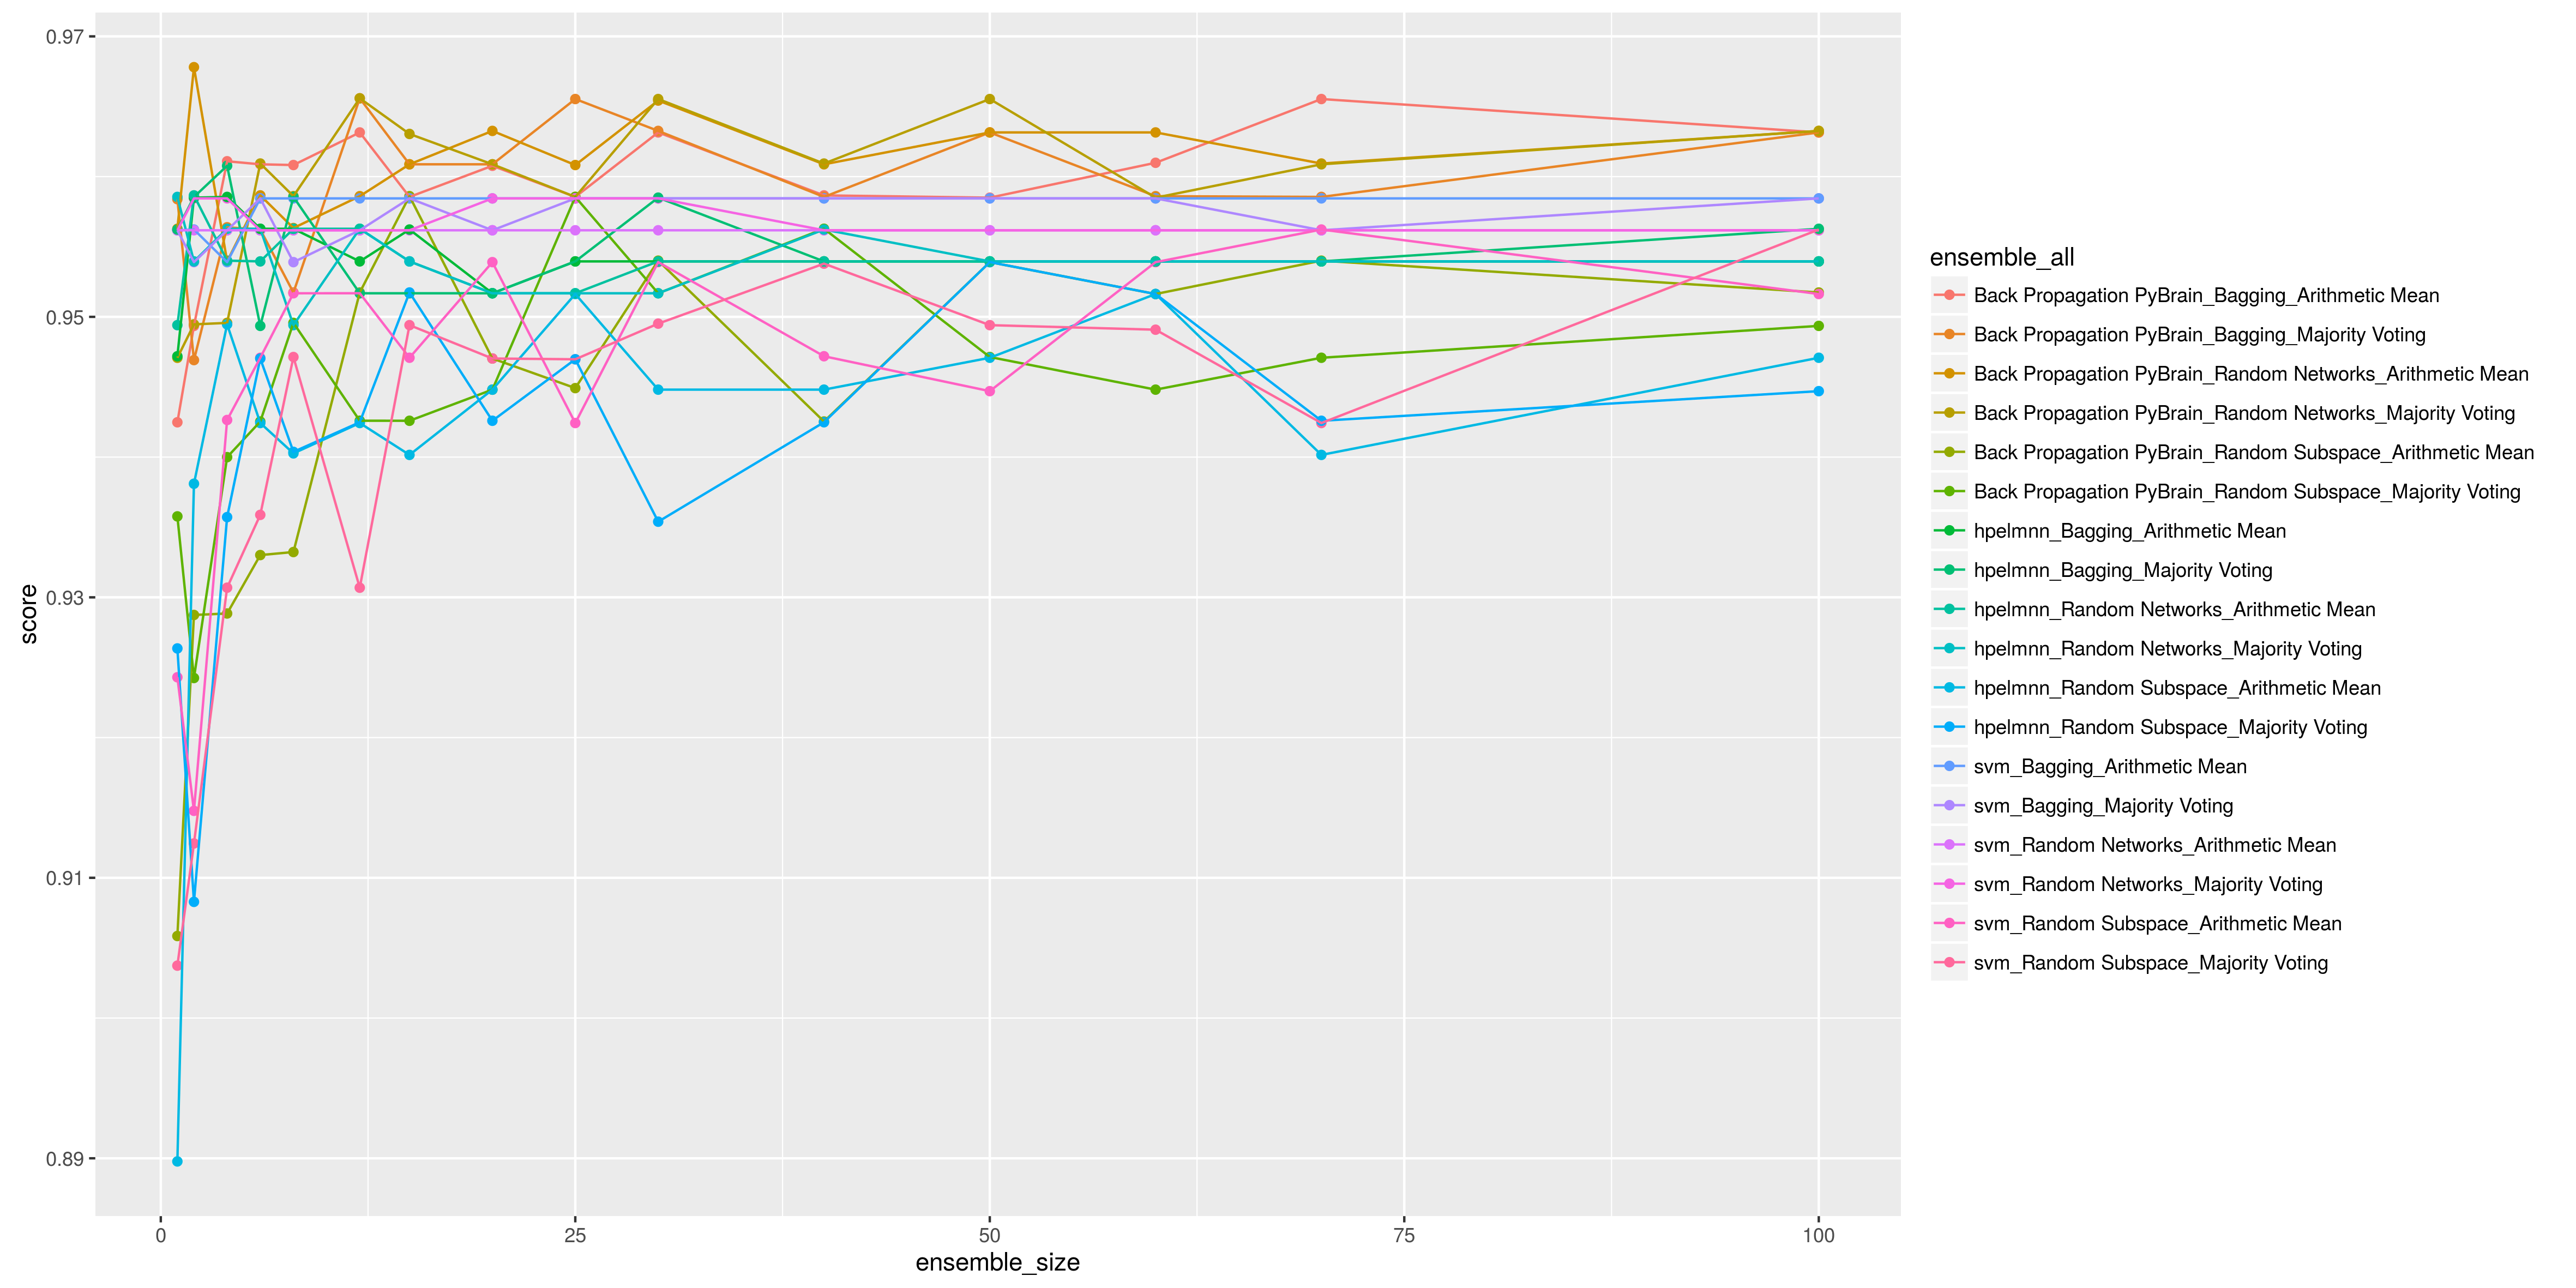
\includegraphics[width=1.0\textwidth]{type3_score_size_dataset_house_votes}\centering\caption{house\_votes}\end{figure}
\begin{figure}[H]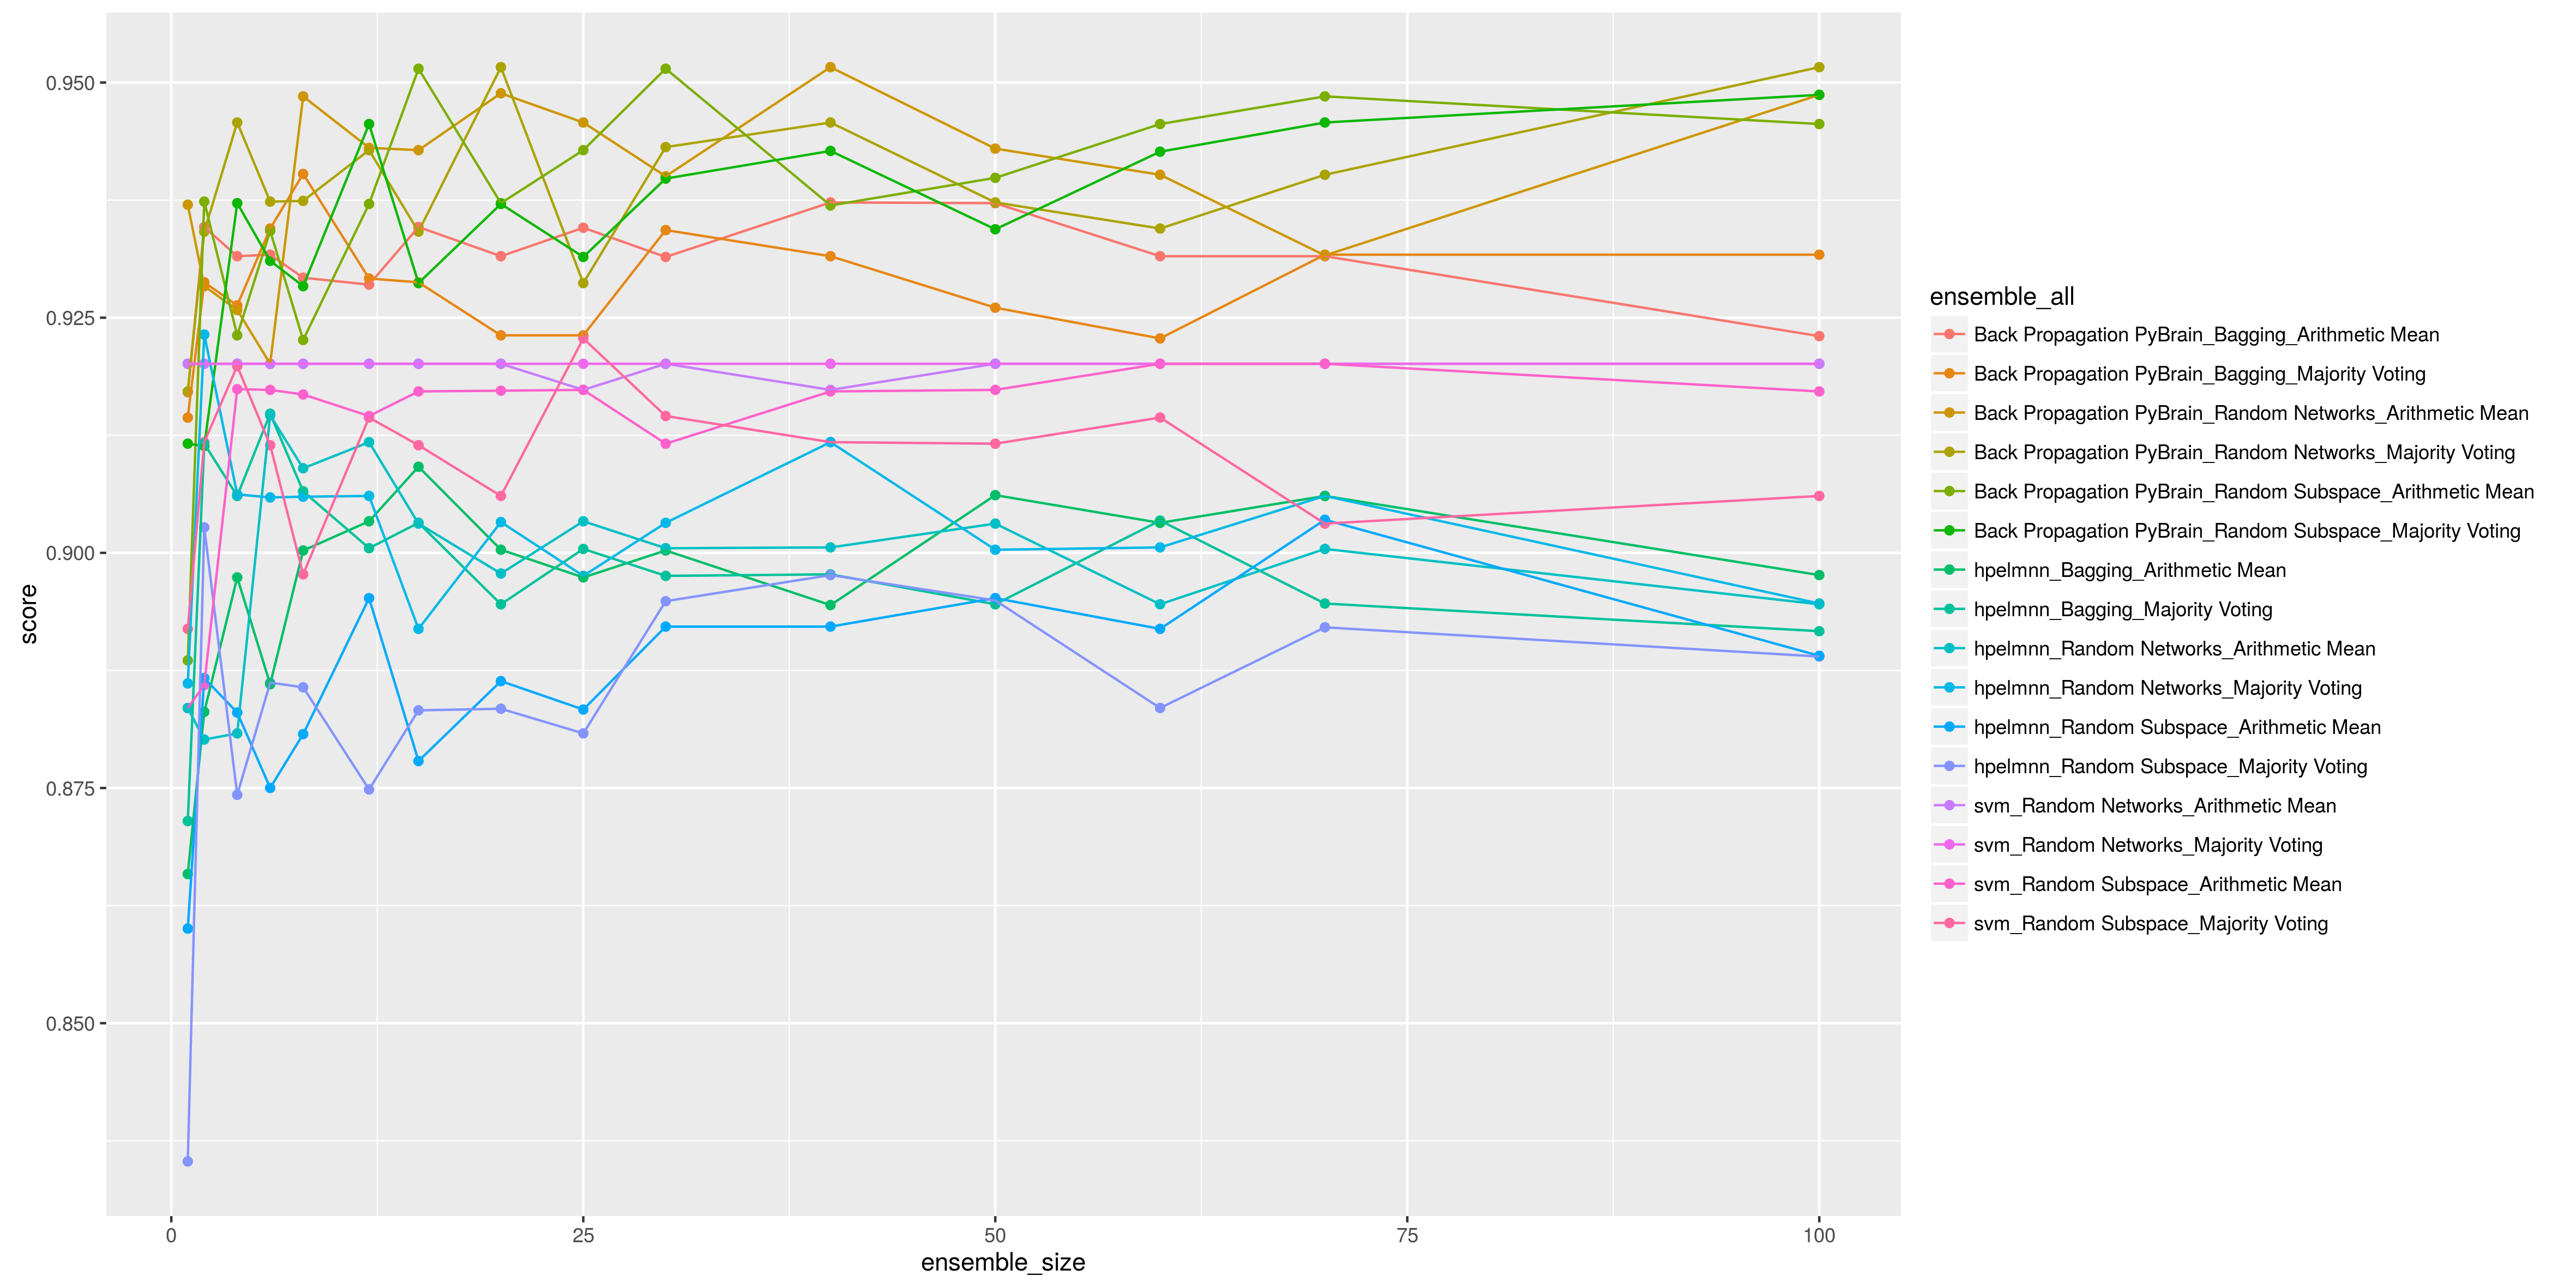
\includegraphics[width=1.0\textwidth]{type3_score_size_dataset_ionosphere}\centering\caption{ionosphere}\end{figure}
\begin{figure}[H]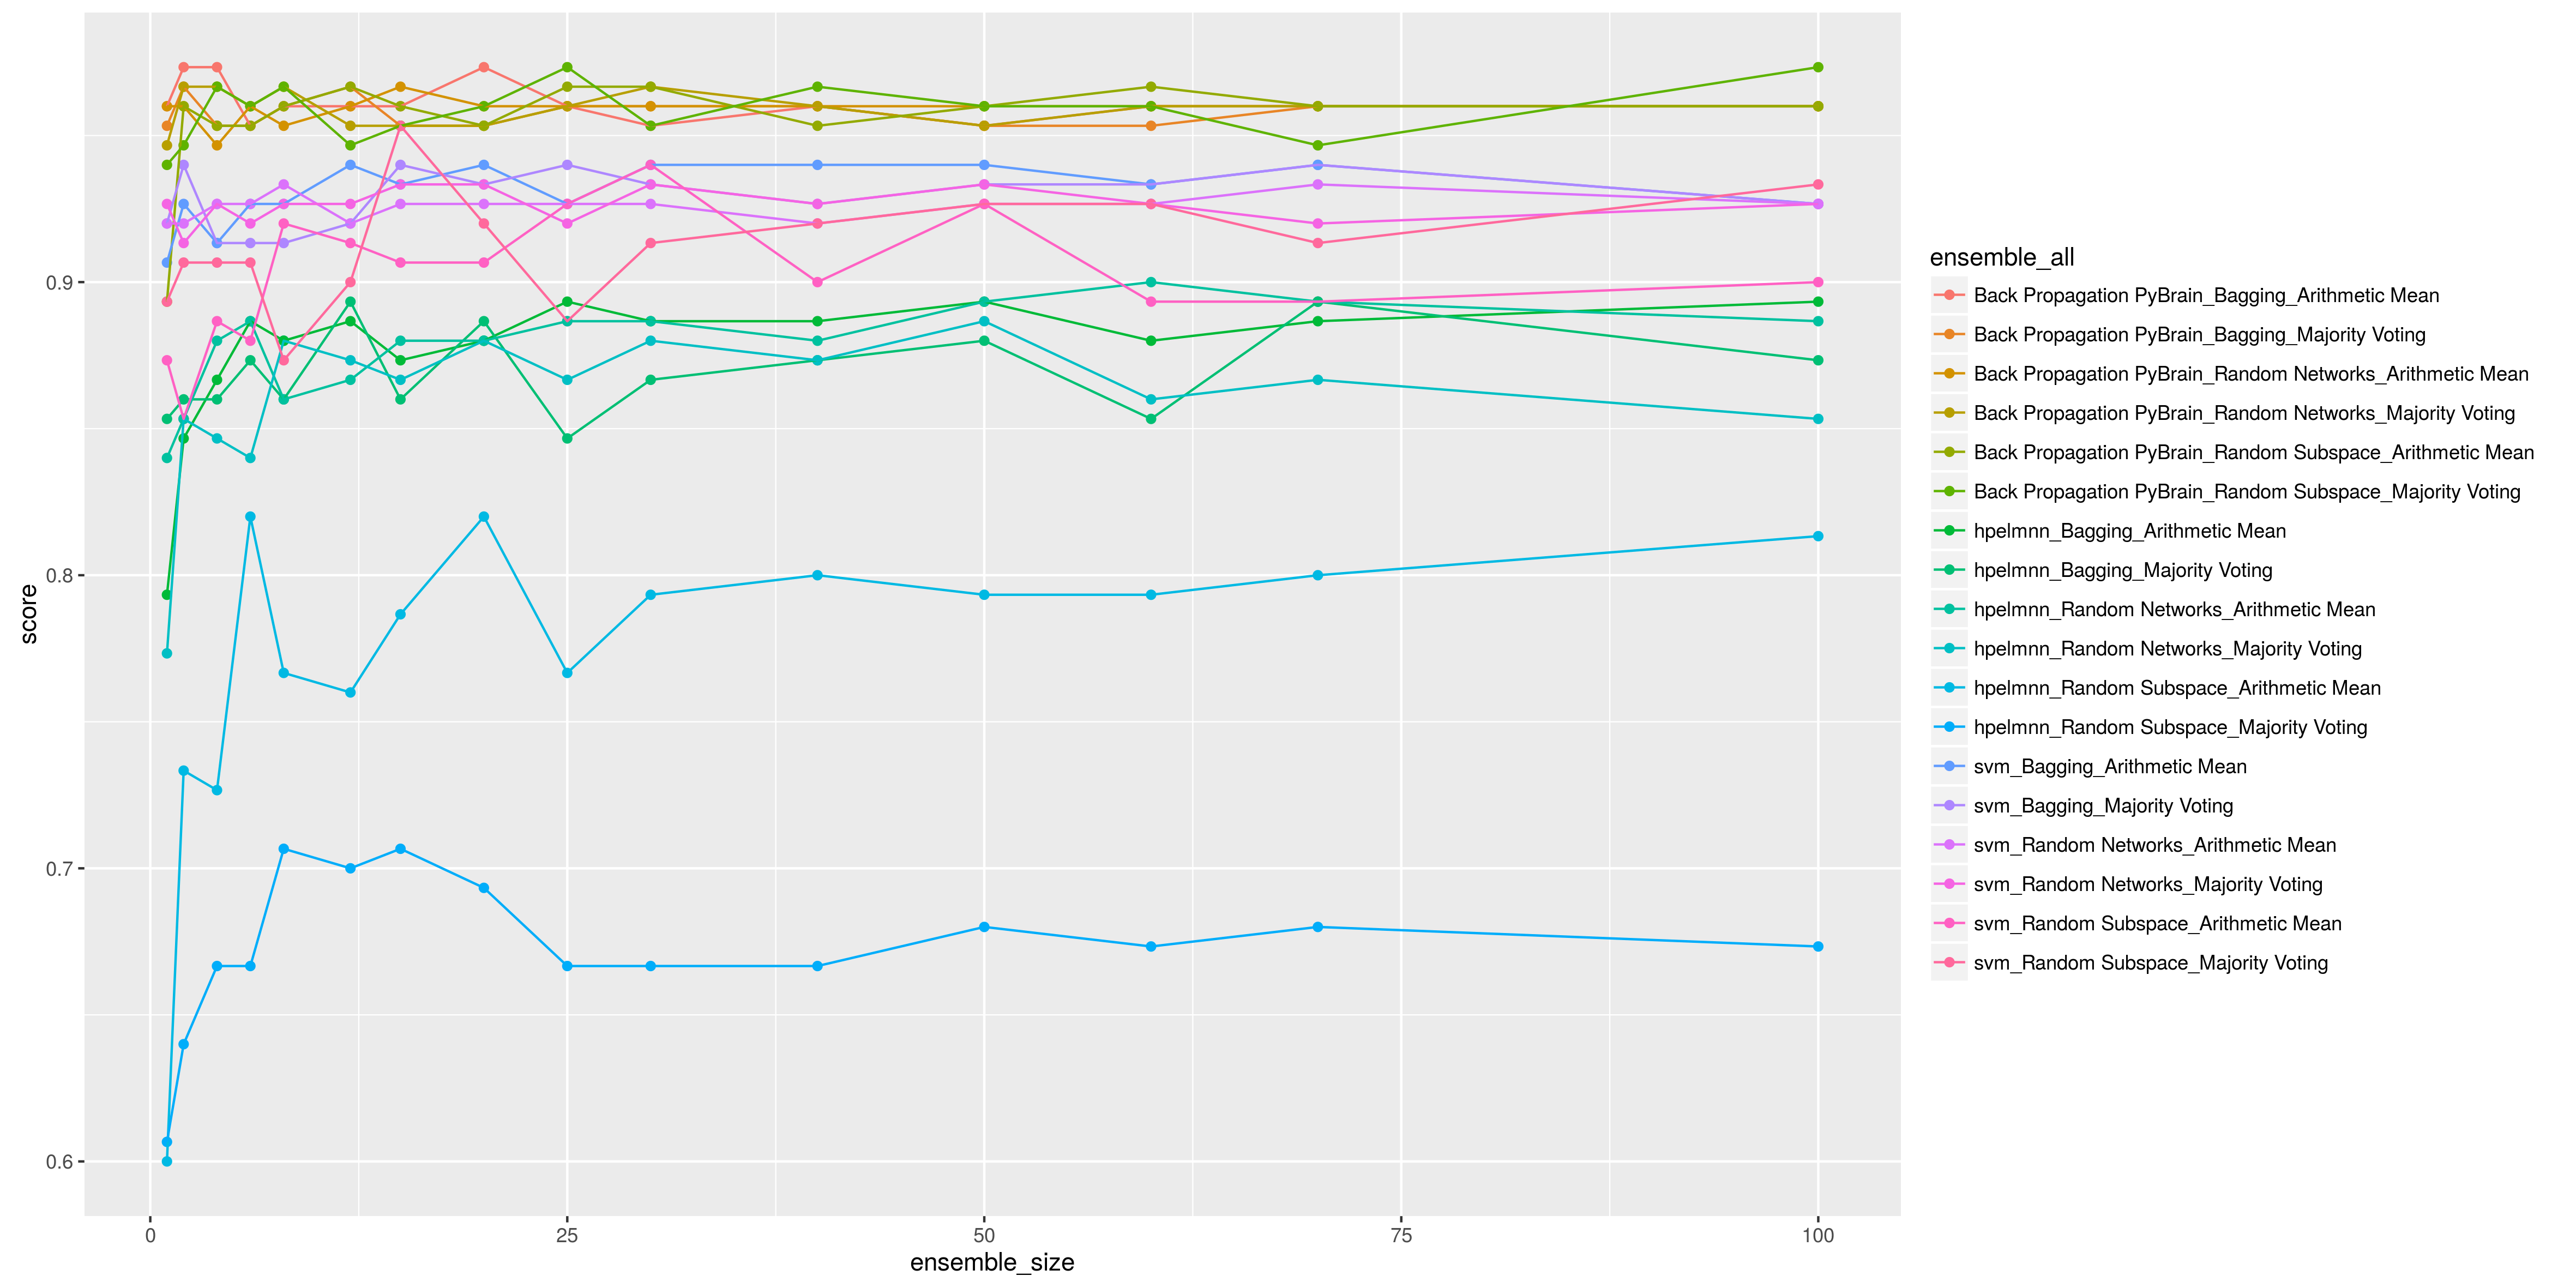
\includegraphics[width=1.0\textwidth]{type3_score_size_dataset_iris}\centering\caption{iris}\end{figure}
\begin{figure}[H]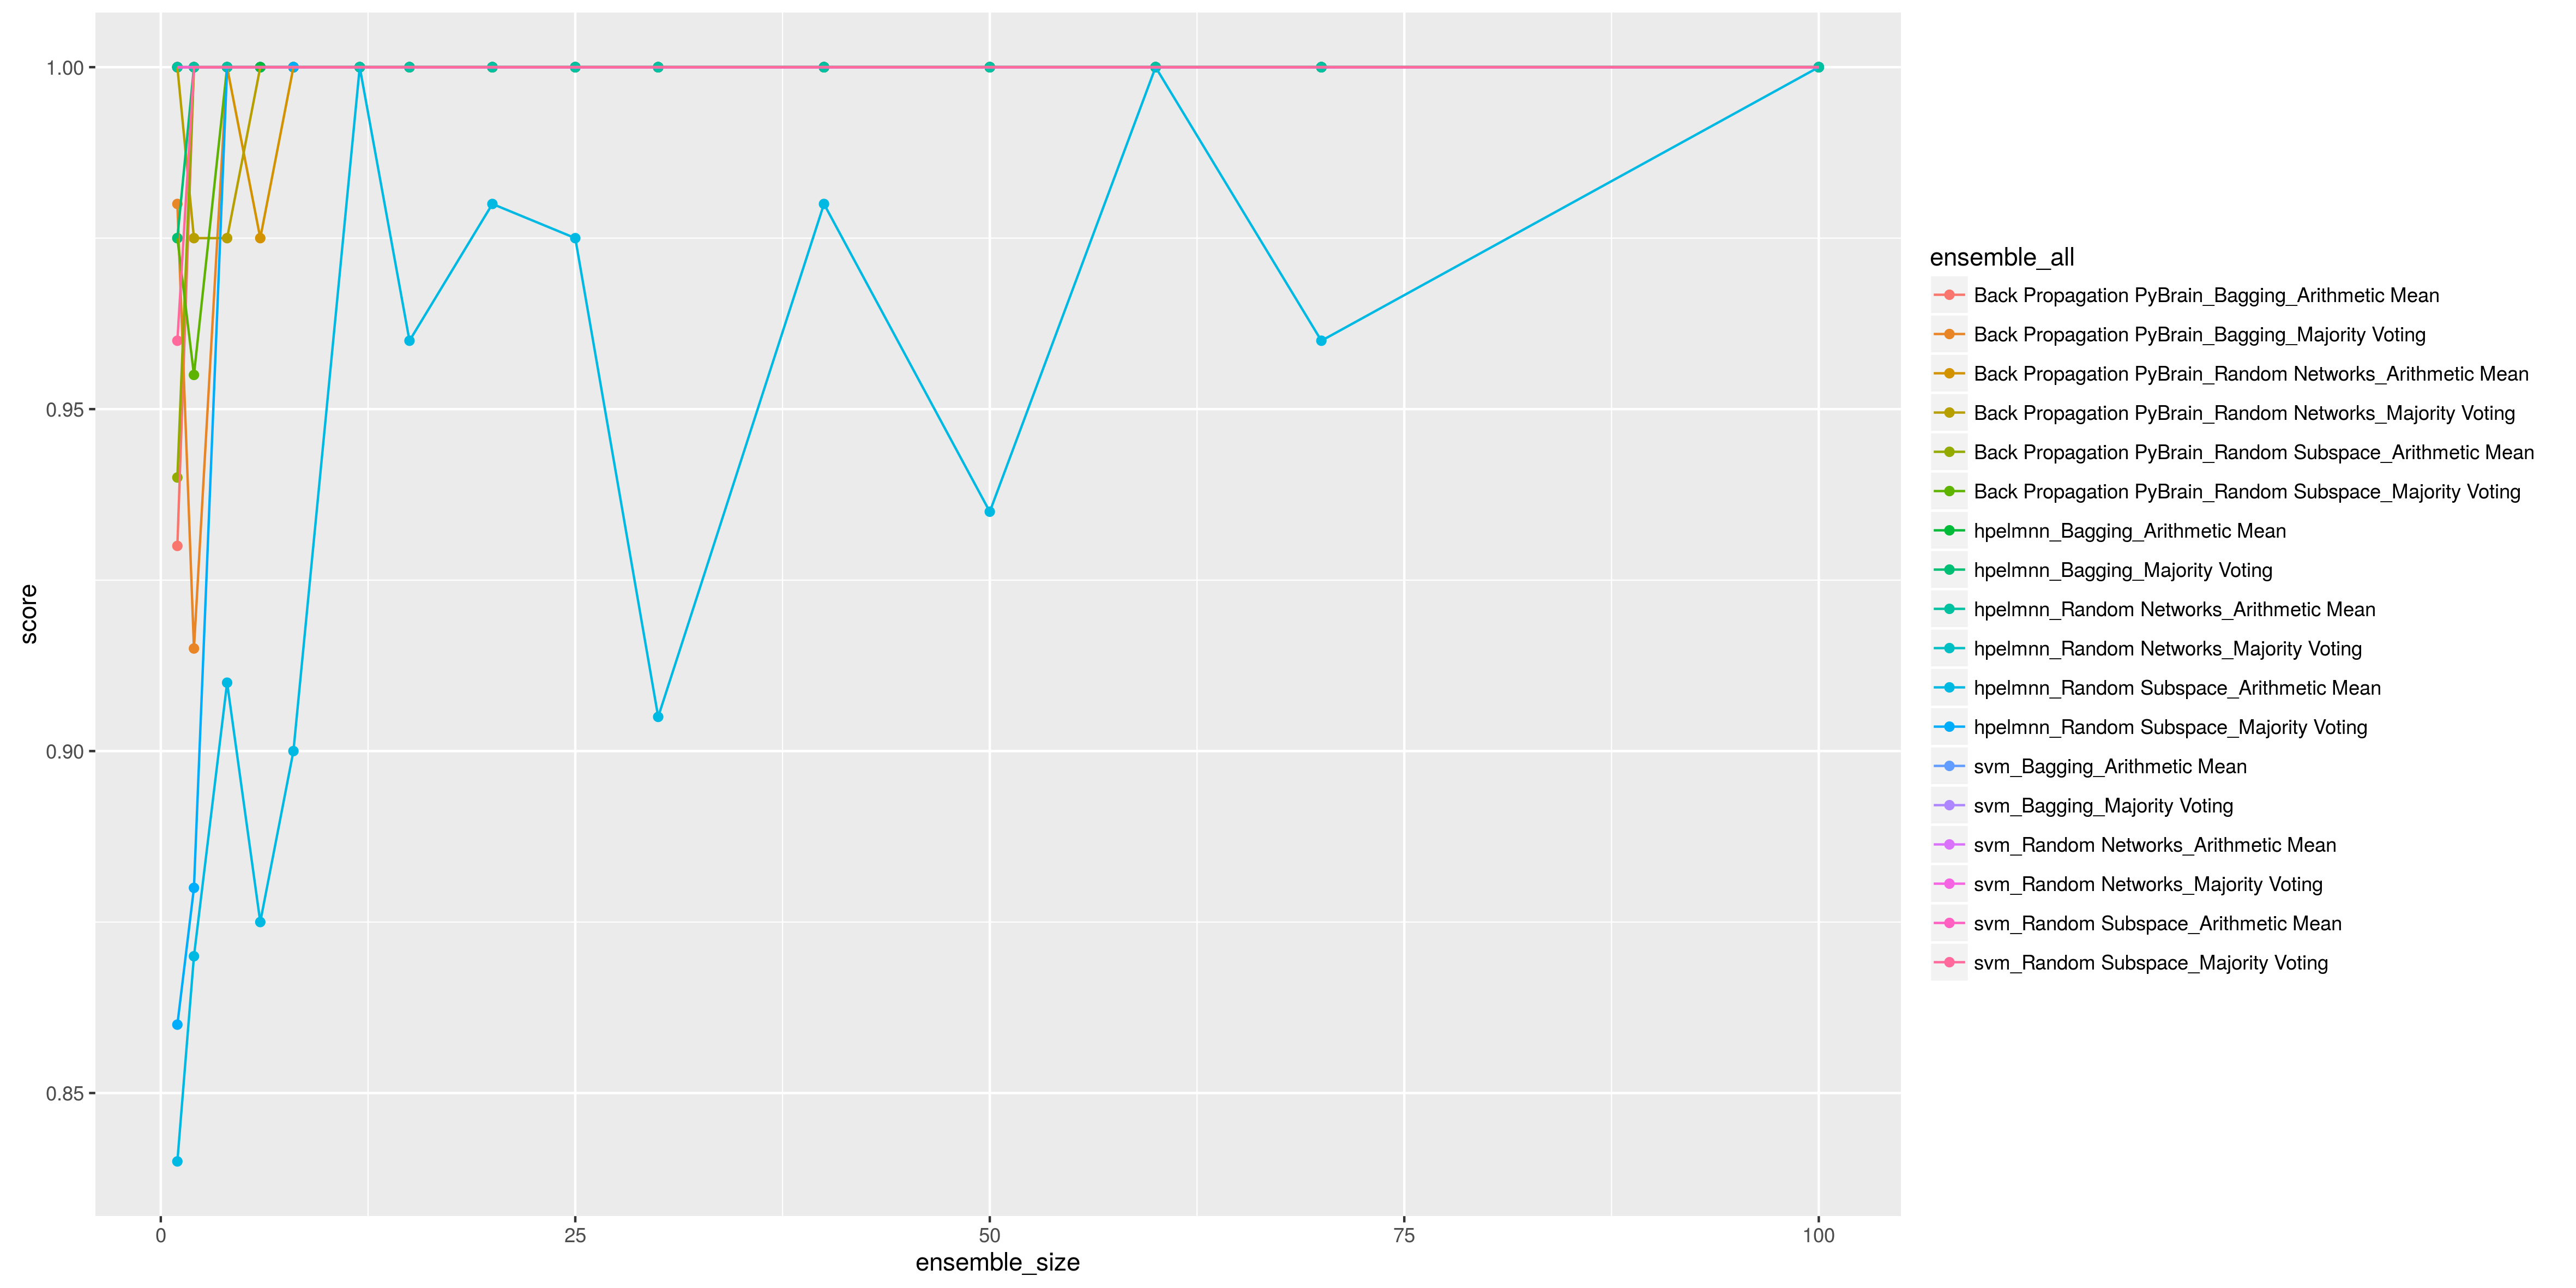
\includegraphics[width=1.0\textwidth]{type3_score_size_dataset_soybean_small}\centering\caption{soybean\_small}\end{figure}
\begin{figure}[H]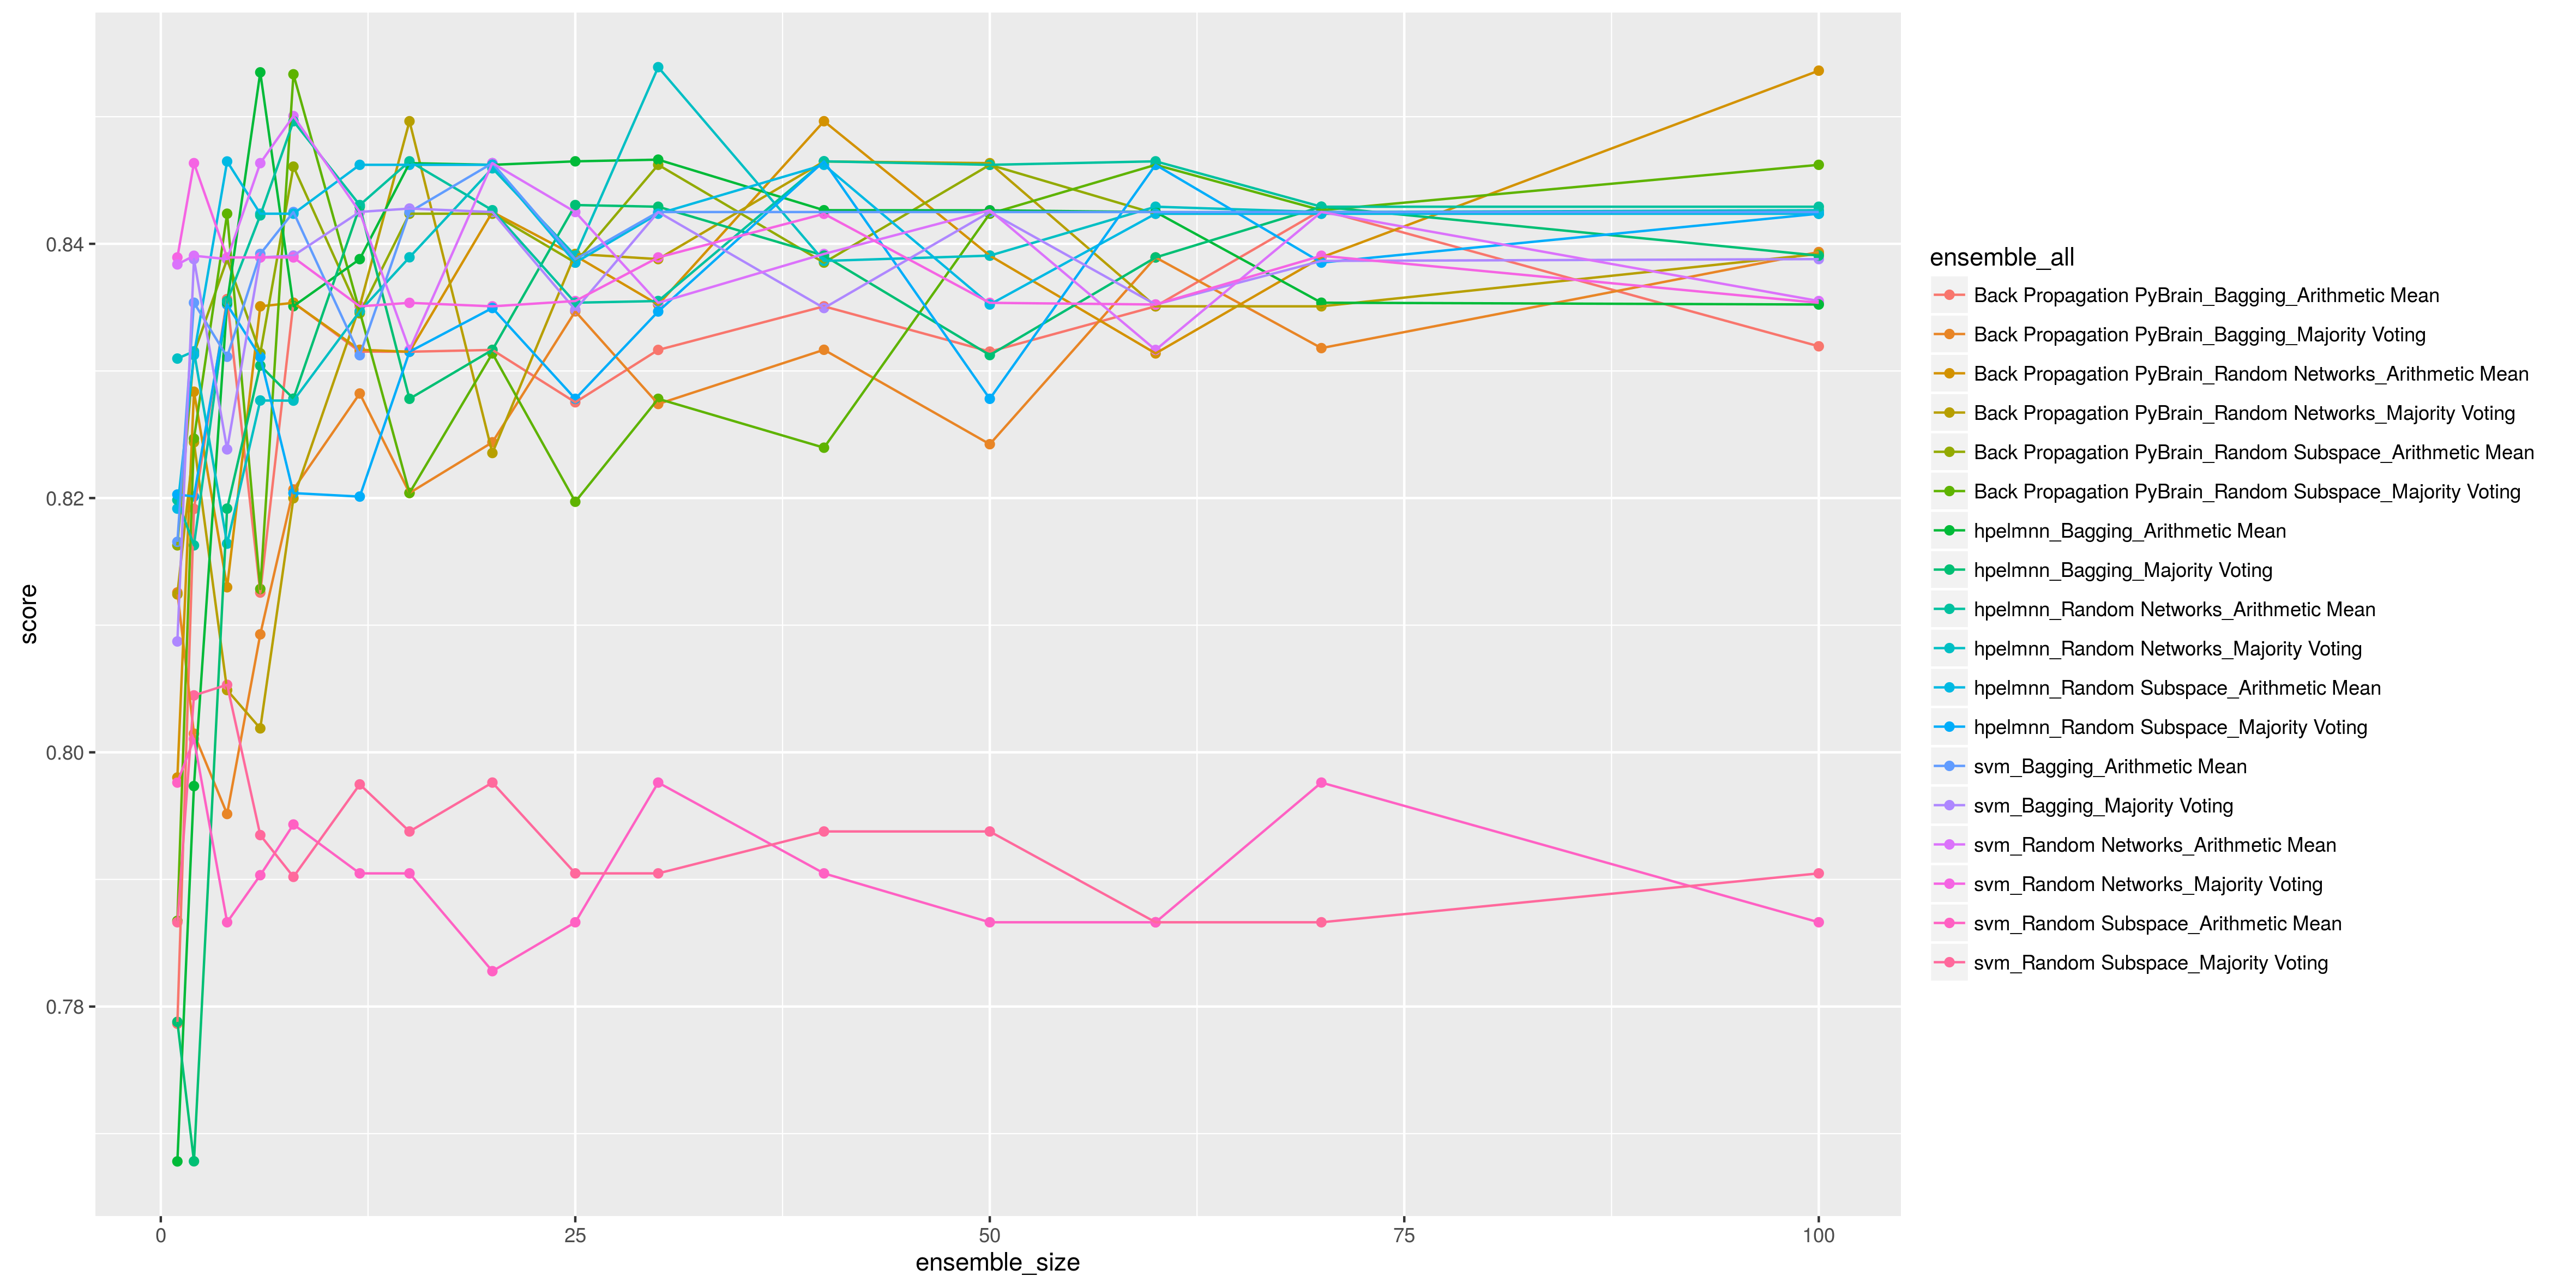
\includegraphics[width=1.0\textwidth]{type3_score_size_dataset_spect}\centering\caption{spect}\end{figure}
\begin{figure}[H]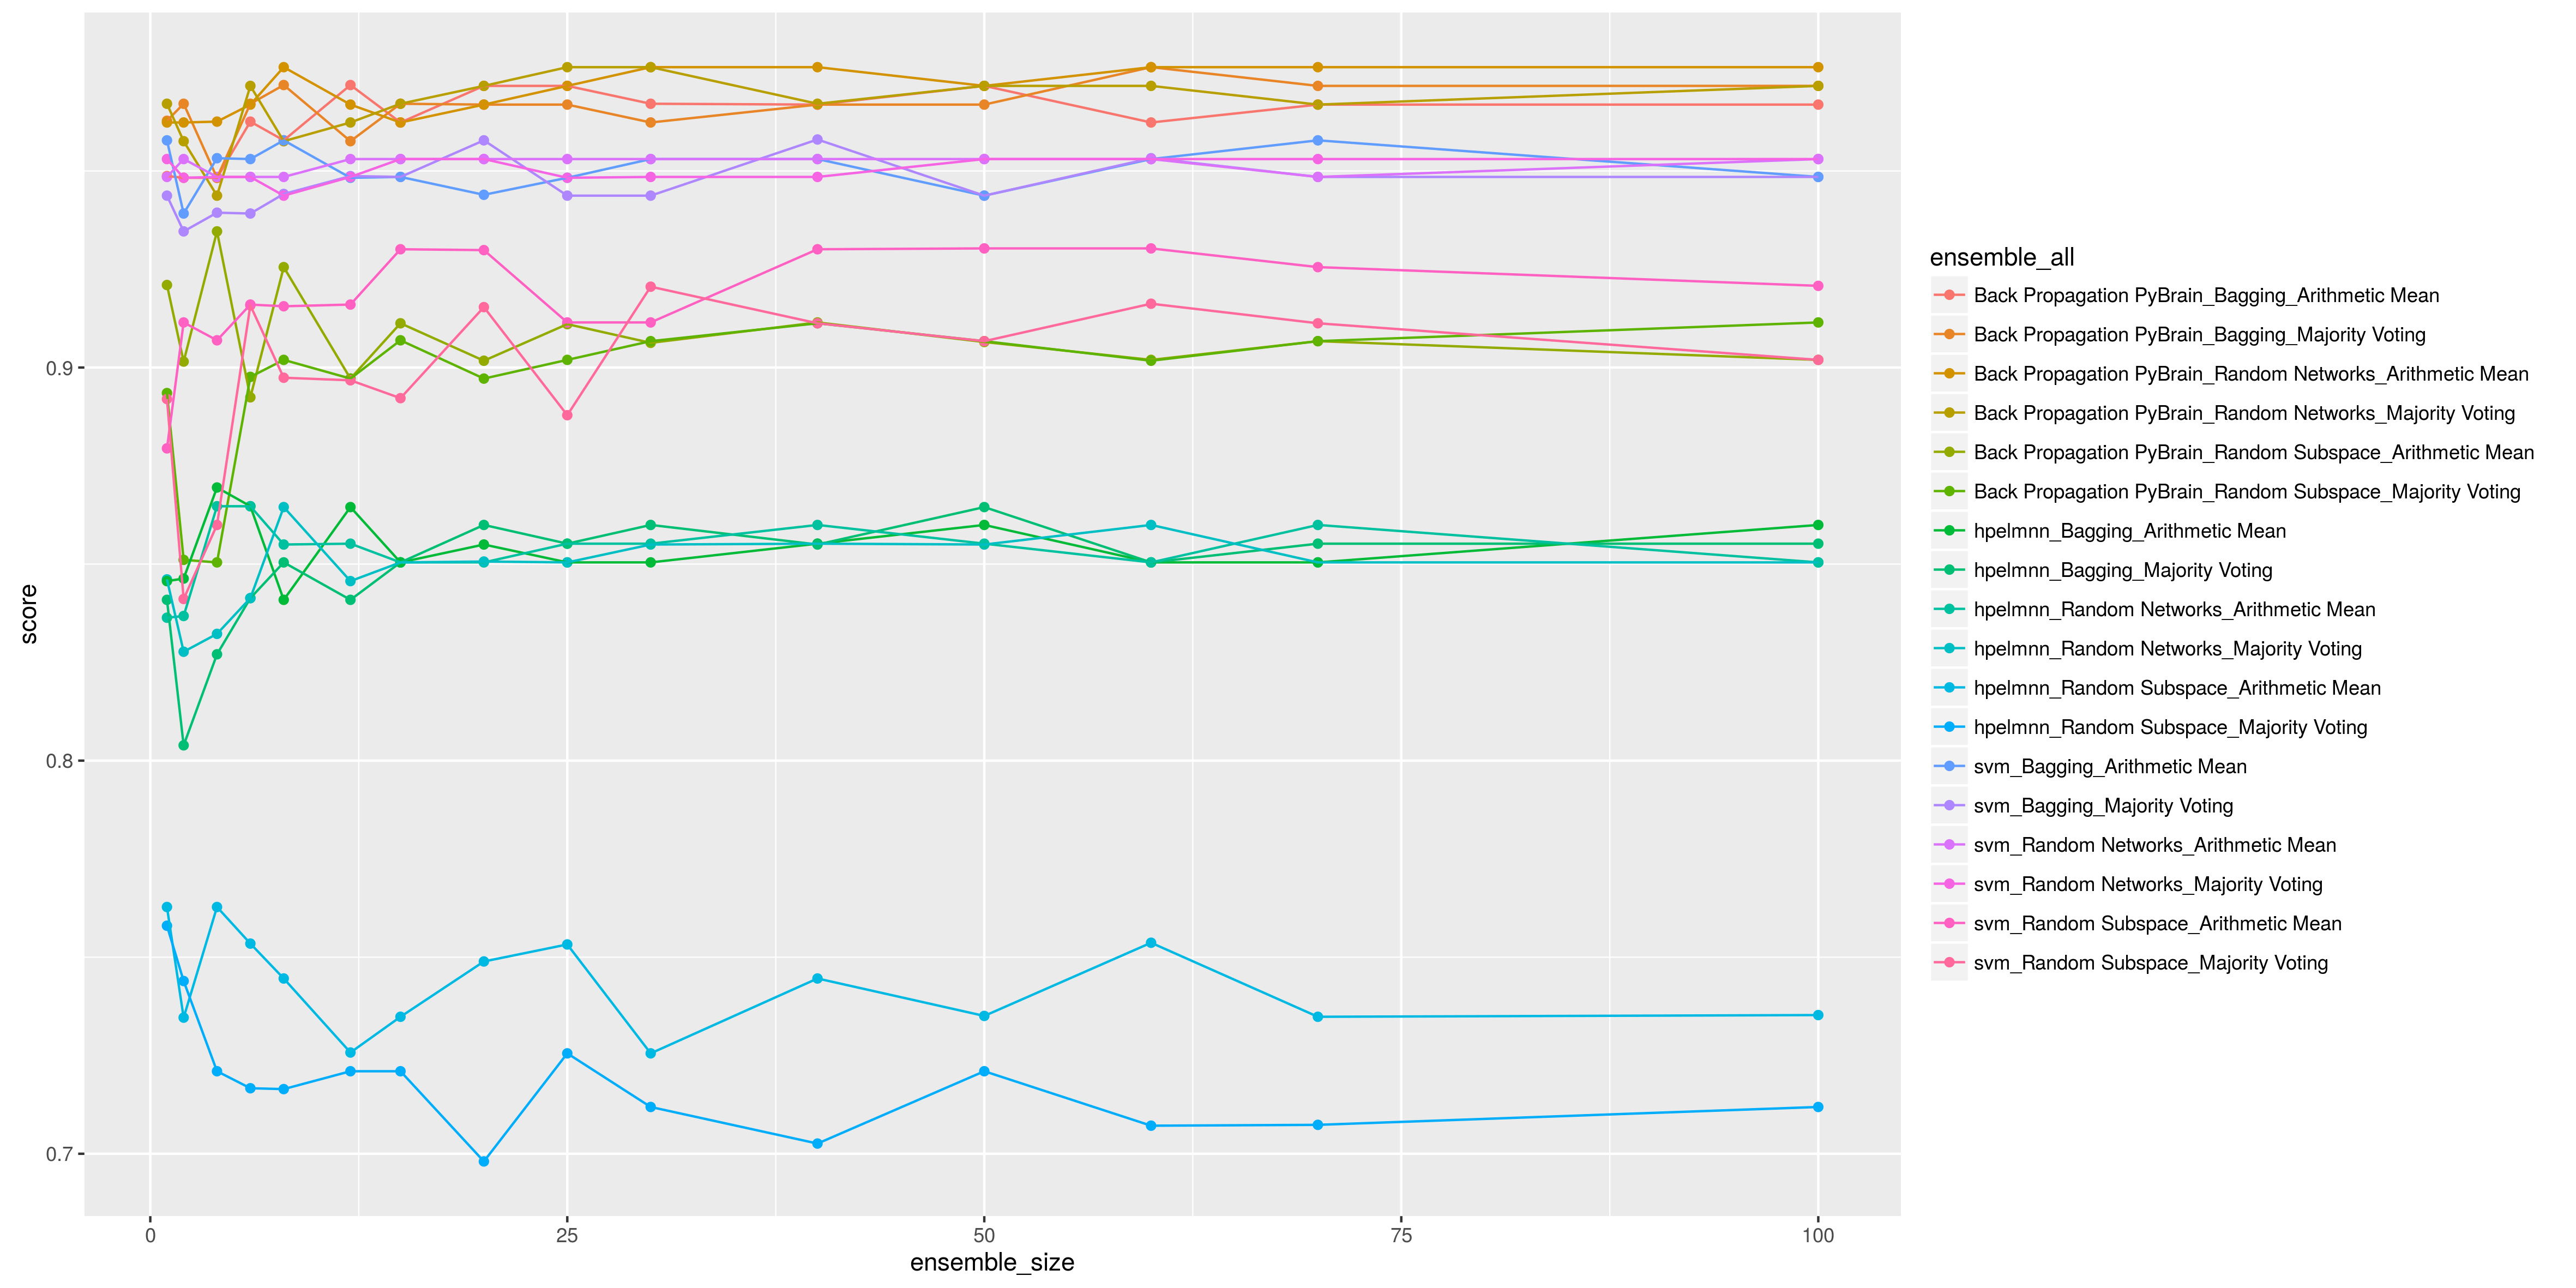
\includegraphics[width=1.0\textwidth]{type3_score_size_dataset_thyroid}\centering\caption{thyroid}\end{figure}
\begin{figure}[H]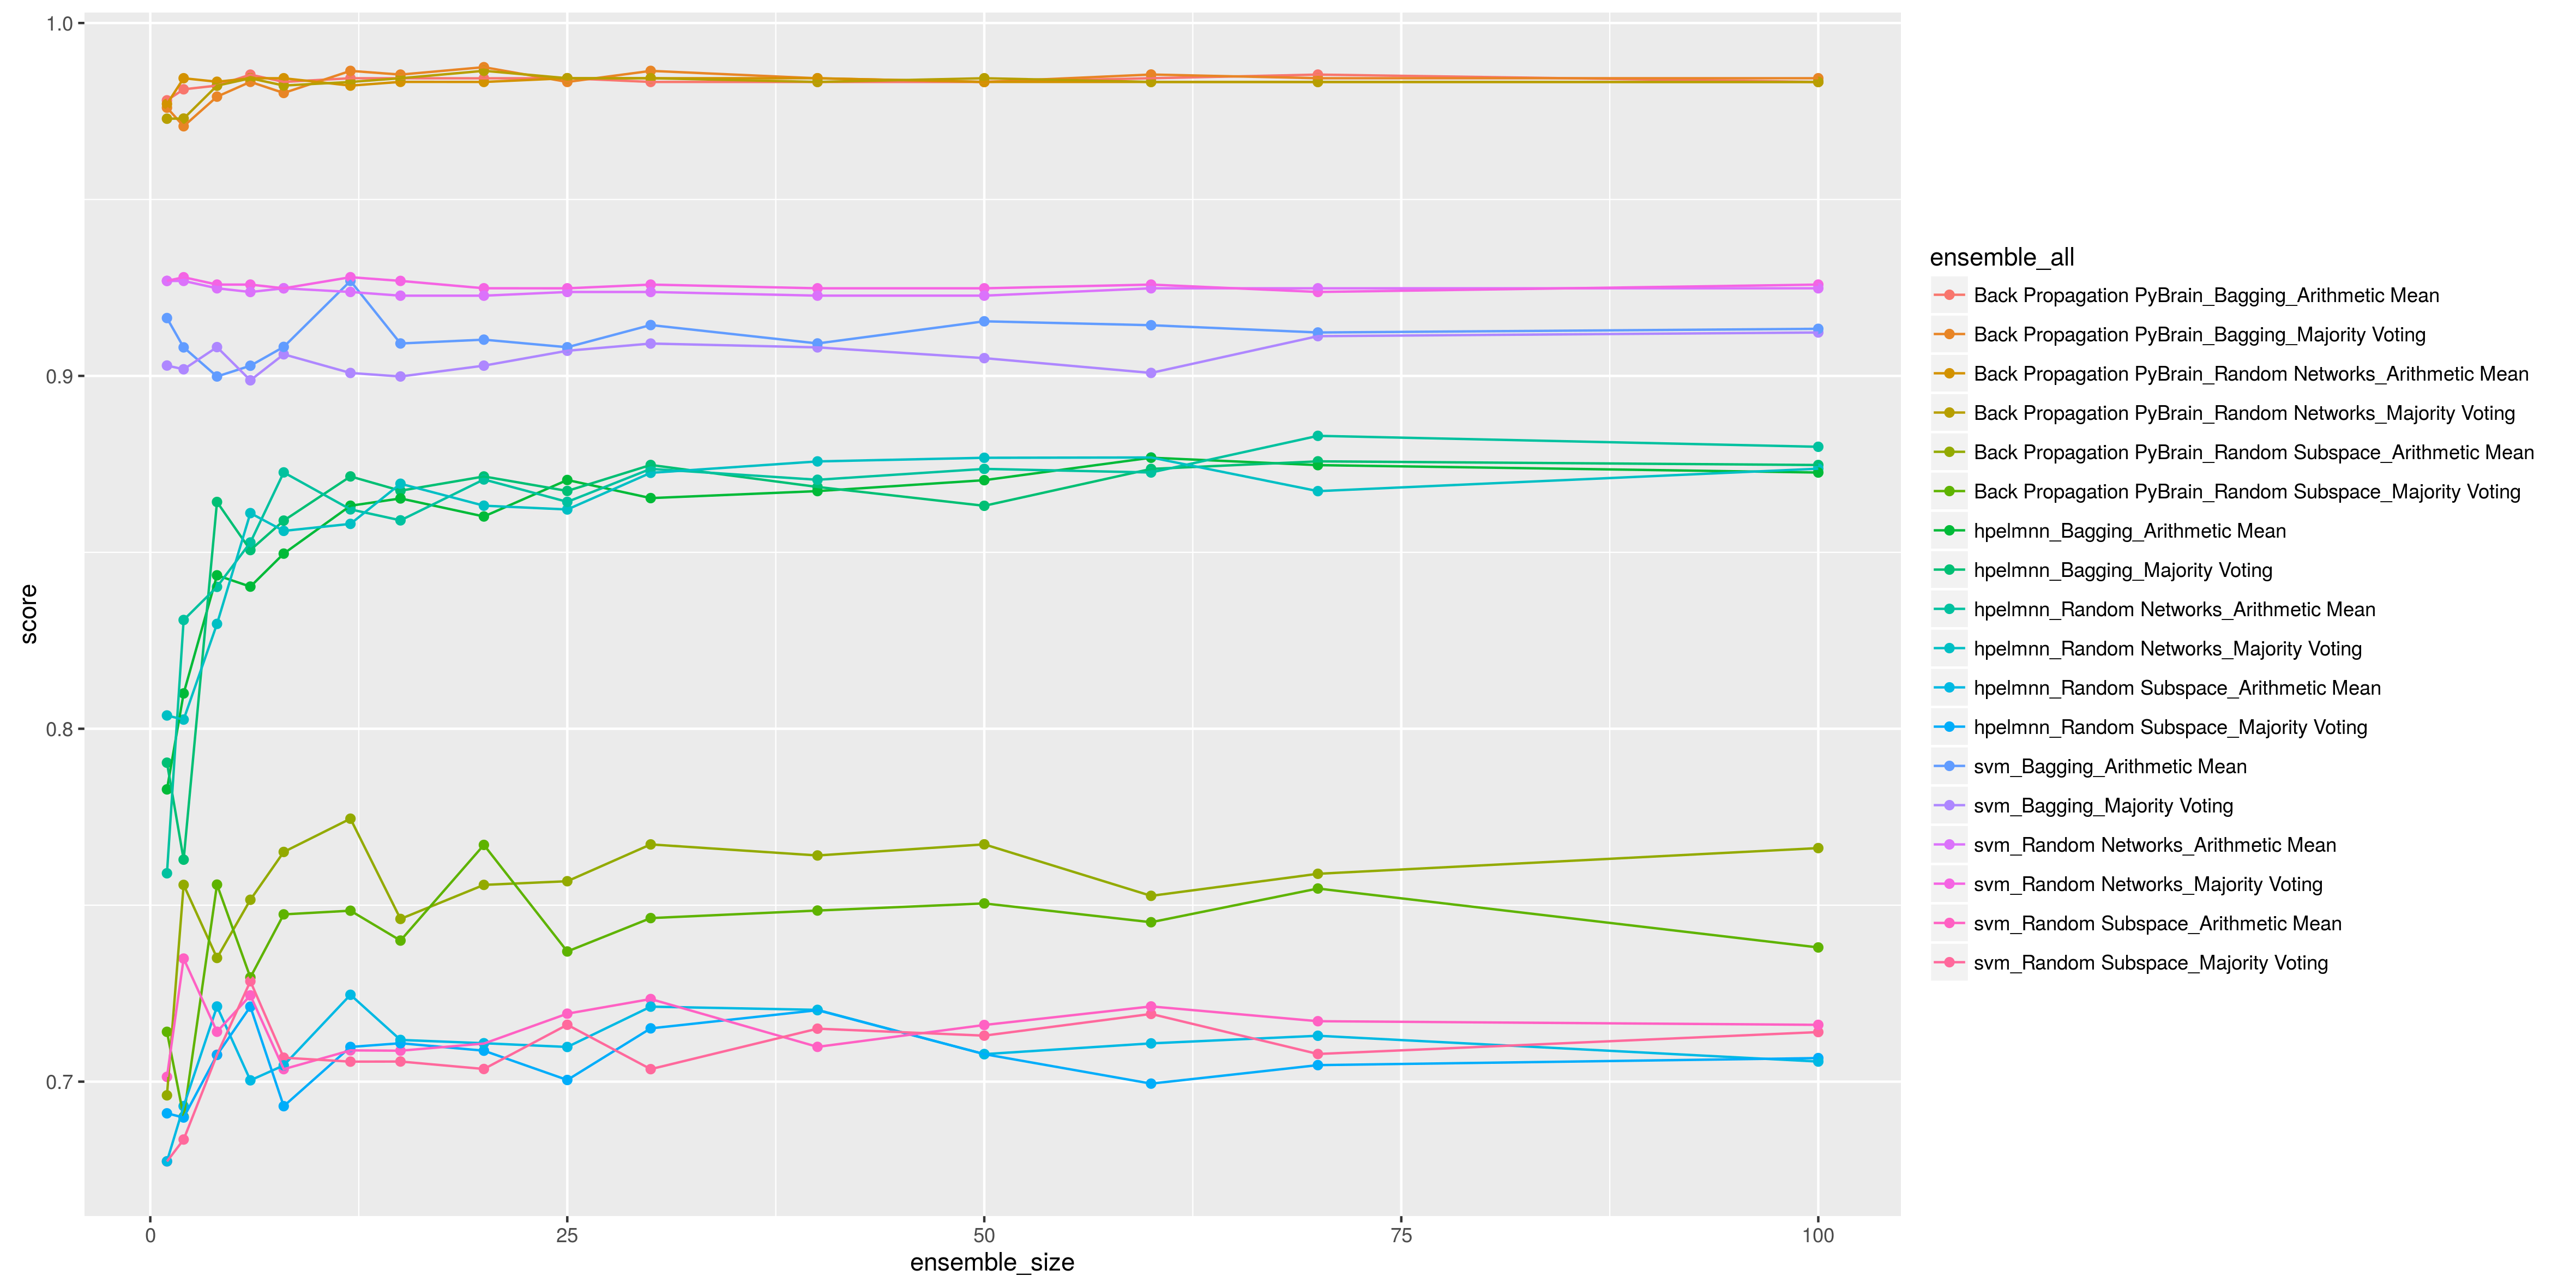
\includegraphics[width=1.0\textwidth]{type3_score_size_dataset_tic_tac_toe}\centering\caption{tic\_tac\_toe}\end{figure}
\begin{figure}[H]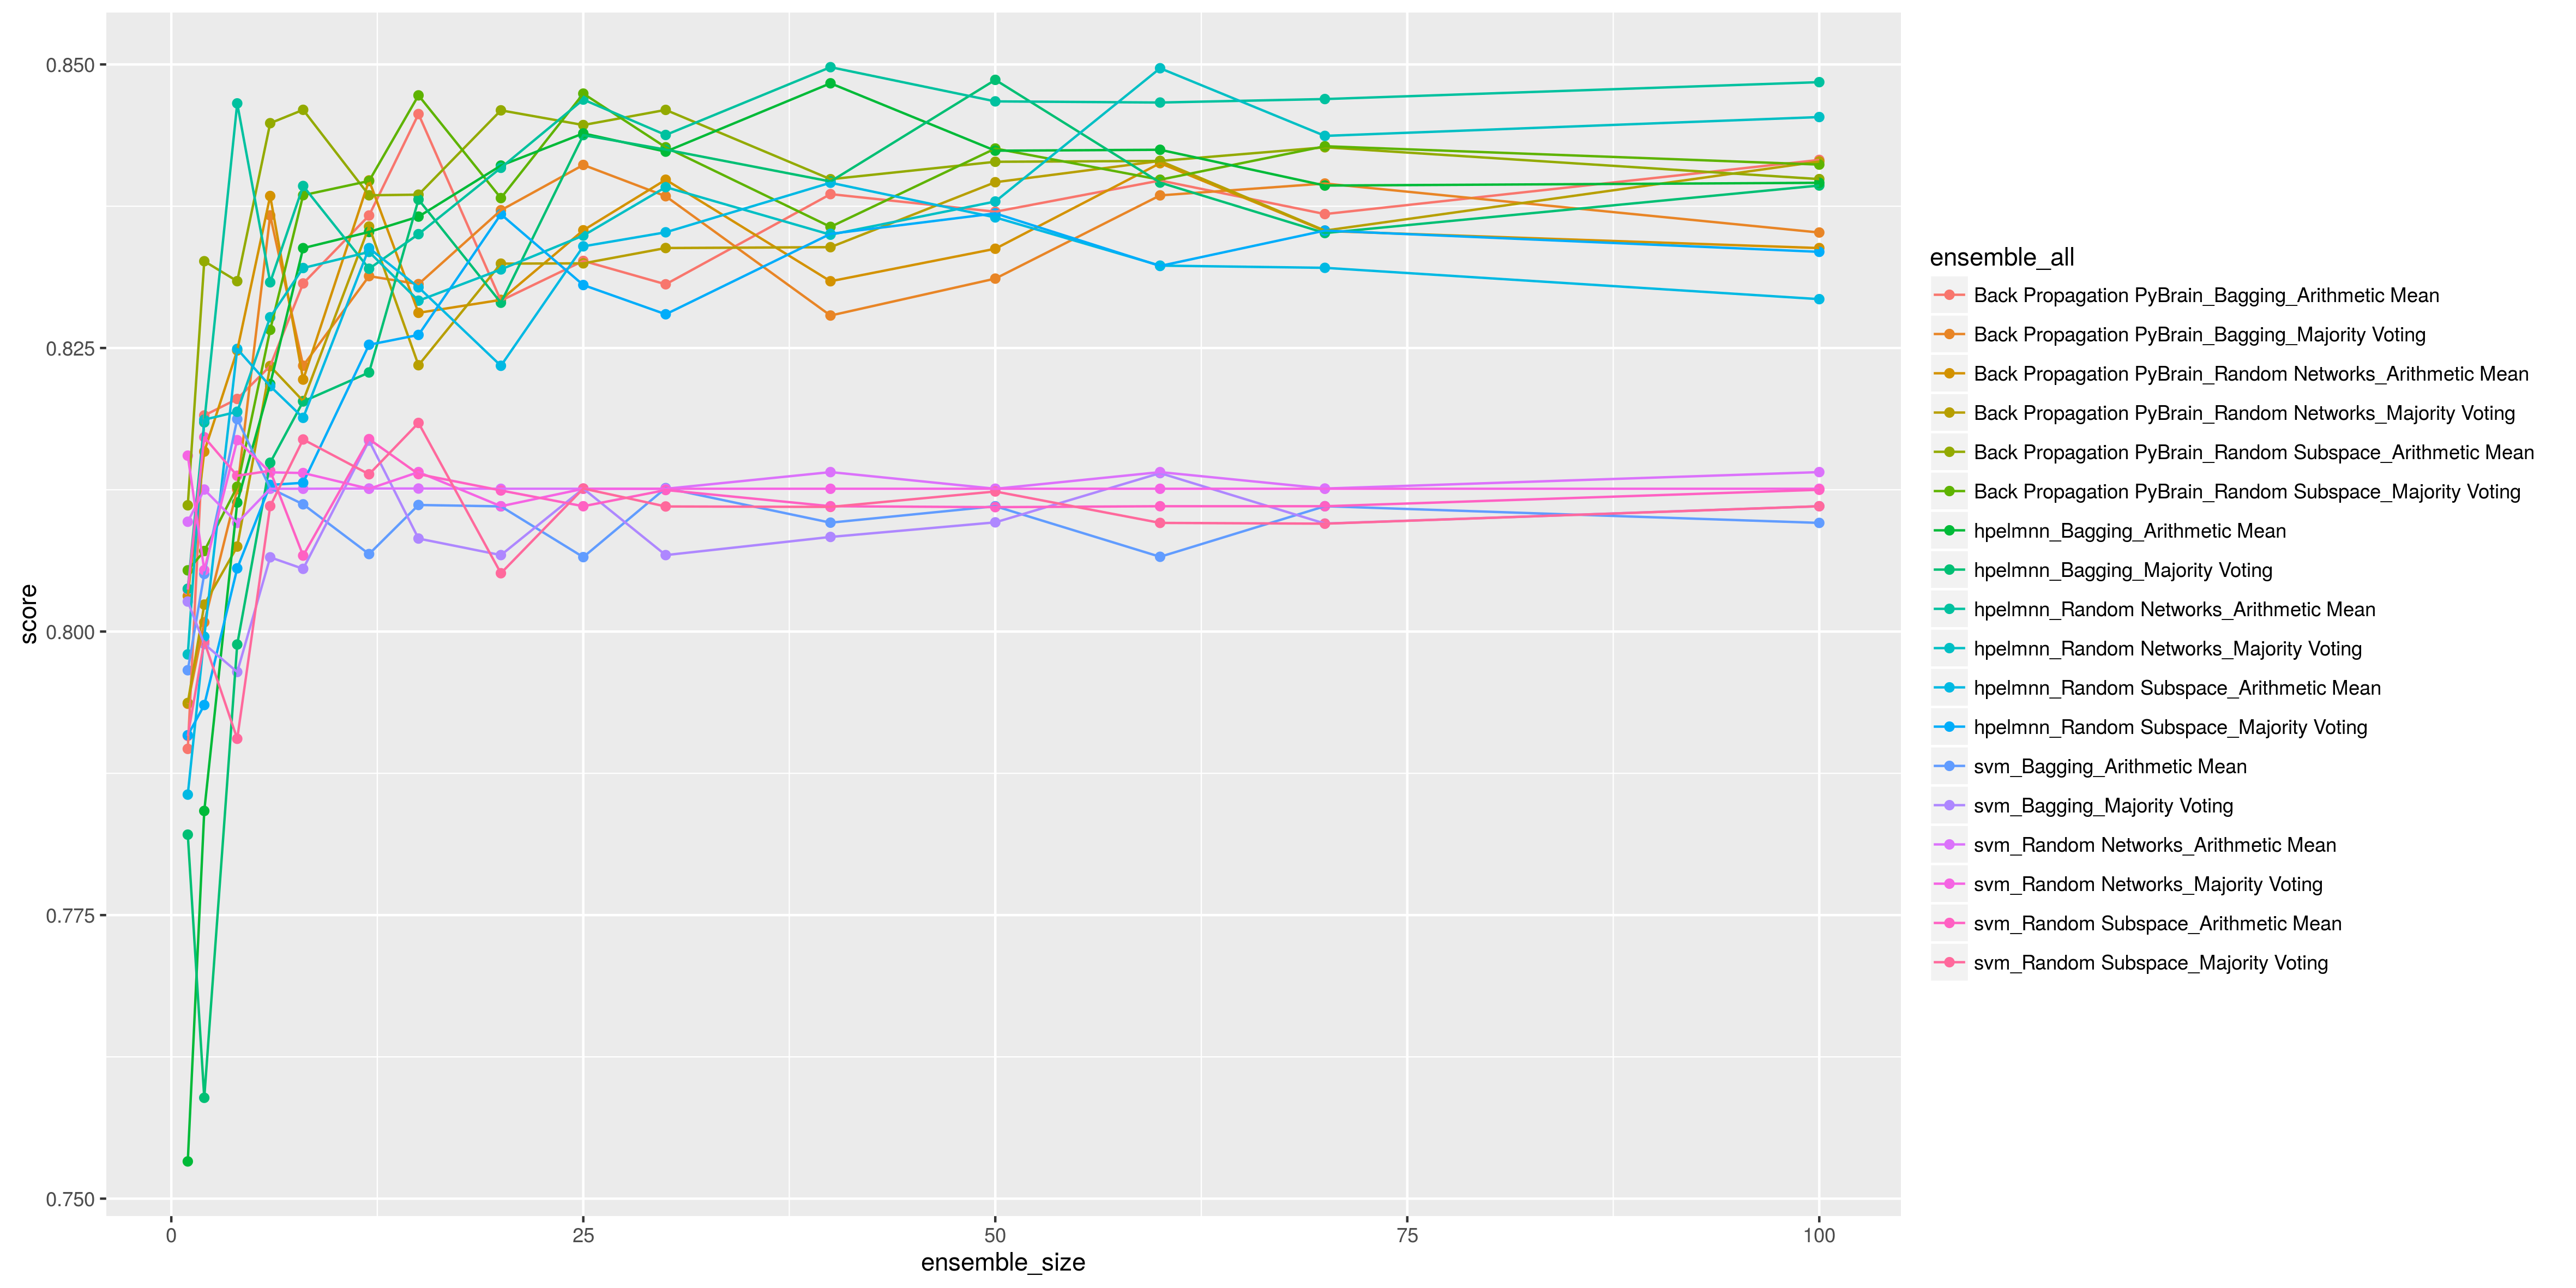
\includegraphics[width=1.0\textwidth]{type3_score_size_dataset_urban_land_cover}\centering\caption{urban\_land\_cover}\end{figure}
\begin{figure}[H]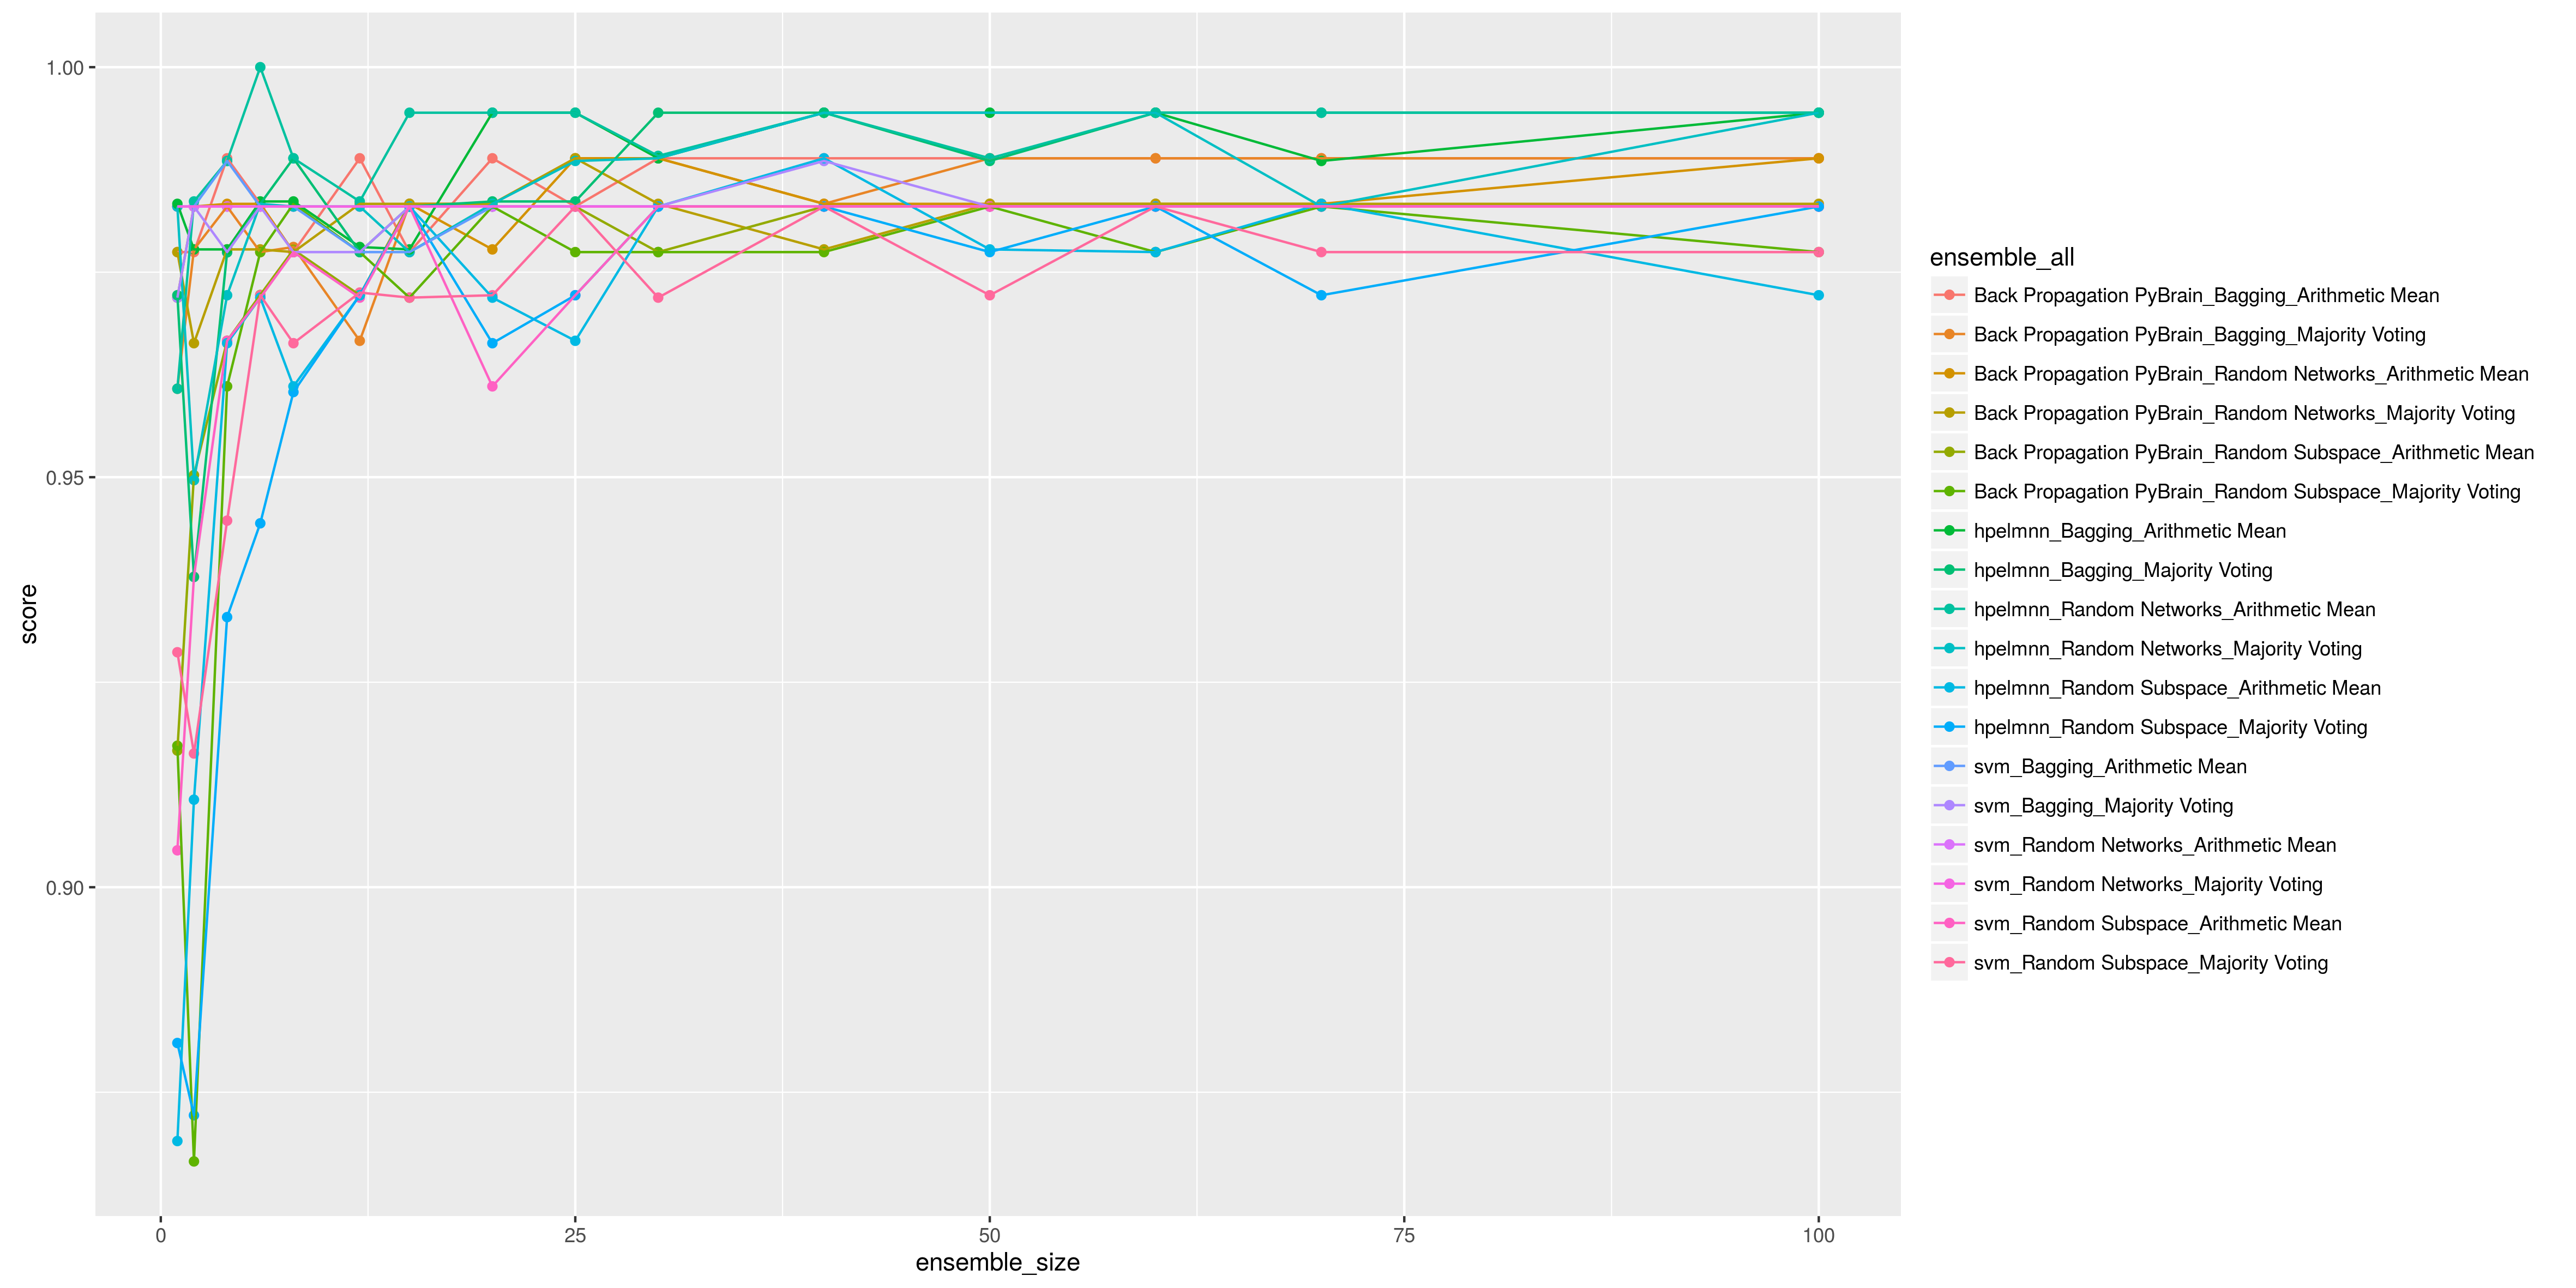
\includegraphics[width=1.0\textwidth]{type3_score_size_dataset_wine}\centering\caption{wine}\end{figure}
\begin{figure}[H]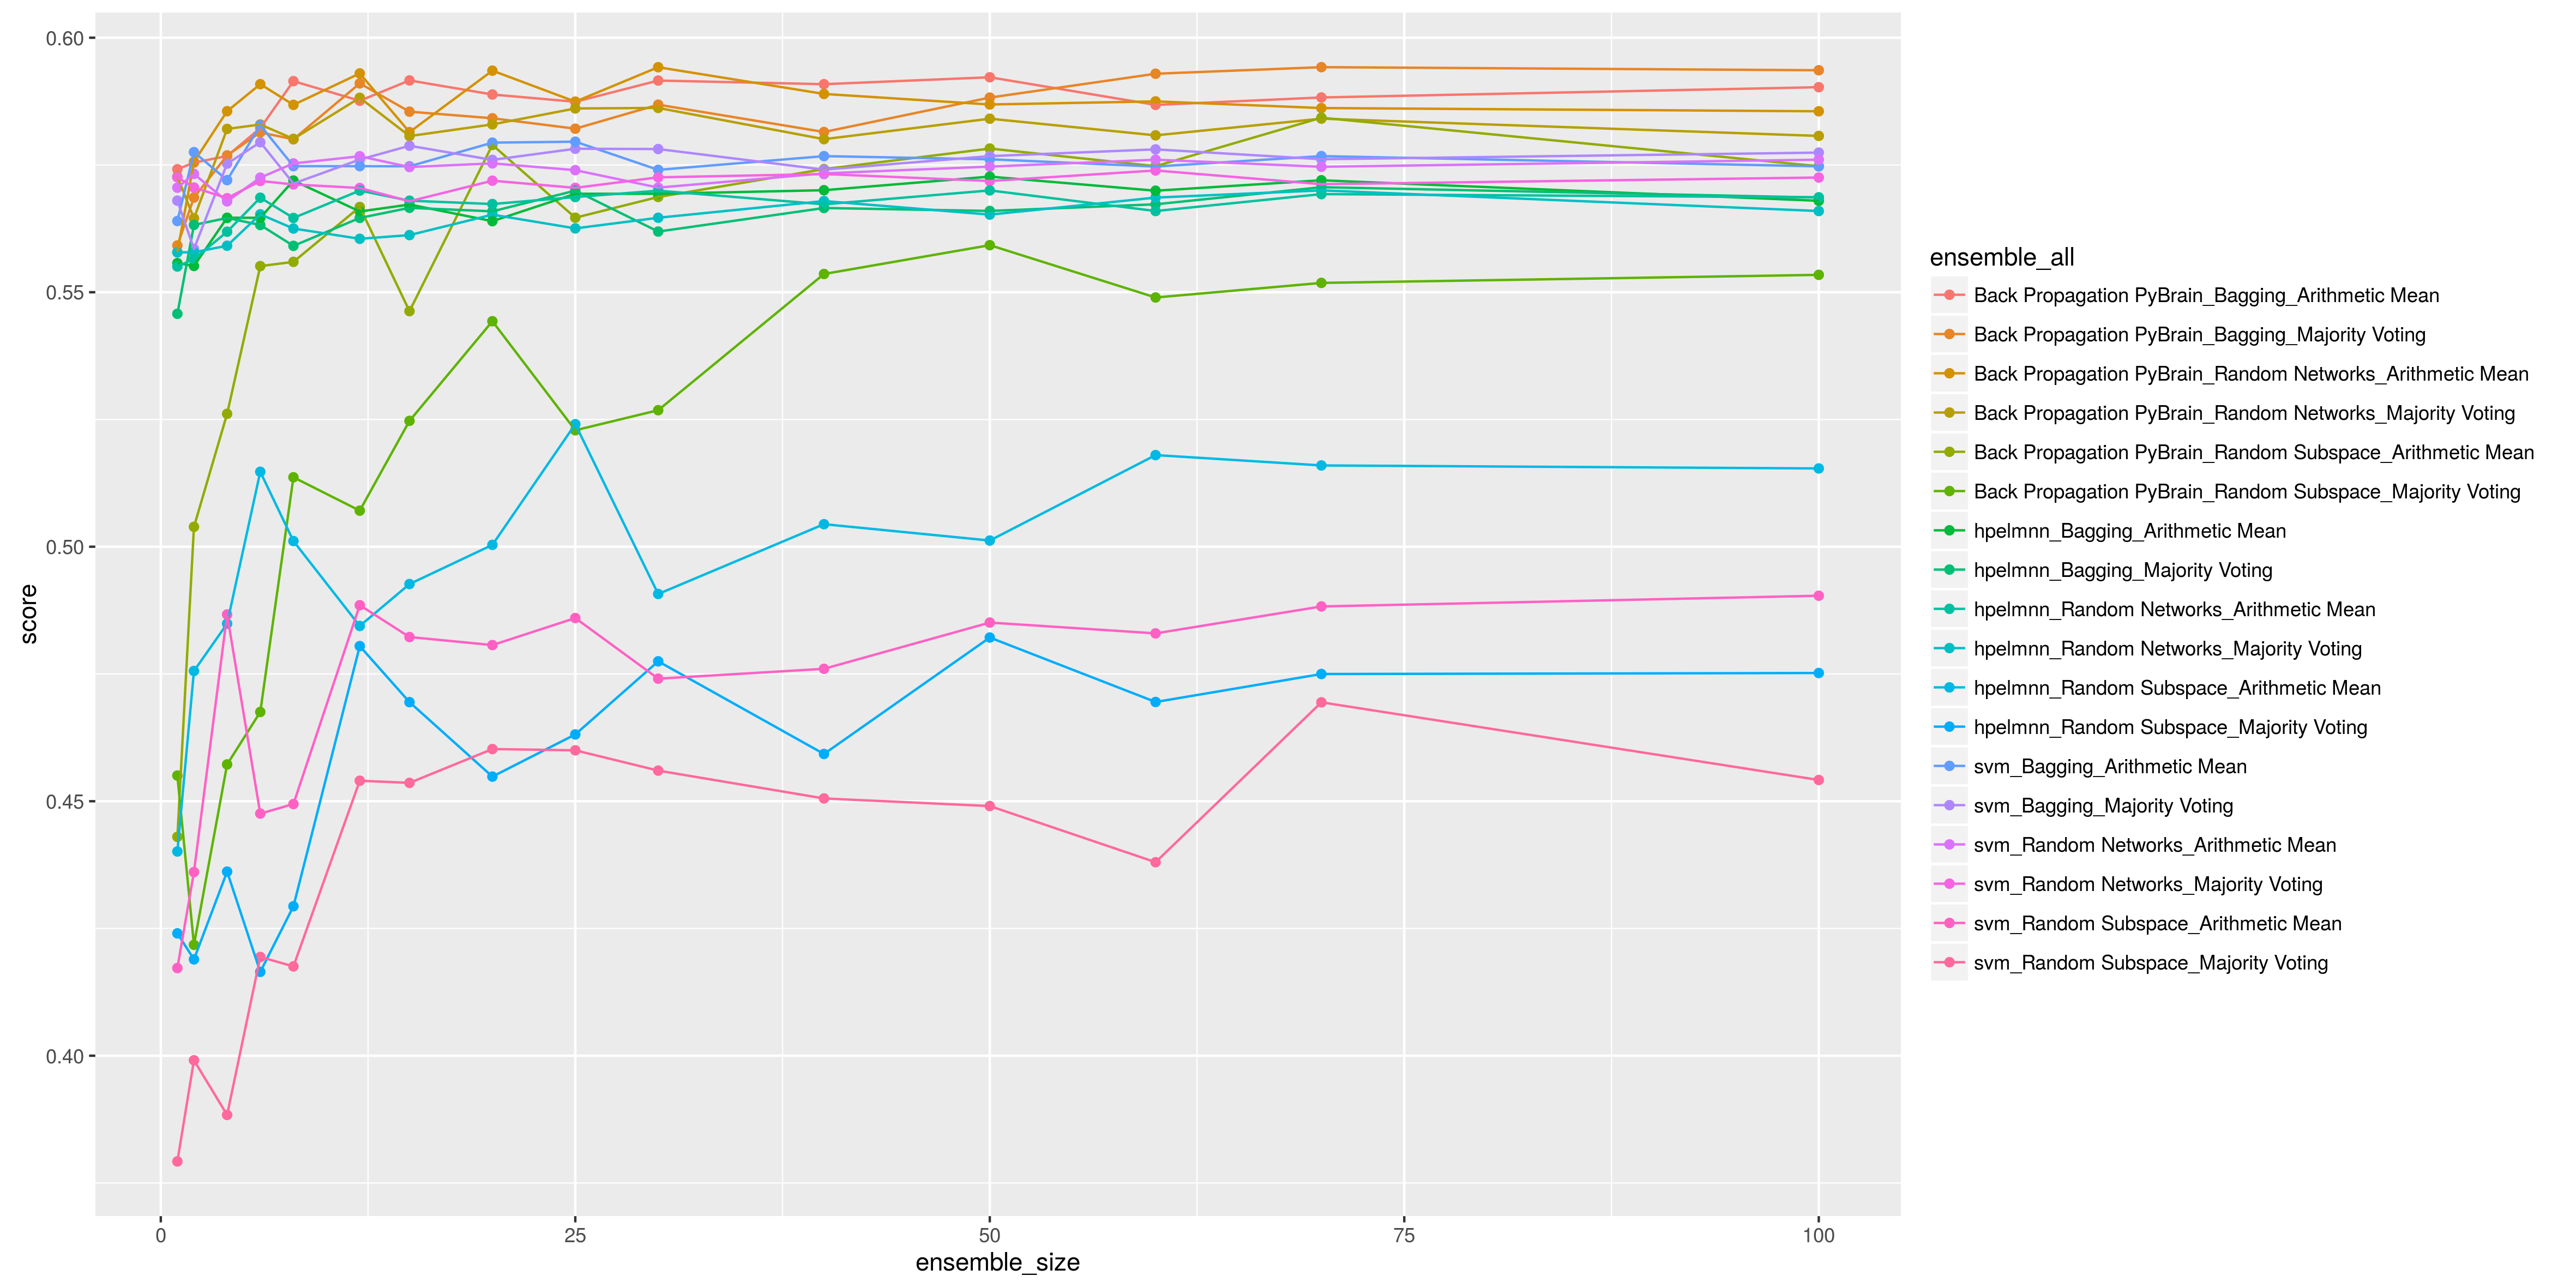
\includegraphics[width=1.0\textwidth]{type3_score_size_dataset_yeast}\centering\caption{yeast}\end{figure}

\begin{figure}[H]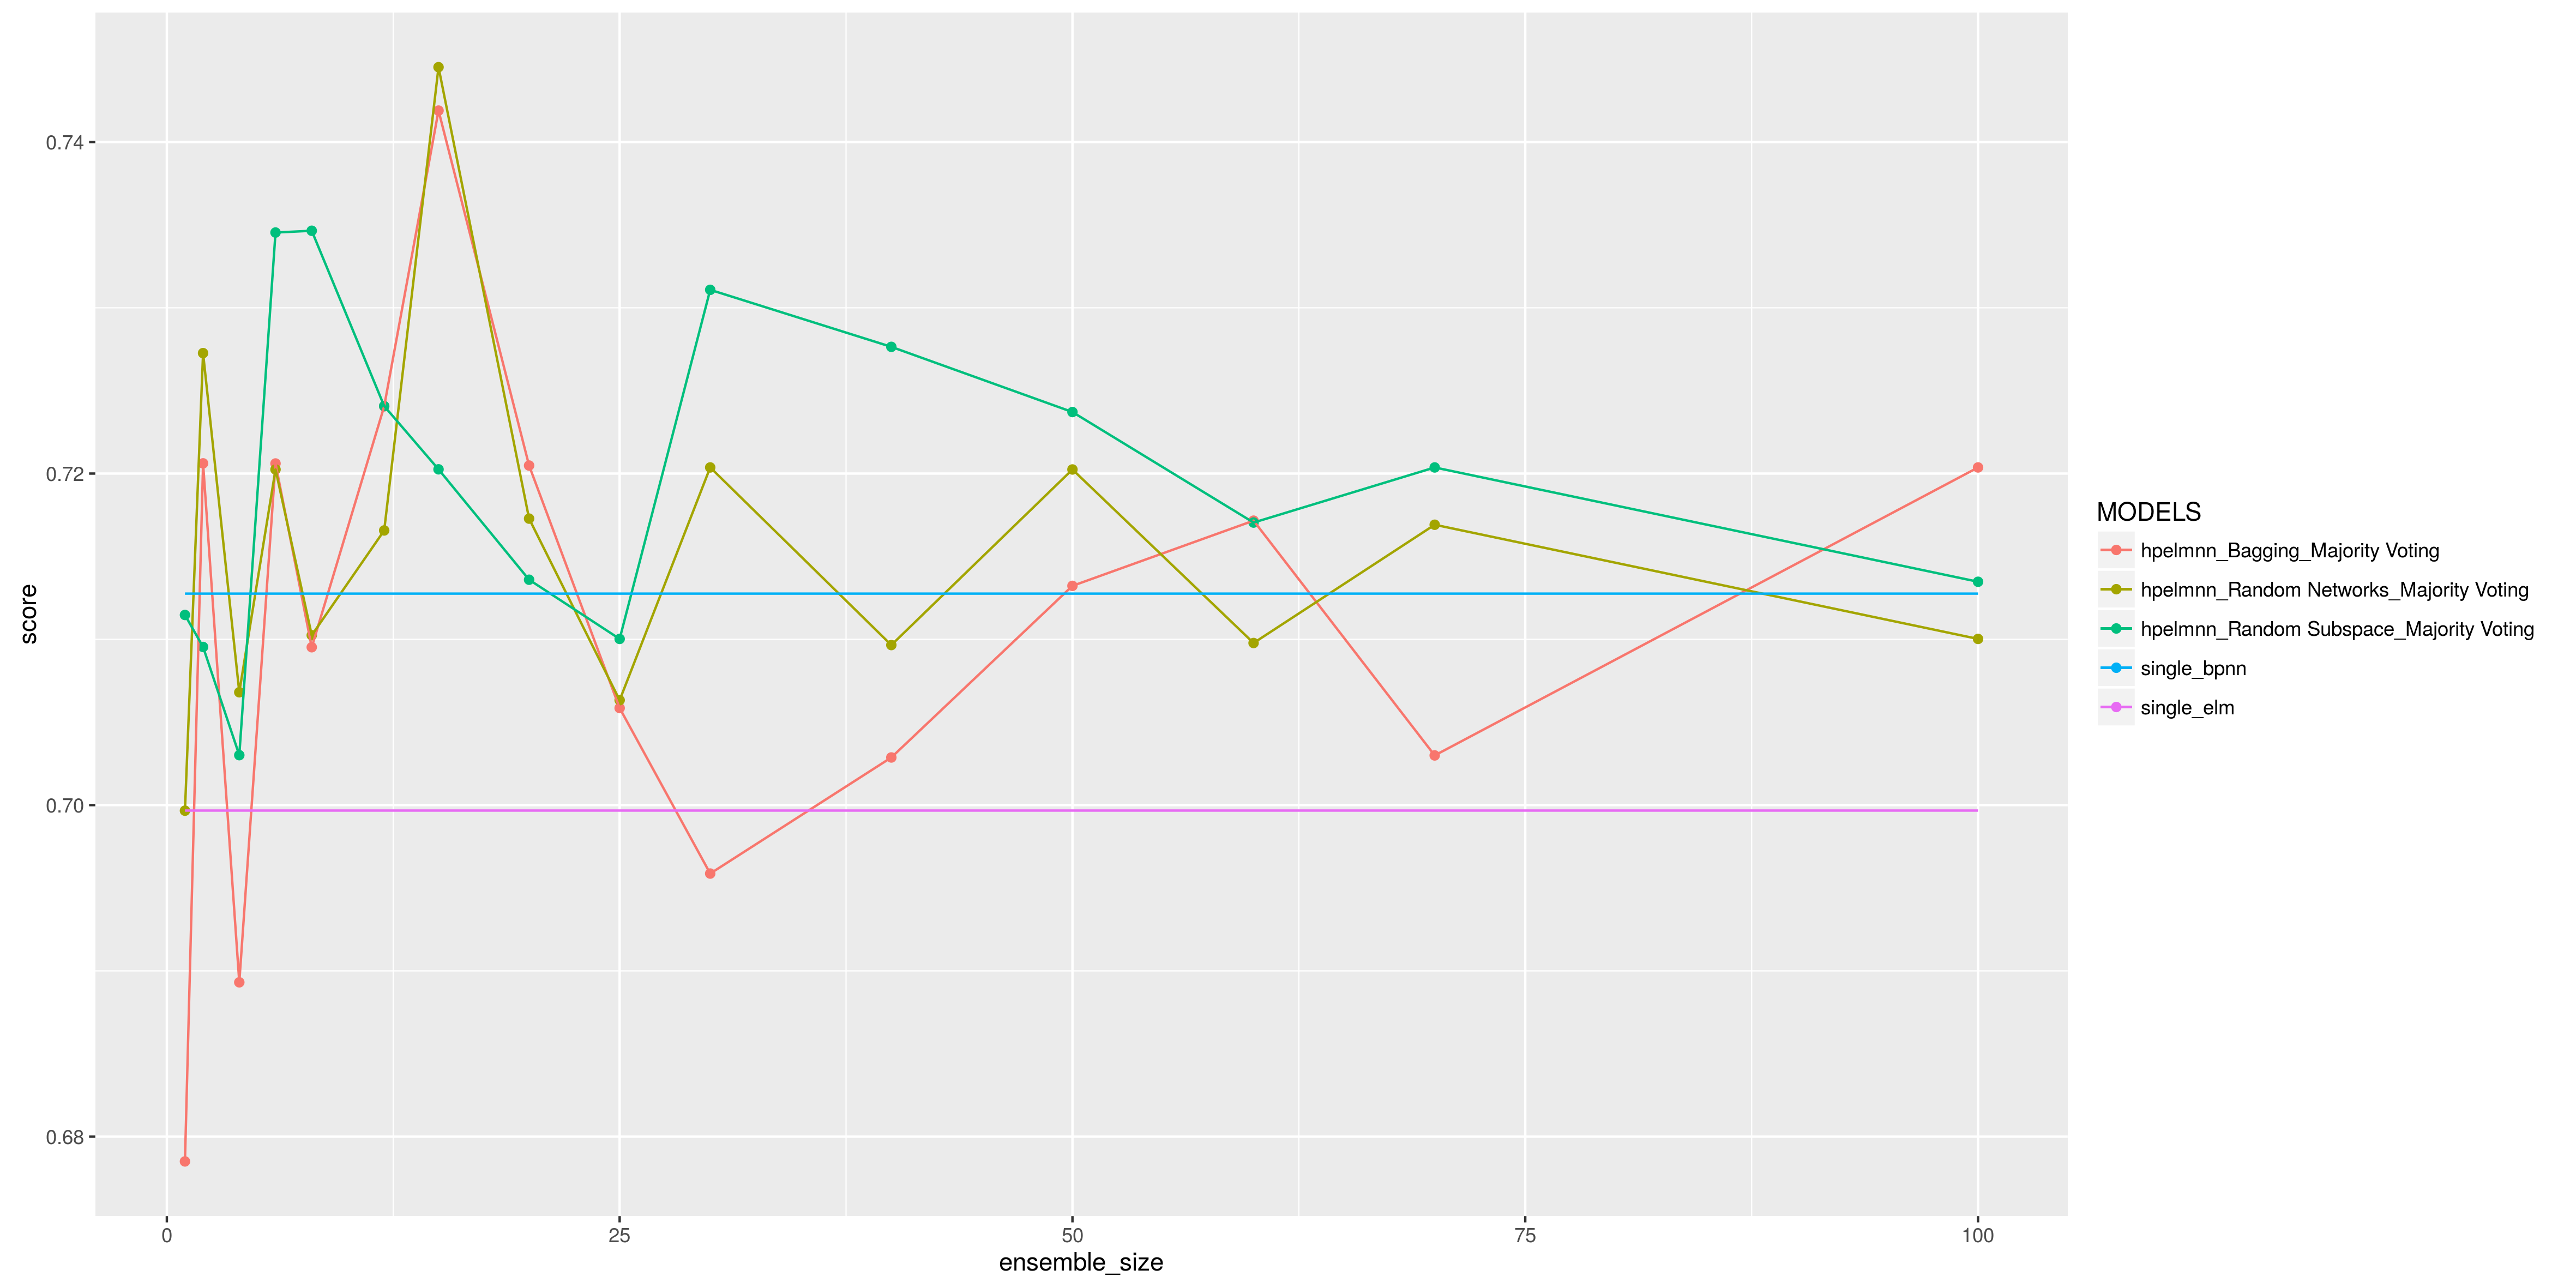
\includegraphics[width=1.0\textwidth]{type4_primary_task_dataset_breast_cancer}\centering\caption{breast\_cancer}\end{figure}
\begin{figure}[H]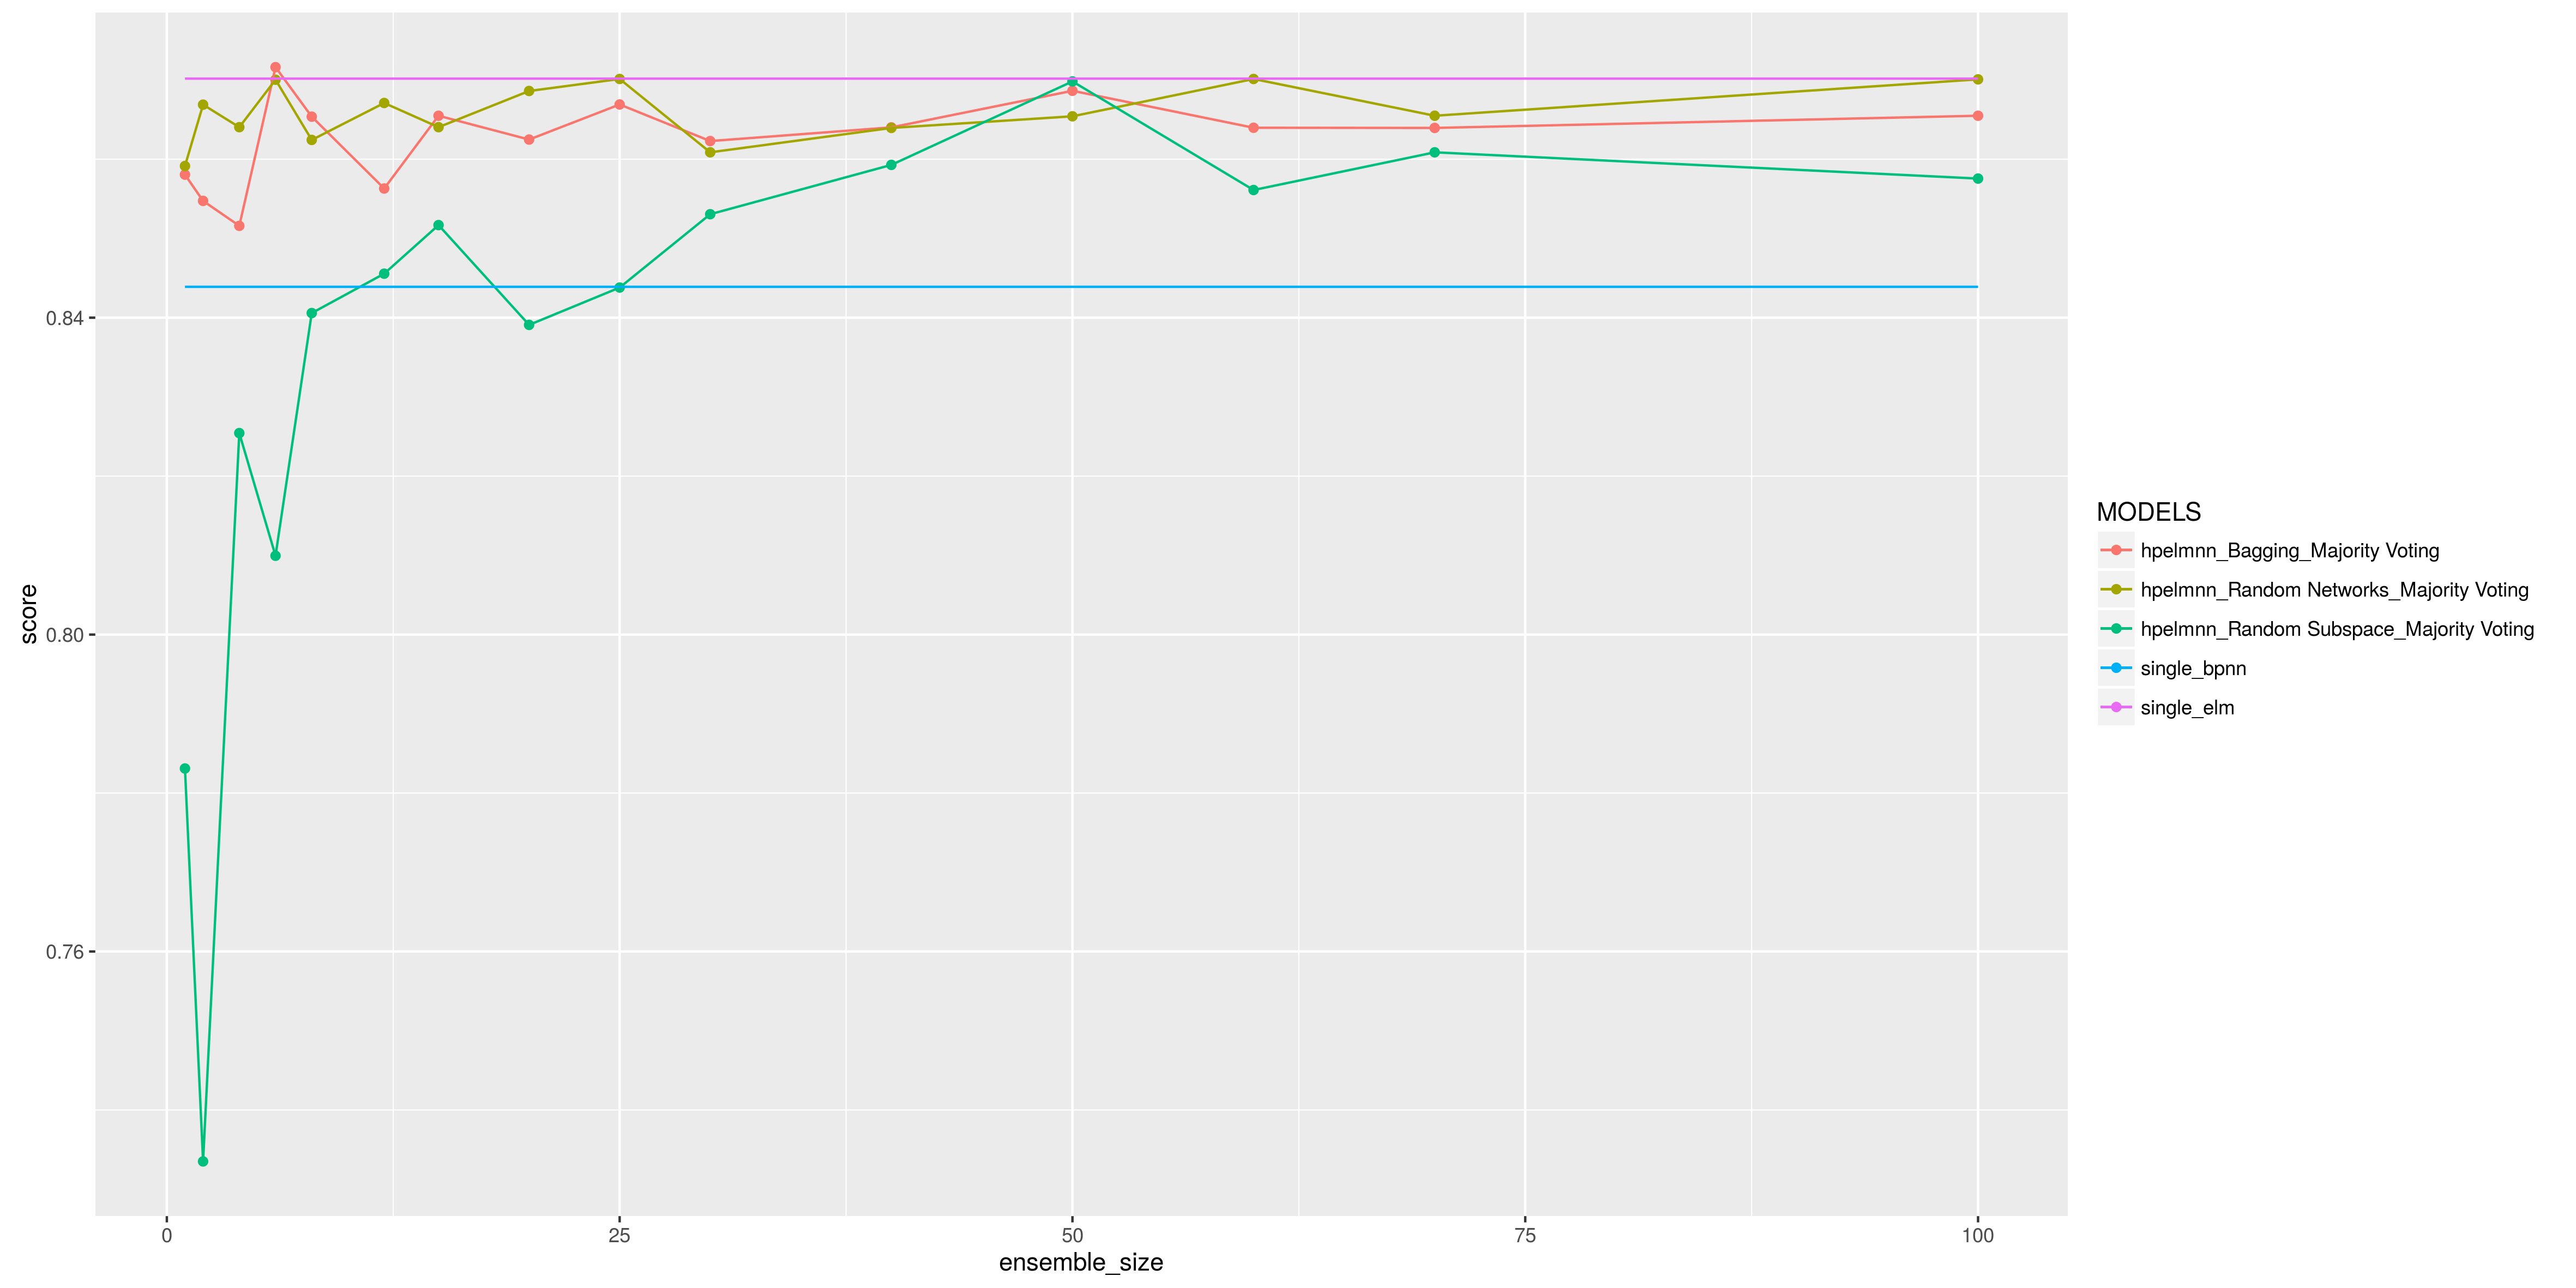
\includegraphics[width=1.0\textwidth]{type4_primary_task_dataset_crx}\centering\caption{crx}\end{figure}
\begin{figure}[H]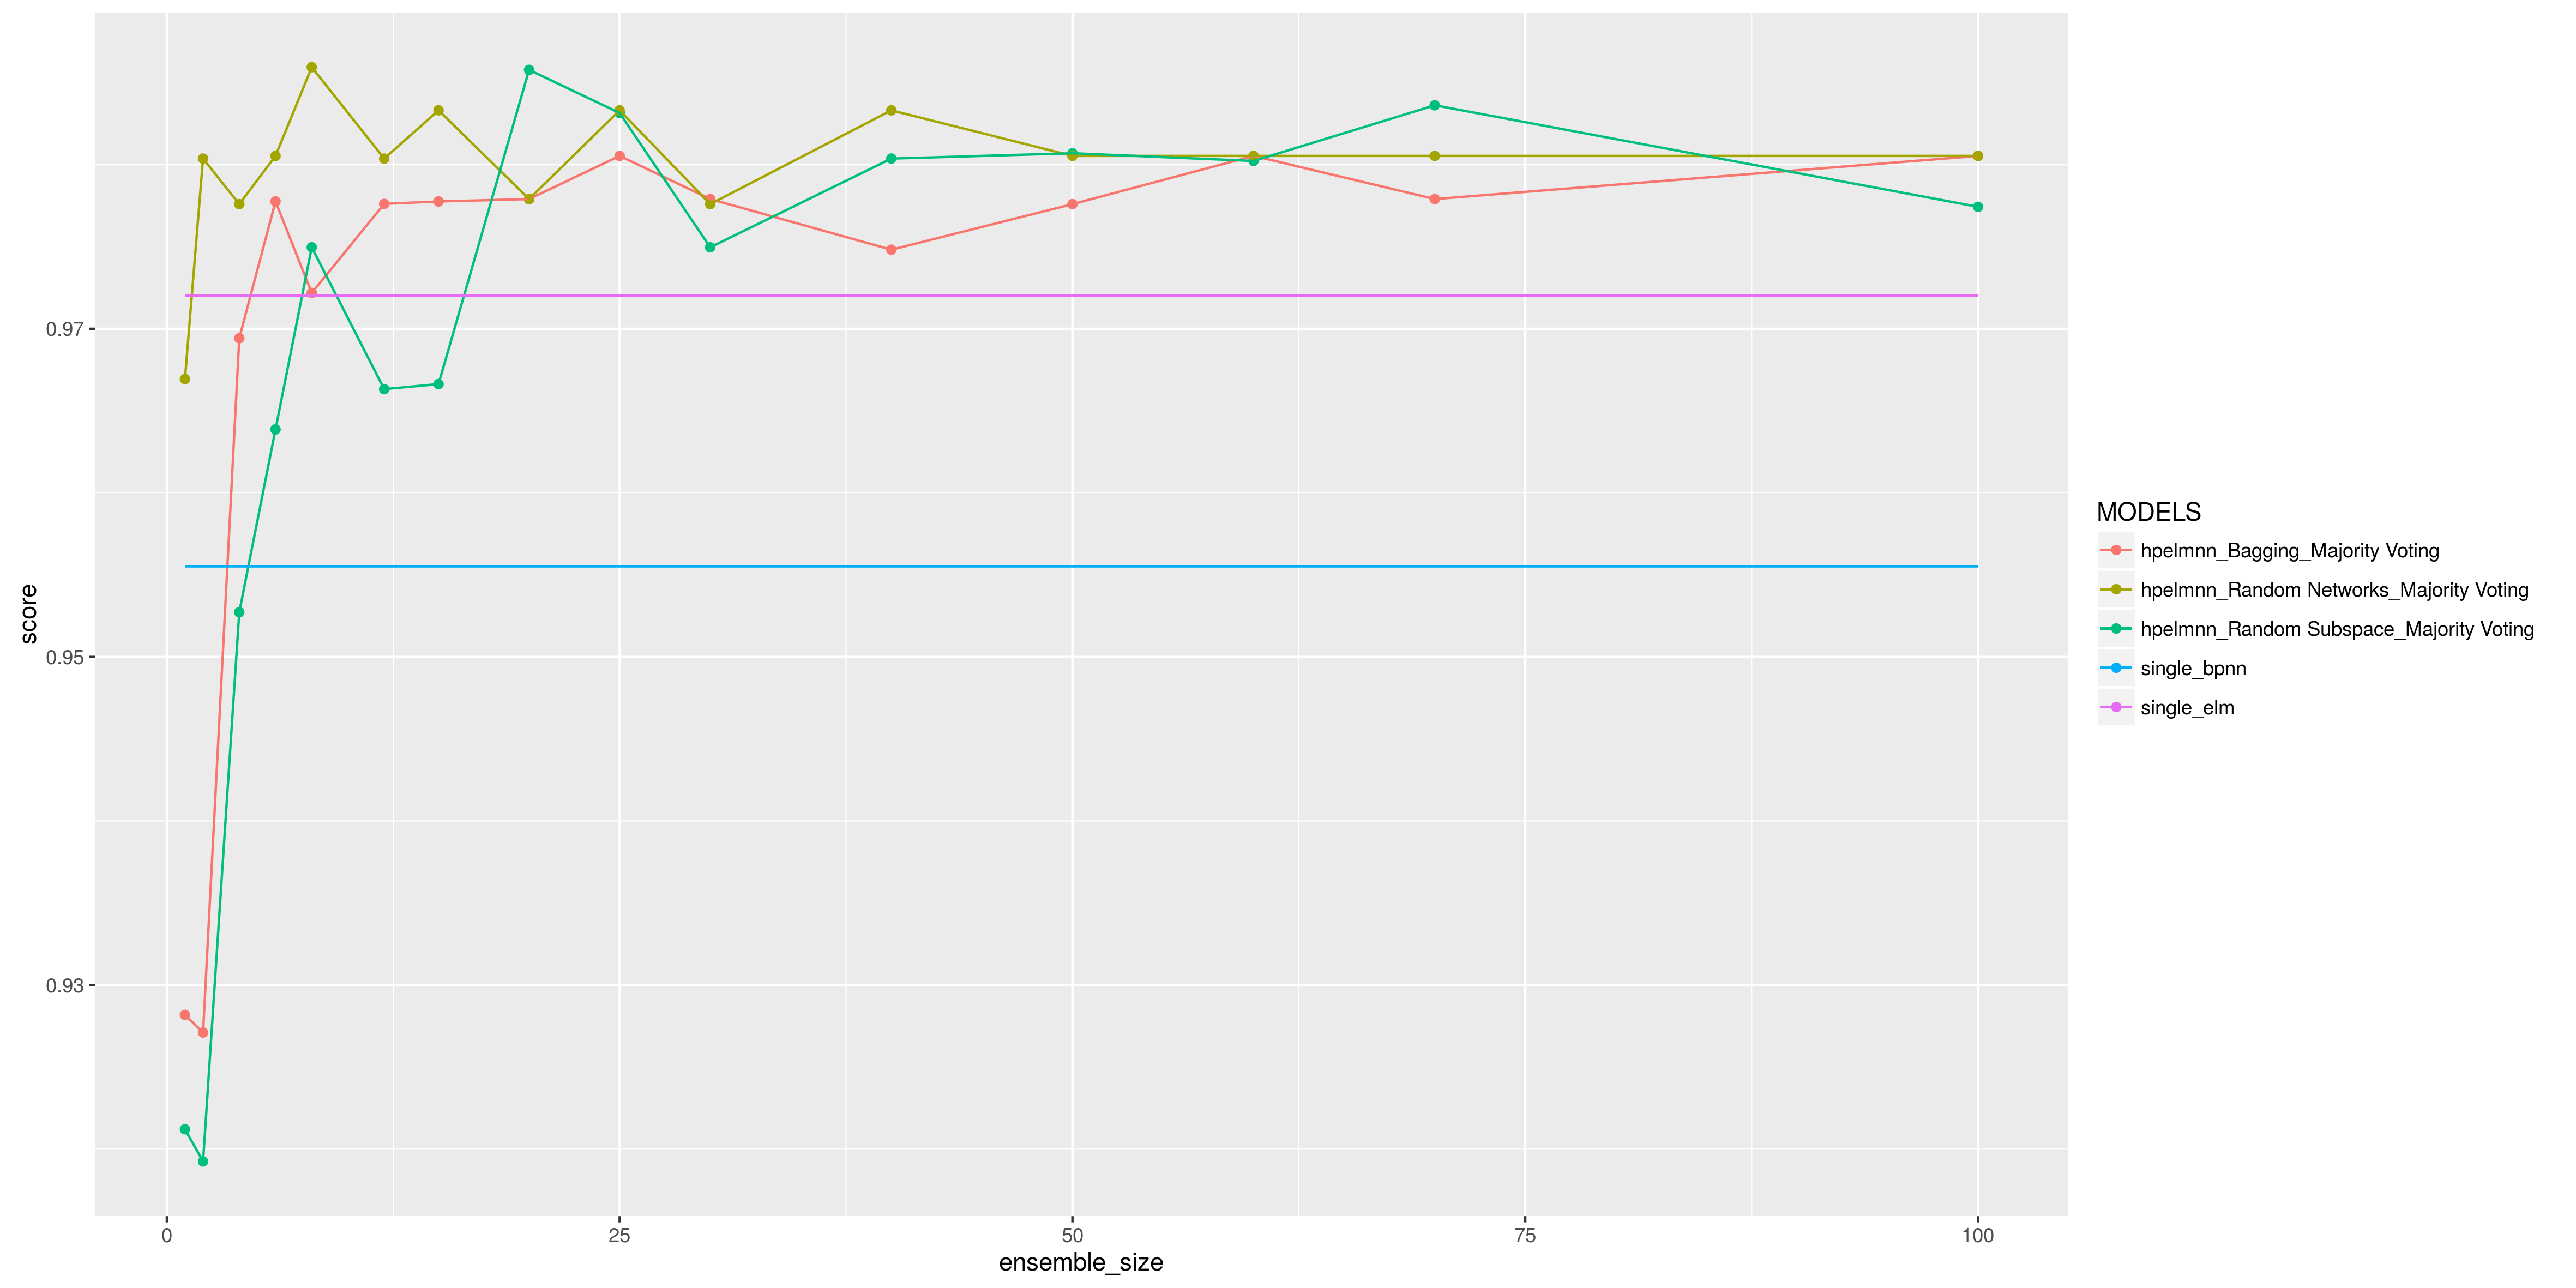
\includegraphics[width=1.0\textwidth]{type4_primary_task_dataset_dermatology}\centering\caption{dermatology}\end{figure}
\begin{figure}[H]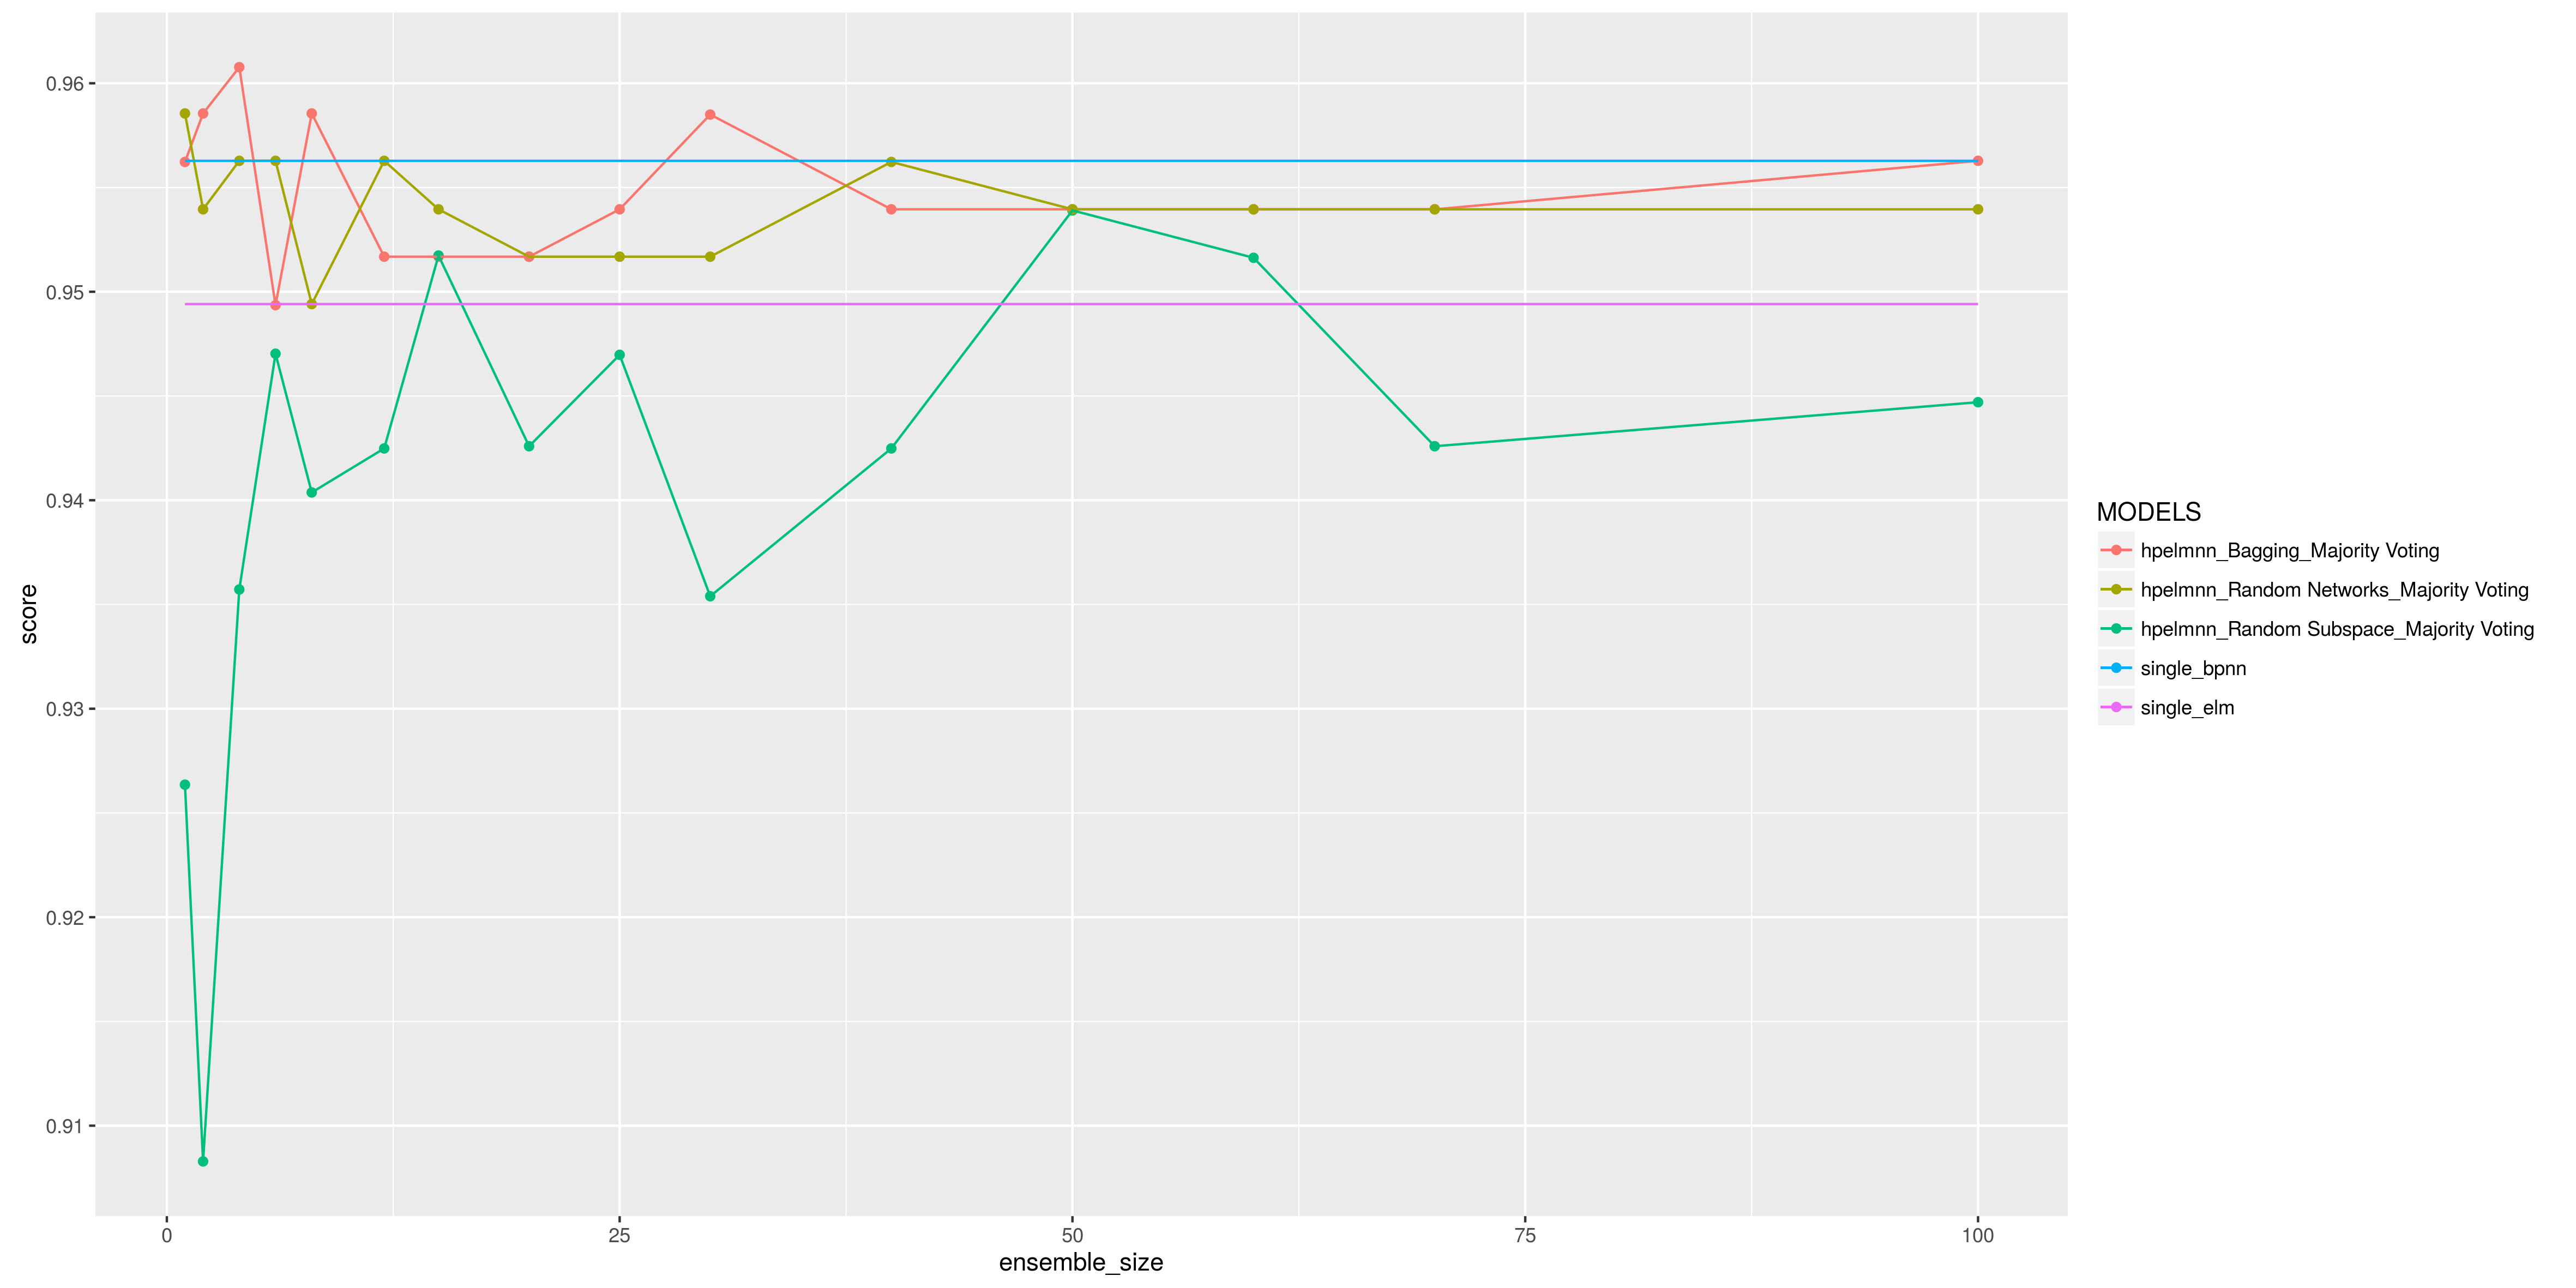
\includegraphics[width=1.0\textwidth]{type4_primary_task_dataset_house_votes}\centering\caption{house\_votes}\end{figure}
\begin{figure}[H]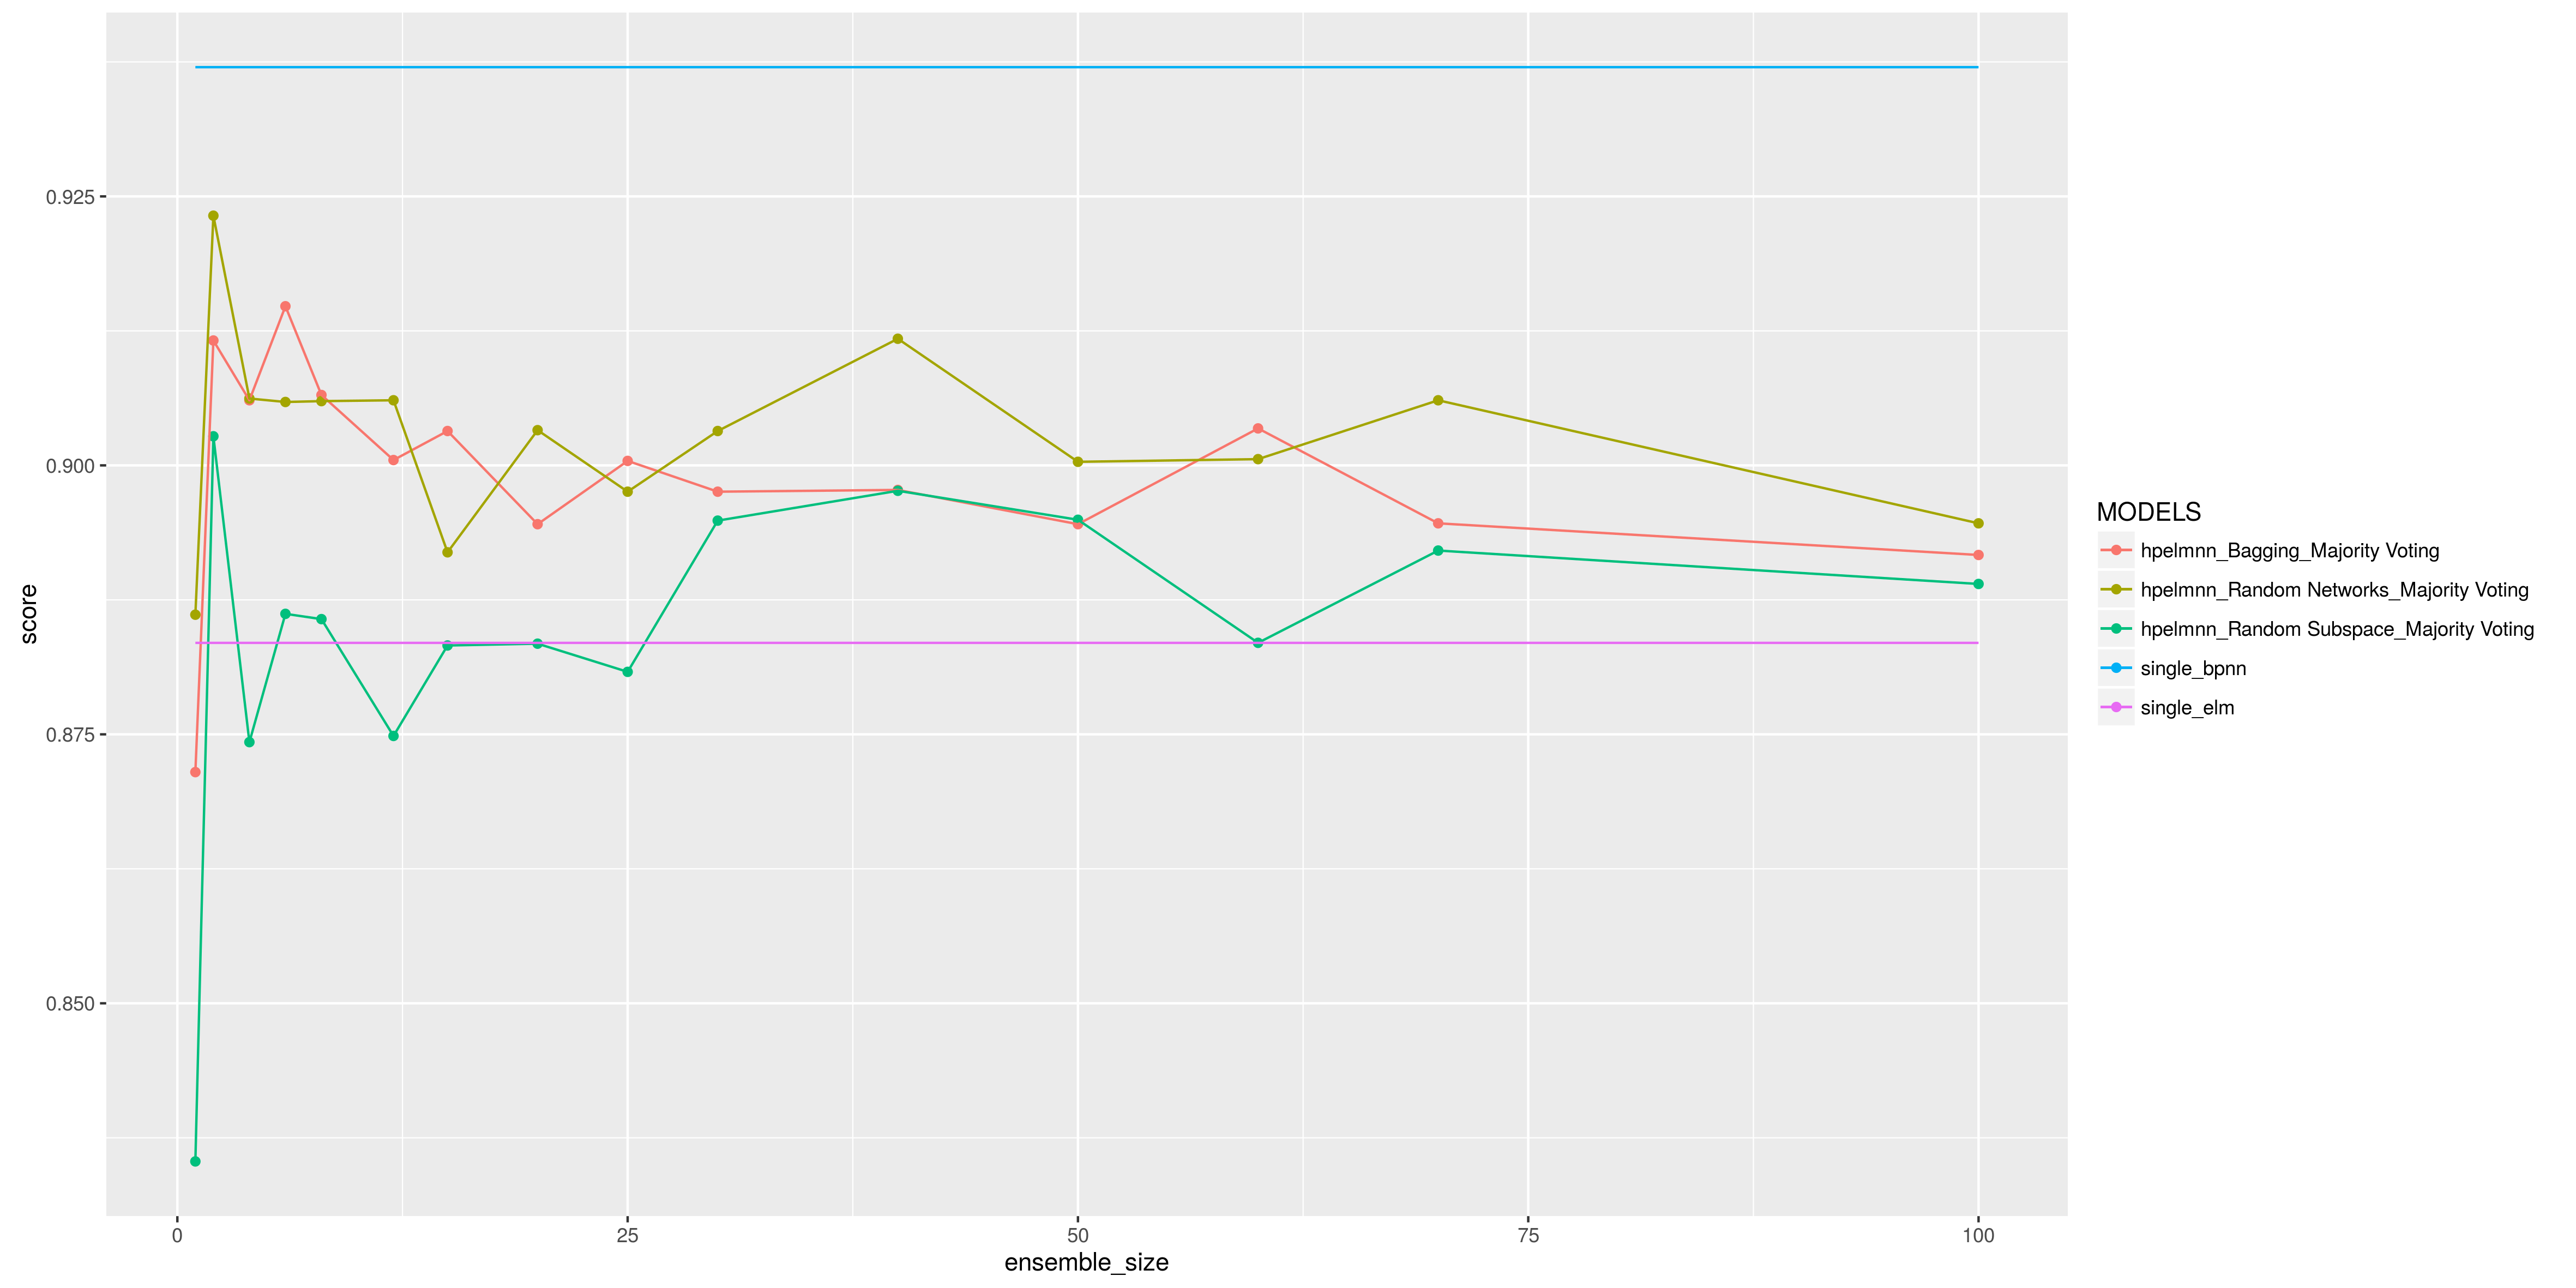
\includegraphics[width=1.0\textwidth]{type4_primary_task_dataset_ionosphere}\centering\caption{ionosphere}\end{figure}
\begin{figure}[H]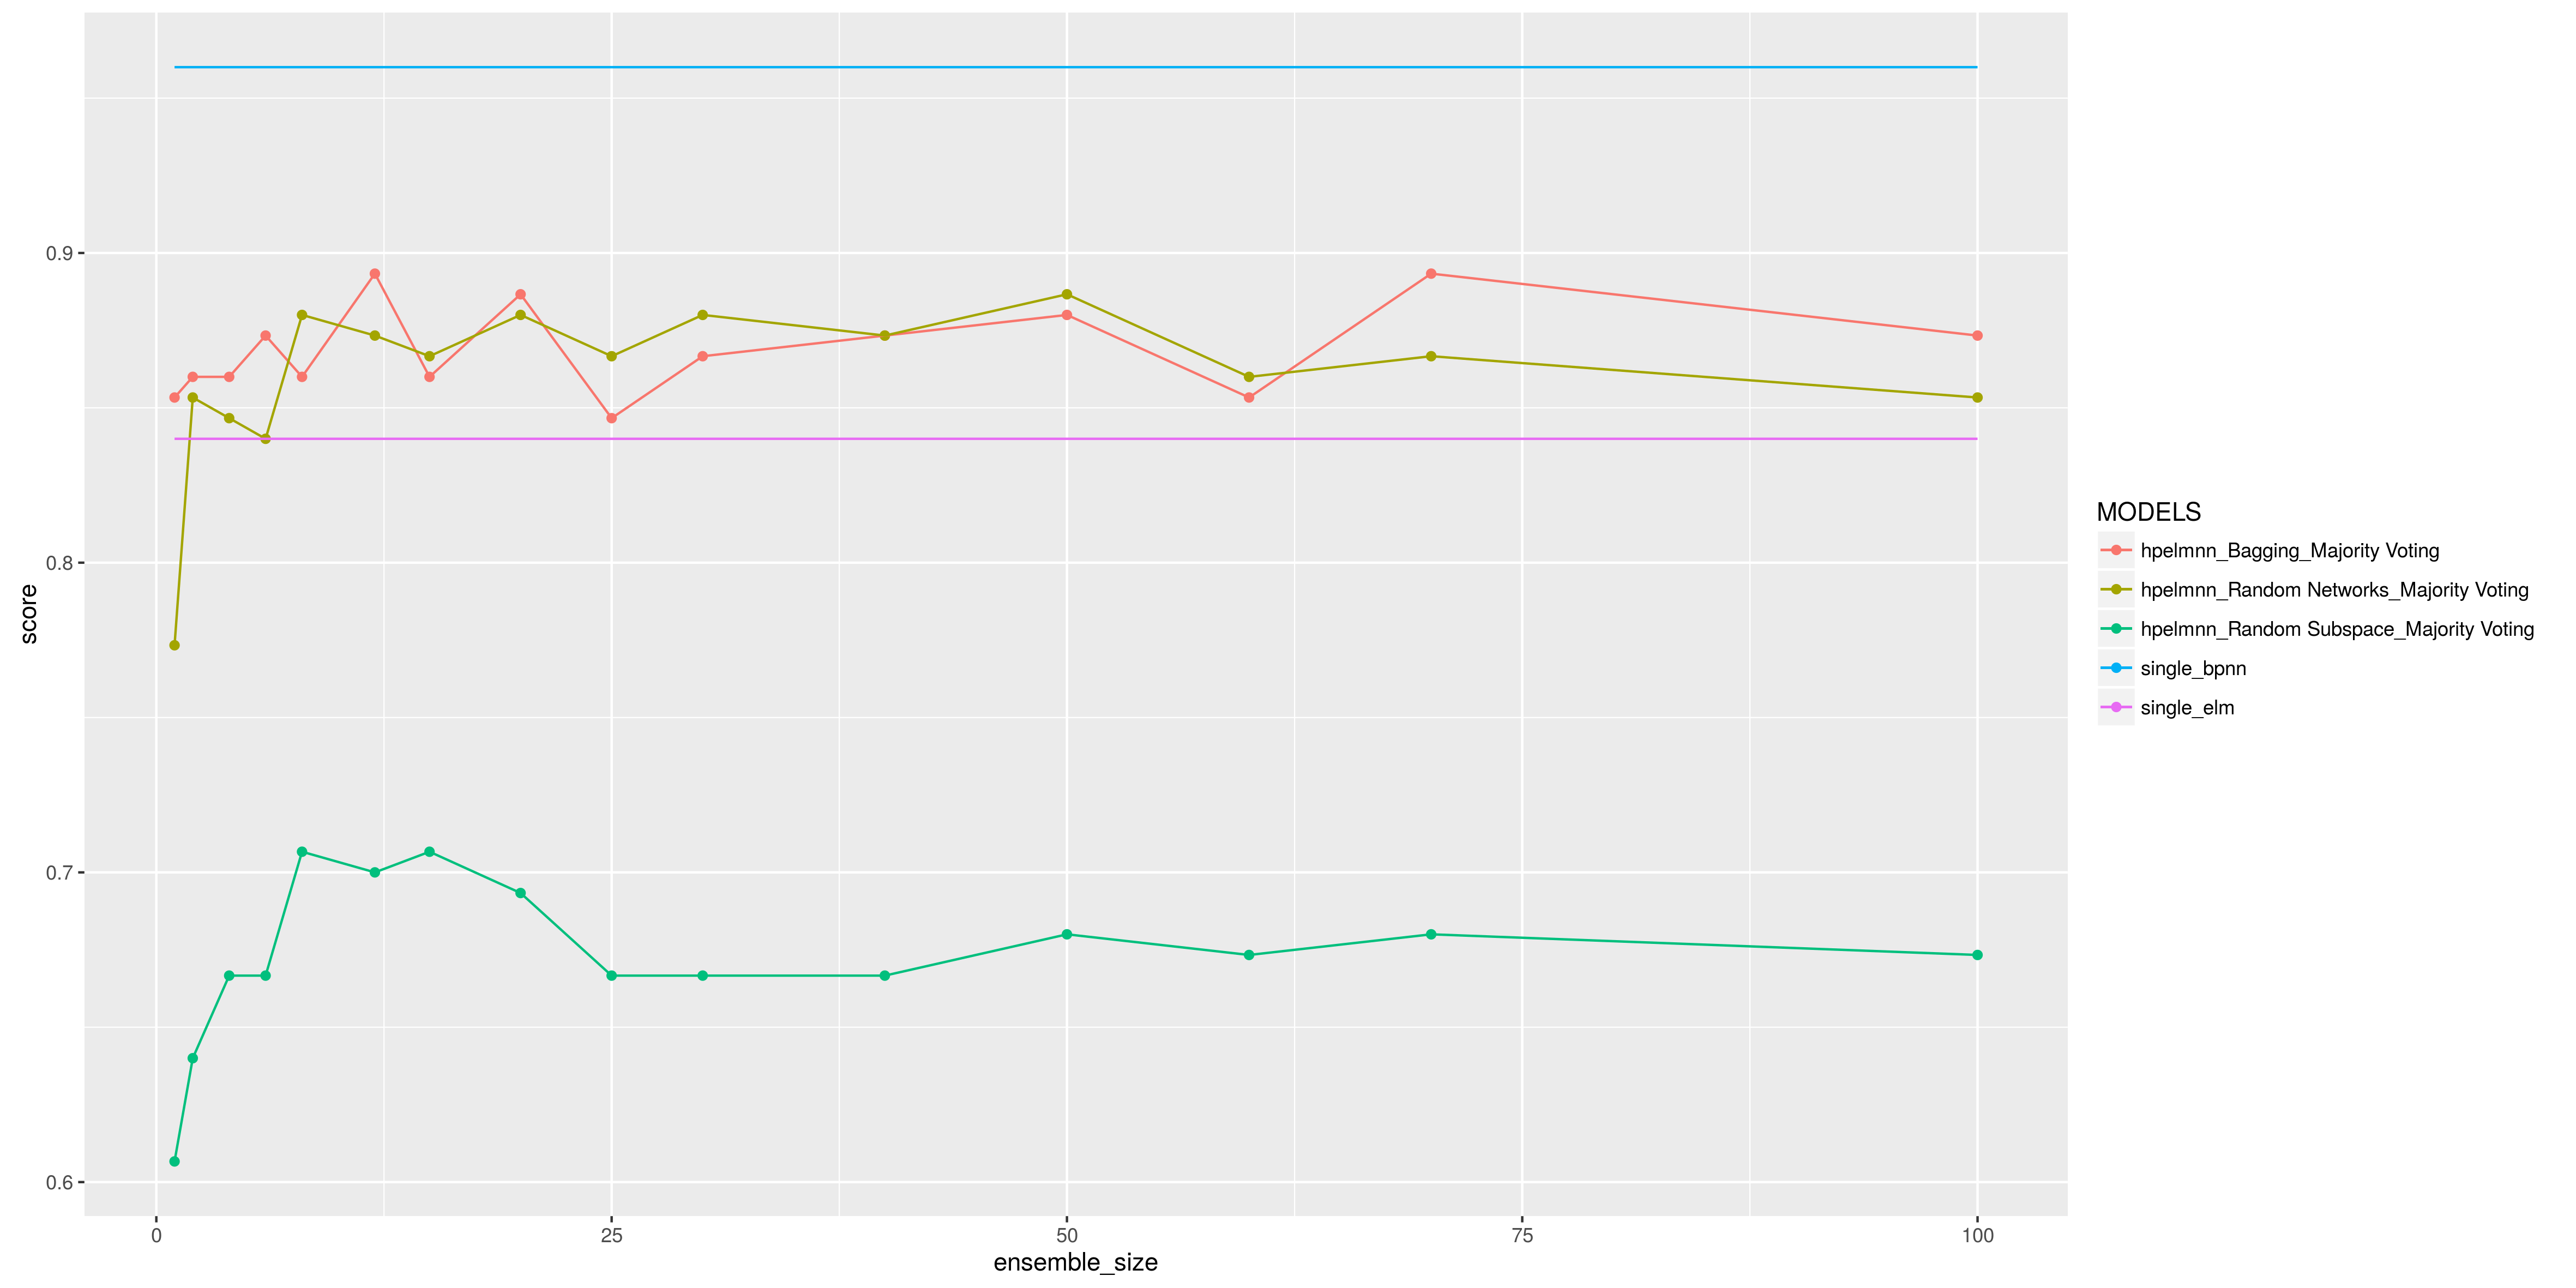
\includegraphics[width=1.0\textwidth]{type4_primary_task_dataset_iris}\centering\caption{iris}\end{figure}
\begin{figure}[H]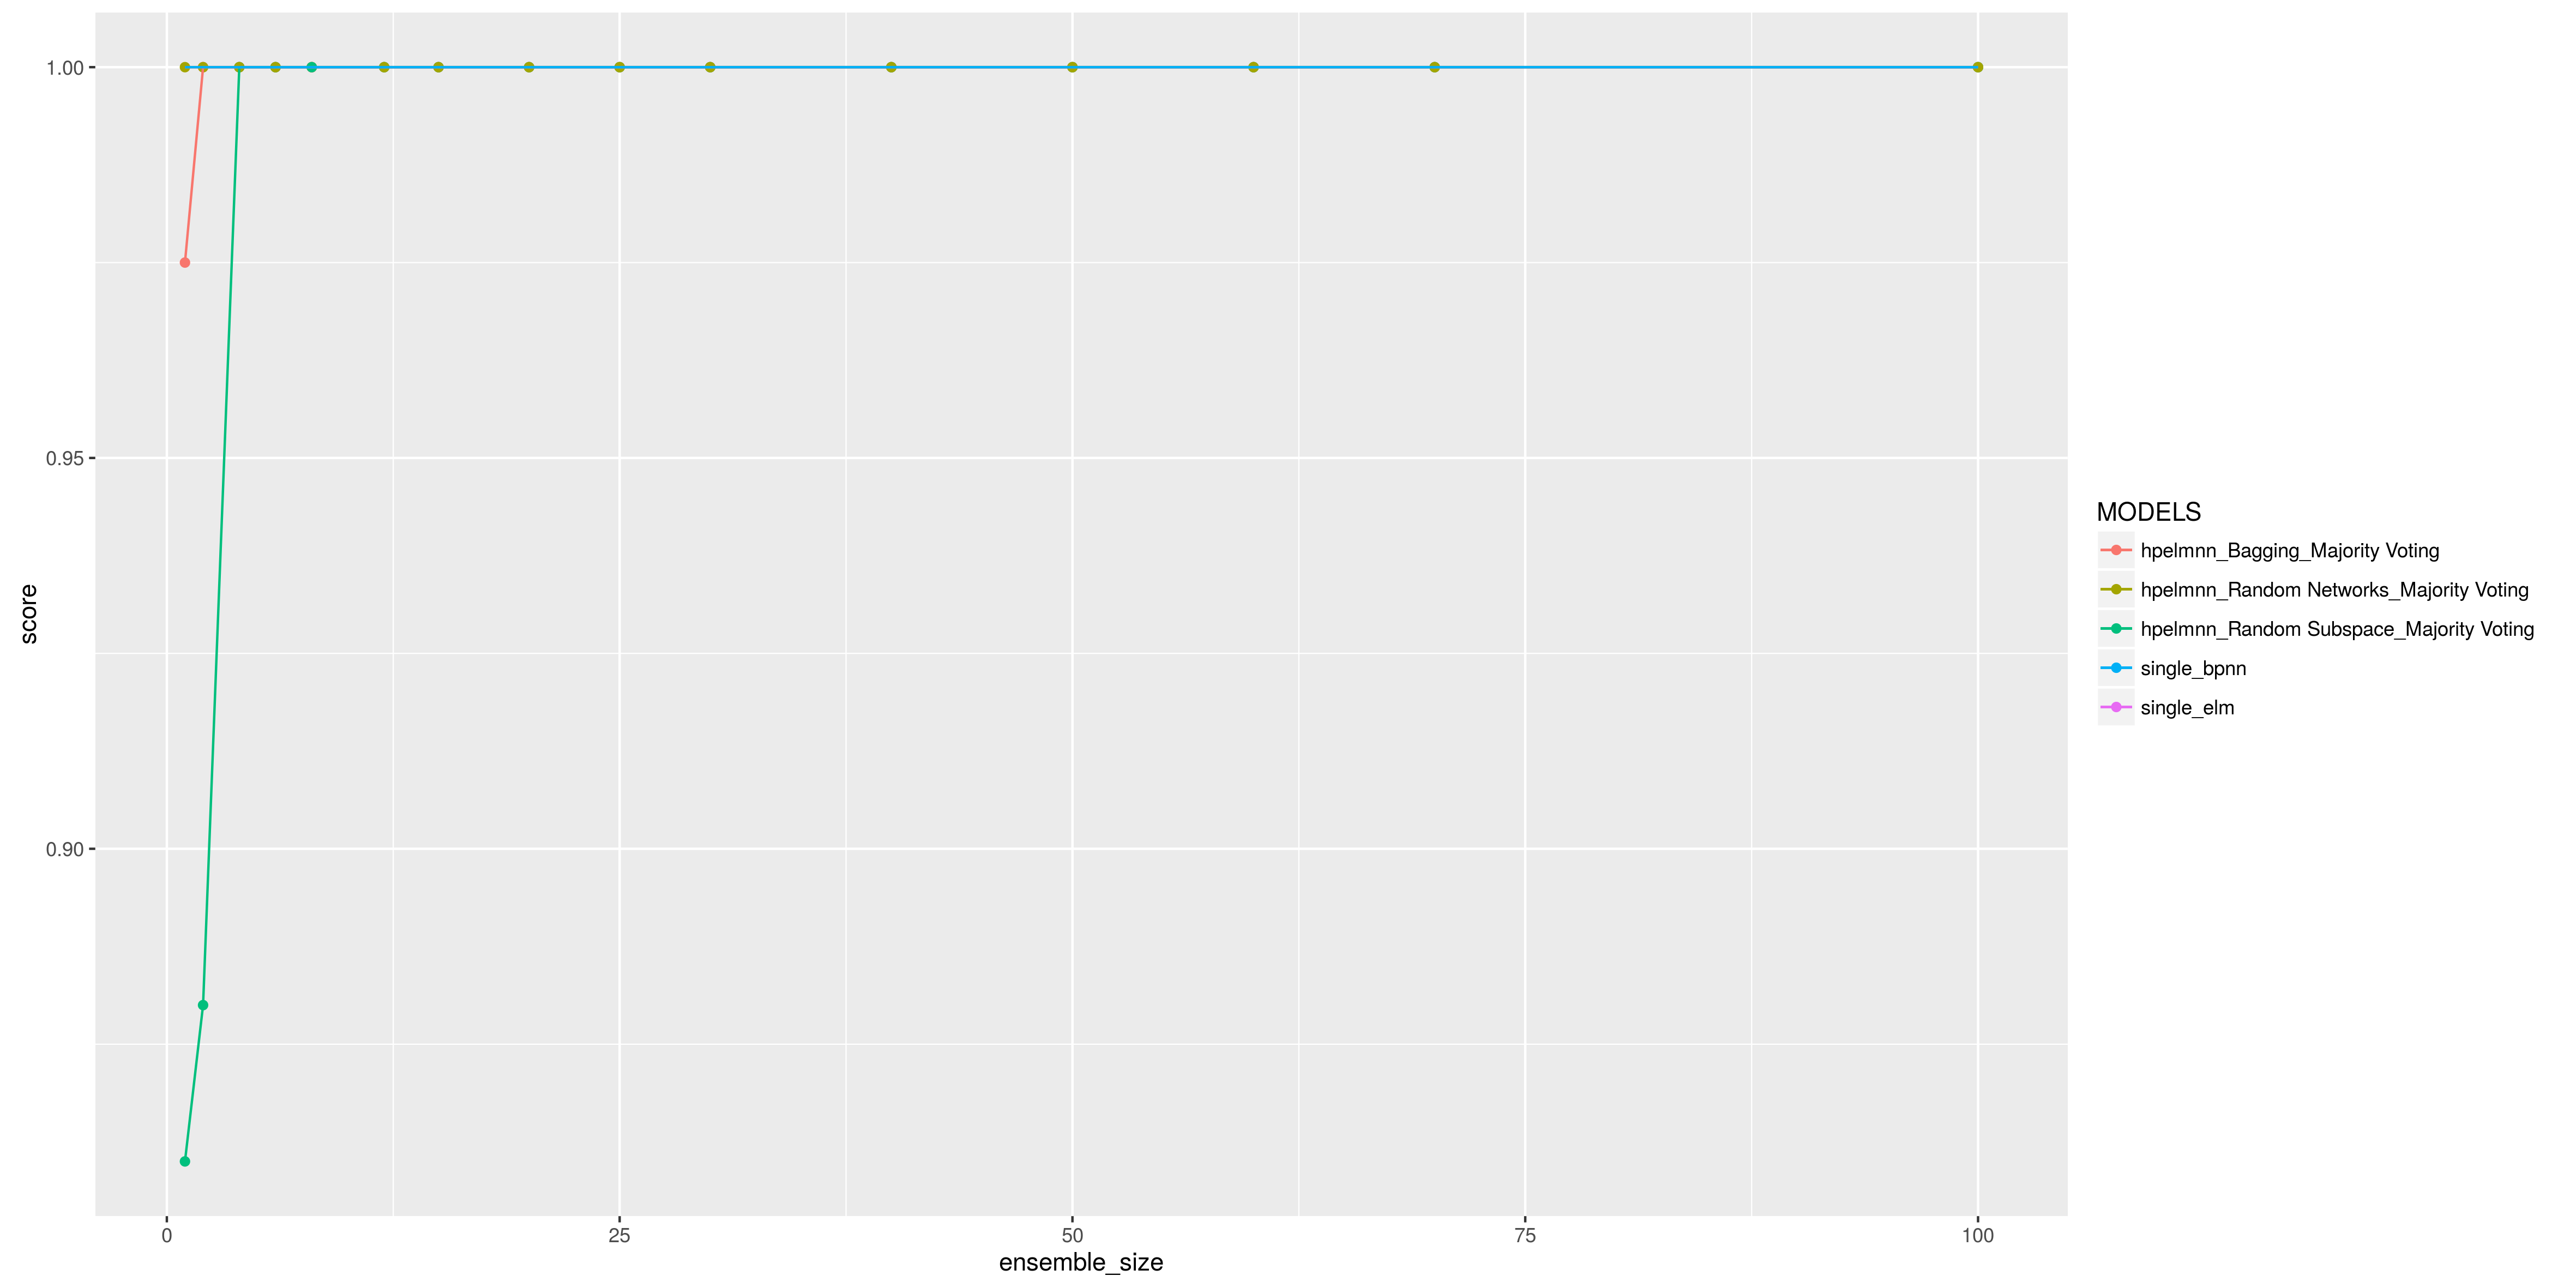
\includegraphics[width=1.0\textwidth]{type4_primary_task_dataset_soybean_small}\centering\caption{soybean\_small}\end{figure}
\begin{figure}[H]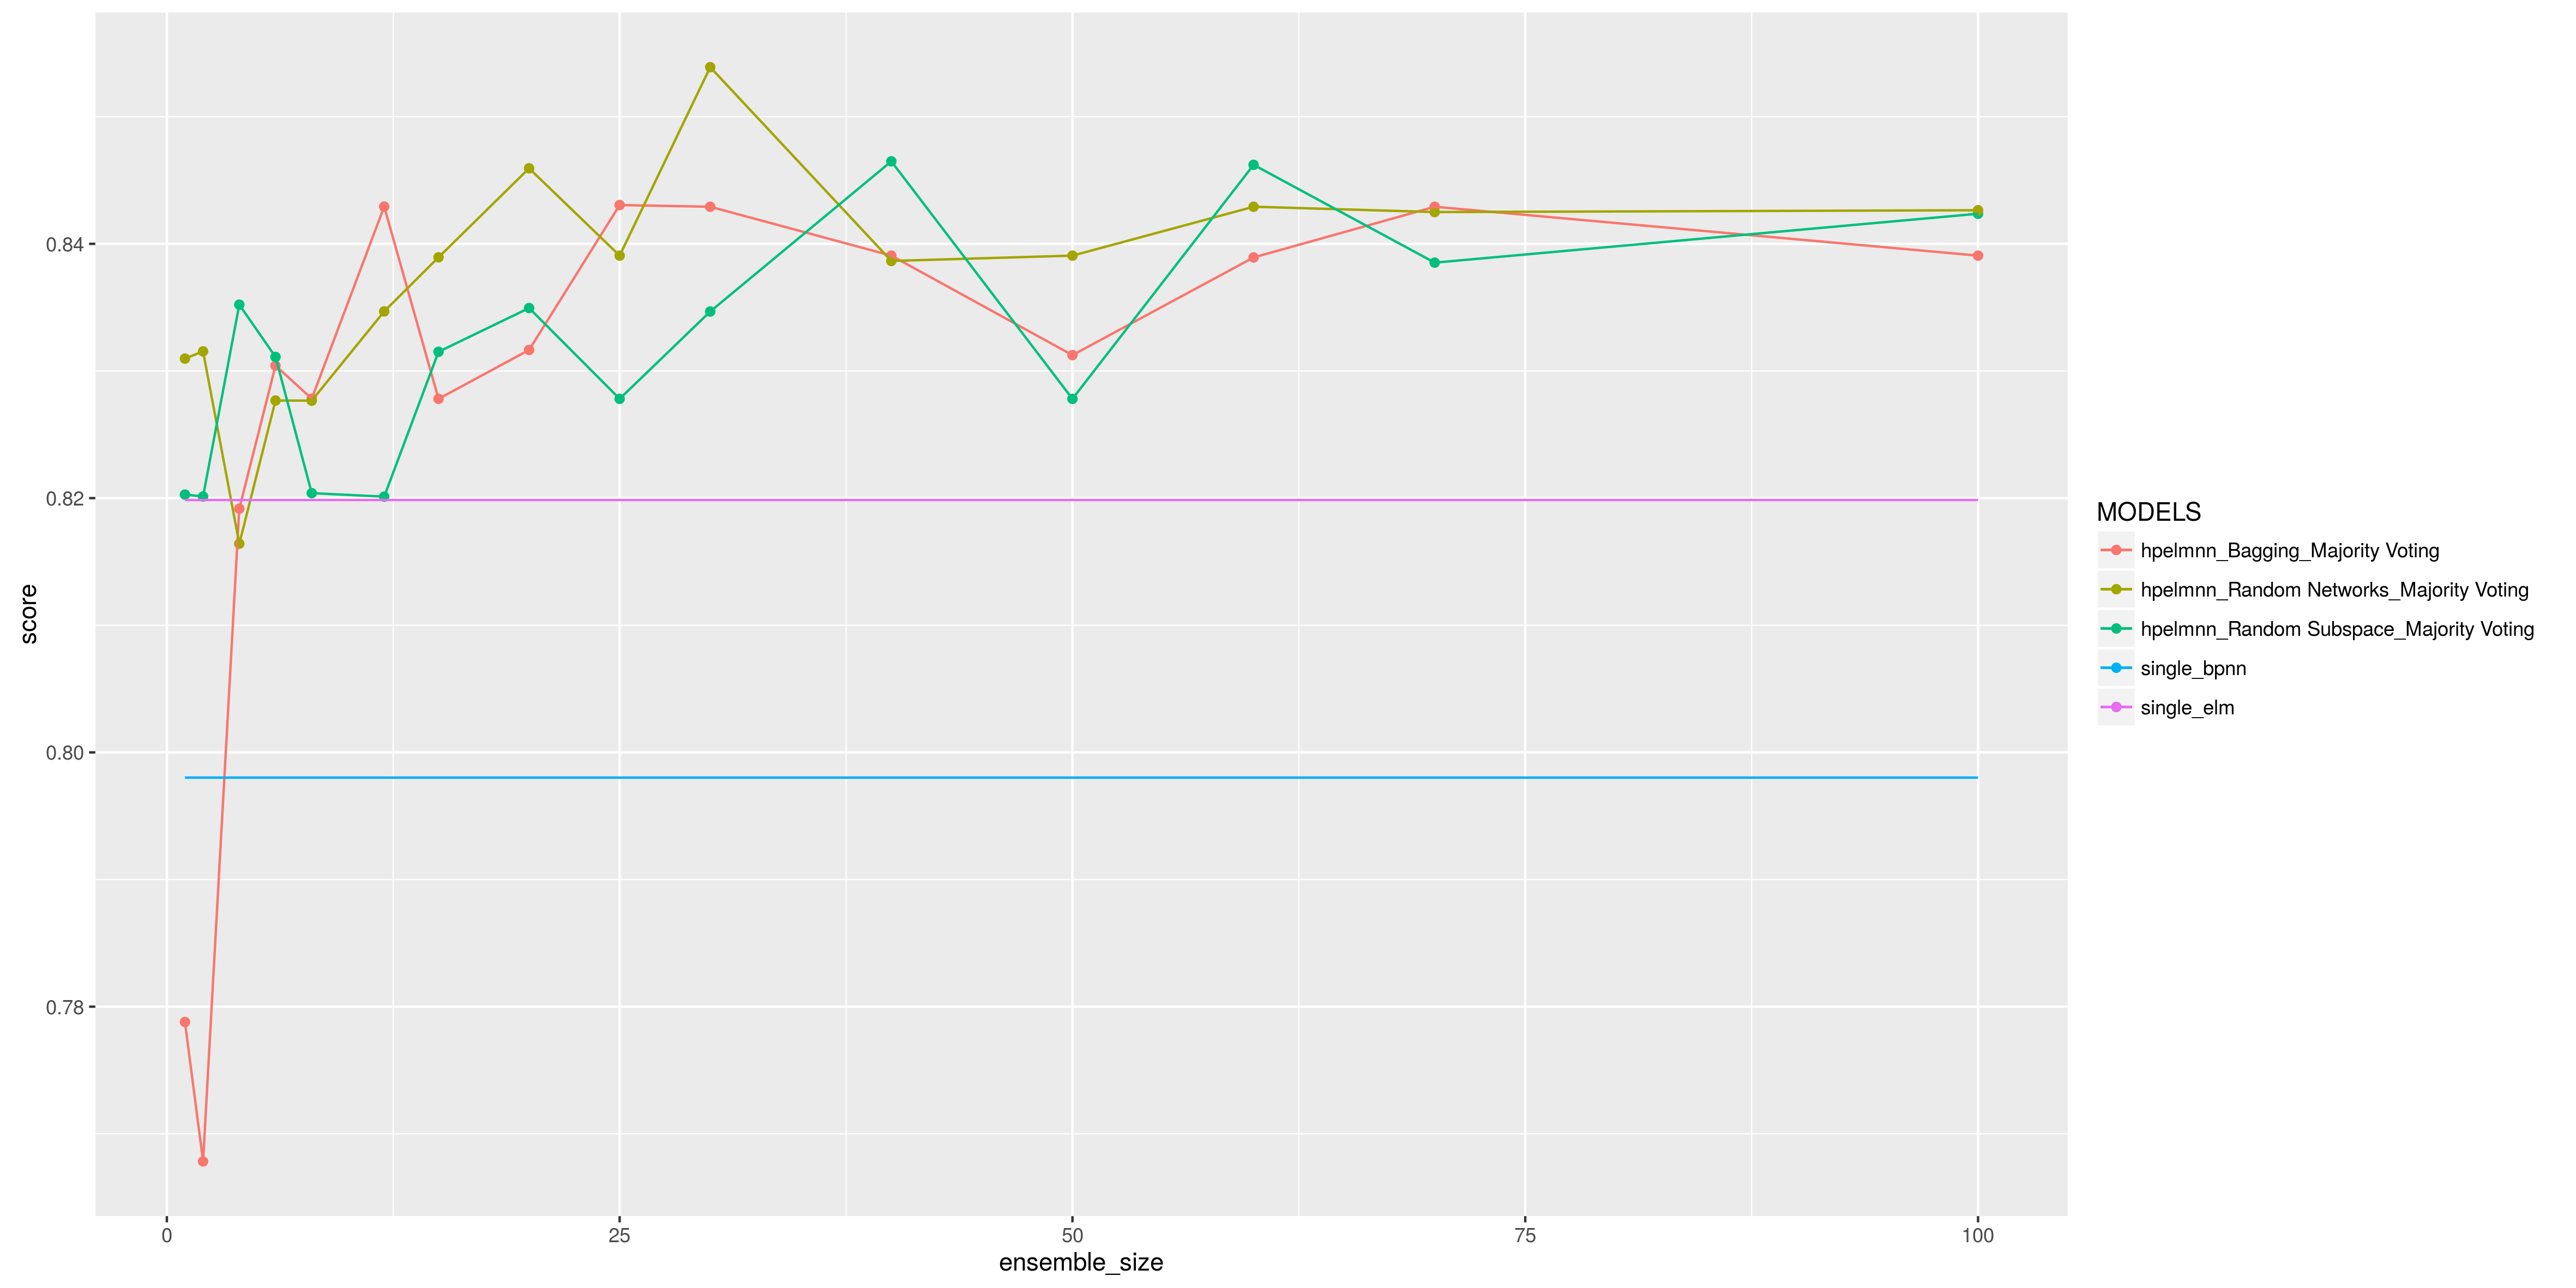
\includegraphics[width=1.0\textwidth]{type4_primary_task_dataset_spect}\centering\caption{spect}\end{figure}
\begin{figure}[H]\includegraphics[width=1.0\textwidth]{type4_primary_task_dataset_thyroid}\centering\caption{thyroid}\end{figure}
\begin{figure}[H]\includegraphics[width=1.0\textwidth]{type4_primary_task_dataset_tic_tac_toe}\centering\caption{tic\_tac\_toe}\end{figure}
\begin{figure}[H]\includegraphics[width=1.0\textwidth]{type4_primary_task_dataset_urban_land_cover}\centering\caption{urban\_land\_cover}\end{figure}
\begin{figure}[H]\includegraphics[width=1.0\textwidth]{type4_primary_task_dataset_wine}\centering\caption{wine}\end{figure}
\begin{figure}[H]\includegraphics[width=1.0\textwidth]{type4_primary_task_dataset_yeast}\centering\caption{yeast}\end{figure}



\begin{thebibliography}{wojcik}
\addcontentsline{toc}{chapter}{Bibliografia}

\bibitem{ELM}
Huang, Guang-Bin and Zhu, Qin-Yu and Siew, Chee Kheong, \textit{Extreme learning machine: Theory and applications.}, Neurocomputing, 2006

\bibitem{ELM_Random}
J. Cao, Z. Lin, G. Bin Huang and N. Liu, \textit{Voting based extreme learning machine}, Inf. Sci. (Ny)., vol. 185, pp. 66-77, 2012
	
\bibitem{HPELM}
Akusok, A. and Bj\"{o}rk, K.-M. and Miche, Y. and Lendasse, A., \textit{High-Performance implementation of an Extreme Learning Machine} [https://pypi.python.org/pypi/hpelm]

\bibitem{scikit-learn}
scikit-learn developers, \textit{Scikit-learn Machine Learning in Python} [http://scikit-learn.org/stable/index.html]

\bibitem{UCI_ML_Repo}
M. Lichman, \textit{UCI Machine Learning Repository} [http://archive.ics.uci.edu/ml], Irvine, CA: University of California, School of Information and Computer Science, 2013
    
\end{thebibliography}

\end{document}